\chapter{Randomized low-rank approximation}
\label{chp:3-nystrom}

Motivate low-rank approximation.

[Plot singular value decay]

%%%%%%%%%%%%%%%%%%%%%%%%%%%%%%%%%%%%%%%%%%%%%%%%%%%%%%%%%%%%%%%%%%%%%%%%%%%%%%%%

\section{The numerical rank of a matrix}
\label{sec:3-nystrom-numerical-rank}

Low-rank structure of matrix.
Formula for $\varepsilon$-numerical rank \cite[Definition~1.1]{noga2013rank} of a matrix $\mtx{B} \in \mathbb{R}^{n \times n}$
\begin{equation}
    r_{\varepsilon, \cdot}(\mtx{B}) = \min \{\rank(\mtx{C}): \mtx{C} \in \mathbb{R}^{n \times n}: \lVert \mtx{B} - \mtx{C} \rVert _{\cdot} \leq \varepsilon \}
    \label{equ:3-nystrom-SS-def-numerical-low-rank}
\end{equation}

For unitarily invariant norms \cite[Theorem~5]{mirsky1960truncation},
Eigenvalues $\mu_1, \dots, \mu_N$ of symmetric matrix $\mtx{B}$
For spectral norm,
\begin{equation}
    r_{\varepsilon, 2}(\mtx{B}) = \min \{1 \leq r \leq N: \mu_{r+1} \leq \varepsilon \}
    \label{equ:3-nystrom-SS-def-numerical-low-rank-spectral-norm}
\end{equation}

For Frobenius norm
\begin{equation}
    r_{\varepsilon, F}(\mtx{B}) = \min \{1 \leq r \leq N: \sqrt{\sum_{j=r+1}^N \mu_{j}^2} \leq \varepsilon \}
    \label{equ:3-nystrom-SS-def-numerical-low-rank-frobenius-norm}
\end{equation}

The eigenvalues of $g_{\sigma}(t\mtx{I} - \mtx{A})$ are
\begin{equation}
    \mu_i(t) = g_{\sigma}(t - \lambda_{(i)}) = \frac{1}{n \sqrt{2 \pi \sigma^2}} e^{-\frac{(t - \lambda_{(i)})^2}{2 \sigma^2}}
\end{equation}
Hence, 
\begin{equation}
    r_{\varepsilon, \cdot}(g_{\sigma}(t\mtx{I} - \mtx{A})) = \#\{1\leq i\leq N: |t - \mu_i(t)| \leq C_{\varepsilon, \cdot}(\sigma)\}
\end{equation}
with the distances
\begin{align}
    C_{\varepsilon, 2}(\sigma) = \sigma \sqrt{-2 \log(N \sqrt{2 \pi} \sigma \varepsilon)} \\
    C_{\varepsilon, F}(\sigma) = \sigma \sqrt{-2 \log(\sqrt{2 \pi} \sigma \varepsilon)}
\end{align}

If we assume the eigenvalues of the matrix $\mtx{A}$ in \refequ{equ:1-introduction-spectral-density-as-trace}
to be evenly distributed in $[a, b]$, i.e. in any subinterval of fixed length in
$[a, b]$ we can expect to find roughly the same number of eigenvalues, then
we can estimate the numerical rank of $g_{\sigma}(t\mtx{I} - \mtx{A})$.
\begin{equation}
    r_{\varepsilon, \cdot}(g_{\sigma}(t\mtx{I} - \mtx{A})) = \frac{2 n}{b - a} C_{\varepsilon, \cdot}(\sigma)
\end{equation}

\begin{figure}[ht]
    \centering
    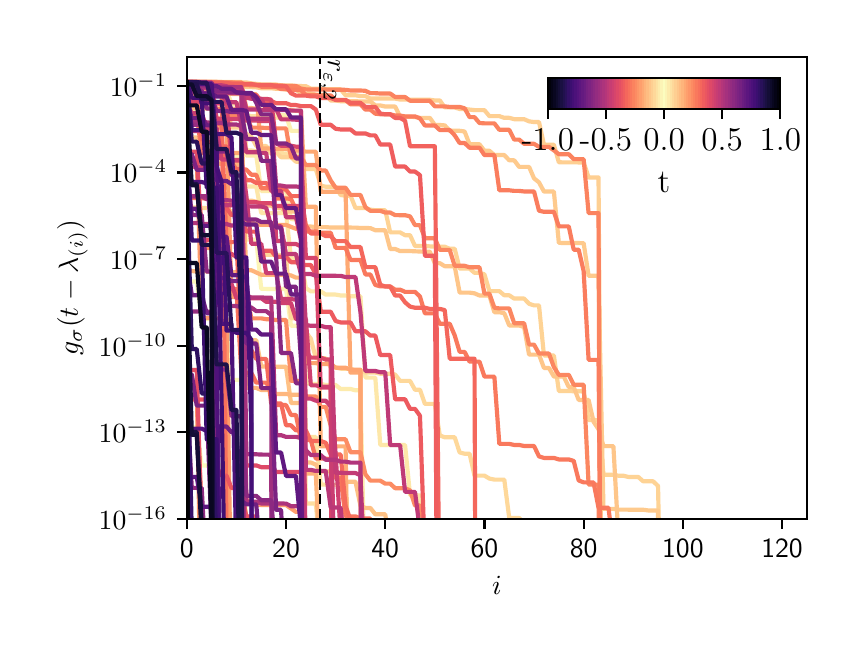
\begin{tikzpicture}
        \node at (0, 0) {%% Creator: Matplotlib, PGF backend
%%
%% To include the figure in your LaTeX document, write
%%   \input{<filename>.pgf}
%%
%% Make sure the required packages are loaded in your preamble
%%   \usepackage{pgf}
%%
%% Also ensure that all the required font packages are loaded; for instance,
%% the lmodern package is sometimes necessary when using math font.
%%   \usepackage{lmodern}
%%
%% Figures using additional raster images can only be included by \input if
%% they are in the same directory as the main LaTeX file. For loading figures
%% from other directories you can use the `import` package
%%   \usepackage{import}
%%
%% and then include the figures with
%%   \import{<path to file>}{<filename>.pgf}
%%
%% Matplotlib used the following preamble
%%   \def\mathdefault#1{#1}
%%   \everymath=\expandafter{\the\everymath\displaystyle}
%%   
%%   \usepackage{fontspec}
%%   \setmainfont{DejaVuSerif.ttf}[Path=\detokenize{C:/Users/fabio/Documents/Work/MasterThesis/Rand-SD/.venv/Lib/site-packages/matplotlib/mpl-data/fonts/ttf/}]
%%   \setsansfont{DejaVuSans.ttf}[Path=\detokenize{C:/Users/fabio/Documents/Work/MasterThesis/Rand-SD/.venv/Lib/site-packages/matplotlib/mpl-data/fonts/ttf/}]
%%   \setmonofont{DejaVuSansMono.ttf}[Path=\detokenize{C:/Users/fabio/Documents/Work/MasterThesis/Rand-SD/.venv/Lib/site-packages/matplotlib/mpl-data/fonts/ttf/}]
%%   \makeatletter\@ifpackageloaded{underscore}{}{\usepackage[strings]{underscore}}\makeatother
%%
\begingroup%
\makeatletter%
\begin{pgfpicture}%
\pgfpathrectangle{\pgfpointorigin}{\pgfqpoint{3.958241in}{2.931603in}}%
\pgfusepath{use as bounding box, clip}%
\begin{pgfscope}%
\pgfsetbuttcap%
\pgfsetmiterjoin%
\definecolor{currentfill}{rgb}{1.000000,1.000000,1.000000}%
\pgfsetfillcolor{currentfill}%
\pgfsetlinewidth{0.000000pt}%
\definecolor{currentstroke}{rgb}{1.000000,1.000000,1.000000}%
\pgfsetstrokecolor{currentstroke}%
\pgfsetdash{}{0pt}%
\pgfpathmoveto{\pgfqpoint{0.000000in}{0.000000in}}%
\pgfpathlineto{\pgfqpoint{3.958241in}{0.000000in}}%
\pgfpathlineto{\pgfqpoint{3.958241in}{2.931603in}}%
\pgfpathlineto{\pgfqpoint{0.000000in}{2.931603in}}%
\pgfpathlineto{\pgfqpoint{0.000000in}{0.000000in}}%
\pgfpathclose%
\pgfusepath{fill}%
\end{pgfscope}%
\begin{pgfscope}%
\pgfsetbuttcap%
\pgfsetmiterjoin%
\definecolor{currentfill}{rgb}{1.000000,1.000000,1.000000}%
\pgfsetfillcolor{currentfill}%
\pgfsetlinewidth{0.000000pt}%
\definecolor{currentstroke}{rgb}{0.000000,0.000000,0.000000}%
\pgfsetstrokecolor{currentstroke}%
\pgfsetstrokeopacity{0.000000}%
\pgfsetdash{}{0pt}%
\pgfpathmoveto{\pgfqpoint{0.749693in}{0.521603in}}%
\pgfpathlineto{\pgfqpoint{3.849693in}{0.521603in}}%
\pgfpathlineto{\pgfqpoint{3.849693in}{2.831603in}}%
\pgfpathlineto{\pgfqpoint{0.749693in}{2.831603in}}%
\pgfpathlineto{\pgfqpoint{0.749693in}{0.521603in}}%
\pgfpathclose%
\pgfusepath{fill}%
\end{pgfscope}%
\begin{pgfscope}%
\pgfsetbuttcap%
\pgfsetroundjoin%
\definecolor{currentfill}{rgb}{0.000000,0.000000,0.000000}%
\pgfsetfillcolor{currentfill}%
\pgfsetlinewidth{0.803000pt}%
\definecolor{currentstroke}{rgb}{0.000000,0.000000,0.000000}%
\pgfsetstrokecolor{currentstroke}%
\pgfsetdash{}{0pt}%
\pgfsys@defobject{currentmarker}{\pgfqpoint{0.000000in}{-0.048611in}}{\pgfqpoint{0.000000in}{0.000000in}}{%
\pgfpathmoveto{\pgfqpoint{0.000000in}{0.000000in}}%
\pgfpathlineto{\pgfqpoint{0.000000in}{-0.048611in}}%
\pgfusepath{stroke,fill}%
}%
\begin{pgfscope}%
\pgfsys@transformshift{0.749693in}{0.521603in}%
\pgfsys@useobject{currentmarker}{}%
\end{pgfscope}%
\end{pgfscope}%
\begin{pgfscope}%
\definecolor{textcolor}{rgb}{0.000000,0.000000,0.000000}%
\pgfsetstrokecolor{textcolor}%
\pgfsetfillcolor{textcolor}%
\pgftext[x=0.749693in,y=0.424381in,,top]{\color{textcolor}{\sffamily\fontsize{10.000000}{12.000000}\selectfont\catcode`\^=\active\def^{\ifmmode\sp\else\^{}\fi}\catcode`\%=\active\def%{\%}0}}%
\end{pgfscope}%
\begin{pgfscope}%
\pgfsetbuttcap%
\pgfsetroundjoin%
\definecolor{currentfill}{rgb}{0.000000,0.000000,0.000000}%
\pgfsetfillcolor{currentfill}%
\pgfsetlinewidth{0.803000pt}%
\definecolor{currentstroke}{rgb}{0.000000,0.000000,0.000000}%
\pgfsetstrokecolor{currentstroke}%
\pgfsetdash{}{0pt}%
\pgfsys@defobject{currentmarker}{\pgfqpoint{0.000000in}{-0.048611in}}{\pgfqpoint{0.000000in}{0.000000in}}{%
\pgfpathmoveto{\pgfqpoint{0.000000in}{0.000000in}}%
\pgfpathlineto{\pgfqpoint{0.000000in}{-0.048611in}}%
\pgfusepath{stroke,fill}%
}%
\begin{pgfscope}%
\pgfsys@transformshift{1.245693in}{0.521603in}%
\pgfsys@useobject{currentmarker}{}%
\end{pgfscope}%
\end{pgfscope}%
\begin{pgfscope}%
\definecolor{textcolor}{rgb}{0.000000,0.000000,0.000000}%
\pgfsetstrokecolor{textcolor}%
\pgfsetfillcolor{textcolor}%
\pgftext[x=1.245693in,y=0.424381in,,top]{\color{textcolor}{\sffamily\fontsize{10.000000}{12.000000}\selectfont\catcode`\^=\active\def^{\ifmmode\sp\else\^{}\fi}\catcode`\%=\active\def%{\%}20}}%
\end{pgfscope}%
\begin{pgfscope}%
\pgfsetbuttcap%
\pgfsetroundjoin%
\definecolor{currentfill}{rgb}{0.000000,0.000000,0.000000}%
\pgfsetfillcolor{currentfill}%
\pgfsetlinewidth{0.803000pt}%
\definecolor{currentstroke}{rgb}{0.000000,0.000000,0.000000}%
\pgfsetstrokecolor{currentstroke}%
\pgfsetdash{}{0pt}%
\pgfsys@defobject{currentmarker}{\pgfqpoint{0.000000in}{-0.048611in}}{\pgfqpoint{0.000000in}{0.000000in}}{%
\pgfpathmoveto{\pgfqpoint{0.000000in}{0.000000in}}%
\pgfpathlineto{\pgfqpoint{0.000000in}{-0.048611in}}%
\pgfusepath{stroke,fill}%
}%
\begin{pgfscope}%
\pgfsys@transformshift{1.741693in}{0.521603in}%
\pgfsys@useobject{currentmarker}{}%
\end{pgfscope}%
\end{pgfscope}%
\begin{pgfscope}%
\definecolor{textcolor}{rgb}{0.000000,0.000000,0.000000}%
\pgfsetstrokecolor{textcolor}%
\pgfsetfillcolor{textcolor}%
\pgftext[x=1.741693in,y=0.424381in,,top]{\color{textcolor}{\sffamily\fontsize{10.000000}{12.000000}\selectfont\catcode`\^=\active\def^{\ifmmode\sp\else\^{}\fi}\catcode`\%=\active\def%{\%}40}}%
\end{pgfscope}%
\begin{pgfscope}%
\pgfsetbuttcap%
\pgfsetroundjoin%
\definecolor{currentfill}{rgb}{0.000000,0.000000,0.000000}%
\pgfsetfillcolor{currentfill}%
\pgfsetlinewidth{0.803000pt}%
\definecolor{currentstroke}{rgb}{0.000000,0.000000,0.000000}%
\pgfsetstrokecolor{currentstroke}%
\pgfsetdash{}{0pt}%
\pgfsys@defobject{currentmarker}{\pgfqpoint{0.000000in}{-0.048611in}}{\pgfqpoint{0.000000in}{0.000000in}}{%
\pgfpathmoveto{\pgfqpoint{0.000000in}{0.000000in}}%
\pgfpathlineto{\pgfqpoint{0.000000in}{-0.048611in}}%
\pgfusepath{stroke,fill}%
}%
\begin{pgfscope}%
\pgfsys@transformshift{2.237693in}{0.521603in}%
\pgfsys@useobject{currentmarker}{}%
\end{pgfscope}%
\end{pgfscope}%
\begin{pgfscope}%
\definecolor{textcolor}{rgb}{0.000000,0.000000,0.000000}%
\pgfsetstrokecolor{textcolor}%
\pgfsetfillcolor{textcolor}%
\pgftext[x=2.237693in,y=0.424381in,,top]{\color{textcolor}{\sffamily\fontsize{10.000000}{12.000000}\selectfont\catcode`\^=\active\def^{\ifmmode\sp\else\^{}\fi}\catcode`\%=\active\def%{\%}60}}%
\end{pgfscope}%
\begin{pgfscope}%
\pgfsetbuttcap%
\pgfsetroundjoin%
\definecolor{currentfill}{rgb}{0.000000,0.000000,0.000000}%
\pgfsetfillcolor{currentfill}%
\pgfsetlinewidth{0.803000pt}%
\definecolor{currentstroke}{rgb}{0.000000,0.000000,0.000000}%
\pgfsetstrokecolor{currentstroke}%
\pgfsetdash{}{0pt}%
\pgfsys@defobject{currentmarker}{\pgfqpoint{0.000000in}{-0.048611in}}{\pgfqpoint{0.000000in}{0.000000in}}{%
\pgfpathmoveto{\pgfqpoint{0.000000in}{0.000000in}}%
\pgfpathlineto{\pgfqpoint{0.000000in}{-0.048611in}}%
\pgfusepath{stroke,fill}%
}%
\begin{pgfscope}%
\pgfsys@transformshift{2.733693in}{0.521603in}%
\pgfsys@useobject{currentmarker}{}%
\end{pgfscope}%
\end{pgfscope}%
\begin{pgfscope}%
\definecolor{textcolor}{rgb}{0.000000,0.000000,0.000000}%
\pgfsetstrokecolor{textcolor}%
\pgfsetfillcolor{textcolor}%
\pgftext[x=2.733693in,y=0.424381in,,top]{\color{textcolor}{\sffamily\fontsize{10.000000}{12.000000}\selectfont\catcode`\^=\active\def^{\ifmmode\sp\else\^{}\fi}\catcode`\%=\active\def%{\%}80}}%
\end{pgfscope}%
\begin{pgfscope}%
\pgfsetbuttcap%
\pgfsetroundjoin%
\definecolor{currentfill}{rgb}{0.000000,0.000000,0.000000}%
\pgfsetfillcolor{currentfill}%
\pgfsetlinewidth{0.803000pt}%
\definecolor{currentstroke}{rgb}{0.000000,0.000000,0.000000}%
\pgfsetstrokecolor{currentstroke}%
\pgfsetdash{}{0pt}%
\pgfsys@defobject{currentmarker}{\pgfqpoint{0.000000in}{-0.048611in}}{\pgfqpoint{0.000000in}{0.000000in}}{%
\pgfpathmoveto{\pgfqpoint{0.000000in}{0.000000in}}%
\pgfpathlineto{\pgfqpoint{0.000000in}{-0.048611in}}%
\pgfusepath{stroke,fill}%
}%
\begin{pgfscope}%
\pgfsys@transformshift{3.229693in}{0.521603in}%
\pgfsys@useobject{currentmarker}{}%
\end{pgfscope}%
\end{pgfscope}%
\begin{pgfscope}%
\definecolor{textcolor}{rgb}{0.000000,0.000000,0.000000}%
\pgfsetstrokecolor{textcolor}%
\pgfsetfillcolor{textcolor}%
\pgftext[x=3.229693in,y=0.424381in,,top]{\color{textcolor}{\sffamily\fontsize{10.000000}{12.000000}\selectfont\catcode`\^=\active\def^{\ifmmode\sp\else\^{}\fi}\catcode`\%=\active\def%{\%}100}}%
\end{pgfscope}%
\begin{pgfscope}%
\pgfsetbuttcap%
\pgfsetroundjoin%
\definecolor{currentfill}{rgb}{0.000000,0.000000,0.000000}%
\pgfsetfillcolor{currentfill}%
\pgfsetlinewidth{0.803000pt}%
\definecolor{currentstroke}{rgb}{0.000000,0.000000,0.000000}%
\pgfsetstrokecolor{currentstroke}%
\pgfsetdash{}{0pt}%
\pgfsys@defobject{currentmarker}{\pgfqpoint{0.000000in}{-0.048611in}}{\pgfqpoint{0.000000in}{0.000000in}}{%
\pgfpathmoveto{\pgfqpoint{0.000000in}{0.000000in}}%
\pgfpathlineto{\pgfqpoint{0.000000in}{-0.048611in}}%
\pgfusepath{stroke,fill}%
}%
\begin{pgfscope}%
\pgfsys@transformshift{3.725693in}{0.521603in}%
\pgfsys@useobject{currentmarker}{}%
\end{pgfscope}%
\end{pgfscope}%
\begin{pgfscope}%
\definecolor{textcolor}{rgb}{0.000000,0.000000,0.000000}%
\pgfsetstrokecolor{textcolor}%
\pgfsetfillcolor{textcolor}%
\pgftext[x=3.725693in,y=0.424381in,,top]{\color{textcolor}{\sffamily\fontsize{10.000000}{12.000000}\selectfont\catcode`\^=\active\def^{\ifmmode\sp\else\^{}\fi}\catcode`\%=\active\def%{\%}120}}%
\end{pgfscope}%
\begin{pgfscope}%
\definecolor{textcolor}{rgb}{0.000000,0.000000,0.000000}%
\pgfsetstrokecolor{textcolor}%
\pgfsetfillcolor{textcolor}%
\pgftext[x=2.299693in,y=0.234413in,,top]{\color{textcolor}{\sffamily\fontsize{10.000000}{12.000000}\selectfont\catcode`\^=\active\def^{\ifmmode\sp\else\^{}\fi}\catcode`\%=\active\def%{\%}$i$}}%
\end{pgfscope}%
\begin{pgfscope}%
\pgfsetbuttcap%
\pgfsetroundjoin%
\definecolor{currentfill}{rgb}{0.000000,0.000000,0.000000}%
\pgfsetfillcolor{currentfill}%
\pgfsetlinewidth{0.803000pt}%
\definecolor{currentstroke}{rgb}{0.000000,0.000000,0.000000}%
\pgfsetstrokecolor{currentstroke}%
\pgfsetdash{}{0pt}%
\pgfsys@defobject{currentmarker}{\pgfqpoint{-0.048611in}{0.000000in}}{\pgfqpoint{-0.000000in}{0.000000in}}{%
\pgfpathmoveto{\pgfqpoint{-0.000000in}{0.000000in}}%
\pgfpathlineto{\pgfqpoint{-0.048611in}{0.000000in}}%
\pgfusepath{stroke,fill}%
}%
\begin{pgfscope}%
\pgfsys@transformshift{0.749693in}{0.521603in}%
\pgfsys@useobject{currentmarker}{}%
\end{pgfscope}%
\end{pgfscope}%
\begin{pgfscope}%
\definecolor{textcolor}{rgb}{0.000000,0.000000,0.000000}%
\pgfsetstrokecolor{textcolor}%
\pgfsetfillcolor{textcolor}%
\pgftext[x=0.309105in, y=0.468842in, left, base]{\color{textcolor}{\sffamily\fontsize{10.000000}{12.000000}\selectfont\catcode`\^=\active\def^{\ifmmode\sp\else\^{}\fi}\catcode`\%=\active\def%{\%}$\mathdefault{10^{-16}}$}}%
\end{pgfscope}%
\begin{pgfscope}%
\pgfsetbuttcap%
\pgfsetroundjoin%
\definecolor{currentfill}{rgb}{0.000000,0.000000,0.000000}%
\pgfsetfillcolor{currentfill}%
\pgfsetlinewidth{0.803000pt}%
\definecolor{currentstroke}{rgb}{0.000000,0.000000,0.000000}%
\pgfsetstrokecolor{currentstroke}%
\pgfsetdash{}{0pt}%
\pgfsys@defobject{currentmarker}{\pgfqpoint{-0.048611in}{0.000000in}}{\pgfqpoint{-0.000000in}{0.000000in}}{%
\pgfpathmoveto{\pgfqpoint{-0.000000in}{0.000000in}}%
\pgfpathlineto{\pgfqpoint{-0.048611in}{0.000000in}}%
\pgfusepath{stroke,fill}%
}%
\begin{pgfscope}%
\pgfsys@transformshift{0.749693in}{0.954728in}%
\pgfsys@useobject{currentmarker}{}%
\end{pgfscope}%
\end{pgfscope}%
\begin{pgfscope}%
\definecolor{textcolor}{rgb}{0.000000,0.000000,0.000000}%
\pgfsetstrokecolor{textcolor}%
\pgfsetfillcolor{textcolor}%
\pgftext[x=0.309105in, y=0.901967in, left, base]{\color{textcolor}{\sffamily\fontsize{10.000000}{12.000000}\selectfont\catcode`\^=\active\def^{\ifmmode\sp\else\^{}\fi}\catcode`\%=\active\def%{\%}$\mathdefault{10^{-13}}$}}%
\end{pgfscope}%
\begin{pgfscope}%
\pgfsetbuttcap%
\pgfsetroundjoin%
\definecolor{currentfill}{rgb}{0.000000,0.000000,0.000000}%
\pgfsetfillcolor{currentfill}%
\pgfsetlinewidth{0.803000pt}%
\definecolor{currentstroke}{rgb}{0.000000,0.000000,0.000000}%
\pgfsetstrokecolor{currentstroke}%
\pgfsetdash{}{0pt}%
\pgfsys@defobject{currentmarker}{\pgfqpoint{-0.048611in}{0.000000in}}{\pgfqpoint{-0.000000in}{0.000000in}}{%
\pgfpathmoveto{\pgfqpoint{-0.000000in}{0.000000in}}%
\pgfpathlineto{\pgfqpoint{-0.048611in}{0.000000in}}%
\pgfusepath{stroke,fill}%
}%
\begin{pgfscope}%
\pgfsys@transformshift{0.749693in}{1.387853in}%
\pgfsys@useobject{currentmarker}{}%
\end{pgfscope}%
\end{pgfscope}%
\begin{pgfscope}%
\definecolor{textcolor}{rgb}{0.000000,0.000000,0.000000}%
\pgfsetstrokecolor{textcolor}%
\pgfsetfillcolor{textcolor}%
\pgftext[x=0.309105in, y=1.335092in, left, base]{\color{textcolor}{\sffamily\fontsize{10.000000}{12.000000}\selectfont\catcode`\^=\active\def^{\ifmmode\sp\else\^{}\fi}\catcode`\%=\active\def%{\%}$\mathdefault{10^{-10}}$}}%
\end{pgfscope}%
\begin{pgfscope}%
\pgfsetbuttcap%
\pgfsetroundjoin%
\definecolor{currentfill}{rgb}{0.000000,0.000000,0.000000}%
\pgfsetfillcolor{currentfill}%
\pgfsetlinewidth{0.803000pt}%
\definecolor{currentstroke}{rgb}{0.000000,0.000000,0.000000}%
\pgfsetstrokecolor{currentstroke}%
\pgfsetdash{}{0pt}%
\pgfsys@defobject{currentmarker}{\pgfqpoint{-0.048611in}{0.000000in}}{\pgfqpoint{-0.000000in}{0.000000in}}{%
\pgfpathmoveto{\pgfqpoint{-0.000000in}{0.000000in}}%
\pgfpathlineto{\pgfqpoint{-0.048611in}{0.000000in}}%
\pgfusepath{stroke,fill}%
}%
\begin{pgfscope}%
\pgfsys@transformshift{0.749693in}{1.820978in}%
\pgfsys@useobject{currentmarker}{}%
\end{pgfscope}%
\end{pgfscope}%
\begin{pgfscope}%
\definecolor{textcolor}{rgb}{0.000000,0.000000,0.000000}%
\pgfsetstrokecolor{textcolor}%
\pgfsetfillcolor{textcolor}%
\pgftext[x=0.364468in, y=1.768217in, left, base]{\color{textcolor}{\sffamily\fontsize{10.000000}{12.000000}\selectfont\catcode`\^=\active\def^{\ifmmode\sp\else\^{}\fi}\catcode`\%=\active\def%{\%}$\mathdefault{10^{-7}}$}}%
\end{pgfscope}%
\begin{pgfscope}%
\pgfsetbuttcap%
\pgfsetroundjoin%
\definecolor{currentfill}{rgb}{0.000000,0.000000,0.000000}%
\pgfsetfillcolor{currentfill}%
\pgfsetlinewidth{0.803000pt}%
\definecolor{currentstroke}{rgb}{0.000000,0.000000,0.000000}%
\pgfsetstrokecolor{currentstroke}%
\pgfsetdash{}{0pt}%
\pgfsys@defobject{currentmarker}{\pgfqpoint{-0.048611in}{0.000000in}}{\pgfqpoint{-0.000000in}{0.000000in}}{%
\pgfpathmoveto{\pgfqpoint{-0.000000in}{0.000000in}}%
\pgfpathlineto{\pgfqpoint{-0.048611in}{0.000000in}}%
\pgfusepath{stroke,fill}%
}%
\begin{pgfscope}%
\pgfsys@transformshift{0.749693in}{2.254103in}%
\pgfsys@useobject{currentmarker}{}%
\end{pgfscope}%
\end{pgfscope}%
\begin{pgfscope}%
\definecolor{textcolor}{rgb}{0.000000,0.000000,0.000000}%
\pgfsetstrokecolor{textcolor}%
\pgfsetfillcolor{textcolor}%
\pgftext[x=0.364468in, y=2.201342in, left, base]{\color{textcolor}{\sffamily\fontsize{10.000000}{12.000000}\selectfont\catcode`\^=\active\def^{\ifmmode\sp\else\^{}\fi}\catcode`\%=\active\def%{\%}$\mathdefault{10^{-4}}$}}%
\end{pgfscope}%
\begin{pgfscope}%
\pgfsetbuttcap%
\pgfsetroundjoin%
\definecolor{currentfill}{rgb}{0.000000,0.000000,0.000000}%
\pgfsetfillcolor{currentfill}%
\pgfsetlinewidth{0.803000pt}%
\definecolor{currentstroke}{rgb}{0.000000,0.000000,0.000000}%
\pgfsetstrokecolor{currentstroke}%
\pgfsetdash{}{0pt}%
\pgfsys@defobject{currentmarker}{\pgfqpoint{-0.048611in}{0.000000in}}{\pgfqpoint{-0.000000in}{0.000000in}}{%
\pgfpathmoveto{\pgfqpoint{-0.000000in}{0.000000in}}%
\pgfpathlineto{\pgfqpoint{-0.048611in}{0.000000in}}%
\pgfusepath{stroke,fill}%
}%
\begin{pgfscope}%
\pgfsys@transformshift{0.749693in}{2.687228in}%
\pgfsys@useobject{currentmarker}{}%
\end{pgfscope}%
\end{pgfscope}%
\begin{pgfscope}%
\definecolor{textcolor}{rgb}{0.000000,0.000000,0.000000}%
\pgfsetstrokecolor{textcolor}%
\pgfsetfillcolor{textcolor}%
\pgftext[x=0.364468in, y=2.634467in, left, base]{\color{textcolor}{\sffamily\fontsize{10.000000}{12.000000}\selectfont\catcode`\^=\active\def^{\ifmmode\sp\else\^{}\fi}\catcode`\%=\active\def%{\%}$\mathdefault{10^{-1}}$}}%
\end{pgfscope}%
\begin{pgfscope}%
\definecolor{textcolor}{rgb}{0.000000,0.000000,0.000000}%
\pgfsetstrokecolor{textcolor}%
\pgfsetfillcolor{textcolor}%
\pgftext[x=0.253550in,y=1.676603in,,bottom,rotate=90.000000]{\color{textcolor}{\sffamily\fontsize{10.000000}{12.000000}\selectfont\catcode`\^=\active\def^{\ifmmode\sp\else\^{}\fi}\catcode`\%=\active\def%{\%}$g_{\sigma}(t - \lambda_{(i)})$}}%
\end{pgfscope}%
\begin{pgfscope}%
\pgfpathrectangle{\pgfqpoint{0.749693in}{0.521603in}}{\pgfqpoint{3.100000in}{2.310000in}}%
\pgfusepath{clip}%
\pgfsetrectcap%
\pgfsetroundjoin%
\pgfsetlinewidth{1.505625pt}%
\definecolor{currentstroke}{rgb}{0.987053,0.991438,0.749504}%
\pgfsetstrokecolor{currentstroke}%
\pgfsetdash{}{0pt}%
\pgfpathmoveto{\pgfqpoint{0.749693in}{0.980593in}}%
\pgfpathlineto{\pgfqpoint{0.799293in}{0.980290in}}%
\pgfpathlineto{\pgfqpoint{0.824093in}{0.788421in}}%
\pgfpathlineto{\pgfqpoint{0.948093in}{0.788386in}}%
\pgfpathlineto{\pgfqpoint{0.968223in}{0.511603in}}%
\pgfpathlineto{\pgfqpoint{0.968223in}{0.511603in}}%
\pgfusepath{stroke}%
\end{pgfscope}%
\begin{pgfscope}%
\pgfpathrectangle{\pgfqpoint{0.749693in}{0.521603in}}{\pgfqpoint{3.100000in}{2.310000in}}%
\pgfusepath{clip}%
\pgfsetrectcap%
\pgfsetroundjoin%
\pgfsetlinewidth{1.505625pt}%
\definecolor{currentstroke}{rgb}{0.987691,0.977154,0.734536}%
\pgfsetstrokecolor{currentstroke}%
\pgfsetdash{}{0pt}%
\pgfpathmoveto{\pgfqpoint{0.749693in}{1.709115in}}%
\pgfpathlineto{\pgfqpoint{0.799293in}{1.708387in}}%
\pgfpathlineto{\pgfqpoint{0.824093in}{1.520385in}}%
\pgfpathlineto{\pgfqpoint{0.948093in}{1.520345in}}%
\pgfpathlineto{\pgfqpoint{0.972893in}{1.217082in}}%
\pgfpathlineto{\pgfqpoint{1.022493in}{1.216187in}}%
\pgfpathlineto{\pgfqpoint{1.045763in}{0.511603in}}%
\pgfpathlineto{\pgfqpoint{1.045763in}{0.511603in}}%
\pgfusepath{stroke}%
\end{pgfscope}%
\begin{pgfscope}%
\pgfpathrectangle{\pgfqpoint{0.749693in}{0.521603in}}{\pgfqpoint{3.100000in}{2.310000in}}%
\pgfusepath{clip}%
\pgfsetrectcap%
\pgfsetroundjoin%
\pgfsetlinewidth{1.505625pt}%
\definecolor{currentstroke}{rgb}{0.988717,0.955742,0.712242}%
\pgfsetstrokecolor{currentstroke}%
\pgfsetdash{}{0pt}%
\pgfpathmoveto{\pgfqpoint{0.749693in}{2.554702in}}%
\pgfpathlineto{\pgfqpoint{0.799293in}{2.554418in}}%
\pgfpathlineto{\pgfqpoint{0.824093in}{2.476100in}}%
\pgfpathlineto{\pgfqpoint{0.948093in}{2.476083in}}%
\pgfpathlineto{\pgfqpoint{0.972893in}{2.332790in}}%
\pgfpathlineto{\pgfqpoint{1.022493in}{2.332341in}}%
\pgfpathlineto{\pgfqpoint{1.047293in}{1.918026in}}%
\pgfpathlineto{\pgfqpoint{1.096893in}{1.918026in}}%
\pgfpathlineto{\pgfqpoint{1.121693in}{1.671646in}}%
\pgfpathlineto{\pgfqpoint{1.245693in}{1.670905in}}%
\pgfpathlineto{\pgfqpoint{1.270493in}{1.487623in}}%
\pgfpathlineto{\pgfqpoint{1.320093in}{1.487623in}}%
\pgfpathlineto{\pgfqpoint{1.325178in}{0.511603in}}%
\pgfpathlineto{\pgfqpoint{1.325178in}{0.511603in}}%
\pgfusepath{stroke}%
\end{pgfscope}%
\begin{pgfscope}%
\pgfpathrectangle{\pgfqpoint{0.749693in}{0.521603in}}{\pgfqpoint{3.100000in}{2.310000in}}%
\pgfusepath{clip}%
\pgfsetrectcap%
\pgfsetroundjoin%
\pgfsetlinewidth{1.505625pt}%
\definecolor{currentstroke}{rgb}{0.989434,0.941470,0.697519}%
\pgfsetstrokecolor{currentstroke}%
\pgfsetdash{}{0pt}%
\pgfpathmoveto{\pgfqpoint{0.749693in}{2.706444in}}%
\pgfpathlineto{\pgfqpoint{0.799293in}{2.706442in}}%
\pgfpathlineto{\pgfqpoint{0.824093in}{2.689767in}}%
\pgfpathlineto{\pgfqpoint{0.948093in}{2.689762in}}%
\pgfpathlineto{\pgfqpoint{0.972893in}{2.658396in}}%
\pgfpathlineto{\pgfqpoint{1.022493in}{2.658236in}}%
\pgfpathlineto{\pgfqpoint{1.047293in}{2.628712in}}%
\pgfpathlineto{\pgfqpoint{1.096893in}{2.628712in}}%
\pgfpathlineto{\pgfqpoint{1.121693in}{2.539876in}}%
\pgfpathlineto{\pgfqpoint{1.245693in}{2.539578in}}%
\pgfpathlineto{\pgfqpoint{1.270493in}{2.461537in}}%
\pgfpathlineto{\pgfqpoint{1.320093in}{2.461537in}}%
\pgfpathlineto{\pgfqpoint{1.335563in}{0.511603in}}%
\pgfpathlineto{\pgfqpoint{1.335563in}{0.511603in}}%
\pgfusepath{stroke}%
\end{pgfscope}%
\begin{pgfscope}%
\pgfpathrectangle{\pgfqpoint{0.749693in}{0.521603in}}{\pgfqpoint{3.100000in}{2.310000in}}%
\pgfusepath{clip}%
\pgfsetrectcap%
\pgfsetroundjoin%
\pgfsetlinewidth{1.505625pt}%
\definecolor{currentstroke}{rgb}{0.990570,0.920049,0.675675}%
\pgfsetstrokecolor{currentstroke}%
\pgfsetdash{}{0pt}%
\pgfpathmoveto{\pgfqpoint{0.749693in}{2.693399in}}%
\pgfpathlineto{\pgfqpoint{0.799293in}{2.693399in}}%
\pgfpathlineto{\pgfqpoint{0.824093in}{2.666199in}}%
\pgfpathlineto{\pgfqpoint{0.948093in}{2.666052in}}%
\pgfpathlineto{\pgfqpoint{0.972893in}{2.597345in}}%
\pgfpathlineto{\pgfqpoint{1.022493in}{2.597345in}}%
\pgfpathlineto{\pgfqpoint{1.047293in}{2.338490in}}%
\pgfpathlineto{\pgfqpoint{1.096893in}{2.338045in}}%
\pgfpathlineto{\pgfqpoint{1.121693in}{2.161398in}}%
\pgfpathlineto{\pgfqpoint{1.245693in}{2.161371in}}%
\pgfpathlineto{\pgfqpoint{1.270493in}{2.020320in}}%
\pgfpathlineto{\pgfqpoint{1.320093in}{2.019716in}}%
\pgfpathlineto{\pgfqpoint{1.344893in}{1.201349in}}%
\pgfpathlineto{\pgfqpoint{1.369693in}{1.196889in}}%
\pgfpathlineto{\pgfqpoint{1.419293in}{1.196889in}}%
\pgfpathlineto{\pgfqpoint{1.444093in}{1.191212in}}%
\pgfpathlineto{\pgfqpoint{1.493693in}{1.191212in}}%
\pgfpathlineto{\pgfqpoint{1.518493in}{1.171097in}}%
\pgfpathlineto{\pgfqpoint{1.568093in}{1.171097in}}%
\pgfpathlineto{\pgfqpoint{1.592893in}{1.164460in}}%
\pgfpathlineto{\pgfqpoint{1.617693in}{1.164460in}}%
\pgfpathlineto{\pgfqpoint{1.632460in}{0.511603in}}%
\pgfpathlineto{\pgfqpoint{1.632460in}{0.511603in}}%
\pgfusepath{stroke}%
\end{pgfscope}%
\begin{pgfscope}%
\pgfpathrectangle{\pgfqpoint{0.749693in}{0.521603in}}{\pgfqpoint{3.100000in}{2.310000in}}%
\pgfusepath{clip}%
\pgfsetrectcap%
\pgfsetroundjoin%
\pgfsetlinewidth{1.505625pt}%
\definecolor{currentstroke}{rgb}{0.991332,0.905763,0.661309}%
\pgfsetstrokecolor{currentstroke}%
\pgfsetdash{}{0pt}%
\pgfpathmoveto{\pgfqpoint{0.749693in}{2.324888in}}%
\pgfpathlineto{\pgfqpoint{0.774493in}{2.322641in}}%
\pgfpathlineto{\pgfqpoint{0.824093in}{2.322641in}}%
\pgfpathlineto{\pgfqpoint{0.848893in}{2.319776in}}%
\pgfpathlineto{\pgfqpoint{0.898493in}{2.319776in}}%
\pgfpathlineto{\pgfqpoint{0.923293in}{2.309582in}}%
\pgfpathlineto{\pgfqpoint{0.972893in}{2.309582in}}%
\pgfpathlineto{\pgfqpoint{0.997693in}{2.306204in}}%
\pgfpathlineto{\pgfqpoint{1.022493in}{2.306204in}}%
\pgfpathlineto{\pgfqpoint{1.047293in}{2.183207in}}%
\pgfpathlineto{\pgfqpoint{1.096893in}{2.183207in}}%
\pgfpathlineto{\pgfqpoint{1.121693in}{2.050766in}}%
\pgfpathlineto{\pgfqpoint{1.245693in}{2.050176in}}%
\pgfpathlineto{\pgfqpoint{1.270493in}{1.823925in}}%
\pgfpathlineto{\pgfqpoint{1.320093in}{1.823925in}}%
\pgfpathlineto{\pgfqpoint{1.344893in}{1.675860in}}%
\pgfpathlineto{\pgfqpoint{1.369693in}{1.659130in}}%
\pgfpathlineto{\pgfqpoint{1.419293in}{1.659130in}}%
\pgfpathlineto{\pgfqpoint{1.444093in}{1.643181in}}%
\pgfpathlineto{\pgfqpoint{1.493693in}{1.643181in}}%
\pgfpathlineto{\pgfqpoint{1.518493in}{1.638771in}}%
\pgfpathlineto{\pgfqpoint{1.543293in}{1.638771in}}%
\pgfpathlineto{\pgfqpoint{1.568093in}{1.635204in}}%
\pgfpathlineto{\pgfqpoint{1.617693in}{1.635204in}}%
\pgfpathlineto{\pgfqpoint{1.642493in}{1.228484in}}%
\pgfpathlineto{\pgfqpoint{1.692093in}{1.227592in}}%
\pgfpathlineto{\pgfqpoint{1.716893in}{0.890977in}}%
\pgfpathlineto{\pgfqpoint{1.840893in}{0.890927in}}%
\pgfpathlineto{\pgfqpoint{1.865693in}{0.640192in}}%
\pgfpathlineto{\pgfqpoint{1.915293in}{0.639144in}}%
\pgfpathlineto{\pgfqpoint{1.915917in}{0.511603in}}%
\pgfpathlineto{\pgfqpoint{1.915917in}{0.511603in}}%
\pgfusepath{stroke}%
\end{pgfscope}%
\begin{pgfscope}%
\pgfpathrectangle{\pgfqpoint{0.749693in}{0.521603in}}{\pgfqpoint{3.100000in}{2.310000in}}%
\pgfusepath{clip}%
\pgfsetrectcap%
\pgfsetroundjoin%
\pgfsetlinewidth{1.505625pt}%
\definecolor{currentstroke}{rgb}{0.992440,0.884330,0.640099}%
\pgfsetstrokecolor{currentstroke}%
\pgfsetdash{}{0pt}%
\pgfpathmoveto{\pgfqpoint{0.749693in}{2.706374in}}%
\pgfpathlineto{\pgfqpoint{1.022493in}{2.705895in}}%
\pgfpathlineto{\pgfqpoint{1.047293in}{2.541564in}}%
\pgfpathlineto{\pgfqpoint{1.072093in}{2.534832in}}%
\pgfpathlineto{\pgfqpoint{1.121693in}{2.534832in}}%
\pgfpathlineto{\pgfqpoint{1.146493in}{2.528340in}}%
\pgfpathlineto{\pgfqpoint{1.196093in}{2.528340in}}%
\pgfpathlineto{\pgfqpoint{1.220893in}{2.526532in}}%
\pgfpathlineto{\pgfqpoint{1.245693in}{2.526532in}}%
\pgfpathlineto{\pgfqpoint{1.270493in}{2.525066in}}%
\pgfpathlineto{\pgfqpoint{1.320093in}{2.525066in}}%
\pgfpathlineto{\pgfqpoint{1.344893in}{0.930962in}}%
\pgfpathlineto{\pgfqpoint{1.394493in}{0.930962in}}%
\pgfpathlineto{\pgfqpoint{1.419293in}{0.693281in}}%
\pgfpathlineto{\pgfqpoint{1.543293in}{0.692246in}}%
\pgfpathlineto{\pgfqpoint{1.554965in}{0.511603in}}%
\pgfpathlineto{\pgfqpoint{1.554965in}{0.511603in}}%
\pgfusepath{stroke}%
\end{pgfscope}%
\begin{pgfscope}%
\pgfpathrectangle{\pgfqpoint{0.749693in}{0.521603in}}{\pgfqpoint{3.100000in}{2.310000in}}%
\pgfusepath{clip}%
\pgfsetrectcap%
\pgfsetroundjoin%
\pgfsetlinewidth{1.505625pt}%
\definecolor{currentstroke}{rgb}{0.993170,0.870024,0.626189}%
\pgfsetstrokecolor{currentstroke}%
\pgfsetdash{}{0pt}%
\pgfpathmoveto{\pgfqpoint{0.749693in}{2.672875in}}%
\pgfpathlineto{\pgfqpoint{0.848893in}{2.672240in}}%
\pgfpathlineto{\pgfqpoint{0.898493in}{2.671445in}}%
\pgfpathlineto{\pgfqpoint{0.923293in}{2.671445in}}%
\pgfpathlineto{\pgfqpoint{0.948093in}{2.668480in}}%
\pgfpathlineto{\pgfqpoint{0.997693in}{2.668480in}}%
\pgfpathlineto{\pgfqpoint{1.022493in}{2.665215in}}%
\pgfpathlineto{\pgfqpoint{1.047293in}{2.363532in}}%
\pgfpathlineto{\pgfqpoint{1.072093in}{2.363532in}}%
\pgfpathlineto{\pgfqpoint{1.096893in}{2.360392in}}%
\pgfpathlineto{\pgfqpoint{1.146493in}{2.360392in}}%
\pgfpathlineto{\pgfqpoint{1.171293in}{2.350744in}}%
\pgfpathlineto{\pgfqpoint{1.220893in}{2.350744in}}%
\pgfpathlineto{\pgfqpoint{1.245693in}{2.347986in}}%
\pgfpathlineto{\pgfqpoint{1.295293in}{2.347986in}}%
\pgfpathlineto{\pgfqpoint{1.320093in}{2.345807in}}%
\pgfpathlineto{\pgfqpoint{1.344893in}{0.598521in}}%
\pgfpathlineto{\pgfqpoint{1.394493in}{0.598521in}}%
\pgfpathlineto{\pgfqpoint{1.402792in}{0.511603in}}%
\pgfpathlineto{\pgfqpoint{1.402792in}{0.511603in}}%
\pgfusepath{stroke}%
\end{pgfscope}%
\begin{pgfscope}%
\pgfpathrectangle{\pgfqpoint{0.749693in}{0.521603in}}{\pgfqpoint{3.100000in}{2.310000in}}%
\pgfusepath{clip}%
\pgfsetrectcap%
\pgfsetroundjoin%
\pgfsetlinewidth{1.505625pt}%
\definecolor{currentstroke}{rgb}{0.994222,0.848540,0.605696}%
\pgfsetstrokecolor{currentstroke}%
\pgfsetdash{}{0pt}%
\pgfpathmoveto{\pgfqpoint{0.749693in}{2.078631in}}%
\pgfpathlineto{\pgfqpoint{0.799293in}{2.078631in}}%
\pgfpathlineto{\pgfqpoint{0.824093in}{2.075895in}}%
\pgfpathlineto{\pgfqpoint{0.848893in}{2.075895in}}%
\pgfpathlineto{\pgfqpoint{0.873693in}{2.072498in}}%
\pgfpathlineto{\pgfqpoint{0.923293in}{2.072498in}}%
\pgfpathlineto{\pgfqpoint{0.948093in}{2.060076in}}%
\pgfpathlineto{\pgfqpoint{0.997693in}{2.060076in}}%
\pgfpathlineto{\pgfqpoint{1.022493in}{2.046813in}}%
\pgfpathlineto{\pgfqpoint{1.047293in}{1.996220in}}%
\pgfpathlineto{\pgfqpoint{1.096893in}{1.996220in}}%
\pgfpathlineto{\pgfqpoint{1.121693in}{1.842290in}}%
\pgfpathlineto{\pgfqpoint{1.171293in}{1.842290in}}%
\pgfpathlineto{\pgfqpoint{1.196093in}{1.841153in}}%
\pgfpathlineto{\pgfqpoint{1.245693in}{1.841153in}}%
\pgfpathlineto{\pgfqpoint{1.270493in}{1.524894in}}%
\pgfpathlineto{\pgfqpoint{1.320093in}{1.524894in}}%
\pgfpathlineto{\pgfqpoint{1.344893in}{1.455081in}}%
\pgfpathlineto{\pgfqpoint{1.369693in}{1.422826in}}%
\pgfpathlineto{\pgfqpoint{1.394493in}{1.324634in}}%
\pgfpathlineto{\pgfqpoint{1.444093in}{1.324634in}}%
\pgfpathlineto{\pgfqpoint{1.468893in}{1.279117in}}%
\pgfpathlineto{\pgfqpoint{1.493693in}{1.279117in}}%
\pgfpathlineto{\pgfqpoint{1.518493in}{1.272717in}}%
\pgfpathlineto{\pgfqpoint{1.568093in}{1.272717in}}%
\pgfpathlineto{\pgfqpoint{1.592893in}{1.263404in}}%
\pgfpathlineto{\pgfqpoint{1.617693in}{1.263404in}}%
\pgfpathlineto{\pgfqpoint{1.642493in}{1.253149in}}%
\pgfpathlineto{\pgfqpoint{1.692093in}{1.253149in}}%
\pgfpathlineto{\pgfqpoint{1.716893in}{1.247579in}}%
\pgfpathlineto{\pgfqpoint{1.766493in}{1.247579in}}%
\pgfpathlineto{\pgfqpoint{1.791293in}{1.243187in}}%
\pgfpathlineto{\pgfqpoint{1.816093in}{1.211530in}}%
\pgfpathlineto{\pgfqpoint{1.865693in}{1.211530in}}%
\pgfpathlineto{\pgfqpoint{1.890493in}{1.167261in}}%
\pgfpathlineto{\pgfqpoint{1.915293in}{1.167261in}}%
\pgfpathlineto{\pgfqpoint{1.940093in}{1.096592in}}%
\pgfpathlineto{\pgfqpoint{1.989693in}{1.096592in}}%
\pgfpathlineto{\pgfqpoint{2.014493in}{0.938712in}}%
\pgfpathlineto{\pgfqpoint{2.039293in}{0.929730in}}%
\pgfpathlineto{\pgfqpoint{2.088893in}{0.929730in}}%
\pgfpathlineto{\pgfqpoint{2.113693in}{0.853871in}}%
\pgfpathlineto{\pgfqpoint{2.138493in}{0.847608in}}%
\pgfpathlineto{\pgfqpoint{2.163293in}{0.847608in}}%
\pgfpathlineto{\pgfqpoint{2.188093in}{0.737866in}}%
\pgfpathlineto{\pgfqpoint{2.237693in}{0.737866in}}%
\pgfpathlineto{\pgfqpoint{2.262493in}{0.723060in}}%
\pgfpathlineto{\pgfqpoint{2.287293in}{0.718168in}}%
\pgfpathlineto{\pgfqpoint{2.336893in}{0.718168in}}%
\pgfpathlineto{\pgfqpoint{2.361693in}{0.526213in}}%
\pgfpathlineto{\pgfqpoint{2.411293in}{0.526213in}}%
\pgfpathlineto{\pgfqpoint{2.426649in}{0.511603in}}%
\pgfpathlineto{\pgfqpoint{2.426649in}{0.511603in}}%
\pgfusepath{stroke}%
\end{pgfscope}%
\begin{pgfscope}%
\pgfpathrectangle{\pgfqpoint{0.749693in}{0.521603in}}{\pgfqpoint{3.100000in}{2.310000in}}%
\pgfusepath{clip}%
\pgfsetrectcap%
\pgfsetroundjoin%
\pgfsetlinewidth{1.505625pt}%
\definecolor{currentstroke}{rgb}{0.995131,0.827052,0.585701}%
\pgfsetstrokecolor{currentstroke}%
\pgfsetdash{}{0pt}%
\pgfpathmoveto{\pgfqpoint{0.749693in}{2.651865in}}%
\pgfpathlineto{\pgfqpoint{0.799293in}{2.651865in}}%
\pgfpathlineto{\pgfqpoint{0.824093in}{2.603740in}}%
\pgfpathlineto{\pgfqpoint{0.948093in}{2.603347in}}%
\pgfpathlineto{\pgfqpoint{0.972893in}{2.478085in}}%
\pgfpathlineto{\pgfqpoint{1.022493in}{2.478085in}}%
\pgfpathlineto{\pgfqpoint{1.047293in}{2.446832in}}%
\pgfpathlineto{\pgfqpoint{1.072093in}{2.432028in}}%
\pgfpathlineto{\pgfqpoint{1.096893in}{2.385655in}}%
\pgfpathlineto{\pgfqpoint{1.146493in}{2.385655in}}%
\pgfpathlineto{\pgfqpoint{1.171293in}{2.355809in}}%
\pgfpathlineto{\pgfqpoint{1.196093in}{2.355809in}}%
\pgfpathlineto{\pgfqpoint{1.220893in}{2.330006in}}%
\pgfpathlineto{\pgfqpoint{1.270493in}{2.330006in}}%
\pgfpathlineto{\pgfqpoint{1.295293in}{2.307630in}}%
\pgfpathlineto{\pgfqpoint{1.320093in}{2.307630in}}%
\pgfpathlineto{\pgfqpoint{1.344893in}{2.271269in}}%
\pgfpathlineto{\pgfqpoint{1.394493in}{2.271269in}}%
\pgfpathlineto{\pgfqpoint{1.419293in}{2.187410in}}%
\pgfpathlineto{\pgfqpoint{1.444093in}{2.182538in}}%
\pgfpathlineto{\pgfqpoint{1.493693in}{2.182538in}}%
\pgfpathlineto{\pgfqpoint{1.518493in}{2.140982in}}%
\pgfpathlineto{\pgfqpoint{1.543293in}{2.137520in}}%
\pgfpathlineto{\pgfqpoint{1.568093in}{2.137520in}}%
\pgfpathlineto{\pgfqpoint{1.592893in}{2.076104in}}%
\pgfpathlineto{\pgfqpoint{1.642493in}{2.076104in}}%
\pgfpathlineto{\pgfqpoint{1.667293in}{2.067714in}}%
\pgfpathlineto{\pgfqpoint{1.692093in}{2.064936in}}%
\pgfpathlineto{\pgfqpoint{1.741693in}{2.064936in}}%
\pgfpathlineto{\pgfqpoint{1.766493in}{1.953992in}}%
\pgfpathlineto{\pgfqpoint{1.816093in}{1.953992in}}%
\pgfpathlineto{\pgfqpoint{1.840893in}{1.940104in}}%
\pgfpathlineto{\pgfqpoint{1.865693in}{1.940104in}}%
\pgfpathlineto{\pgfqpoint{1.890493in}{1.885857in}}%
\pgfpathlineto{\pgfqpoint{1.940093in}{1.885857in}}%
\pgfpathlineto{\pgfqpoint{1.989693in}{1.882489in}}%
\pgfpathlineto{\pgfqpoint{2.039293in}{1.882489in}}%
\pgfpathlineto{\pgfqpoint{2.064093in}{1.872065in}}%
\pgfpathlineto{\pgfqpoint{2.088893in}{1.872065in}}%
\pgfpathlineto{\pgfqpoint{2.113693in}{1.773056in}}%
\pgfpathlineto{\pgfqpoint{2.163293in}{1.773056in}}%
\pgfpathlineto{\pgfqpoint{2.188093in}{1.751946in}}%
\pgfpathlineto{\pgfqpoint{2.212893in}{1.751946in}}%
\pgfpathlineto{\pgfqpoint{2.237693in}{1.744421in}}%
\pgfpathlineto{\pgfqpoint{2.262493in}{1.660597in}}%
\pgfpathlineto{\pgfqpoint{2.312093in}{1.660597in}}%
\pgfpathlineto{\pgfqpoint{2.336893in}{1.639657in}}%
\pgfpathlineto{\pgfqpoint{2.361693in}{1.639657in}}%
\pgfpathlineto{\pgfqpoint{2.386493in}{1.623234in}}%
\pgfpathlineto{\pgfqpoint{2.436093in}{1.623234in}}%
\pgfpathlineto{\pgfqpoint{2.460893in}{1.597133in}}%
\pgfpathlineto{\pgfqpoint{2.485693in}{1.589179in}}%
\pgfpathlineto{\pgfqpoint{2.510493in}{1.589179in}}%
\pgfpathlineto{\pgfqpoint{2.535293in}{1.338681in}}%
\pgfpathlineto{\pgfqpoint{2.584893in}{1.338681in}}%
\pgfpathlineto{\pgfqpoint{2.609693in}{1.161060in}}%
\pgfpathlineto{\pgfqpoint{2.659293in}{1.161060in}}%
\pgfpathlineto{\pgfqpoint{2.684093in}{1.159810in}}%
\pgfpathlineto{\pgfqpoint{2.733693in}{1.159810in}}%
\pgfpathlineto{\pgfqpoint{2.758493in}{1.016030in}}%
\pgfpathlineto{\pgfqpoint{2.808093in}{1.016030in}}%
\pgfpathlineto{\pgfqpoint{2.832893in}{0.742334in}}%
\pgfpathlineto{\pgfqpoint{2.882493in}{0.742334in}}%
\pgfpathlineto{\pgfqpoint{2.907293in}{0.737497in}}%
\pgfpathlineto{\pgfqpoint{2.932093in}{0.737497in}}%
\pgfpathlineto{\pgfqpoint{2.956893in}{0.731498in}}%
\pgfpathlineto{\pgfqpoint{3.006493in}{0.731498in}}%
\pgfpathlineto{\pgfqpoint{3.031293in}{0.709618in}}%
\pgfpathlineto{\pgfqpoint{3.080893in}{0.709618in}}%
\pgfpathlineto{\pgfqpoint{3.105693in}{0.686358in}}%
\pgfpathlineto{\pgfqpoint{3.109206in}{0.511603in}}%
\pgfpathlineto{\pgfqpoint{3.109206in}{0.511603in}}%
\pgfusepath{stroke}%
\end{pgfscope}%
\begin{pgfscope}%
\pgfpathrectangle{\pgfqpoint{0.749693in}{0.521603in}}{\pgfqpoint{3.100000in}{2.310000in}}%
\pgfusepath{clip}%
\pgfsetrectcap%
\pgfsetroundjoin%
\pgfsetlinewidth{1.505625pt}%
\definecolor{currentstroke}{rgb}{0.995680,0.812706,0.572645}%
\pgfsetstrokecolor{currentstroke}%
\pgfsetdash{}{0pt}%
\pgfpathmoveto{\pgfqpoint{0.749693in}{2.706429in}}%
\pgfpathlineto{\pgfqpoint{0.898493in}{2.705946in}}%
\pgfpathlineto{\pgfqpoint{0.923293in}{2.704622in}}%
\pgfpathlineto{\pgfqpoint{1.047293in}{2.703892in}}%
\pgfpathlineto{\pgfqpoint{1.072093in}{2.699177in}}%
\pgfpathlineto{\pgfqpoint{1.121693in}{2.694055in}}%
\pgfpathlineto{\pgfqpoint{1.171293in}{2.693293in}}%
\pgfpathlineto{\pgfqpoint{1.196093in}{2.693293in}}%
\pgfpathlineto{\pgfqpoint{1.220893in}{2.689223in}}%
\pgfpathlineto{\pgfqpoint{1.270493in}{2.689223in}}%
\pgfpathlineto{\pgfqpoint{1.295293in}{2.686041in}}%
\pgfpathlineto{\pgfqpoint{1.344893in}{2.685378in}}%
\pgfpathlineto{\pgfqpoint{1.369693in}{2.672289in}}%
\pgfpathlineto{\pgfqpoint{1.419293in}{2.672289in}}%
\pgfpathlineto{\pgfqpoint{1.444093in}{2.670314in}}%
\pgfpathlineto{\pgfqpoint{1.493693in}{2.669651in}}%
\pgfpathlineto{\pgfqpoint{1.518493in}{2.669651in}}%
\pgfpathlineto{\pgfqpoint{1.543293in}{2.639717in}}%
\pgfpathlineto{\pgfqpoint{1.592893in}{2.639717in}}%
\pgfpathlineto{\pgfqpoint{1.617693in}{2.635537in}}%
\pgfpathlineto{\pgfqpoint{1.642493in}{2.635537in}}%
\pgfpathlineto{\pgfqpoint{1.667293in}{2.623489in}}%
\pgfpathlineto{\pgfqpoint{1.791293in}{2.623136in}}%
\pgfpathlineto{\pgfqpoint{1.816093in}{2.618390in}}%
\pgfpathlineto{\pgfqpoint{1.964893in}{2.617285in}}%
\pgfpathlineto{\pgfqpoint{1.989693in}{2.613834in}}%
\pgfpathlineto{\pgfqpoint{2.014493in}{2.613834in}}%
\pgfpathlineto{\pgfqpoint{2.039293in}{2.578997in}}%
\pgfpathlineto{\pgfqpoint{2.088893in}{2.578997in}}%
\pgfpathlineto{\pgfqpoint{2.113693in}{2.571122in}}%
\pgfpathlineto{\pgfqpoint{2.138493in}{2.571122in}}%
\pgfpathlineto{\pgfqpoint{2.188093in}{2.565457in}}%
\pgfpathlineto{\pgfqpoint{2.237693in}{2.565457in}}%
\pgfpathlineto{\pgfqpoint{2.262493in}{2.535425in}}%
\pgfpathlineto{\pgfqpoint{2.312093in}{2.535425in}}%
\pgfpathlineto{\pgfqpoint{2.336893in}{2.526896in}}%
\pgfpathlineto{\pgfqpoint{2.361693in}{2.526896in}}%
\pgfpathlineto{\pgfqpoint{2.386493in}{2.520121in}}%
\pgfpathlineto{\pgfqpoint{2.436093in}{2.520121in}}%
\pgfpathlineto{\pgfqpoint{2.460893in}{2.509205in}}%
\pgfpathlineto{\pgfqpoint{2.485693in}{2.505843in}}%
\pgfpathlineto{\pgfqpoint{2.510493in}{2.505843in}}%
\pgfpathlineto{\pgfqpoint{2.535293in}{2.392404in}}%
\pgfpathlineto{\pgfqpoint{2.584893in}{2.392404in}}%
\pgfpathlineto{\pgfqpoint{2.609693in}{2.304471in}}%
\pgfpathlineto{\pgfqpoint{2.733693in}{2.303833in}}%
\pgfpathlineto{\pgfqpoint{2.758493in}{2.228910in}}%
\pgfpathlineto{\pgfqpoint{2.808093in}{2.228910in}}%
\pgfpathlineto{\pgfqpoint{2.820039in}{0.511603in}}%
\pgfpathlineto{\pgfqpoint{2.820039in}{0.511603in}}%
\pgfusepath{stroke}%
\end{pgfscope}%
\begin{pgfscope}%
\pgfpathrectangle{\pgfqpoint{0.749693in}{0.521603in}}{\pgfqpoint{3.100000in}{2.310000in}}%
\pgfusepath{clip}%
\pgfsetrectcap%
\pgfsetroundjoin%
\pgfsetlinewidth{1.505625pt}%
\definecolor{currentstroke}{rgb}{0.996369,0.791167,0.553499}%
\pgfsetstrokecolor{currentstroke}%
\pgfsetdash{}{0pt}%
\pgfpathmoveto{\pgfqpoint{0.749693in}{2.705828in}}%
\pgfpathlineto{\pgfqpoint{0.873693in}{2.705803in}}%
\pgfpathlineto{\pgfqpoint{0.898493in}{2.704074in}}%
\pgfpathlineto{\pgfqpoint{0.948093in}{2.704074in}}%
\pgfpathlineto{\pgfqpoint{0.972893in}{2.699737in}}%
\pgfpathlineto{\pgfqpoint{1.022493in}{2.699737in}}%
\pgfpathlineto{\pgfqpoint{1.047293in}{2.680453in}}%
\pgfpathlineto{\pgfqpoint{1.072093in}{2.680453in}}%
\pgfpathlineto{\pgfqpoint{1.096893in}{2.679224in}}%
\pgfpathlineto{\pgfqpoint{1.121693in}{2.674955in}}%
\pgfpathlineto{\pgfqpoint{1.171293in}{2.674955in}}%
\pgfpathlineto{\pgfqpoint{1.196093in}{2.672081in}}%
\pgfpathlineto{\pgfqpoint{1.220893in}{2.672081in}}%
\pgfpathlineto{\pgfqpoint{1.245693in}{2.668201in}}%
\pgfpathlineto{\pgfqpoint{1.295293in}{2.668201in}}%
\pgfpathlineto{\pgfqpoint{1.320093in}{2.650085in}}%
\pgfpathlineto{\pgfqpoint{1.344893in}{2.648245in}}%
\pgfpathlineto{\pgfqpoint{1.369693in}{2.648245in}}%
\pgfpathlineto{\pgfqpoint{1.394493in}{2.642885in}}%
\pgfpathlineto{\pgfqpoint{1.444093in}{2.642885in}}%
\pgfpathlineto{\pgfqpoint{1.468893in}{2.613549in}}%
\pgfpathlineto{\pgfqpoint{1.493693in}{2.613549in}}%
\pgfpathlineto{\pgfqpoint{1.518493in}{2.610027in}}%
\pgfpathlineto{\pgfqpoint{1.592893in}{2.609595in}}%
\pgfpathlineto{\pgfqpoint{1.642493in}{2.608871in}}%
\pgfpathlineto{\pgfqpoint{1.667293in}{2.608871in}}%
\pgfpathlineto{\pgfqpoint{1.692093in}{2.588917in}}%
\pgfpathlineto{\pgfqpoint{1.716893in}{2.588917in}}%
\pgfpathlineto{\pgfqpoint{1.741693in}{2.583390in}}%
\pgfpathlineto{\pgfqpoint{1.791293in}{2.583390in}}%
\pgfpathlineto{\pgfqpoint{1.816093in}{2.532313in}}%
\pgfpathlineto{\pgfqpoint{1.865693in}{2.532313in}}%
\pgfpathlineto{\pgfqpoint{1.890493in}{2.530862in}}%
\pgfpathlineto{\pgfqpoint{1.915293in}{2.526420in}}%
\pgfpathlineto{\pgfqpoint{1.964893in}{2.526420in}}%
\pgfpathlineto{\pgfqpoint{1.989693in}{2.491184in}}%
\pgfpathlineto{\pgfqpoint{2.014493in}{2.491184in}}%
\pgfpathlineto{\pgfqpoint{2.039293in}{2.489046in}}%
\pgfpathlineto{\pgfqpoint{2.064093in}{2.461995in}}%
\pgfpathlineto{\pgfqpoint{2.113693in}{2.461995in}}%
\pgfpathlineto{\pgfqpoint{2.138493in}{2.458647in}}%
\pgfpathlineto{\pgfqpoint{2.163293in}{2.394462in}}%
\pgfpathlineto{\pgfqpoint{2.212893in}{2.394462in}}%
\pgfpathlineto{\pgfqpoint{2.237693in}{2.362210in}}%
\pgfpathlineto{\pgfqpoint{2.262493in}{2.362210in}}%
\pgfpathlineto{\pgfqpoint{2.287293in}{2.340798in}}%
\pgfpathlineto{\pgfqpoint{2.336893in}{2.340798in}}%
\pgfpathlineto{\pgfqpoint{2.361693in}{2.314459in}}%
\pgfpathlineto{\pgfqpoint{2.386493in}{2.314459in}}%
\pgfpathlineto{\pgfqpoint{2.411293in}{2.281536in}}%
\pgfpathlineto{\pgfqpoint{2.460893in}{2.281536in}}%
\pgfpathlineto{\pgfqpoint{2.485693in}{2.224273in}}%
\pgfpathlineto{\pgfqpoint{2.510493in}{2.204174in}}%
\pgfpathlineto{\pgfqpoint{2.535293in}{2.158308in}}%
\pgfpathlineto{\pgfqpoint{2.584893in}{2.158308in}}%
\pgfpathlineto{\pgfqpoint{2.609693in}{1.901577in}}%
\pgfpathlineto{\pgfqpoint{2.733693in}{1.900480in}}%
\pgfpathlineto{\pgfqpoint{2.758493in}{1.736996in}}%
\pgfpathlineto{\pgfqpoint{2.808093in}{1.736996in}}%
\pgfpathlineto{\pgfqpoint{2.832893in}{0.571712in}}%
\pgfpathlineto{\pgfqpoint{2.882493in}{0.571712in}}%
\pgfpathlineto{\pgfqpoint{2.907293in}{0.567981in}}%
\pgfpathlineto{\pgfqpoint{3.031293in}{0.567398in}}%
\pgfpathlineto{\pgfqpoint{3.056093in}{0.563956in}}%
\pgfpathlineto{\pgfqpoint{3.105693in}{0.563055in}}%
\pgfpathlineto{\pgfqpoint{3.105963in}{0.511603in}}%
\pgfpathlineto{\pgfqpoint{3.105963in}{0.511603in}}%
\pgfusepath{stroke}%
\end{pgfscope}%
\begin{pgfscope}%
\pgfpathrectangle{\pgfqpoint{0.749693in}{0.521603in}}{\pgfqpoint{3.100000in}{2.310000in}}%
\pgfusepath{clip}%
\pgfsetrectcap%
\pgfsetroundjoin%
\pgfsetlinewidth{1.505625pt}%
\definecolor{currentstroke}{rgb}{0.996727,0.776795,0.541039}%
\pgfsetstrokecolor{currentstroke}%
\pgfsetdash{}{0pt}%
\pgfpathmoveto{\pgfqpoint{0.749693in}{2.428511in}}%
\pgfpathlineto{\pgfqpoint{0.799293in}{2.428511in}}%
\pgfpathlineto{\pgfqpoint{0.824093in}{2.365720in}}%
\pgfpathlineto{\pgfqpoint{0.948093in}{2.365133in}}%
\pgfpathlineto{\pgfqpoint{0.972893in}{2.273691in}}%
\pgfpathlineto{\pgfqpoint{1.022493in}{2.273691in}}%
\pgfpathlineto{\pgfqpoint{1.047293in}{2.113011in}}%
\pgfpathlineto{\pgfqpoint{1.072093in}{2.113011in}}%
\pgfpathlineto{\pgfqpoint{1.096893in}{2.107189in}}%
\pgfpathlineto{\pgfqpoint{1.121693in}{2.087736in}}%
\pgfpathlineto{\pgfqpoint{1.171293in}{2.087736in}}%
\pgfpathlineto{\pgfqpoint{1.196093in}{2.075214in}}%
\pgfpathlineto{\pgfqpoint{1.220893in}{2.075214in}}%
\pgfpathlineto{\pgfqpoint{1.245693in}{2.058923in}}%
\pgfpathlineto{\pgfqpoint{1.295293in}{2.058923in}}%
\pgfpathlineto{\pgfqpoint{1.320093in}{1.989837in}}%
\pgfpathlineto{\pgfqpoint{1.344893in}{1.983315in}}%
\pgfpathlineto{\pgfqpoint{1.369693in}{1.983315in}}%
\pgfpathlineto{\pgfqpoint{1.394493in}{1.980622in}}%
\pgfpathlineto{\pgfqpoint{1.444093in}{1.980622in}}%
\pgfpathlineto{\pgfqpoint{1.468893in}{1.978446in}}%
\pgfpathlineto{\pgfqpoint{1.592893in}{1.978106in}}%
\pgfpathlineto{\pgfqpoint{1.617693in}{1.976097in}}%
\pgfpathlineto{\pgfqpoint{1.667293in}{1.975571in}}%
\pgfpathlineto{\pgfqpoint{1.692093in}{1.964720in}}%
\pgfpathlineto{\pgfqpoint{1.741693in}{1.964720in}}%
\pgfpathlineto{\pgfqpoint{1.766493in}{1.871212in}}%
\pgfpathlineto{\pgfqpoint{1.791293in}{1.871212in}}%
\pgfpathlineto{\pgfqpoint{1.816093in}{1.860717in}}%
\pgfpathlineto{\pgfqpoint{1.865693in}{1.860717in}}%
\pgfpathlineto{\pgfqpoint{1.940093in}{1.857298in}}%
\pgfpathlineto{\pgfqpoint{1.964893in}{1.857298in}}%
\pgfpathlineto{\pgfqpoint{1.989693in}{1.800244in}}%
\pgfpathlineto{\pgfqpoint{2.014493in}{1.800244in}}%
\pgfpathlineto{\pgfqpoint{2.039293in}{1.785009in}}%
\pgfpathlineto{\pgfqpoint{2.088893in}{1.785009in}}%
\pgfpathlineto{\pgfqpoint{2.113693in}{1.652922in}}%
\pgfpathlineto{\pgfqpoint{2.163293in}{1.652922in}}%
\pgfpathlineto{\pgfqpoint{2.188093in}{1.649356in}}%
\pgfpathlineto{\pgfqpoint{2.212893in}{1.638499in}}%
\pgfpathlineto{\pgfqpoint{2.262493in}{1.638499in}}%
\pgfpathlineto{\pgfqpoint{2.287293in}{1.554937in}}%
\pgfpathlineto{\pgfqpoint{2.312093in}{1.554937in}}%
\pgfpathlineto{\pgfqpoint{2.336893in}{1.549998in}}%
\pgfpathlineto{\pgfqpoint{2.361693in}{1.488643in}}%
\pgfpathlineto{\pgfqpoint{2.411293in}{1.488643in}}%
\pgfpathlineto{\pgfqpoint{2.436093in}{1.481186in}}%
\pgfpathlineto{\pgfqpoint{2.460893in}{1.342979in}}%
\pgfpathlineto{\pgfqpoint{2.510493in}{1.342979in}}%
\pgfpathlineto{\pgfqpoint{2.535293in}{1.276420in}}%
\pgfpathlineto{\pgfqpoint{2.560093in}{1.276420in}}%
\pgfpathlineto{\pgfqpoint{2.584893in}{1.233115in}}%
\pgfpathlineto{\pgfqpoint{2.634493in}{1.233115in}}%
\pgfpathlineto{\pgfqpoint{2.659293in}{1.180704in}}%
\pgfpathlineto{\pgfqpoint{2.684093in}{1.180704in}}%
\pgfpathlineto{\pgfqpoint{2.708893in}{1.116398in}}%
\pgfpathlineto{\pgfqpoint{2.758493in}{1.116398in}}%
\pgfpathlineto{\pgfqpoint{2.783293in}{1.007316in}}%
\pgfpathlineto{\pgfqpoint{2.808093in}{0.969766in}}%
\pgfpathlineto{\pgfqpoint{2.832893in}{0.885340in}}%
\pgfpathlineto{\pgfqpoint{2.882493in}{0.885340in}}%
\pgfpathlineto{\pgfqpoint{2.903194in}{0.511603in}}%
\pgfpathlineto{\pgfqpoint{2.903194in}{0.511603in}}%
\pgfusepath{stroke}%
\end{pgfscope}%
\begin{pgfscope}%
\pgfpathrectangle{\pgfqpoint{0.749693in}{0.521603in}}{\pgfqpoint{3.100000in}{2.310000in}}%
\pgfusepath{clip}%
\pgfsetrectcap%
\pgfsetroundjoin%
\pgfsetlinewidth{1.505625pt}%
\definecolor{currentstroke}{rgb}{0.997138,0.755190,0.522806}%
\pgfsetstrokecolor{currentstroke}%
\pgfsetdash{}{0pt}%
\pgfpathmoveto{\pgfqpoint{0.749693in}{2.647480in}}%
\pgfpathlineto{\pgfqpoint{0.948093in}{2.646761in}}%
\pgfpathlineto{\pgfqpoint{1.022493in}{2.646033in}}%
\pgfpathlineto{\pgfqpoint{1.047293in}{1.415232in}}%
\pgfpathlineto{\pgfqpoint{1.096893in}{1.415232in}}%
\pgfpathlineto{\pgfqpoint{1.121693in}{1.283584in}}%
\pgfpathlineto{\pgfqpoint{1.171293in}{1.283584in}}%
\pgfpathlineto{\pgfqpoint{1.196093in}{1.282384in}}%
\pgfpathlineto{\pgfqpoint{1.245693in}{1.282384in}}%
\pgfpathlineto{\pgfqpoint{1.270493in}{1.101255in}}%
\pgfpathlineto{\pgfqpoint{1.320093in}{1.101255in}}%
\pgfpathlineto{\pgfqpoint{1.344893in}{0.803515in}}%
\pgfpathlineto{\pgfqpoint{1.369693in}{0.803515in}}%
\pgfpathlineto{\pgfqpoint{1.394493in}{0.793102in}}%
\pgfpathlineto{\pgfqpoint{1.419293in}{0.758464in}}%
\pgfpathlineto{\pgfqpoint{1.468893in}{0.758464in}}%
\pgfpathlineto{\pgfqpoint{1.493693in}{0.736293in}}%
\pgfpathlineto{\pgfqpoint{1.518493in}{0.736293in}}%
\pgfpathlineto{\pgfqpoint{1.543293in}{0.707592in}}%
\pgfpathlineto{\pgfqpoint{1.592893in}{0.707592in}}%
\pgfpathlineto{\pgfqpoint{1.617693in}{0.587537in}}%
\pgfpathlineto{\pgfqpoint{1.642493in}{0.576333in}}%
\pgfpathlineto{\pgfqpoint{1.667293in}{0.576333in}}%
\pgfpathlineto{\pgfqpoint{1.692093in}{0.544502in}}%
\pgfpathlineto{\pgfqpoint{1.741693in}{0.544502in}}%
\pgfpathlineto{\pgfqpoint{1.746867in}{0.511603in}}%
\pgfpathlineto{\pgfqpoint{1.746867in}{0.511603in}}%
\pgfusepath{stroke}%
\end{pgfscope}%
\begin{pgfscope}%
\pgfpathrectangle{\pgfqpoint{0.749693in}{0.521603in}}{\pgfqpoint{3.100000in}{2.310000in}}%
\pgfusepath{clip}%
\pgfsetrectcap%
\pgfsetroundjoin%
\pgfsetlinewidth{1.505625pt}%
\definecolor{currentstroke}{rgb}{0.997285,0.740772,0.510983}%
\pgfsetstrokecolor{currentstroke}%
\pgfsetdash{}{0pt}%
\pgfpathmoveto{\pgfqpoint{0.749693in}{2.574443in}}%
\pgfpathlineto{\pgfqpoint{1.022493in}{2.572284in}}%
\pgfpathlineto{\pgfqpoint{1.040040in}{0.511603in}}%
\pgfpathlineto{\pgfqpoint{1.040040in}{0.511603in}}%
\pgfusepath{stroke}%
\end{pgfscope}%
\begin{pgfscope}%
\pgfpathrectangle{\pgfqpoint{0.749693in}{0.521603in}}{\pgfqpoint{3.100000in}{2.310000in}}%
\pgfusepath{clip}%
\pgfsetrectcap%
\pgfsetroundjoin%
\pgfsetlinewidth{1.505625pt}%
\definecolor{currentstroke}{rgb}{0.997351,0.719089,0.493755}%
\pgfsetstrokecolor{currentstroke}%
\pgfsetdash{}{0pt}%
\pgfpathmoveto{\pgfqpoint{0.749693in}{1.760799in}}%
\pgfpathlineto{\pgfqpoint{0.923293in}{1.757523in}}%
\pgfpathlineto{\pgfqpoint{0.948093in}{1.757523in}}%
\pgfpathlineto{\pgfqpoint{0.972893in}{1.755035in}}%
\pgfpathlineto{\pgfqpoint{1.022493in}{1.755035in}}%
\pgfpathlineto{\pgfqpoint{1.047293in}{1.176595in}}%
\pgfpathlineto{\pgfqpoint{1.096893in}{1.176595in}}%
\pgfpathlineto{\pgfqpoint{1.121693in}{1.166066in}}%
\pgfpathlineto{\pgfqpoint{1.171293in}{1.166066in}}%
\pgfpathlineto{\pgfqpoint{1.196093in}{1.146385in}}%
\pgfpathlineto{\pgfqpoint{1.245693in}{1.146385in}}%
\pgfpathlineto{\pgfqpoint{1.270493in}{1.142108in}}%
\pgfpathlineto{\pgfqpoint{1.320093in}{1.142108in}}%
\pgfpathlineto{\pgfqpoint{1.336906in}{0.511603in}}%
\pgfpathlineto{\pgfqpoint{1.336906in}{0.511603in}}%
\pgfusepath{stroke}%
\end{pgfscope}%
\begin{pgfscope}%
\pgfpathrectangle{\pgfqpoint{0.749693in}{0.521603in}}{\pgfqpoint{3.100000in}{2.310000in}}%
\pgfusepath{clip}%
\pgfsetrectcap%
\pgfsetroundjoin%
\pgfsetlinewidth{1.505625pt}%
\definecolor{currentstroke}{rgb}{0.997254,0.704611,0.482635}%
\pgfsetstrokecolor{currentstroke}%
\pgfsetdash{}{0pt}%
\pgfpathmoveto{\pgfqpoint{0.749693in}{2.312375in}}%
\pgfpathlineto{\pgfqpoint{0.799293in}{2.312375in}}%
\pgfpathlineto{\pgfqpoint{0.824093in}{2.307022in}}%
\pgfpathlineto{\pgfqpoint{0.873693in}{2.307022in}}%
\pgfpathlineto{\pgfqpoint{0.898493in}{2.296969in}}%
\pgfpathlineto{\pgfqpoint{0.948093in}{2.296969in}}%
\pgfpathlineto{\pgfqpoint{0.972893in}{2.294777in}}%
\pgfpathlineto{\pgfqpoint{1.022493in}{2.294777in}}%
\pgfpathlineto{\pgfqpoint{1.047293in}{1.765086in}}%
\pgfpathlineto{\pgfqpoint{1.072093in}{1.765086in}}%
\pgfpathlineto{\pgfqpoint{1.121693in}{1.742260in}}%
\pgfpathlineto{\pgfqpoint{1.245693in}{1.742251in}}%
\pgfpathlineto{\pgfqpoint{1.270493in}{1.738984in}}%
\pgfpathlineto{\pgfqpoint{1.295293in}{1.727850in}}%
\pgfpathlineto{\pgfqpoint{1.320093in}{1.727850in}}%
\pgfpathlineto{\pgfqpoint{1.344893in}{0.748525in}}%
\pgfpathlineto{\pgfqpoint{1.394493in}{0.748407in}}%
\pgfpathlineto{\pgfqpoint{1.405302in}{0.511603in}}%
\pgfpathlineto{\pgfqpoint{1.405302in}{0.511603in}}%
\pgfusepath{stroke}%
\end{pgfscope}%
\begin{pgfscope}%
\pgfpathrectangle{\pgfqpoint{0.749693in}{0.521603in}}{\pgfqpoint{3.100000in}{2.310000in}}%
\pgfusepath{clip}%
\pgfsetrectcap%
\pgfsetroundjoin%
\pgfsetlinewidth{1.505625pt}%
\definecolor{currentstroke}{rgb}{0.996925,0.682828,0.466526}%
\pgfsetstrokecolor{currentstroke}%
\pgfsetdash{}{0pt}%
\pgfpathmoveto{\pgfqpoint{0.749693in}{2.706101in}}%
\pgfpathlineto{\pgfqpoint{1.022493in}{2.705392in}}%
\pgfpathlineto{\pgfqpoint{1.047293in}{2.576041in}}%
\pgfpathlineto{\pgfqpoint{1.072093in}{2.576041in}}%
\pgfpathlineto{\pgfqpoint{1.121693in}{2.567460in}}%
\pgfpathlineto{\pgfqpoint{1.245693in}{2.567456in}}%
\pgfpathlineto{\pgfqpoint{1.270493in}{2.566214in}}%
\pgfpathlineto{\pgfqpoint{1.295293in}{2.561956in}}%
\pgfpathlineto{\pgfqpoint{1.320093in}{2.561956in}}%
\pgfpathlineto{\pgfqpoint{1.344893in}{2.082129in}}%
\pgfpathlineto{\pgfqpoint{1.394493in}{2.082062in}}%
\pgfpathlineto{\pgfqpoint{1.419293in}{0.884278in}}%
\pgfpathlineto{\pgfqpoint{1.543293in}{0.884276in}}%
\pgfpathlineto{\pgfqpoint{1.549577in}{0.511603in}}%
\pgfpathlineto{\pgfqpoint{1.549577in}{0.511603in}}%
\pgfusepath{stroke}%
\end{pgfscope}%
\begin{pgfscope}%
\pgfpathrectangle{\pgfqpoint{0.749693in}{0.521603in}}{\pgfqpoint{3.100000in}{2.310000in}}%
\pgfusepath{clip}%
\pgfsetrectcap%
\pgfsetroundjoin%
\pgfsetlinewidth{1.505625pt}%
\definecolor{currentstroke}{rgb}{0.996341,0.660969,0.451160}%
\pgfsetstrokecolor{currentstroke}%
\pgfsetdash{}{0pt}%
\pgfpathmoveto{\pgfqpoint{0.749693in}{2.673680in}}%
\pgfpathlineto{\pgfqpoint{0.799293in}{2.673665in}}%
\pgfpathlineto{\pgfqpoint{0.824093in}{2.654008in}}%
\pgfpathlineto{\pgfqpoint{0.848893in}{2.654008in}}%
\pgfpathlineto{\pgfqpoint{0.873693in}{2.651392in}}%
\pgfpathlineto{\pgfqpoint{0.923293in}{2.650609in}}%
\pgfpathlineto{\pgfqpoint{1.022493in}{2.650607in}}%
\pgfpathlineto{\pgfqpoint{1.072093in}{2.644944in}}%
\pgfpathlineto{\pgfqpoint{1.096893in}{2.644944in}}%
\pgfpathlineto{\pgfqpoint{1.121693in}{2.373954in}}%
\pgfpathlineto{\pgfqpoint{1.171293in}{2.373954in}}%
\pgfpathlineto{\pgfqpoint{1.196093in}{2.371978in}}%
\pgfpathlineto{\pgfqpoint{1.245693in}{2.371978in}}%
\pgfpathlineto{\pgfqpoint{1.270493in}{2.362774in}}%
\pgfpathlineto{\pgfqpoint{1.320093in}{2.362774in}}%
\pgfpathlineto{\pgfqpoint{1.344893in}{2.357774in}}%
\pgfpathlineto{\pgfqpoint{1.394493in}{2.357774in}}%
\pgfpathlineto{\pgfqpoint{1.419293in}{2.157725in}}%
\pgfpathlineto{\pgfqpoint{1.543293in}{2.157724in}}%
\pgfpathlineto{\pgfqpoint{1.568093in}{1.253227in}}%
\pgfpathlineto{\pgfqpoint{1.617693in}{1.253227in}}%
\pgfpathlineto{\pgfqpoint{1.620573in}{0.511603in}}%
\pgfpathlineto{\pgfqpoint{1.620573in}{0.511603in}}%
\pgfusepath{stroke}%
\end{pgfscope}%
\begin{pgfscope}%
\pgfpathrectangle{\pgfqpoint{0.749693in}{0.521603in}}{\pgfqpoint{3.100000in}{2.310000in}}%
\pgfusepath{clip}%
\pgfsetrectcap%
\pgfsetroundjoin%
\pgfsetlinewidth{1.505625pt}%
\definecolor{currentstroke}{rgb}{0.995810,0.646344,0.441361}%
\pgfsetstrokecolor{currentstroke}%
\pgfsetdash{}{0pt}%
\pgfpathmoveto{\pgfqpoint{0.749693in}{2.689119in}}%
\pgfpathlineto{\pgfqpoint{0.873693in}{2.689119in}}%
\pgfpathlineto{\pgfqpoint{0.898493in}{2.523215in}}%
\pgfpathlineto{\pgfqpoint{0.948093in}{2.523178in}}%
\pgfpathlineto{\pgfqpoint{0.972893in}{2.350783in}}%
\pgfpathlineto{\pgfqpoint{1.022493in}{2.350783in}}%
\pgfpathlineto{\pgfqpoint{1.047293in}{2.004007in}}%
\pgfpathlineto{\pgfqpoint{1.072093in}{2.004007in}}%
\pgfpathlineto{\pgfqpoint{1.096893in}{1.994516in}}%
\pgfpathlineto{\pgfqpoint{1.121693in}{1.991708in}}%
\pgfpathlineto{\pgfqpoint{1.245693in}{1.991700in}}%
\pgfpathlineto{\pgfqpoint{1.295293in}{1.971793in}}%
\pgfpathlineto{\pgfqpoint{1.320093in}{1.971793in}}%
\pgfpathlineto{\pgfqpoint{1.344893in}{1.300464in}}%
\pgfpathlineto{\pgfqpoint{1.394493in}{1.300464in}}%
\pgfpathlineto{\pgfqpoint{1.419293in}{1.296403in}}%
\pgfpathlineto{\pgfqpoint{1.468893in}{1.296403in}}%
\pgfpathlineto{\pgfqpoint{1.493693in}{1.277570in}}%
\pgfpathlineto{\pgfqpoint{1.543293in}{1.277570in}}%
\pgfpathlineto{\pgfqpoint{1.568093in}{1.267394in}}%
\pgfpathlineto{\pgfqpoint{1.617693in}{1.267394in}}%
\pgfpathlineto{\pgfqpoint{1.619534in}{0.511603in}}%
\pgfpathlineto{\pgfqpoint{1.619534in}{0.511603in}}%
\pgfusepath{stroke}%
\end{pgfscope}%
\begin{pgfscope}%
\pgfpathrectangle{\pgfqpoint{0.749693in}{0.521603in}}{\pgfqpoint{3.100000in}{2.310000in}}%
\pgfusepath{clip}%
\pgfsetrectcap%
\pgfsetroundjoin%
\pgfsetlinewidth{1.505625pt}%
\definecolor{currentstroke}{rgb}{0.994738,0.624350,0.427397}%
\pgfsetstrokecolor{currentstroke}%
\pgfsetdash{}{0pt}%
\pgfpathmoveto{\pgfqpoint{0.749693in}{2.706286in}}%
\pgfpathlineto{\pgfqpoint{0.799293in}{2.706286in}}%
\pgfpathlineto{\pgfqpoint{0.824093in}{2.478461in}}%
\pgfpathlineto{\pgfqpoint{0.948093in}{2.478460in}}%
\pgfpathlineto{\pgfqpoint{0.972893in}{1.630711in}}%
\pgfpathlineto{\pgfqpoint{1.022493in}{1.630623in}}%
\pgfpathlineto{\pgfqpoint{1.047293in}{0.611954in}}%
\pgfpathlineto{\pgfqpoint{1.072093in}{0.611954in}}%
\pgfpathlineto{\pgfqpoint{1.096893in}{0.595587in}}%
\pgfpathlineto{\pgfqpoint{1.121693in}{0.590754in}}%
\pgfpathlineto{\pgfqpoint{1.245693in}{0.590741in}}%
\pgfpathlineto{\pgfqpoint{1.295293in}{0.556590in}}%
\pgfpathlineto{\pgfqpoint{1.320093in}{0.556590in}}%
\pgfpathlineto{\pgfqpoint{1.321134in}{0.511603in}}%
\pgfpathlineto{\pgfqpoint{1.321134in}{0.511603in}}%
\pgfusepath{stroke}%
\end{pgfscope}%
\begin{pgfscope}%
\pgfpathrectangle{\pgfqpoint{0.749693in}{0.521603in}}{\pgfqpoint{3.100000in}{2.310000in}}%
\pgfusepath{clip}%
\pgfsetrectcap%
\pgfsetroundjoin%
\pgfsetlinewidth{1.505625pt}%
\definecolor{currentstroke}{rgb}{0.993834,0.609644,0.418613}%
\pgfsetstrokecolor{currentstroke}%
\pgfsetdash{}{0pt}%
\pgfpathmoveto{\pgfqpoint{0.749693in}{2.319736in}}%
\pgfpathlineto{\pgfqpoint{0.799293in}{2.319736in}}%
\pgfpathlineto{\pgfqpoint{0.824093in}{1.525750in}}%
\pgfpathlineto{\pgfqpoint{0.948093in}{1.525748in}}%
\pgfpathlineto{\pgfqpoint{0.964535in}{0.511603in}}%
\pgfpathlineto{\pgfqpoint{0.964535in}{0.511603in}}%
\pgfusepath{stroke}%
\end{pgfscope}%
\begin{pgfscope}%
\pgfpathrectangle{\pgfqpoint{0.749693in}{0.521603in}}{\pgfqpoint{3.100000in}{2.310000in}}%
\pgfusepath{clip}%
\pgfsetrectcap%
\pgfsetroundjoin%
\pgfsetlinewidth{1.505625pt}%
\definecolor{currentstroke}{rgb}{0.992196,0.587502,0.406299}%
\pgfsetstrokecolor{currentstroke}%
\pgfsetdash{}{0pt}%
\pgfpathmoveto{\pgfqpoint{0.749693in}{1.191132in}}%
\pgfpathlineto{\pgfqpoint{0.799293in}{1.191132in}}%
\pgfpathlineto{\pgfqpoint{0.811683in}{0.511603in}}%
\pgfpathlineto{\pgfqpoint{0.811683in}{0.511603in}}%
\pgfusepath{stroke}%
\end{pgfscope}%
\begin{pgfscope}%
\pgfpathrectangle{\pgfqpoint{0.749693in}{0.521603in}}{\pgfqpoint{3.100000in}{2.310000in}}%
\pgfusepath{clip}%
\pgfsetrectcap%
\pgfsetroundjoin%
\pgfsetlinewidth{1.505625pt}%
\definecolor{currentstroke}{rgb}{0.990871,0.572706,0.398714}%
\pgfsetstrokecolor{currentstroke}%
\pgfsetdash{}{0pt}%
\pgfpathmoveto{\pgfqpoint{0.749693in}{1.125079in}}%
\pgfpathlineto{\pgfqpoint{0.799293in}{1.125079in}}%
\pgfpathlineto{\pgfqpoint{0.824093in}{0.563045in}}%
\pgfpathlineto{\pgfqpoint{0.831645in}{0.511603in}}%
\pgfpathlineto{\pgfqpoint{0.831645in}{0.511603in}}%
\pgfusepath{stroke}%
\end{pgfscope}%
\begin{pgfscope}%
\pgfpathrectangle{\pgfqpoint{0.749693in}{0.521603in}}{\pgfqpoint{3.100000in}{2.310000in}}%
\pgfusepath{clip}%
\pgfsetrectcap%
\pgfsetroundjoin%
\pgfsetlinewidth{1.505625pt}%
\definecolor{currentstroke}{rgb}{0.988533,0.550446,0.388365}%
\pgfsetstrokecolor{currentstroke}%
\pgfsetdash{}{0pt}%
\pgfpathmoveto{\pgfqpoint{0.749693in}{2.286019in}}%
\pgfpathlineto{\pgfqpoint{0.799293in}{2.286019in}}%
\pgfpathlineto{\pgfqpoint{0.824093in}{1.975565in}}%
\pgfpathlineto{\pgfqpoint{0.848893in}{1.875593in}}%
\pgfpathlineto{\pgfqpoint{0.873693in}{1.875593in}}%
\pgfpathlineto{\pgfqpoint{0.898493in}{1.751038in}}%
\pgfpathlineto{\pgfqpoint{0.948093in}{1.751038in}}%
\pgfpathlineto{\pgfqpoint{0.972893in}{1.662976in}}%
\pgfpathlineto{\pgfqpoint{1.022493in}{1.662976in}}%
\pgfpathlineto{\pgfqpoint{1.047293in}{1.656175in}}%
\pgfpathlineto{\pgfqpoint{1.072093in}{1.524219in}}%
\pgfpathlineto{\pgfqpoint{1.121693in}{1.524219in}}%
\pgfpathlineto{\pgfqpoint{1.146493in}{1.520071in}}%
\pgfpathlineto{\pgfqpoint{1.171293in}{1.520071in}}%
\pgfpathlineto{\pgfqpoint{1.196093in}{1.515727in}}%
\pgfpathlineto{\pgfqpoint{1.245693in}{1.515727in}}%
\pgfpathlineto{\pgfqpoint{1.270493in}{1.211562in}}%
\pgfpathlineto{\pgfqpoint{1.320093in}{1.211562in}}%
\pgfpathlineto{\pgfqpoint{1.344893in}{1.134266in}}%
\pgfpathlineto{\pgfqpoint{1.394493in}{1.134266in}}%
\pgfpathlineto{\pgfqpoint{1.419293in}{1.081644in}}%
\pgfpathlineto{\pgfqpoint{1.444093in}{1.081644in}}%
\pgfpathlineto{\pgfqpoint{1.468893in}{0.988162in}}%
\pgfpathlineto{\pgfqpoint{1.493693in}{0.919472in}}%
\pgfpathlineto{\pgfqpoint{1.543293in}{0.919472in}}%
\pgfpathlineto{\pgfqpoint{1.568093in}{0.855097in}}%
\pgfpathlineto{\pgfqpoint{1.617693in}{0.855097in}}%
\pgfpathlineto{\pgfqpoint{1.642493in}{0.744723in}}%
\pgfpathlineto{\pgfqpoint{1.667293in}{0.712771in}}%
\pgfpathlineto{\pgfqpoint{1.716893in}{0.712771in}}%
\pgfpathlineto{\pgfqpoint{1.741693in}{0.697846in}}%
\pgfpathlineto{\pgfqpoint{1.766493in}{0.697846in}}%
\pgfpathlineto{\pgfqpoint{1.791293in}{0.675097in}}%
\pgfpathlineto{\pgfqpoint{1.840893in}{0.674477in}}%
\pgfpathlineto{\pgfqpoint{1.865693in}{0.664510in}}%
\pgfpathlineto{\pgfqpoint{1.890493in}{0.588478in}}%
\pgfpathlineto{\pgfqpoint{1.915293in}{0.588478in}}%
\pgfpathlineto{\pgfqpoint{1.932414in}{0.511603in}}%
\pgfpathlineto{\pgfqpoint{1.932414in}{0.511603in}}%
\pgfusepath{stroke}%
\end{pgfscope}%
\begin{pgfscope}%
\pgfpathrectangle{\pgfqpoint{0.749693in}{0.521603in}}{\pgfqpoint{3.100000in}{2.310000in}}%
\pgfusepath{clip}%
\pgfsetrectcap%
\pgfsetroundjoin%
\pgfsetlinewidth{1.505625pt}%
\definecolor{currentstroke}{rgb}{0.985693,0.528148,0.379371}%
\pgfsetstrokecolor{currentstroke}%
\pgfsetdash{}{0pt}%
\pgfpathmoveto{\pgfqpoint{0.749693in}{2.704905in}}%
\pgfpathlineto{\pgfqpoint{0.799293in}{2.704905in}}%
\pgfpathlineto{\pgfqpoint{0.824093in}{2.646032in}}%
\pgfpathlineto{\pgfqpoint{0.848893in}{2.615006in}}%
\pgfpathlineto{\pgfqpoint{0.873693in}{2.615006in}}%
\pgfpathlineto{\pgfqpoint{0.898493in}{2.570780in}}%
\pgfpathlineto{\pgfqpoint{0.948093in}{2.570780in}}%
\pgfpathlineto{\pgfqpoint{0.972893in}{2.536387in}}%
\pgfpathlineto{\pgfqpoint{1.022493in}{2.536387in}}%
\pgfpathlineto{\pgfqpoint{1.047293in}{2.533634in}}%
\pgfpathlineto{\pgfqpoint{1.072093in}{2.477788in}}%
\pgfpathlineto{\pgfqpoint{1.121693in}{2.477788in}}%
\pgfpathlineto{\pgfqpoint{1.146493in}{2.475962in}}%
\pgfpathlineto{\pgfqpoint{1.171293in}{2.475962in}}%
\pgfpathlineto{\pgfqpoint{1.196093in}{2.474045in}}%
\pgfpathlineto{\pgfqpoint{1.245693in}{2.474045in}}%
\pgfpathlineto{\pgfqpoint{1.270493in}{2.330022in}}%
\pgfpathlineto{\pgfqpoint{1.320093in}{2.330022in}}%
\pgfpathlineto{\pgfqpoint{1.344893in}{2.290749in}}%
\pgfpathlineto{\pgfqpoint{1.394493in}{2.290749in}}%
\pgfpathlineto{\pgfqpoint{1.419293in}{2.263480in}}%
\pgfpathlineto{\pgfqpoint{1.444093in}{2.263480in}}%
\pgfpathlineto{\pgfqpoint{1.468893in}{2.214044in}}%
\pgfpathlineto{\pgfqpoint{1.493693in}{2.176961in}}%
\pgfpathlineto{\pgfqpoint{1.543293in}{2.176961in}}%
\pgfpathlineto{\pgfqpoint{1.568093in}{2.141660in}}%
\pgfpathlineto{\pgfqpoint{1.617693in}{2.141660in}}%
\pgfpathlineto{\pgfqpoint{1.642493in}{2.079982in}}%
\pgfpathlineto{\pgfqpoint{1.667293in}{2.061869in}}%
\pgfpathlineto{\pgfqpoint{1.716893in}{2.061869in}}%
\pgfpathlineto{\pgfqpoint{1.741693in}{2.053371in}}%
\pgfpathlineto{\pgfqpoint{1.766493in}{2.053371in}}%
\pgfpathlineto{\pgfqpoint{1.791293in}{2.040371in}}%
\pgfpathlineto{\pgfqpoint{1.840893in}{2.040016in}}%
\pgfpathlineto{\pgfqpoint{1.865693in}{2.034303in}}%
\pgfpathlineto{\pgfqpoint{1.890493in}{1.990385in}}%
\pgfpathlineto{\pgfqpoint{1.915293in}{1.990385in}}%
\pgfpathlineto{\pgfqpoint{1.940093in}{1.925044in}}%
\pgfpathlineto{\pgfqpoint{1.989693in}{1.925044in}}%
\pgfpathlineto{\pgfqpoint{2.014493in}{1.866507in}}%
\pgfpathlineto{\pgfqpoint{2.064093in}{1.866507in}}%
\pgfpathlineto{\pgfqpoint{2.088893in}{1.786928in}}%
\pgfpathlineto{\pgfqpoint{2.138493in}{1.786928in}}%
\pgfpathlineto{\pgfqpoint{2.163293in}{1.779674in}}%
\pgfpathlineto{\pgfqpoint{2.212893in}{1.779674in}}%
\pgfpathlineto{\pgfqpoint{2.237693in}{1.647909in}}%
\pgfpathlineto{\pgfqpoint{2.262493in}{1.647909in}}%
\pgfpathlineto{\pgfqpoint{2.287293in}{1.577569in}}%
\pgfpathlineto{\pgfqpoint{2.312093in}{1.574025in}}%
\pgfpathlineto{\pgfqpoint{2.361693in}{1.574025in}}%
\pgfpathlineto{\pgfqpoint{2.386493in}{1.499782in}}%
\pgfpathlineto{\pgfqpoint{2.436093in}{1.499782in}}%
\pgfpathlineto{\pgfqpoint{2.460893in}{1.392990in}}%
\pgfpathlineto{\pgfqpoint{2.485693in}{1.392990in}}%
\pgfpathlineto{\pgfqpoint{2.510493in}{1.348345in}}%
\pgfpathlineto{\pgfqpoint{2.560093in}{1.348345in}}%
\pgfpathlineto{\pgfqpoint{2.584893in}{1.281032in}}%
\pgfpathlineto{\pgfqpoint{2.609693in}{1.241739in}}%
\pgfpathlineto{\pgfqpoint{2.659293in}{1.241739in}}%
\pgfpathlineto{\pgfqpoint{2.684093in}{1.192347in}}%
\pgfpathlineto{\pgfqpoint{2.733693in}{1.192347in}}%
\pgfpathlineto{\pgfqpoint{2.758493in}{0.692805in}}%
\pgfpathlineto{\pgfqpoint{2.808093in}{0.692805in}}%
\pgfpathlineto{\pgfqpoint{2.808705in}{0.511603in}}%
\pgfpathlineto{\pgfqpoint{2.808705in}{0.511603in}}%
\pgfusepath{stroke}%
\end{pgfscope}%
\begin{pgfscope}%
\pgfpathrectangle{\pgfqpoint{0.749693in}{0.521603in}}{\pgfqpoint{3.100000in}{2.310000in}}%
\pgfusepath{clip}%
\pgfsetrectcap%
\pgfsetroundjoin%
\pgfsetlinewidth{1.505625pt}%
\definecolor{currentstroke}{rgb}{0.983485,0.513280,0.374198}%
\pgfsetstrokecolor{currentstroke}%
\pgfsetdash{}{0pt}%
\pgfpathmoveto{\pgfqpoint{0.749693in}{2.706429in}}%
\pgfpathlineto{\pgfqpoint{0.799293in}{2.706429in}}%
\pgfpathlineto{\pgfqpoint{0.824093in}{2.705179in}}%
\pgfpathlineto{\pgfqpoint{0.873693in}{2.705179in}}%
\pgfpathlineto{\pgfqpoint{0.898493in}{2.703263in}}%
\pgfpathlineto{\pgfqpoint{0.923293in}{2.703263in}}%
\pgfpathlineto{\pgfqpoint{0.972893in}{2.692397in}}%
\pgfpathlineto{\pgfqpoint{1.022493in}{2.692397in}}%
\pgfpathlineto{\pgfqpoint{1.047293in}{2.690310in}}%
\pgfpathlineto{\pgfqpoint{1.220893in}{2.689304in}}%
\pgfpathlineto{\pgfqpoint{1.245693in}{2.686169in}}%
\pgfpathlineto{\pgfqpoint{1.295293in}{2.686169in}}%
\pgfpathlineto{\pgfqpoint{1.320093in}{2.673187in}}%
\pgfpathlineto{\pgfqpoint{1.344893in}{2.669040in}}%
\pgfpathlineto{\pgfqpoint{1.493693in}{2.667744in}}%
\pgfpathlineto{\pgfqpoint{1.543293in}{2.666842in}}%
\pgfpathlineto{\pgfqpoint{1.568093in}{2.663593in}}%
\pgfpathlineto{\pgfqpoint{1.617693in}{2.663503in}}%
\pgfpathlineto{\pgfqpoint{1.642493in}{2.662043in}}%
\pgfpathlineto{\pgfqpoint{1.667293in}{2.650239in}}%
\pgfpathlineto{\pgfqpoint{1.692093in}{2.650239in}}%
\pgfpathlineto{\pgfqpoint{1.716893in}{2.648469in}}%
\pgfpathlineto{\pgfqpoint{1.766493in}{2.648469in}}%
\pgfpathlineto{\pgfqpoint{1.791293in}{2.630905in}}%
\pgfpathlineto{\pgfqpoint{1.840893in}{2.630905in}}%
\pgfpathlineto{\pgfqpoint{1.865693in}{2.612367in}}%
\pgfpathlineto{\pgfqpoint{1.964893in}{2.611976in}}%
\pgfpathlineto{\pgfqpoint{1.989693in}{2.584090in}}%
\pgfpathlineto{\pgfqpoint{2.039293in}{2.584090in}}%
\pgfpathlineto{\pgfqpoint{2.064093in}{2.581435in}}%
\pgfpathlineto{\pgfqpoint{2.113693in}{2.581435in}}%
\pgfpathlineto{\pgfqpoint{2.138493in}{2.574445in}}%
\pgfpathlineto{\pgfqpoint{2.163293in}{2.530271in}}%
\pgfpathlineto{\pgfqpoint{2.188093in}{2.530271in}}%
\pgfpathlineto{\pgfqpoint{2.212893in}{2.500906in}}%
\pgfpathlineto{\pgfqpoint{2.237693in}{2.499392in}}%
\pgfpathlineto{\pgfqpoint{2.287293in}{2.499392in}}%
\pgfpathlineto{\pgfqpoint{2.312093in}{2.466971in}}%
\pgfpathlineto{\pgfqpoint{2.361693in}{2.466971in}}%
\pgfpathlineto{\pgfqpoint{2.386493in}{2.418141in}}%
\pgfpathlineto{\pgfqpoint{2.411293in}{2.418141in}}%
\pgfpathlineto{\pgfqpoint{2.436093in}{2.397026in}}%
\pgfpathlineto{\pgfqpoint{2.485693in}{2.397026in}}%
\pgfpathlineto{\pgfqpoint{2.510493in}{2.381738in}}%
\pgfpathlineto{\pgfqpoint{2.560093in}{2.381738in}}%
\pgfpathlineto{\pgfqpoint{2.584893in}{2.364471in}}%
\pgfpathlineto{\pgfqpoint{2.609693in}{2.345088in}}%
\pgfpathlineto{\pgfqpoint{2.659293in}{2.345088in}}%
\pgfpathlineto{\pgfqpoint{2.684093in}{2.320349in}}%
\pgfpathlineto{\pgfqpoint{2.733693in}{2.320349in}}%
\pgfpathlineto{\pgfqpoint{2.758493in}{2.050495in}}%
\pgfpathlineto{\pgfqpoint{2.808093in}{2.050495in}}%
\pgfpathlineto{\pgfqpoint{2.814417in}{0.511603in}}%
\pgfpathlineto{\pgfqpoint{2.814417in}{0.511603in}}%
\pgfusepath{stroke}%
\end{pgfscope}%
\begin{pgfscope}%
\pgfpathrectangle{\pgfqpoint{0.749693in}{0.521603in}}{\pgfqpoint{3.100000in}{2.310000in}}%
\pgfusepath{clip}%
\pgfsetrectcap%
\pgfsetroundjoin%
\pgfsetlinewidth{1.505625pt}%
\definecolor{currentstroke}{rgb}{0.979645,0.491014,0.367783}%
\pgfsetstrokecolor{currentstroke}%
\pgfsetdash{}{0pt}%
\pgfpathmoveto{\pgfqpoint{0.749693in}{2.706384in}}%
\pgfpathlineto{\pgfqpoint{0.898493in}{2.705856in}}%
\pgfpathlineto{\pgfqpoint{0.923293in}{2.703654in}}%
\pgfpathlineto{\pgfqpoint{0.972893in}{2.703654in}}%
\pgfpathlineto{\pgfqpoint{0.997693in}{2.701239in}}%
\pgfpathlineto{\pgfqpoint{1.022493in}{2.701239in}}%
\pgfpathlineto{\pgfqpoint{1.047293in}{2.692107in}}%
\pgfpathlineto{\pgfqpoint{1.096893in}{2.692107in}}%
\pgfpathlineto{\pgfqpoint{1.121693in}{2.682706in}}%
\pgfpathlineto{\pgfqpoint{1.196093in}{2.682190in}}%
\pgfpathlineto{\pgfqpoint{1.220893in}{2.670581in}}%
\pgfpathlineto{\pgfqpoint{1.245693in}{2.670581in}}%
\pgfpathlineto{\pgfqpoint{1.270493in}{2.666132in}}%
\pgfpathlineto{\pgfqpoint{1.320093in}{2.666132in}}%
\pgfpathlineto{\pgfqpoint{1.344893in}{2.641144in}}%
\pgfpathlineto{\pgfqpoint{1.394493in}{2.641144in}}%
\pgfpathlineto{\pgfqpoint{1.419293in}{2.639200in}}%
\pgfpathlineto{\pgfqpoint{1.468893in}{2.639200in}}%
\pgfpathlineto{\pgfqpoint{1.493693in}{2.615392in}}%
\pgfpathlineto{\pgfqpoint{1.543293in}{2.615392in}}%
\pgfpathlineto{\pgfqpoint{1.568093in}{2.594713in}}%
\pgfpathlineto{\pgfqpoint{1.617693in}{2.594713in}}%
\pgfpathlineto{\pgfqpoint{1.642493in}{2.568039in}}%
\pgfpathlineto{\pgfqpoint{1.667293in}{2.568039in}}%
\pgfpathlineto{\pgfqpoint{1.692093in}{2.547730in}}%
\pgfpathlineto{\pgfqpoint{1.716893in}{2.544936in}}%
\pgfpathlineto{\pgfqpoint{1.766493in}{2.544761in}}%
\pgfpathlineto{\pgfqpoint{1.791293in}{2.538261in}}%
\pgfpathlineto{\pgfqpoint{1.816093in}{2.538261in}}%
\pgfpathlineto{\pgfqpoint{1.840893in}{2.533906in}}%
\pgfpathlineto{\pgfqpoint{1.890493in}{2.533906in}}%
\pgfpathlineto{\pgfqpoint{1.915293in}{2.524339in}}%
\pgfpathlineto{\pgfqpoint{1.940093in}{2.488625in}}%
\pgfpathlineto{\pgfqpoint{1.989693in}{2.488625in}}%
\pgfpathlineto{\pgfqpoint{2.014493in}{2.465779in}}%
\pgfpathlineto{\pgfqpoint{2.064093in}{2.465779in}}%
\pgfpathlineto{\pgfqpoint{2.088893in}{2.439651in}}%
\pgfpathlineto{\pgfqpoint{2.113693in}{2.400993in}}%
\pgfpathlineto{\pgfqpoint{2.138493in}{2.400993in}}%
\pgfpathlineto{\pgfqpoint{2.163293in}{2.377556in}}%
\pgfpathlineto{\pgfqpoint{2.212893in}{2.377556in}}%
\pgfpathlineto{\pgfqpoint{2.237693in}{2.340782in}}%
\pgfpathlineto{\pgfqpoint{2.287293in}{2.340782in}}%
\pgfpathlineto{\pgfqpoint{2.312093in}{2.164522in}}%
\pgfpathlineto{\pgfqpoint{2.361693in}{2.164522in}}%
\pgfpathlineto{\pgfqpoint{2.386493in}{2.161584in}}%
\pgfpathlineto{\pgfqpoint{2.411293in}{2.161584in}}%
\pgfpathlineto{\pgfqpoint{2.436093in}{2.158767in}}%
\pgfpathlineto{\pgfqpoint{2.485693in}{2.158767in}}%
\pgfpathlineto{\pgfqpoint{2.510493in}{2.062394in}}%
\pgfpathlineto{\pgfqpoint{2.535293in}{2.057048in}}%
\pgfpathlineto{\pgfqpoint{2.584893in}{2.057048in}}%
\pgfpathlineto{\pgfqpoint{2.609693in}{1.984105in}}%
\pgfpathlineto{\pgfqpoint{2.659293in}{1.984105in}}%
\pgfpathlineto{\pgfqpoint{2.684093in}{1.867675in}}%
\pgfpathlineto{\pgfqpoint{2.708893in}{1.867675in}}%
\pgfpathlineto{\pgfqpoint{2.733693in}{1.760806in}}%
\pgfpathlineto{\pgfqpoint{2.758493in}{1.316518in}}%
\pgfpathlineto{\pgfqpoint{2.808093in}{1.316518in}}%
\pgfpathlineto{\pgfqpoint{2.816013in}{0.511603in}}%
\pgfpathlineto{\pgfqpoint{2.816013in}{0.511603in}}%
\pgfusepath{stroke}%
\end{pgfscope}%
\begin{pgfscope}%
\pgfpathrectangle{\pgfqpoint{0.749693in}{0.521603in}}{\pgfqpoint{3.100000in}{2.310000in}}%
\pgfusepath{clip}%
\pgfsetrectcap%
\pgfsetroundjoin%
\pgfsetlinewidth{1.505625pt}%
\definecolor{currentstroke}{rgb}{0.976690,0.476226,0.364466}%
\pgfsetstrokecolor{currentstroke}%
\pgfsetdash{}{0pt}%
\pgfpathmoveto{\pgfqpoint{0.749693in}{2.539715in}}%
\pgfpathlineto{\pgfqpoint{0.799293in}{2.539715in}}%
\pgfpathlineto{\pgfqpoint{0.824093in}{2.350194in}}%
\pgfpathlineto{\pgfqpoint{0.873693in}{2.350194in}}%
\pgfpathlineto{\pgfqpoint{0.898493in}{2.325627in}}%
\pgfpathlineto{\pgfqpoint{0.948093in}{2.325627in}}%
\pgfpathlineto{\pgfqpoint{0.972893in}{2.305188in}}%
\pgfpathlineto{\pgfqpoint{0.997693in}{2.268229in}}%
\pgfpathlineto{\pgfqpoint{1.047293in}{2.268229in}}%
\pgfpathlineto{\pgfqpoint{1.072093in}{2.242284in}}%
\pgfpathlineto{\pgfqpoint{1.096893in}{2.242284in}}%
\pgfpathlineto{\pgfqpoint{1.121693in}{2.175189in}}%
\pgfpathlineto{\pgfqpoint{1.171293in}{2.175189in}}%
\pgfpathlineto{\pgfqpoint{1.196093in}{2.123967in}}%
\pgfpathlineto{\pgfqpoint{1.245693in}{2.123967in}}%
\pgfpathlineto{\pgfqpoint{1.270493in}{2.121421in}}%
\pgfpathlineto{\pgfqpoint{1.295293in}{2.068838in}}%
\pgfpathlineto{\pgfqpoint{1.320093in}{2.068838in}}%
\pgfpathlineto{\pgfqpoint{1.344893in}{1.958799in}}%
\pgfpathlineto{\pgfqpoint{1.394493in}{1.958799in}}%
\pgfpathlineto{\pgfqpoint{1.419293in}{1.952257in}}%
\pgfpathlineto{\pgfqpoint{1.468893in}{1.952257in}}%
\pgfpathlineto{\pgfqpoint{1.493693in}{1.876754in}}%
\pgfpathlineto{\pgfqpoint{1.543293in}{1.876754in}}%
\pgfpathlineto{\pgfqpoint{1.568093in}{1.816468in}}%
\pgfpathlineto{\pgfqpoint{1.617693in}{1.816468in}}%
\pgfpathlineto{\pgfqpoint{1.642493in}{1.743787in}}%
\pgfpathlineto{\pgfqpoint{1.667293in}{1.743787in}}%
\pgfpathlineto{\pgfqpoint{1.692093in}{1.691364in}}%
\pgfpathlineto{\pgfqpoint{1.716893in}{1.684316in}}%
\pgfpathlineto{\pgfqpoint{1.766493in}{1.683876in}}%
\pgfpathlineto{\pgfqpoint{1.791293in}{1.667626in}}%
\pgfpathlineto{\pgfqpoint{1.816093in}{1.667626in}}%
\pgfpathlineto{\pgfqpoint{1.840893in}{1.656845in}}%
\pgfpathlineto{\pgfqpoint{1.890493in}{1.656845in}}%
\pgfpathlineto{\pgfqpoint{1.915293in}{1.633438in}}%
\pgfpathlineto{\pgfqpoint{1.940093in}{1.549029in}}%
\pgfpathlineto{\pgfqpoint{1.989693in}{1.549029in}}%
\pgfpathlineto{\pgfqpoint{2.014493in}{1.497109in}}%
\pgfpathlineto{\pgfqpoint{2.064093in}{1.497109in}}%
\pgfpathlineto{\pgfqpoint{2.088893in}{1.439375in}}%
\pgfpathlineto{\pgfqpoint{2.113693in}{1.356670in}}%
\pgfpathlineto{\pgfqpoint{2.138493in}{1.356670in}}%
\pgfpathlineto{\pgfqpoint{2.163293in}{1.307879in}}%
\pgfpathlineto{\pgfqpoint{2.212893in}{1.307879in}}%
\pgfpathlineto{\pgfqpoint{2.237693in}{1.233083in}}%
\pgfpathlineto{\pgfqpoint{2.287293in}{1.233083in}}%
\pgfpathlineto{\pgfqpoint{2.312093in}{0.896681in}}%
\pgfpathlineto{\pgfqpoint{2.361693in}{0.896681in}}%
\pgfpathlineto{\pgfqpoint{2.386493in}{0.891316in}}%
\pgfpathlineto{\pgfqpoint{2.411293in}{0.891316in}}%
\pgfpathlineto{\pgfqpoint{2.436093in}{0.886177in}}%
\pgfpathlineto{\pgfqpoint{2.485693in}{0.886177in}}%
\pgfpathlineto{\pgfqpoint{2.510493in}{0.834116in}}%
\pgfpathlineto{\pgfqpoint{2.535293in}{0.826486in}}%
\pgfpathlineto{\pgfqpoint{2.584893in}{0.826486in}}%
\pgfpathlineto{\pgfqpoint{2.609693in}{0.818910in}}%
\pgfpathlineto{\pgfqpoint{2.659293in}{0.818910in}}%
\pgfpathlineto{\pgfqpoint{2.684093in}{0.811391in}}%
\pgfpathlineto{\pgfqpoint{2.708893in}{0.713693in}}%
\pgfpathlineto{\pgfqpoint{2.733693in}{0.704299in}}%
\pgfpathlineto{\pgfqpoint{2.783293in}{0.704299in}}%
\pgfpathlineto{\pgfqpoint{2.808093in}{0.577688in}}%
\pgfpathlineto{\pgfqpoint{2.857693in}{0.577688in}}%
\pgfpathlineto{\pgfqpoint{2.866022in}{0.511603in}}%
\pgfpathlineto{\pgfqpoint{2.866022in}{0.511603in}}%
\pgfusepath{stroke}%
\end{pgfscope}%
\begin{pgfscope}%
\pgfpathrectangle{\pgfqpoint{0.749693in}{0.521603in}}{\pgfqpoint{3.100000in}{2.310000in}}%
\pgfusepath{clip}%
\pgfsetrectcap%
\pgfsetroundjoin%
\pgfsetlinewidth{1.505625pt}%
\definecolor{currentstroke}{rgb}{0.971582,0.454210,0.361030}%
\pgfsetstrokecolor{currentstroke}%
\pgfsetdash{}{0pt}%
\pgfpathmoveto{\pgfqpoint{0.749693in}{2.130045in}}%
\pgfpathlineto{\pgfqpoint{0.774493in}{2.125808in}}%
\pgfpathlineto{\pgfqpoint{0.824093in}{2.125808in}}%
\pgfpathlineto{\pgfqpoint{0.848893in}{2.121594in}}%
\pgfpathlineto{\pgfqpoint{0.898493in}{2.121594in}}%
\pgfpathlineto{\pgfqpoint{0.923293in}{2.117405in}}%
\pgfpathlineto{\pgfqpoint{0.948093in}{1.671246in}}%
\pgfpathlineto{\pgfqpoint{0.997693in}{1.671246in}}%
\pgfpathlineto{\pgfqpoint{1.022493in}{1.252037in}}%
\pgfpathlineto{\pgfqpoint{1.072093in}{1.252037in}}%
\pgfpathlineto{\pgfqpoint{1.096893in}{1.202817in}}%
\pgfpathlineto{\pgfqpoint{1.146493in}{1.202817in}}%
\pgfpathlineto{\pgfqpoint{1.171293in}{1.162468in}}%
\pgfpathlineto{\pgfqpoint{1.196093in}{1.090750in}}%
\pgfpathlineto{\pgfqpoint{1.245693in}{1.090750in}}%
\pgfpathlineto{\pgfqpoint{1.270493in}{1.041275in}}%
\pgfpathlineto{\pgfqpoint{1.295293in}{1.041275in}}%
\pgfpathlineto{\pgfqpoint{1.320093in}{0.916219in}}%
\pgfpathlineto{\pgfqpoint{1.369693in}{0.916219in}}%
\pgfpathlineto{\pgfqpoint{1.394493in}{0.823174in}}%
\pgfpathlineto{\pgfqpoint{1.444093in}{0.823174in}}%
\pgfpathlineto{\pgfqpoint{1.468893in}{0.818598in}}%
\pgfpathlineto{\pgfqpoint{1.493693in}{0.725042in}}%
\pgfpathlineto{\pgfqpoint{1.518493in}{0.725042in}}%
\pgfpathlineto{\pgfqpoint{1.543293in}{0.534401in}}%
\pgfpathlineto{\pgfqpoint{1.592893in}{0.534401in}}%
\pgfpathlineto{\pgfqpoint{1.617693in}{0.523260in}}%
\pgfpathlineto{\pgfqpoint{1.667293in}{0.523260in}}%
\pgfpathlineto{\pgfqpoint{1.669565in}{0.511603in}}%
\pgfpathlineto{\pgfqpoint{1.669565in}{0.511603in}}%
\pgfusepath{stroke}%
\end{pgfscope}%
\begin{pgfscope}%
\pgfpathrectangle{\pgfqpoint{0.749693in}{0.521603in}}{\pgfqpoint{3.100000in}{2.310000in}}%
\pgfusepath{clip}%
\pgfsetrectcap%
\pgfsetroundjoin%
\pgfsetlinewidth{1.505625pt}%
\definecolor{currentstroke}{rgb}{0.967671,0.439703,0.359810}%
\pgfsetstrokecolor{currentstroke}%
\pgfsetdash{}{0pt}%
\pgfpathmoveto{\pgfqpoint{0.749693in}{2.683920in}}%
\pgfpathlineto{\pgfqpoint{0.799293in}{2.683076in}}%
\pgfpathlineto{\pgfqpoint{0.898493in}{2.682225in}}%
\pgfpathlineto{\pgfqpoint{0.923293in}{2.681367in}}%
\pgfpathlineto{\pgfqpoint{0.947347in}{0.511603in}}%
\pgfpathlineto{\pgfqpoint{0.947347in}{0.511603in}}%
\pgfusepath{stroke}%
\end{pgfscope}%
\begin{pgfscope}%
\pgfpathrectangle{\pgfqpoint{0.749693in}{0.521603in}}{\pgfqpoint{3.100000in}{2.310000in}}%
\pgfusepath{clip}%
\pgfsetrectcap%
\pgfsetroundjoin%
\pgfsetlinewidth{1.505625pt}%
\definecolor{currentstroke}{rgb}{0.960949,0.418323,0.359630}%
\pgfsetstrokecolor{currentstroke}%
\pgfsetdash{}{0pt}%
\pgfpathmoveto{\pgfqpoint{0.749693in}{2.503275in}}%
\pgfpathlineto{\pgfqpoint{0.774493in}{2.500803in}}%
\pgfpathlineto{\pgfqpoint{0.824093in}{2.500803in}}%
\pgfpathlineto{\pgfqpoint{0.848893in}{2.498292in}}%
\pgfpathlineto{\pgfqpoint{0.898493in}{2.498292in}}%
\pgfpathlineto{\pgfqpoint{0.923293in}{2.495743in}}%
\pgfpathlineto{\pgfqpoint{0.948093in}{1.905577in}}%
\pgfpathlineto{\pgfqpoint{0.997693in}{1.905577in}}%
\pgfpathlineto{\pgfqpoint{1.022493in}{1.396266in}}%
\pgfpathlineto{\pgfqpoint{1.047293in}{1.365772in}}%
\pgfpathlineto{\pgfqpoint{1.072093in}{1.365772in}}%
\pgfpathlineto{\pgfqpoint{1.096893in}{1.321641in}}%
\pgfpathlineto{\pgfqpoint{1.146493in}{1.321641in}}%
\pgfpathlineto{\pgfqpoint{1.171293in}{1.099008in}}%
\pgfpathlineto{\pgfqpoint{1.220893in}{1.099008in}}%
\pgfpathlineto{\pgfqpoint{1.245693in}{0.989553in}}%
\pgfpathlineto{\pgfqpoint{1.270493in}{0.989553in}}%
\pgfpathlineto{\pgfqpoint{1.295293in}{0.964377in}}%
\pgfpathlineto{\pgfqpoint{1.344893in}{0.964377in}}%
\pgfpathlineto{\pgfqpoint{1.369693in}{0.911211in}}%
\pgfpathlineto{\pgfqpoint{1.419293in}{0.911211in}}%
\pgfpathlineto{\pgfqpoint{1.444093in}{0.902200in}}%
\pgfpathlineto{\pgfqpoint{1.468893in}{0.844216in}}%
\pgfpathlineto{\pgfqpoint{1.518493in}{0.844216in}}%
\pgfpathlineto{\pgfqpoint{1.543293in}{0.586064in}}%
\pgfpathlineto{\pgfqpoint{1.568093in}{0.517040in}}%
\pgfpathlineto{\pgfqpoint{1.617693in}{0.517040in}}%
\pgfpathlineto{\pgfqpoint{1.623763in}{0.511603in}}%
\pgfpathlineto{\pgfqpoint{1.623763in}{0.511603in}}%
\pgfusepath{stroke}%
\end{pgfscope}%
\begin{pgfscope}%
\pgfpathrectangle{\pgfqpoint{0.749693in}{0.521603in}}{\pgfqpoint{3.100000in}{2.310000in}}%
\pgfusepath{clip}%
\pgfsetrectcap%
\pgfsetroundjoin%
\pgfsetlinewidth{1.505625pt}%
\definecolor{currentstroke}{rgb}{0.955849,0.404400,0.360619}%
\pgfsetstrokecolor{currentstroke}%
\pgfsetdash{}{0pt}%
\pgfpathmoveto{\pgfqpoint{0.749693in}{2.624770in}}%
\pgfpathlineto{\pgfqpoint{0.799293in}{2.624770in}}%
\pgfpathlineto{\pgfqpoint{0.824093in}{2.419675in}}%
\pgfpathlineto{\pgfqpoint{0.848893in}{2.405315in}}%
\pgfpathlineto{\pgfqpoint{0.873693in}{2.405315in}}%
\pgfpathlineto{\pgfqpoint{0.898493in}{2.384212in}}%
\pgfpathlineto{\pgfqpoint{0.948093in}{2.384212in}}%
\pgfpathlineto{\pgfqpoint{0.972893in}{2.272524in}}%
\pgfpathlineto{\pgfqpoint{1.022493in}{2.272524in}}%
\pgfpathlineto{\pgfqpoint{1.047293in}{2.214789in}}%
\pgfpathlineto{\pgfqpoint{1.072093in}{2.214789in}}%
\pgfpathlineto{\pgfqpoint{1.096893in}{2.201274in}}%
\pgfpathlineto{\pgfqpoint{1.146493in}{2.201274in}}%
\pgfpathlineto{\pgfqpoint{1.171293in}{2.172460in}}%
\pgfpathlineto{\pgfqpoint{1.220893in}{2.172460in}}%
\pgfpathlineto{\pgfqpoint{1.245693in}{2.167540in}}%
\pgfpathlineto{\pgfqpoint{1.270493in}{2.135642in}}%
\pgfpathlineto{\pgfqpoint{1.320093in}{2.135642in}}%
\pgfpathlineto{\pgfqpoint{1.344893in}{1.988981in}}%
\pgfpathlineto{\pgfqpoint{1.369693in}{1.948599in}}%
\pgfpathlineto{\pgfqpoint{1.419293in}{1.948599in}}%
\pgfpathlineto{\pgfqpoint{1.444093in}{1.935508in}}%
\pgfpathlineto{\pgfqpoint{1.468893in}{1.935508in}}%
\pgfpathlineto{\pgfqpoint{1.493693in}{1.910350in}}%
\pgfpathlineto{\pgfqpoint{1.543293in}{1.910350in}}%
\pgfpathlineto{\pgfqpoint{1.568093in}{1.880801in}}%
\pgfpathlineto{\pgfqpoint{1.617693in}{1.880801in}}%
\pgfpathlineto{\pgfqpoint{1.642493in}{1.780457in}}%
\pgfpathlineto{\pgfqpoint{1.692093in}{1.780457in}}%
\pgfpathlineto{\pgfqpoint{1.716893in}{1.692002in}}%
\pgfpathlineto{\pgfqpoint{1.741693in}{1.683418in}}%
\pgfpathlineto{\pgfqpoint{1.766493in}{1.683418in}}%
\pgfpathlineto{\pgfqpoint{1.791293in}{1.638318in}}%
\pgfpathlineto{\pgfqpoint{1.816093in}{1.638318in}}%
\pgfpathlineto{\pgfqpoint{1.840893in}{1.604468in}}%
\pgfpathlineto{\pgfqpoint{1.865693in}{1.583130in}}%
\pgfpathlineto{\pgfqpoint{1.890493in}{1.577328in}}%
\pgfpathlineto{\pgfqpoint{1.940093in}{1.577328in}}%
\pgfpathlineto{\pgfqpoint{1.964893in}{1.571455in}}%
\pgfpathlineto{\pgfqpoint{2.014493in}{1.571455in}}%
\pgfpathlineto{\pgfqpoint{2.039293in}{1.565512in}}%
\pgfpathlineto{\pgfqpoint{2.064093in}{1.322450in}}%
\pgfpathlineto{\pgfqpoint{2.188093in}{1.322258in}}%
\pgfpathlineto{\pgfqpoint{2.191089in}{0.511603in}}%
\pgfpathlineto{\pgfqpoint{2.191089in}{0.511603in}}%
\pgfusepath{stroke}%
\end{pgfscope}%
\begin{pgfscope}%
\pgfpathrectangle{\pgfqpoint{0.749693in}{0.521603in}}{\pgfqpoint{3.100000in}{2.310000in}}%
\pgfusepath{clip}%
\pgfsetrectcap%
\pgfsetroundjoin%
\pgfsetlinewidth{1.505625pt}%
\definecolor{currentstroke}{rgb}{0.947180,0.384178,0.363701}%
\pgfsetstrokecolor{currentstroke}%
\pgfsetdash{}{0pt}%
\pgfpathmoveto{\pgfqpoint{0.749693in}{2.704729in}}%
\pgfpathlineto{\pgfqpoint{0.873693in}{2.703987in}}%
\pgfpathlineto{\pgfqpoint{0.898493in}{2.702805in}}%
\pgfpathlineto{\pgfqpoint{0.923293in}{2.702805in}}%
\pgfpathlineto{\pgfqpoint{0.948093in}{2.701030in}}%
\pgfpathlineto{\pgfqpoint{0.972893in}{2.697972in}}%
\pgfpathlineto{\pgfqpoint{0.997693in}{2.697972in}}%
\pgfpathlineto{\pgfqpoint{1.022493in}{2.696118in}}%
\pgfpathlineto{\pgfqpoint{1.072093in}{2.696118in}}%
\pgfpathlineto{\pgfqpoint{1.096893in}{2.691655in}}%
\pgfpathlineto{\pgfqpoint{1.171293in}{2.690827in}}%
\pgfpathlineto{\pgfqpoint{1.196093in}{2.685016in}}%
\pgfpathlineto{\pgfqpoint{1.245693in}{2.685016in}}%
\pgfpathlineto{\pgfqpoint{1.270493in}{2.649845in}}%
\pgfpathlineto{\pgfqpoint{1.295293in}{2.638105in}}%
\pgfpathlineto{\pgfqpoint{1.344893in}{2.638105in}}%
\pgfpathlineto{\pgfqpoint{1.369693in}{2.634134in}}%
\pgfpathlineto{\pgfqpoint{1.394493in}{2.634134in}}%
\pgfpathlineto{\pgfqpoint{1.419293in}{2.626289in}}%
\pgfpathlineto{\pgfqpoint{1.468893in}{2.626289in}}%
\pgfpathlineto{\pgfqpoint{1.493693in}{2.616729in}}%
\pgfpathlineto{\pgfqpoint{1.543293in}{2.616729in}}%
\pgfpathlineto{\pgfqpoint{1.568093in}{2.601909in}}%
\pgfpathlineto{\pgfqpoint{1.617693in}{2.601909in}}%
\pgfpathlineto{\pgfqpoint{1.642493in}{2.581723in}}%
\pgfpathlineto{\pgfqpoint{1.692093in}{2.581723in}}%
\pgfpathlineto{\pgfqpoint{1.716893in}{2.547982in}}%
\pgfpathlineto{\pgfqpoint{1.741693in}{2.544579in}}%
\pgfpathlineto{\pgfqpoint{1.766493in}{2.544579in}}%
\pgfpathlineto{\pgfqpoint{1.791293in}{2.526346in}}%
\pgfpathlineto{\pgfqpoint{1.816093in}{2.526346in}}%
\pgfpathlineto{\pgfqpoint{1.840893in}{2.512291in}}%
\pgfpathlineto{\pgfqpoint{1.865693in}{2.384602in}}%
\pgfpathlineto{\pgfqpoint{1.989693in}{2.384509in}}%
\pgfpathlineto{\pgfqpoint{2.008547in}{0.511603in}}%
\pgfpathlineto{\pgfqpoint{2.008547in}{0.511603in}}%
\pgfusepath{stroke}%
\end{pgfscope}%
\begin{pgfscope}%
\pgfpathrectangle{\pgfqpoint{0.749693in}{0.521603in}}{\pgfqpoint{3.100000in}{2.310000in}}%
\pgfusepath{clip}%
\pgfsetrectcap%
\pgfsetroundjoin%
\pgfsetlinewidth{1.505625pt}%
\definecolor{currentstroke}{rgb}{0.937221,0.364929,0.368567}%
\pgfsetstrokecolor{currentstroke}%
\pgfsetdash{}{0pt}%
\pgfpathmoveto{\pgfqpoint{0.749693in}{2.704707in}}%
\pgfpathlineto{\pgfqpoint{0.873693in}{2.704701in}}%
\pgfpathlineto{\pgfqpoint{0.898493in}{2.678060in}}%
\pgfpathlineto{\pgfqpoint{0.923293in}{2.672321in}}%
\pgfpathlineto{\pgfqpoint{0.948093in}{2.672321in}}%
\pgfpathlineto{\pgfqpoint{0.972893in}{2.663686in}}%
\pgfpathlineto{\pgfqpoint{0.997693in}{2.663686in}}%
\pgfpathlineto{\pgfqpoint{1.022493in}{2.661910in}}%
\pgfpathlineto{\pgfqpoint{1.047293in}{2.640935in}}%
\pgfpathlineto{\pgfqpoint{1.096893in}{2.640935in}}%
\pgfpathlineto{\pgfqpoint{1.121693in}{2.610604in}}%
\pgfpathlineto{\pgfqpoint{1.171293in}{2.610604in}}%
\pgfpathlineto{\pgfqpoint{1.196093in}{2.600175in}}%
\pgfpathlineto{\pgfqpoint{1.245693in}{2.600175in}}%
\pgfpathlineto{\pgfqpoint{1.270493in}{2.590707in}}%
\pgfpathlineto{\pgfqpoint{1.295293in}{2.590707in}}%
\pgfpathlineto{\pgfqpoint{1.320093in}{2.585557in}}%
\pgfpathlineto{\pgfqpoint{1.369693in}{2.585557in}}%
\pgfpathlineto{\pgfqpoint{1.394493in}{2.568655in}}%
\pgfpathlineto{\pgfqpoint{1.419293in}{2.492336in}}%
\pgfpathlineto{\pgfqpoint{1.468893in}{2.492336in}}%
\pgfpathlineto{\pgfqpoint{1.493693in}{2.472061in}}%
\pgfpathlineto{\pgfqpoint{1.518493in}{2.468798in}}%
\pgfpathlineto{\pgfqpoint{1.568093in}{2.468798in}}%
\pgfpathlineto{\pgfqpoint{1.592893in}{2.448909in}}%
\pgfpathlineto{\pgfqpoint{1.642493in}{2.448909in}}%
\pgfpathlineto{\pgfqpoint{1.667293in}{2.439102in}}%
\pgfpathlineto{\pgfqpoint{1.692093in}{2.439102in}}%
\pgfpathlineto{\pgfqpoint{1.716893in}{2.393397in}}%
\pgfpathlineto{\pgfqpoint{1.766493in}{2.393397in}}%
\pgfpathlineto{\pgfqpoint{1.791293in}{2.283194in}}%
\pgfpathlineto{\pgfqpoint{1.840893in}{2.283194in}}%
\pgfpathlineto{\pgfqpoint{1.865693in}{2.258241in}}%
\pgfpathlineto{\pgfqpoint{1.890493in}{2.258241in}}%
\pgfpathlineto{\pgfqpoint{1.915293in}{2.240333in}}%
\pgfpathlineto{\pgfqpoint{1.940093in}{1.836996in}}%
\pgfpathlineto{\pgfqpoint{1.989693in}{1.836996in}}%
\pgfpathlineto{\pgfqpoint{1.997301in}{0.511603in}}%
\pgfpathlineto{\pgfqpoint{1.997301in}{0.511603in}}%
\pgfusepath{stroke}%
\end{pgfscope}%
\begin{pgfscope}%
\pgfpathrectangle{\pgfqpoint{0.749693in}{0.521603in}}{\pgfqpoint{3.100000in}{2.310000in}}%
\pgfusepath{clip}%
\pgfsetrectcap%
\pgfsetroundjoin%
\pgfsetlinewidth{1.505625pt}%
\definecolor{currentstroke}{rgb}{0.929845,0.352734,0.372677}%
\pgfsetstrokecolor{currentstroke}%
\pgfsetdash{}{0pt}%
\pgfpathmoveto{\pgfqpoint{0.749693in}{2.282852in}}%
\pgfpathlineto{\pgfqpoint{0.873693in}{2.282746in}}%
\pgfpathlineto{\pgfqpoint{0.898493in}{2.101777in}}%
\pgfpathlineto{\pgfqpoint{0.923293in}{2.076243in}}%
\pgfpathlineto{\pgfqpoint{0.948093in}{2.076243in}}%
\pgfpathlineto{\pgfqpoint{0.972893in}{2.040741in}}%
\pgfpathlineto{\pgfqpoint{0.997693in}{2.040741in}}%
\pgfpathlineto{\pgfqpoint{1.022493in}{2.033784in}}%
\pgfpathlineto{\pgfqpoint{1.047293in}{1.958095in}}%
\pgfpathlineto{\pgfqpoint{1.096893in}{1.958095in}}%
\pgfpathlineto{\pgfqpoint{1.121693in}{1.862425in}}%
\pgfpathlineto{\pgfqpoint{1.171293in}{1.862425in}}%
\pgfpathlineto{\pgfqpoint{1.196093in}{1.832008in}}%
\pgfpathlineto{\pgfqpoint{1.245693in}{1.832008in}}%
\pgfpathlineto{\pgfqpoint{1.270493in}{1.805227in}}%
\pgfpathlineto{\pgfqpoint{1.295293in}{1.805227in}}%
\pgfpathlineto{\pgfqpoint{1.320093in}{1.790957in}}%
\pgfpathlineto{\pgfqpoint{1.369693in}{1.790957in}}%
\pgfpathlineto{\pgfqpoint{1.394493in}{1.745413in}}%
\pgfpathlineto{\pgfqpoint{1.419293in}{1.557604in}}%
\pgfpathlineto{\pgfqpoint{1.468893in}{1.557604in}}%
\pgfpathlineto{\pgfqpoint{1.493693in}{1.511242in}}%
\pgfpathlineto{\pgfqpoint{1.518493in}{1.503887in}}%
\pgfpathlineto{\pgfqpoint{1.568093in}{1.503887in}}%
\pgfpathlineto{\pgfqpoint{1.592893in}{1.459647in}}%
\pgfpathlineto{\pgfqpoint{1.642493in}{1.459647in}}%
\pgfpathlineto{\pgfqpoint{1.667293in}{1.438179in}}%
\pgfpathlineto{\pgfqpoint{1.692093in}{1.438179in}}%
\pgfpathlineto{\pgfqpoint{1.716893in}{1.340754in}}%
\pgfpathlineto{\pgfqpoint{1.766493in}{1.340754in}}%
\pgfpathlineto{\pgfqpoint{1.791293in}{1.119605in}}%
\pgfpathlineto{\pgfqpoint{1.840893in}{1.119605in}}%
\pgfpathlineto{\pgfqpoint{1.865693in}{1.071625in}}%
\pgfpathlineto{\pgfqpoint{1.890493in}{1.071625in}}%
\pgfpathlineto{\pgfqpoint{1.915293in}{1.037582in}}%
\pgfpathlineto{\pgfqpoint{1.933728in}{0.511603in}}%
\pgfpathlineto{\pgfqpoint{1.933728in}{0.511603in}}%
\pgfusepath{stroke}%
\end{pgfscope}%
\begin{pgfscope}%
\pgfpathrectangle{\pgfqpoint{0.749693in}{0.521603in}}{\pgfqpoint{3.100000in}{2.310000in}}%
\pgfusepath{clip}%
\pgfsetrectcap%
\pgfsetroundjoin%
\pgfsetlinewidth{1.505625pt}%
\definecolor{currentstroke}{rgb}{0.917689,0.335500,0.379915}%
\pgfsetstrokecolor{currentstroke}%
\pgfsetdash{}{0pt}%
\pgfpathmoveto{\pgfqpoint{0.749693in}{1.118945in}}%
\pgfpathlineto{\pgfqpoint{0.873693in}{1.118739in}}%
\pgfpathlineto{\pgfqpoint{0.898493in}{0.783440in}}%
\pgfpathlineto{\pgfqpoint{0.923293in}{0.738112in}}%
\pgfpathlineto{\pgfqpoint{0.948093in}{0.738112in}}%
\pgfpathlineto{\pgfqpoint{0.972893in}{0.675743in}}%
\pgfpathlineto{\pgfqpoint{0.997693in}{0.675743in}}%
\pgfpathlineto{\pgfqpoint{1.022493in}{0.663605in}}%
\pgfpathlineto{\pgfqpoint{1.047293in}{0.533202in}}%
\pgfpathlineto{\pgfqpoint{1.096893in}{0.533202in}}%
\pgfpathlineto{\pgfqpoint{1.100219in}{0.511603in}}%
\pgfpathlineto{\pgfqpoint{1.100219in}{0.511603in}}%
\pgfusepath{stroke}%
\end{pgfscope}%
\begin{pgfscope}%
\pgfpathrectangle{\pgfqpoint{0.749693in}{0.521603in}}{\pgfqpoint{3.100000in}{2.310000in}}%
\pgfusepath{clip}%
\pgfsetrectcap%
\pgfsetroundjoin%
\pgfsetlinewidth{1.505625pt}%
\definecolor{currentstroke}{rgb}{0.908884,0.324755,0.385308}%
\pgfsetstrokecolor{currentstroke}%
\pgfsetdash{}{0pt}%
\pgfpathmoveto{\pgfqpoint{0.000000in}{0.000000in}}%
\pgfusepath{stroke}%
\end{pgfscope}%
\begin{pgfscope}%
\pgfpathrectangle{\pgfqpoint{0.749693in}{0.521603in}}{\pgfqpoint{3.100000in}{2.310000in}}%
\pgfusepath{clip}%
\pgfsetrectcap%
\pgfsetroundjoin%
\pgfsetlinewidth{1.505625pt}%
\definecolor{currentstroke}{rgb}{0.894700,0.309773,0.393995}%
\pgfsetstrokecolor{currentstroke}%
\pgfsetdash{}{0pt}%
\pgfpathmoveto{\pgfqpoint{0.749693in}{1.266020in}}%
\pgfpathlineto{\pgfqpoint{0.799293in}{1.266020in}}%
\pgfpathlineto{\pgfqpoint{0.822566in}{0.511603in}}%
\pgfpathlineto{\pgfqpoint{0.822566in}{0.511603in}}%
\pgfusepath{stroke}%
\end{pgfscope}%
\begin{pgfscope}%
\pgfpathrectangle{\pgfqpoint{0.749693in}{0.521603in}}{\pgfqpoint{3.100000in}{2.310000in}}%
\pgfusepath{clip}%
\pgfsetrectcap%
\pgfsetroundjoin%
\pgfsetlinewidth{1.505625pt}%
\definecolor{currentstroke}{rgb}{0.884651,0.300530,0.400047}%
\pgfsetstrokecolor{currentstroke}%
\pgfsetdash{}{0pt}%
\pgfpathmoveto{\pgfqpoint{0.749693in}{2.357098in}}%
\pgfpathlineto{\pgfqpoint{0.799293in}{2.357098in}}%
\pgfpathlineto{\pgfqpoint{0.824093in}{1.916138in}}%
\pgfpathlineto{\pgfqpoint{0.873693in}{1.916096in}}%
\pgfpathlineto{\pgfqpoint{0.896173in}{0.511603in}}%
\pgfpathlineto{\pgfqpoint{0.896173in}{0.511603in}}%
\pgfusepath{stroke}%
\end{pgfscope}%
\begin{pgfscope}%
\pgfpathrectangle{\pgfqpoint{0.749693in}{0.521603in}}{\pgfqpoint{3.100000in}{2.310000in}}%
\pgfusepath{clip}%
\pgfsetrectcap%
\pgfsetroundjoin%
\pgfsetlinewidth{1.505625pt}%
\definecolor{currentstroke}{rgb}{0.868793,0.287728,0.409303}%
\pgfsetstrokecolor{currentstroke}%
\pgfsetdash{}{0pt}%
\pgfpathmoveto{\pgfqpoint{0.749693in}{2.706122in}}%
\pgfpathlineto{\pgfqpoint{0.799293in}{2.706122in}}%
\pgfpathlineto{\pgfqpoint{0.824093in}{2.628118in}}%
\pgfpathlineto{\pgfqpoint{0.873693in}{2.628105in}}%
\pgfpathlineto{\pgfqpoint{0.898493in}{1.859114in}}%
\pgfpathlineto{\pgfqpoint{0.923293in}{1.846680in}}%
\pgfpathlineto{\pgfqpoint{0.972893in}{1.846680in}}%
\pgfpathlineto{\pgfqpoint{0.997693in}{1.831312in}}%
\pgfpathlineto{\pgfqpoint{1.022493in}{1.831312in}}%
\pgfpathlineto{\pgfqpoint{1.047293in}{0.788988in}}%
\pgfpathlineto{\pgfqpoint{1.096893in}{0.788988in}}%
\pgfpathlineto{\pgfqpoint{1.121693in}{0.780157in}}%
\pgfpathlineto{\pgfqpoint{1.171293in}{0.780157in}}%
\pgfpathlineto{\pgfqpoint{1.196093in}{0.756058in}}%
\pgfpathlineto{\pgfqpoint{1.320093in}{0.755646in}}%
\pgfpathlineto{\pgfqpoint{1.325183in}{0.511603in}}%
\pgfpathlineto{\pgfqpoint{1.325183in}{0.511603in}}%
\pgfusepath{stroke}%
\end{pgfscope}%
\begin{pgfscope}%
\pgfpathrectangle{\pgfqpoint{0.749693in}{0.521603in}}{\pgfqpoint{3.100000in}{2.310000in}}%
\pgfusepath{clip}%
\pgfsetrectcap%
\pgfsetroundjoin%
\pgfsetlinewidth{1.505625pt}%
\definecolor{currentstroke}{rgb}{0.857763,0.279857,0.415496}%
\pgfsetstrokecolor{currentstroke}%
\pgfsetdash{}{0pt}%
\pgfpathmoveto{\pgfqpoint{0.749693in}{2.609486in}}%
\pgfpathlineto{\pgfqpoint{0.774493in}{2.605250in}}%
\pgfpathlineto{\pgfqpoint{0.824093in}{2.605250in}}%
\pgfpathlineto{\pgfqpoint{0.848893in}{2.599932in}}%
\pgfpathlineto{\pgfqpoint{0.873693in}{2.599932in}}%
\pgfpathlineto{\pgfqpoint{0.898493in}{2.598061in}}%
\pgfpathlineto{\pgfqpoint{0.948093in}{2.598046in}}%
\pgfpathlineto{\pgfqpoint{0.972893in}{2.313093in}}%
\pgfpathlineto{\pgfqpoint{1.022493in}{2.313093in}}%
\pgfpathlineto{\pgfqpoint{1.047293in}{2.104886in}}%
\pgfpathlineto{\pgfqpoint{1.096893in}{2.104886in}}%
\pgfpathlineto{\pgfqpoint{1.121693in}{2.099935in}}%
\pgfpathlineto{\pgfqpoint{1.171293in}{2.099935in}}%
\pgfpathlineto{\pgfqpoint{1.196093in}{2.086380in}}%
\pgfpathlineto{\pgfqpoint{1.320093in}{2.086147in}}%
\pgfpathlineto{\pgfqpoint{1.344893in}{1.354319in}}%
\pgfpathlineto{\pgfqpoint{1.369693in}{1.328060in}}%
\pgfpathlineto{\pgfqpoint{1.419293in}{1.328060in}}%
\pgfpathlineto{\pgfqpoint{1.444093in}{1.318449in}}%
\pgfpathlineto{\pgfqpoint{1.468893in}{1.318449in}}%
\pgfpathlineto{\pgfqpoint{1.472089in}{0.511603in}}%
\pgfpathlineto{\pgfqpoint{1.472089in}{0.511603in}}%
\pgfusepath{stroke}%
\end{pgfscope}%
\begin{pgfscope}%
\pgfpathrectangle{\pgfqpoint{0.749693in}{0.521603in}}{\pgfqpoint{3.100000in}{2.310000in}}%
\pgfusepath{clip}%
\pgfsetrectcap%
\pgfsetroundjoin%
\pgfsetlinewidth{1.505625pt}%
\definecolor{currentstroke}{rgb}{0.840636,0.268953,0.424666}%
\pgfsetstrokecolor{currentstroke}%
\pgfsetdash{}{0pt}%
\pgfpathmoveto{\pgfqpoint{0.749693in}{2.678731in}}%
\pgfpathlineto{\pgfqpoint{0.873693in}{2.677660in}}%
\pgfpathlineto{\pgfqpoint{0.898493in}{2.674649in}}%
\pgfpathlineto{\pgfqpoint{1.022493in}{2.674596in}}%
\pgfpathlineto{\pgfqpoint{1.047293in}{2.626500in}}%
\pgfpathlineto{\pgfqpoint{1.072093in}{2.626500in}}%
\pgfpathlineto{\pgfqpoint{1.096893in}{2.621766in}}%
\pgfpathlineto{\pgfqpoint{1.146493in}{2.621766in}}%
\pgfpathlineto{\pgfqpoint{1.171293in}{2.617804in}}%
\pgfpathlineto{\pgfqpoint{1.196093in}{2.399874in}}%
\pgfpathlineto{\pgfqpoint{1.220893in}{2.387304in}}%
\pgfpathlineto{\pgfqpoint{1.270493in}{2.387304in}}%
\pgfpathlineto{\pgfqpoint{1.295293in}{2.382671in}}%
\pgfpathlineto{\pgfqpoint{1.320093in}{2.382671in}}%
\pgfpathlineto{\pgfqpoint{1.344893in}{1.825965in}}%
\pgfpathlineto{\pgfqpoint{1.394493in}{1.825921in}}%
\pgfpathlineto{\pgfqpoint{1.419293in}{1.178012in}}%
\pgfpathlineto{\pgfqpoint{1.468893in}{1.178012in}}%
\pgfpathlineto{\pgfqpoint{1.474187in}{0.511603in}}%
\pgfpathlineto{\pgfqpoint{1.474187in}{0.511603in}}%
\pgfusepath{stroke}%
\end{pgfscope}%
\begin{pgfscope}%
\pgfpathrectangle{\pgfqpoint{0.749693in}{0.521603in}}{\pgfqpoint{3.100000in}{2.310000in}}%
\pgfusepath{clip}%
\pgfsetrectcap%
\pgfsetroundjoin%
\pgfsetlinewidth{1.505625pt}%
\definecolor{currentstroke}{rgb}{0.822926,0.259016,0.433573}%
\pgfsetstrokecolor{currentstroke}%
\pgfsetdash{}{0pt}%
\pgfpathmoveto{\pgfqpoint{0.749693in}{2.704840in}}%
\pgfpathlineto{\pgfqpoint{0.848893in}{2.704495in}}%
\pgfpathlineto{\pgfqpoint{0.873693in}{2.703376in}}%
\pgfpathlineto{\pgfqpoint{0.898493in}{2.520991in}}%
\pgfpathlineto{\pgfqpoint{1.022493in}{2.520864in}}%
\pgfpathlineto{\pgfqpoint{1.047293in}{2.513332in}}%
\pgfpathlineto{\pgfqpoint{1.096893in}{2.513332in}}%
\pgfpathlineto{\pgfqpoint{1.121693in}{2.510523in}}%
\pgfpathlineto{\pgfqpoint{1.171293in}{2.510523in}}%
\pgfpathlineto{\pgfqpoint{1.196093in}{1.911014in}}%
\pgfpathlineto{\pgfqpoint{1.220893in}{1.911014in}}%
\pgfpathlineto{\pgfqpoint{1.245693in}{1.896229in}}%
\pgfpathlineto{\pgfqpoint{1.295293in}{1.896229in}}%
\pgfpathlineto{\pgfqpoint{1.320093in}{1.884069in}}%
\pgfpathlineto{\pgfqpoint{1.341748in}{0.511603in}}%
\pgfpathlineto{\pgfqpoint{1.341748in}{0.511603in}}%
\pgfusepath{stroke}%
\end{pgfscope}%
\begin{pgfscope}%
\pgfpathrectangle{\pgfqpoint{0.749693in}{0.521603in}}{\pgfqpoint{3.100000in}{2.310000in}}%
\pgfusepath{clip}%
\pgfsetrectcap%
\pgfsetroundjoin%
\pgfsetlinewidth{1.505625pt}%
\definecolor{currentstroke}{rgb}{0.810855,0.252861,0.439305}%
\pgfsetstrokecolor{currentstroke}%
\pgfsetdash{}{0pt}%
\pgfpathmoveto{\pgfqpoint{0.749693in}{2.284956in}}%
\pgfpathlineto{\pgfqpoint{0.774493in}{2.284956in}}%
\pgfpathlineto{\pgfqpoint{0.799293in}{2.279633in}}%
\pgfpathlineto{\pgfqpoint{0.848893in}{2.279633in}}%
\pgfpathlineto{\pgfqpoint{0.873693in}{2.264825in}}%
\pgfpathlineto{\pgfqpoint{0.898493in}{1.826257in}}%
\pgfpathlineto{\pgfqpoint{0.923293in}{1.696740in}}%
\pgfpathlineto{\pgfqpoint{0.972893in}{1.696740in}}%
\pgfpathlineto{\pgfqpoint{0.997693in}{1.625334in}}%
\pgfpathlineto{\pgfqpoint{1.121693in}{1.625026in}}%
\pgfpathlineto{\pgfqpoint{1.146493in}{1.606952in}}%
\pgfpathlineto{\pgfqpoint{1.196093in}{1.606952in}}%
\pgfpathlineto{\pgfqpoint{1.220893in}{1.600262in}}%
\pgfpathlineto{\pgfqpoint{1.270493in}{1.600262in}}%
\pgfpathlineto{\pgfqpoint{1.295293in}{1.520750in}}%
\pgfpathlineto{\pgfqpoint{1.344893in}{1.520750in}}%
\pgfpathlineto{\pgfqpoint{1.369693in}{1.189297in}}%
\pgfpathlineto{\pgfqpoint{1.394493in}{1.189297in}}%
\pgfpathlineto{\pgfqpoint{1.419293in}{1.183134in}}%
\pgfpathlineto{\pgfqpoint{1.468893in}{1.183134in}}%
\pgfpathlineto{\pgfqpoint{1.493693in}{0.845290in}}%
\pgfpathlineto{\pgfqpoint{1.514813in}{0.511603in}}%
\pgfpathlineto{\pgfqpoint{1.514813in}{0.511603in}}%
\pgfusepath{stroke}%
\end{pgfscope}%
\begin{pgfscope}%
\pgfpathrectangle{\pgfqpoint{0.749693in}{0.521603in}}{\pgfqpoint{3.100000in}{2.310000in}}%
\pgfusepath{clip}%
\pgfsetrectcap%
\pgfsetroundjoin%
\pgfsetlinewidth{1.505625pt}%
\definecolor{currentstroke}{rgb}{0.792427,0.244242,0.447543}%
\pgfsetstrokecolor{currentstroke}%
\pgfsetdash{}{0pt}%
\pgfpathmoveto{\pgfqpoint{0.749693in}{2.598164in}}%
\pgfpathlineto{\pgfqpoint{0.774493in}{2.549852in}}%
\pgfpathlineto{\pgfqpoint{0.824093in}{2.549852in}}%
\pgfpathlineto{\pgfqpoint{0.848893in}{2.476261in}}%
\pgfpathlineto{\pgfqpoint{0.898493in}{2.476261in}}%
\pgfpathlineto{\pgfqpoint{0.923293in}{2.318808in}}%
\pgfpathlineto{\pgfqpoint{0.948093in}{2.318808in}}%
\pgfpathlineto{\pgfqpoint{0.972893in}{2.315690in}}%
\pgfpathlineto{\pgfqpoint{1.022493in}{2.315690in}}%
\pgfpathlineto{\pgfqpoint{1.047293in}{2.136237in}}%
\pgfpathlineto{\pgfqpoint{1.072093in}{1.897219in}}%
\pgfpathlineto{\pgfqpoint{1.121693in}{1.897219in}}%
\pgfpathlineto{\pgfqpoint{1.146493in}{1.750563in}}%
\pgfpathlineto{\pgfqpoint{1.196093in}{1.750563in}}%
\pgfpathlineto{\pgfqpoint{1.220893in}{1.620859in}}%
\pgfpathlineto{\pgfqpoint{1.270493in}{1.620859in}}%
\pgfpathlineto{\pgfqpoint{1.295293in}{1.617140in}}%
\pgfpathlineto{\pgfqpoint{1.320093in}{1.617140in}}%
\pgfpathlineto{\pgfqpoint{1.344893in}{1.123019in}}%
\pgfpathlineto{\pgfqpoint{1.369693in}{1.123019in}}%
\pgfpathlineto{\pgfqpoint{1.394493in}{1.112718in}}%
\pgfpathlineto{\pgfqpoint{1.444093in}{1.112718in}}%
\pgfpathlineto{\pgfqpoint{1.468893in}{1.084221in}}%
\pgfpathlineto{\pgfqpoint{1.481843in}{0.511603in}}%
\pgfpathlineto{\pgfqpoint{1.481843in}{0.511603in}}%
\pgfusepath{stroke}%
\end{pgfscope}%
\begin{pgfscope}%
\pgfpathrectangle{\pgfqpoint{0.749693in}{0.521603in}}{\pgfqpoint{3.100000in}{2.310000in}}%
\pgfusepath{clip}%
\pgfsetrectcap%
\pgfsetroundjoin%
\pgfsetlinewidth{1.505625pt}%
\definecolor{currentstroke}{rgb}{0.779968,0.238851,0.452765}%
\pgfsetstrokecolor{currentstroke}%
\pgfsetdash{}{0pt}%
\pgfpathmoveto{\pgfqpoint{0.749693in}{2.706266in}}%
\pgfpathlineto{\pgfqpoint{0.848893in}{2.706193in}}%
\pgfpathlineto{\pgfqpoint{0.873693in}{2.689719in}}%
\pgfpathlineto{\pgfqpoint{0.923293in}{2.689719in}}%
\pgfpathlineto{\pgfqpoint{0.948093in}{2.685131in}}%
\pgfpathlineto{\pgfqpoint{0.972893in}{2.660910in}}%
\pgfpathlineto{\pgfqpoint{1.022493in}{2.660910in}}%
\pgfpathlineto{\pgfqpoint{1.047293in}{2.628018in}}%
\pgfpathlineto{\pgfqpoint{1.072093in}{2.622086in}}%
\pgfpathlineto{\pgfqpoint{1.121693in}{2.622086in}}%
\pgfpathlineto{\pgfqpoint{1.146493in}{2.570601in}}%
\pgfpathlineto{\pgfqpoint{1.196093in}{2.570601in}}%
\pgfpathlineto{\pgfqpoint{1.220893in}{2.519135in}}%
\pgfpathlineto{\pgfqpoint{1.270493in}{2.519135in}}%
\pgfpathlineto{\pgfqpoint{1.295293in}{2.517588in}}%
\pgfpathlineto{\pgfqpoint{1.320093in}{2.517588in}}%
\pgfpathlineto{\pgfqpoint{1.338246in}{0.511603in}}%
\pgfpathlineto{\pgfqpoint{1.338246in}{0.511603in}}%
\pgfusepath{stroke}%
\end{pgfscope}%
\begin{pgfscope}%
\pgfpathrectangle{\pgfqpoint{0.749693in}{0.521603in}}{\pgfqpoint{3.100000in}{2.310000in}}%
\pgfusepath{clip}%
\pgfsetrectcap%
\pgfsetroundjoin%
\pgfsetlinewidth{1.505625pt}%
\definecolor{currentstroke}{rgb}{0.761077,0.231214,0.460162}%
\pgfsetstrokecolor{currentstroke}%
\pgfsetdash{}{0pt}%
\pgfpathmoveto{\pgfqpoint{0.749693in}{2.675984in}}%
\pgfpathlineto{\pgfqpoint{0.848893in}{2.675358in}}%
\pgfpathlineto{\pgfqpoint{0.873693in}{2.648586in}}%
\pgfpathlineto{\pgfqpoint{0.923293in}{2.648586in}}%
\pgfpathlineto{\pgfqpoint{0.948093in}{2.604899in}}%
\pgfpathlineto{\pgfqpoint{0.997693in}{2.604899in}}%
\pgfpathlineto{\pgfqpoint{1.022493in}{2.491972in}}%
\pgfpathlineto{\pgfqpoint{1.047293in}{2.354643in}}%
\pgfpathlineto{\pgfqpoint{1.096893in}{2.354643in}}%
\pgfpathlineto{\pgfqpoint{1.121693in}{2.351671in}}%
\pgfpathlineto{\pgfqpoint{1.146493in}{2.351671in}}%
\pgfpathlineto{\pgfqpoint{1.171293in}{2.161124in}}%
\pgfpathlineto{\pgfqpoint{1.220893in}{2.161124in}}%
\pgfpathlineto{\pgfqpoint{1.245693in}{2.029915in}}%
\pgfpathlineto{\pgfqpoint{1.295293in}{2.029915in}}%
\pgfpathlineto{\pgfqpoint{1.320093in}{1.915819in}}%
\pgfpathlineto{\pgfqpoint{1.344893in}{1.491158in}}%
\pgfpathlineto{\pgfqpoint{1.369693in}{1.487081in}}%
\pgfpathlineto{\pgfqpoint{1.419293in}{1.487081in}}%
\pgfpathlineto{\pgfqpoint{1.444093in}{1.480002in}}%
\pgfpathlineto{\pgfqpoint{1.468893in}{1.480002in}}%
\pgfpathlineto{\pgfqpoint{1.493693in}{0.752587in}}%
\pgfpathlineto{\pgfqpoint{1.518493in}{0.752587in}}%
\pgfpathlineto{\pgfqpoint{1.543293in}{0.750964in}}%
\pgfpathlineto{\pgfqpoint{1.592893in}{0.750964in}}%
\pgfpathlineto{\pgfqpoint{1.617693in}{0.739564in}}%
\pgfpathlineto{\pgfqpoint{1.627821in}{0.511603in}}%
\pgfpathlineto{\pgfqpoint{1.627821in}{0.511603in}}%
\pgfusepath{stroke}%
\end{pgfscope}%
\begin{pgfscope}%
\pgfpathrectangle{\pgfqpoint{0.749693in}{0.521603in}}{\pgfqpoint{3.100000in}{2.310000in}}%
\pgfusepath{clip}%
\pgfsetrectcap%
\pgfsetroundjoin%
\pgfsetlinewidth{1.505625pt}%
\definecolor{currentstroke}{rgb}{0.748378,0.226377,0.464794}%
\pgfsetstrokecolor{currentstroke}%
\pgfsetdash{}{0pt}%
\pgfpathmoveto{\pgfqpoint{0.749693in}{2.463121in}}%
\pgfpathlineto{\pgfqpoint{0.774493in}{2.461294in}}%
\pgfpathlineto{\pgfqpoint{0.824093in}{2.461294in}}%
\pgfpathlineto{\pgfqpoint{0.848893in}{2.458115in}}%
\pgfpathlineto{\pgfqpoint{0.873693in}{2.458115in}}%
\pgfpathlineto{\pgfqpoint{0.898493in}{2.092327in}}%
\pgfpathlineto{\pgfqpoint{0.923293in}{2.092327in}}%
\pgfpathlineto{\pgfqpoint{0.948093in}{2.089529in}}%
\pgfpathlineto{\pgfqpoint{0.997693in}{2.089529in}}%
\pgfpathlineto{\pgfqpoint{1.022493in}{2.084422in}}%
\pgfpathlineto{\pgfqpoint{1.121693in}{2.083506in}}%
\pgfpathlineto{\pgfqpoint{1.146493in}{2.077065in}}%
\pgfpathlineto{\pgfqpoint{1.171293in}{1.984518in}}%
\pgfpathlineto{\pgfqpoint{1.220893in}{1.984518in}}%
\pgfpathlineto{\pgfqpoint{1.245693in}{1.845660in}}%
\pgfpathlineto{\pgfqpoint{1.295293in}{1.845660in}}%
\pgfpathlineto{\pgfqpoint{1.320093in}{1.746191in}}%
\pgfpathlineto{\pgfqpoint{1.369693in}{1.746191in}}%
\pgfpathlineto{\pgfqpoint{1.394493in}{1.737261in}}%
\pgfpathlineto{\pgfqpoint{1.518493in}{1.736836in}}%
\pgfpathlineto{\pgfqpoint{1.543293in}{1.730900in}}%
\pgfpathlineto{\pgfqpoint{1.592893in}{1.730900in}}%
\pgfpathlineto{\pgfqpoint{1.617693in}{1.556760in}}%
\pgfpathlineto{\pgfqpoint{1.642493in}{1.261039in}}%
\pgfpathlineto{\pgfqpoint{1.692093in}{1.261039in}}%
\pgfpathlineto{\pgfqpoint{1.716893in}{1.255023in}}%
\pgfpathlineto{\pgfqpoint{1.741693in}{1.255023in}}%
\pgfpathlineto{\pgfqpoint{1.766493in}{0.890476in}}%
\pgfpathlineto{\pgfqpoint{1.816093in}{0.890476in}}%
\pgfpathlineto{\pgfqpoint{1.840893in}{0.656868in}}%
\pgfpathlineto{\pgfqpoint{1.890493in}{0.656868in}}%
\pgfpathlineto{\pgfqpoint{1.908939in}{0.511603in}}%
\pgfpathlineto{\pgfqpoint{1.908939in}{0.511603in}}%
\pgfusepath{stroke}%
\end{pgfscope}%
\begin{pgfscope}%
\pgfpathrectangle{\pgfqpoint{0.749693in}{0.521603in}}{\pgfqpoint{3.100000in}{2.310000in}}%
\pgfusepath{clip}%
\pgfsetrectcap%
\pgfsetroundjoin%
\pgfsetlinewidth{1.505625pt}%
\definecolor{currentstroke}{rgb}{0.729216,0.219437,0.471279}%
\pgfsetstrokecolor{currentstroke}%
\pgfsetdash{}{0pt}%
\pgfpathmoveto{\pgfqpoint{0.749693in}{2.694174in}}%
\pgfpathlineto{\pgfqpoint{0.848893in}{2.693455in}}%
\pgfpathlineto{\pgfqpoint{0.873693in}{2.693030in}}%
\pgfpathlineto{\pgfqpoint{0.898493in}{2.674204in}}%
\pgfpathlineto{\pgfqpoint{0.997693in}{2.673995in}}%
\pgfpathlineto{\pgfqpoint{1.022493in}{2.672512in}}%
\pgfpathlineto{\pgfqpoint{1.047293in}{2.568950in}}%
\pgfpathlineto{\pgfqpoint{1.096893in}{2.568950in}}%
\pgfpathlineto{\pgfqpoint{1.121693in}{2.565558in}}%
\pgfpathlineto{\pgfqpoint{1.245693in}{2.565396in}}%
\pgfpathlineto{\pgfqpoint{1.270493in}{2.563126in}}%
\pgfpathlineto{\pgfqpoint{1.320093in}{2.563126in}}%
\pgfpathlineto{\pgfqpoint{1.344893in}{0.766616in}}%
\pgfpathlineto{\pgfqpoint{1.369693in}{0.766616in}}%
\pgfpathlineto{\pgfqpoint{1.394493in}{0.761646in}}%
\pgfpathlineto{\pgfqpoint{1.444093in}{0.761646in}}%
\pgfpathlineto{\pgfqpoint{1.468893in}{0.578397in}}%
\pgfpathlineto{\pgfqpoint{1.518493in}{0.578397in}}%
\pgfpathlineto{\pgfqpoint{1.525571in}{0.511603in}}%
\pgfpathlineto{\pgfqpoint{1.525571in}{0.511603in}}%
\pgfusepath{stroke}%
\end{pgfscope}%
\begin{pgfscope}%
\pgfpathrectangle{\pgfqpoint{0.749693in}{0.521603in}}{\pgfqpoint{3.100000in}{2.310000in}}%
\pgfusepath{clip}%
\pgfsetrectcap%
\pgfsetroundjoin%
\pgfsetlinewidth{1.505625pt}%
\definecolor{currentstroke}{rgb}{0.709962,0.212797,0.477201}%
\pgfsetstrokecolor{currentstroke}%
\pgfsetdash{}{0pt}%
\pgfpathmoveto{\pgfqpoint{0.749693in}{2.653299in}}%
\pgfpathlineto{\pgfqpoint{0.799293in}{2.653299in}}%
\pgfpathlineto{\pgfqpoint{0.824093in}{2.651903in}}%
\pgfpathlineto{\pgfqpoint{0.948093in}{2.651802in}}%
\pgfpathlineto{\pgfqpoint{0.972893in}{2.649656in}}%
\pgfpathlineto{\pgfqpoint{1.022493in}{2.649656in}}%
\pgfpathlineto{\pgfqpoint{1.047293in}{2.525906in}}%
\pgfpathlineto{\pgfqpoint{1.072093in}{2.522431in}}%
\pgfpathlineto{\pgfqpoint{1.171293in}{2.521933in}}%
\pgfpathlineto{\pgfqpoint{1.196093in}{2.188180in}}%
\pgfpathlineto{\pgfqpoint{1.220893in}{2.188180in}}%
\pgfpathlineto{\pgfqpoint{1.245693in}{2.183562in}}%
\pgfpathlineto{\pgfqpoint{1.295293in}{2.183562in}}%
\pgfpathlineto{\pgfqpoint{1.320093in}{2.180886in}}%
\pgfpathlineto{\pgfqpoint{1.332485in}{0.511603in}}%
\pgfpathlineto{\pgfqpoint{1.332485in}{0.511603in}}%
\pgfusepath{stroke}%
\end{pgfscope}%
\begin{pgfscope}%
\pgfpathrectangle{\pgfqpoint{0.749693in}{0.521603in}}{\pgfqpoint{3.100000in}{2.310000in}}%
\pgfusepath{clip}%
\pgfsetrectcap%
\pgfsetroundjoin%
\pgfsetlinewidth{1.505625pt}%
\definecolor{currentstroke}{rgb}{0.697098,0.208501,0.480835}%
\pgfsetstrokecolor{currentstroke}%
\pgfsetdash{}{0pt}%
\pgfpathmoveto{\pgfqpoint{0.749693in}{2.001419in}}%
\pgfpathlineto{\pgfqpoint{0.799293in}{2.001419in}}%
\pgfpathlineto{\pgfqpoint{0.824093in}{1.996356in}}%
\pgfpathlineto{\pgfqpoint{0.948093in}{1.995993in}}%
\pgfpathlineto{\pgfqpoint{0.972893in}{1.988308in}}%
\pgfpathlineto{\pgfqpoint{1.022493in}{1.988308in}}%
\pgfpathlineto{\pgfqpoint{1.047293in}{1.637248in}}%
\pgfpathlineto{\pgfqpoint{1.072093in}{1.628814in}}%
\pgfpathlineto{\pgfqpoint{1.121693in}{1.628814in}}%
\pgfpathlineto{\pgfqpoint{1.146493in}{1.627609in}}%
\pgfpathlineto{\pgfqpoint{1.171293in}{1.627609in}}%
\pgfpathlineto{\pgfqpoint{1.196093in}{0.940134in}}%
\pgfpathlineto{\pgfqpoint{1.220893in}{0.940134in}}%
\pgfpathlineto{\pgfqpoint{1.245693in}{0.931616in}}%
\pgfpathlineto{\pgfqpoint{1.295293in}{0.931616in}}%
\pgfpathlineto{\pgfqpoint{1.320093in}{0.926690in}}%
\pgfpathlineto{\pgfqpoint{1.344893in}{0.864592in}}%
\pgfpathlineto{\pgfqpoint{1.369693in}{0.840799in}}%
\pgfpathlineto{\pgfqpoint{1.419293in}{0.840799in}}%
\pgfpathlineto{\pgfqpoint{1.444093in}{0.817145in}}%
\pgfpathlineto{\pgfqpoint{1.493693in}{0.817145in}}%
\pgfpathlineto{\pgfqpoint{1.518493in}{0.807748in}}%
\pgfpathlineto{\pgfqpoint{1.543293in}{0.807748in}}%
\pgfpathlineto{\pgfqpoint{1.568093in}{0.803029in}}%
\pgfpathlineto{\pgfqpoint{1.617693in}{0.803029in}}%
\pgfpathlineto{\pgfqpoint{1.619163in}{0.511603in}}%
\pgfpathlineto{\pgfqpoint{1.619163in}{0.511603in}}%
\pgfusepath{stroke}%
\end{pgfscope}%
\begin{pgfscope}%
\pgfpathrectangle{\pgfqpoint{0.749693in}{0.521603in}}{\pgfqpoint{3.100000in}{2.310000in}}%
\pgfusepath{clip}%
\pgfsetrectcap%
\pgfsetroundjoin%
\pgfsetlinewidth{1.505625pt}%
\definecolor{currentstroke}{rgb}{0.677786,0.202203,0.485819}%
\pgfsetstrokecolor{currentstroke}%
\pgfsetdash{}{0pt}%
\pgfpathmoveto{\pgfqpoint{0.749693in}{2.146899in}}%
\pgfpathlineto{\pgfqpoint{0.774493in}{2.133750in}}%
\pgfpathlineto{\pgfqpoint{0.824093in}{2.133750in}}%
\pgfpathlineto{\pgfqpoint{0.848893in}{2.120612in}}%
\pgfpathlineto{\pgfqpoint{0.898493in}{2.120612in}}%
\pgfpathlineto{\pgfqpoint{0.923293in}{2.115373in}}%
\pgfpathlineto{\pgfqpoint{0.948093in}{2.115373in}}%
\pgfpathlineto{\pgfqpoint{0.972893in}{2.112739in}}%
\pgfpathlineto{\pgfqpoint{1.022493in}{2.112739in}}%
\pgfpathlineto{\pgfqpoint{1.047293in}{0.607486in}}%
\pgfpathlineto{\pgfqpoint{1.096893in}{0.607486in}}%
\pgfpathlineto{\pgfqpoint{1.121693in}{0.598757in}}%
\pgfpathlineto{\pgfqpoint{1.245693in}{0.598131in}}%
\pgfpathlineto{\pgfqpoint{1.270493in}{0.584908in}}%
\pgfpathlineto{\pgfqpoint{1.320093in}{0.584908in}}%
\pgfpathlineto{\pgfqpoint{1.323236in}{0.511603in}}%
\pgfpathlineto{\pgfqpoint{1.323236in}{0.511603in}}%
\pgfusepath{stroke}%
\end{pgfscope}%
\begin{pgfscope}%
\pgfpathrectangle{\pgfqpoint{0.749693in}{0.521603in}}{\pgfqpoint{3.100000in}{2.310000in}}%
\pgfusepath{clip}%
\pgfsetrectcap%
\pgfsetroundjoin%
\pgfsetlinewidth{1.505625pt}%
\definecolor{currentstroke}{rgb}{0.664915,0.198075,0.488836}%
\pgfsetstrokecolor{currentstroke}%
\pgfsetdash{}{0pt}%
\pgfpathmoveto{\pgfqpoint{0.749693in}{2.687152in}}%
\pgfpathlineto{\pgfqpoint{0.774493in}{2.684648in}}%
\pgfpathlineto{\pgfqpoint{0.824093in}{2.684648in}}%
\pgfpathlineto{\pgfqpoint{0.848893in}{2.682025in}}%
\pgfpathlineto{\pgfqpoint{0.948093in}{2.680946in}}%
\pgfpathlineto{\pgfqpoint{1.022493in}{2.680396in}}%
\pgfpathlineto{\pgfqpoint{1.036394in}{0.511603in}}%
\pgfpathlineto{\pgfqpoint{1.036394in}{0.511603in}}%
\pgfusepath{stroke}%
\end{pgfscope}%
\begin{pgfscope}%
\pgfpathrectangle{\pgfqpoint{0.749693in}{0.521603in}}{\pgfqpoint{3.100000in}{2.310000in}}%
\pgfusepath{clip}%
\pgfsetrectcap%
\pgfsetroundjoin%
\pgfsetlinewidth{1.505625pt}%
\definecolor{currentstroke}{rgb}{0.645633,0.191952,0.492910}%
\pgfsetstrokecolor{currentstroke}%
\pgfsetdash{}{0pt}%
\pgfpathmoveto{\pgfqpoint{0.749693in}{2.506001in}}%
\pgfpathlineto{\pgfqpoint{0.799293in}{2.506001in}}%
\pgfpathlineto{\pgfqpoint{0.824093in}{2.504465in}}%
\pgfpathlineto{\pgfqpoint{0.848893in}{2.504465in}}%
\pgfpathlineto{\pgfqpoint{0.873693in}{2.501385in}}%
\pgfpathlineto{\pgfqpoint{0.923293in}{2.501385in}}%
\pgfpathlineto{\pgfqpoint{0.948093in}{2.493493in}}%
\pgfpathlineto{\pgfqpoint{0.997693in}{2.493493in}}%
\pgfpathlineto{\pgfqpoint{1.022493in}{2.485352in}}%
\pgfpathlineto{\pgfqpoint{1.047293in}{0.844606in}}%
\pgfpathlineto{\pgfqpoint{1.096893in}{0.844606in}}%
\pgfpathlineto{\pgfqpoint{1.121693in}{0.843241in}}%
\pgfpathlineto{\pgfqpoint{1.171293in}{0.842563in}}%
\pgfpathlineto{\pgfqpoint{1.172856in}{0.511603in}}%
\pgfpathlineto{\pgfqpoint{1.172856in}{0.511603in}}%
\pgfusepath{stroke}%
\end{pgfscope}%
\begin{pgfscope}%
\pgfpathrectangle{\pgfqpoint{0.749693in}{0.521603in}}{\pgfqpoint{3.100000in}{2.310000in}}%
\pgfusepath{clip}%
\pgfsetrectcap%
\pgfsetroundjoin%
\pgfsetlinewidth{1.505625pt}%
\definecolor{currentstroke}{rgb}{0.632805,0.187893,0.495332}%
\pgfsetstrokecolor{currentstroke}%
\pgfsetdash{}{0pt}%
\pgfpathmoveto{\pgfqpoint{0.749693in}{2.135858in}}%
\pgfpathlineto{\pgfqpoint{0.848893in}{2.135103in}}%
\pgfpathlineto{\pgfqpoint{0.873693in}{2.134727in}}%
\pgfpathlineto{\pgfqpoint{0.898493in}{1.589552in}}%
\pgfpathlineto{\pgfqpoint{0.948093in}{1.589552in}}%
\pgfpathlineto{\pgfqpoint{0.972893in}{1.585932in}}%
\pgfpathlineto{\pgfqpoint{0.997693in}{1.585932in}}%
\pgfpathlineto{\pgfqpoint{1.022493in}{1.578692in}}%
\pgfpathlineto{\pgfqpoint{1.072093in}{1.578692in}}%
\pgfpathlineto{\pgfqpoint{1.096893in}{1.560285in}}%
\pgfpathlineto{\pgfqpoint{1.146493in}{1.560285in}}%
\pgfpathlineto{\pgfqpoint{1.171293in}{1.541499in}}%
\pgfpathlineto{\pgfqpoint{1.173962in}{0.511603in}}%
\pgfpathlineto{\pgfqpoint{1.173962in}{0.511603in}}%
\pgfusepath{stroke}%
\end{pgfscope}%
\begin{pgfscope}%
\pgfpathrectangle{\pgfqpoint{0.749693in}{0.521603in}}{\pgfqpoint{3.100000in}{2.310000in}}%
\pgfusepath{clip}%
\pgfsetrectcap%
\pgfsetroundjoin%
\pgfsetlinewidth{1.505625pt}%
\definecolor{currentstroke}{rgb}{0.613617,0.181811,0.498536}%
\pgfsetstrokecolor{currentstroke}%
\pgfsetdash{}{0pt}%
\pgfpathmoveto{\pgfqpoint{0.749693in}{2.685058in}}%
\pgfpathlineto{\pgfqpoint{0.873693in}{2.684838in}}%
\pgfpathlineto{\pgfqpoint{0.893264in}{0.511603in}}%
\pgfpathlineto{\pgfqpoint{0.893264in}{0.511603in}}%
\pgfusepath{stroke}%
\end{pgfscope}%
\begin{pgfscope}%
\pgfpathrectangle{\pgfqpoint{0.749693in}{0.521603in}}{\pgfqpoint{3.100000in}{2.310000in}}%
\pgfusepath{clip}%
\pgfsetrectcap%
\pgfsetroundjoin%
\pgfsetlinewidth{1.505625pt}%
\definecolor{currentstroke}{rgb}{0.600868,0.177743,0.500394}%
\pgfsetstrokecolor{currentstroke}%
\pgfsetdash{}{0pt}%
\pgfpathmoveto{\pgfqpoint{0.749693in}{2.492896in}}%
\pgfpathlineto{\pgfqpoint{0.873693in}{2.492204in}}%
\pgfpathlineto{\pgfqpoint{0.883592in}{0.511603in}}%
\pgfpathlineto{\pgfqpoint{0.883592in}{0.511603in}}%
\pgfusepath{stroke}%
\end{pgfscope}%
\begin{pgfscope}%
\pgfpathrectangle{\pgfqpoint{0.749693in}{0.521603in}}{\pgfqpoint{3.100000in}{2.310000in}}%
\pgfusepath{clip}%
\pgfsetrectcap%
\pgfsetroundjoin%
\pgfsetlinewidth{1.505625pt}%
\definecolor{currentstroke}{rgb}{0.581819,0.171596,0.502777}%
\pgfsetstrokecolor{currentstroke}%
\pgfsetdash{}{0pt}%
\pgfpathmoveto{\pgfqpoint{0.749693in}{1.558901in}}%
\pgfpathlineto{\pgfqpoint{0.873693in}{1.557298in}}%
\pgfpathlineto{\pgfqpoint{0.884748in}{0.511603in}}%
\pgfpathlineto{\pgfqpoint{0.884748in}{0.511603in}}%
\pgfusepath{stroke}%
\end{pgfscope}%
\begin{pgfscope}%
\pgfpathrectangle{\pgfqpoint{0.749693in}{0.521603in}}{\pgfqpoint{3.100000in}{2.310000in}}%
\pgfusepath{clip}%
\pgfsetrectcap%
\pgfsetroundjoin%
\pgfsetlinewidth{1.505625pt}%
\definecolor{currentstroke}{rgb}{0.562866,0.165368,0.504692}%
\pgfsetstrokecolor{currentstroke}%
\pgfsetdash{}{0pt}%
\pgfpathmoveto{\pgfqpoint{0.749693in}{1.118040in}}%
\pgfpathlineto{\pgfqpoint{0.774493in}{0.676786in}}%
\pgfpathlineto{\pgfqpoint{0.824093in}{0.676786in}}%
\pgfpathlineto{\pgfqpoint{0.832696in}{0.511603in}}%
\pgfpathlineto{\pgfqpoint{0.832696in}{0.511603in}}%
\pgfusepath{stroke}%
\end{pgfscope}%
\begin{pgfscope}%
\pgfpathrectangle{\pgfqpoint{0.749693in}{0.521603in}}{\pgfqpoint{3.100000in}{2.310000in}}%
\pgfusepath{clip}%
\pgfsetrectcap%
\pgfsetroundjoin%
\pgfsetlinewidth{1.505625pt}%
\definecolor{currentstroke}{rgb}{0.550287,0.161158,0.505719}%
\pgfsetstrokecolor{currentstroke}%
\pgfsetdash{}{0pt}%
\pgfpathmoveto{\pgfqpoint{0.749693in}{2.282385in}}%
\pgfpathlineto{\pgfqpoint{0.774493in}{2.041338in}}%
\pgfpathlineto{\pgfqpoint{0.824093in}{2.041338in}}%
\pgfpathlineto{\pgfqpoint{0.848893in}{1.758049in}}%
\pgfpathlineto{\pgfqpoint{0.873693in}{1.758049in}}%
\pgfpathlineto{\pgfqpoint{0.898493in}{1.268341in}}%
\pgfpathlineto{\pgfqpoint{0.948093in}{1.268341in}}%
\pgfpathlineto{\pgfqpoint{0.972893in}{1.034807in}}%
\pgfpathlineto{\pgfqpoint{1.022493in}{1.034807in}}%
\pgfpathlineto{\pgfqpoint{1.047293in}{0.636762in}}%
\pgfpathlineto{\pgfqpoint{1.096893in}{0.636762in}}%
\pgfpathlineto{\pgfqpoint{1.121693in}{0.614830in}}%
\pgfpathlineto{\pgfqpoint{1.171293in}{0.614830in}}%
\pgfpathlineto{\pgfqpoint{1.180283in}{0.511603in}}%
\pgfpathlineto{\pgfqpoint{1.180283in}{0.511603in}}%
\pgfusepath{stroke}%
\end{pgfscope}%
\begin{pgfscope}%
\pgfpathrectangle{\pgfqpoint{0.749693in}{0.521603in}}{\pgfqpoint{3.100000in}{2.310000in}}%
\pgfusepath{clip}%
\pgfsetrectcap%
\pgfsetroundjoin%
\pgfsetlinewidth{1.505625pt}%
\definecolor{currentstroke}{rgb}{0.531507,0.154739,0.506895}%
\pgfsetstrokecolor{currentstroke}%
\pgfsetdash{}{0pt}%
\pgfpathmoveto{\pgfqpoint{0.749693in}{2.704677in}}%
\pgfpathlineto{\pgfqpoint{0.774493in}{2.663838in}}%
\pgfpathlineto{\pgfqpoint{0.824093in}{2.663838in}}%
\pgfpathlineto{\pgfqpoint{0.848893in}{2.573414in}}%
\pgfpathlineto{\pgfqpoint{0.873693in}{2.573414in}}%
\pgfpathlineto{\pgfqpoint{0.898493in}{2.358240in}}%
\pgfpathlineto{\pgfqpoint{0.948093in}{2.358240in}}%
\pgfpathlineto{\pgfqpoint{0.972893in}{2.238866in}}%
\pgfpathlineto{\pgfqpoint{1.022493in}{2.238866in}}%
\pgfpathlineto{\pgfqpoint{1.047293in}{2.018343in}}%
\pgfpathlineto{\pgfqpoint{1.096893in}{2.018343in}}%
\pgfpathlineto{\pgfqpoint{1.121693in}{2.005673in}}%
\pgfpathlineto{\pgfqpoint{1.171293in}{2.005673in}}%
\pgfpathlineto{\pgfqpoint{1.196093in}{1.837017in}}%
\pgfpathlineto{\pgfqpoint{1.220893in}{1.350893in}}%
\pgfpathlineto{\pgfqpoint{1.270493in}{1.350893in}}%
\pgfpathlineto{\pgfqpoint{1.295293in}{1.199386in}}%
\pgfpathlineto{\pgfqpoint{1.320093in}{1.199386in}}%
\pgfpathlineto{\pgfqpoint{1.322567in}{0.511603in}}%
\pgfpathlineto{\pgfqpoint{1.322567in}{0.511603in}}%
\pgfusepath{stroke}%
\end{pgfscope}%
\begin{pgfscope}%
\pgfpathrectangle{\pgfqpoint{0.749693in}{0.521603in}}{\pgfqpoint{3.100000in}{2.310000in}}%
\pgfusepath{clip}%
\pgfsetrectcap%
\pgfsetroundjoin%
\pgfsetlinewidth{1.505625pt}%
\definecolor{currentstroke}{rgb}{0.519045,0.150383,0.507443}%
\pgfsetstrokecolor{currentstroke}%
\pgfsetdash{}{0pt}%
\pgfpathmoveto{\pgfqpoint{0.749693in}{2.706086in}}%
\pgfpathlineto{\pgfqpoint{0.799293in}{2.706086in}}%
\pgfpathlineto{\pgfqpoint{0.824093in}{2.700871in}}%
\pgfpathlineto{\pgfqpoint{0.873693in}{2.700871in}}%
\pgfpathlineto{\pgfqpoint{0.898493in}{2.657871in}}%
\pgfpathlineto{\pgfqpoint{0.948093in}{2.657871in}}%
\pgfpathlineto{\pgfqpoint{0.972893in}{2.654462in}}%
\pgfpathlineto{\pgfqpoint{1.022493in}{2.654462in}}%
\pgfpathlineto{\pgfqpoint{1.047293in}{2.646726in}}%
\pgfpathlineto{\pgfqpoint{1.072093in}{2.646726in}}%
\pgfpathlineto{\pgfqpoint{1.096893in}{2.601916in}}%
\pgfpathlineto{\pgfqpoint{1.121693in}{2.544284in}}%
\pgfpathlineto{\pgfqpoint{1.171293in}{2.544284in}}%
\pgfpathlineto{\pgfqpoint{1.196093in}{2.398241in}}%
\pgfpathlineto{\pgfqpoint{1.245693in}{2.398241in}}%
\pgfpathlineto{\pgfqpoint{1.270493in}{2.384917in}}%
\pgfpathlineto{\pgfqpoint{1.295293in}{2.323900in}}%
\pgfpathlineto{\pgfqpoint{1.320093in}{2.323900in}}%
\pgfpathlineto{\pgfqpoint{1.323863in}{0.511603in}}%
\pgfpathlineto{\pgfqpoint{1.323863in}{0.511603in}}%
\pgfusepath{stroke}%
\end{pgfscope}%
\begin{pgfscope}%
\pgfpathrectangle{\pgfqpoint{0.749693in}{0.521603in}}{\pgfqpoint{3.100000in}{2.310000in}}%
\pgfusepath{clip}%
\pgfsetrectcap%
\pgfsetroundjoin%
\pgfsetlinewidth{1.505625pt}%
\definecolor{currentstroke}{rgb}{0.500438,0.143719,0.507920}%
\pgfsetstrokecolor{currentstroke}%
\pgfsetdash{}{0pt}%
\pgfpathmoveto{\pgfqpoint{0.749693in}{2.706360in}}%
\pgfpathlineto{\pgfqpoint{0.774493in}{2.706360in}}%
\pgfpathlineto{\pgfqpoint{0.799293in}{2.703537in}}%
\pgfpathlineto{\pgfqpoint{0.848893in}{2.703537in}}%
\pgfpathlineto{\pgfqpoint{0.873693in}{2.624763in}}%
\pgfpathlineto{\pgfqpoint{0.898493in}{2.561199in}}%
\pgfpathlineto{\pgfqpoint{0.948093in}{2.561199in}}%
\pgfpathlineto{\pgfqpoint{0.972893in}{2.555347in}}%
\pgfpathlineto{\pgfqpoint{1.022493in}{2.555347in}}%
\pgfpathlineto{\pgfqpoint{1.047293in}{2.420823in}}%
\pgfpathlineto{\pgfqpoint{1.096893in}{2.420823in}}%
\pgfpathlineto{\pgfqpoint{1.121693in}{2.311879in}}%
\pgfpathlineto{\pgfqpoint{1.171293in}{2.311879in}}%
\pgfpathlineto{\pgfqpoint{1.196093in}{1.977985in}}%
\pgfpathlineto{\pgfqpoint{1.220893in}{1.977985in}}%
\pgfpathlineto{\pgfqpoint{1.245693in}{1.682677in}}%
\pgfpathlineto{\pgfqpoint{1.295293in}{1.682677in}}%
\pgfpathlineto{\pgfqpoint{1.320093in}{1.323103in}}%
\pgfpathlineto{\pgfqpoint{1.322096in}{0.511603in}}%
\pgfpathlineto{\pgfqpoint{1.322096in}{0.511603in}}%
\pgfusepath{stroke}%
\end{pgfscope}%
\begin{pgfscope}%
\pgfpathrectangle{\pgfqpoint{0.749693in}{0.521603in}}{\pgfqpoint{3.100000in}{2.310000in}}%
\pgfusepath{clip}%
\pgfsetrectcap%
\pgfsetroundjoin%
\pgfsetlinewidth{1.505625pt}%
\definecolor{currentstroke}{rgb}{0.488088,0.139186,0.508011}%
\pgfsetstrokecolor{currentstroke}%
\pgfsetdash{}{0pt}%
\pgfpathmoveto{\pgfqpoint{0.749693in}{2.346767in}}%
\pgfpathlineto{\pgfqpoint{0.774493in}{2.346767in}}%
\pgfpathlineto{\pgfqpoint{0.799293in}{2.266780in}}%
\pgfpathlineto{\pgfqpoint{0.848893in}{2.266780in}}%
\pgfpathlineto{\pgfqpoint{0.873693in}{1.905557in}}%
\pgfpathlineto{\pgfqpoint{0.898493in}{1.725883in}}%
\pgfpathlineto{\pgfqpoint{0.948093in}{1.725883in}}%
\pgfpathlineto{\pgfqpoint{0.972893in}{1.710769in}}%
\pgfpathlineto{\pgfqpoint{1.022493in}{1.710769in}}%
\pgfpathlineto{\pgfqpoint{1.047293in}{1.398723in}}%
\pgfpathlineto{\pgfqpoint{1.096893in}{1.398723in}}%
\pgfpathlineto{\pgfqpoint{1.121693in}{1.175619in}}%
\pgfpathlineto{\pgfqpoint{1.171293in}{1.175619in}}%
\pgfpathlineto{\pgfqpoint{1.196093in}{0.567191in}}%
\pgfpathlineto{\pgfqpoint{1.220893in}{0.567191in}}%
\pgfpathlineto{\pgfqpoint{1.223717in}{0.511603in}}%
\pgfpathlineto{\pgfqpoint{1.223717in}{0.511603in}}%
\pgfusepath{stroke}%
\end{pgfscope}%
\begin{pgfscope}%
\pgfpathrectangle{\pgfqpoint{0.749693in}{0.521603in}}{\pgfqpoint{3.100000in}{2.310000in}}%
\pgfusepath{clip}%
\pgfsetrectcap%
\pgfsetroundjoin%
\pgfsetlinewidth{1.505625pt}%
\definecolor{currentstroke}{rgb}{0.469640,0.132245,0.507809}%
\pgfsetstrokecolor{currentstroke}%
\pgfsetdash{}{0pt}%
\pgfpathmoveto{\pgfqpoint{0.749693in}{1.245122in}}%
\pgfpathlineto{\pgfqpoint{0.774493in}{1.245122in}}%
\pgfpathlineto{\pgfqpoint{0.799293in}{1.087969in}}%
\pgfpathlineto{\pgfqpoint{0.848893in}{1.087969in}}%
\pgfpathlineto{\pgfqpoint{0.871099in}{0.511603in}}%
\pgfpathlineto{\pgfqpoint{0.871099in}{0.511603in}}%
\pgfusepath{stroke}%
\end{pgfscope}%
\begin{pgfscope}%
\pgfpathrectangle{\pgfqpoint{0.749693in}{0.521603in}}{\pgfqpoint{3.100000in}{2.310000in}}%
\pgfusepath{clip}%
\pgfsetrectcap%
\pgfsetroundjoin%
\pgfsetlinewidth{1.505625pt}%
\definecolor{currentstroke}{rgb}{0.457386,0.127522,0.507448}%
\pgfsetstrokecolor{currentstroke}%
\pgfsetdash{}{0pt}%
\pgfpathmoveto{\pgfqpoint{0.000000in}{0.000000in}}%
\pgfusepath{stroke}%
\end{pgfscope}%
\begin{pgfscope}%
\pgfpathrectangle{\pgfqpoint{0.749693in}{0.521603in}}{\pgfqpoint{3.100000in}{2.310000in}}%
\pgfusepath{clip}%
\pgfsetrectcap%
\pgfsetroundjoin%
\pgfsetlinewidth{1.505625pt}%
\definecolor{currentstroke}{rgb}{0.439062,0.120298,0.506555}%
\pgfsetstrokecolor{currentstroke}%
\pgfsetdash{}{0pt}%
\pgfpathmoveto{\pgfqpoint{0.749693in}{1.815280in}}%
\pgfpathlineto{\pgfqpoint{0.774493in}{1.639564in}}%
\pgfpathlineto{\pgfqpoint{0.824093in}{1.639564in}}%
\pgfpathlineto{\pgfqpoint{0.848893in}{1.550211in}}%
\pgfpathlineto{\pgfqpoint{0.873693in}{1.550211in}}%
\pgfpathlineto{\pgfqpoint{0.898493in}{0.983538in}}%
\pgfpathlineto{\pgfqpoint{0.948093in}{0.983538in}}%
\pgfpathlineto{\pgfqpoint{0.972893in}{0.954380in}}%
\pgfpathlineto{\pgfqpoint{0.997693in}{0.954380in}}%
\pgfpathlineto{\pgfqpoint{1.022493in}{0.612201in}}%
\pgfpathlineto{\pgfqpoint{1.047293in}{0.594338in}}%
\pgfpathlineto{\pgfqpoint{1.096893in}{0.594338in}}%
\pgfpathlineto{\pgfqpoint{1.103470in}{0.511603in}}%
\pgfpathlineto{\pgfqpoint{1.103470in}{0.511603in}}%
\pgfusepath{stroke}%
\end{pgfscope}%
\begin{pgfscope}%
\pgfpathrectangle{\pgfqpoint{0.749693in}{0.521603in}}{\pgfqpoint{3.100000in}{2.310000in}}%
\pgfusepath{clip}%
\pgfsetrectcap%
\pgfsetroundjoin%
\pgfsetlinewidth{1.505625pt}%
\definecolor{currentstroke}{rgb}{0.420791,0.112920,0.505215}%
\pgfsetstrokecolor{currentstroke}%
\pgfsetdash{}{0pt}%
\pgfpathmoveto{\pgfqpoint{0.749693in}{2.594292in}}%
\pgfpathlineto{\pgfqpoint{0.774493in}{2.526857in}}%
\pgfpathlineto{\pgfqpoint{0.824093in}{2.526857in}}%
\pgfpathlineto{\pgfqpoint{0.848893in}{2.489138in}}%
\pgfpathlineto{\pgfqpoint{0.873693in}{2.489138in}}%
\pgfpathlineto{\pgfqpoint{0.898493in}{2.211568in}}%
\pgfpathlineto{\pgfqpoint{0.948093in}{2.211568in}}%
\pgfpathlineto{\pgfqpoint{0.972893in}{2.195884in}}%
\pgfpathlineto{\pgfqpoint{0.997693in}{2.195884in}}%
\pgfpathlineto{\pgfqpoint{1.022493in}{2.004150in}}%
\pgfpathlineto{\pgfqpoint{1.047293in}{1.993790in}}%
\pgfpathlineto{\pgfqpoint{1.096893in}{1.993790in}}%
\pgfpathlineto{\pgfqpoint{1.121693in}{1.808075in}}%
\pgfpathlineto{\pgfqpoint{1.171293in}{1.808075in}}%
\pgfpathlineto{\pgfqpoint{1.196093in}{1.747841in}}%
\pgfpathlineto{\pgfqpoint{1.245693in}{1.747841in}}%
\pgfpathlineto{\pgfqpoint{1.270493in}{1.643401in}}%
\pgfpathlineto{\pgfqpoint{1.320093in}{1.643401in}}%
\pgfpathlineto{\pgfqpoint{1.323534in}{0.511603in}}%
\pgfpathlineto{\pgfqpoint{1.323534in}{0.511603in}}%
\pgfusepath{stroke}%
\end{pgfscope}%
\begin{pgfscope}%
\pgfpathrectangle{\pgfqpoint{0.749693in}{0.521603in}}{\pgfqpoint{3.100000in}{2.310000in}}%
\pgfusepath{clip}%
\pgfsetrectcap%
\pgfsetroundjoin%
\pgfsetlinewidth{1.505625pt}%
\definecolor{currentstroke}{rgb}{0.408629,0.107930,0.504052}%
\pgfsetstrokecolor{currentstroke}%
\pgfsetdash{}{0pt}%
\pgfpathmoveto{\pgfqpoint{0.749693in}{2.697545in}}%
\pgfpathlineto{\pgfqpoint{0.799293in}{2.697545in}}%
\pgfpathlineto{\pgfqpoint{0.824093in}{2.695335in}}%
\pgfpathlineto{\pgfqpoint{0.848893in}{2.695335in}}%
\pgfpathlineto{\pgfqpoint{0.873693in}{2.686012in}}%
\pgfpathlineto{\pgfqpoint{0.898493in}{2.686012in}}%
\pgfpathlineto{\pgfqpoint{0.923293in}{2.672098in}}%
\pgfpathlineto{\pgfqpoint{0.972893in}{2.672098in}}%
\pgfpathlineto{\pgfqpoint{0.997693in}{2.654047in}}%
\pgfpathlineto{\pgfqpoint{1.022493in}{2.651190in}}%
\pgfpathlineto{\pgfqpoint{1.072093in}{2.651190in}}%
\pgfpathlineto{\pgfqpoint{1.096893in}{2.631251in}}%
\pgfpathlineto{\pgfqpoint{1.121693in}{2.591727in}}%
\pgfpathlineto{\pgfqpoint{1.171293in}{2.591727in}}%
\pgfpathlineto{\pgfqpoint{1.196093in}{2.569574in}}%
\pgfpathlineto{\pgfqpoint{1.245693in}{2.569574in}}%
\pgfpathlineto{\pgfqpoint{1.270493in}{2.528430in}}%
\pgfpathlineto{\pgfqpoint{1.320093in}{2.528430in}}%
\pgfpathlineto{\pgfqpoint{1.323908in}{0.511603in}}%
\pgfpathlineto{\pgfqpoint{1.323908in}{0.511603in}}%
\pgfusepath{stroke}%
\end{pgfscope}%
\begin{pgfscope}%
\pgfpathrectangle{\pgfqpoint{0.749693in}{0.521603in}}{\pgfqpoint{3.100000in}{2.310000in}}%
\pgfusepath{clip}%
\pgfsetrectcap%
\pgfsetroundjoin%
\pgfsetlinewidth{1.505625pt}%
\definecolor{currentstroke}{rgb}{0.390384,0.100379,0.501864}%
\pgfsetstrokecolor{currentstroke}%
\pgfsetdash{}{0pt}%
\pgfpathmoveto{\pgfqpoint{0.749693in}{2.671405in}}%
\pgfpathlineto{\pgfqpoint{0.799293in}{2.671405in}}%
\pgfpathlineto{\pgfqpoint{0.824093in}{2.649254in}}%
\pgfpathlineto{\pgfqpoint{0.873693in}{2.649254in}}%
\pgfpathlineto{\pgfqpoint{0.898493in}{2.633325in}}%
\pgfpathlineto{\pgfqpoint{0.948093in}{2.633325in}}%
\pgfpathlineto{\pgfqpoint{0.972893in}{2.566536in}}%
\pgfpathlineto{\pgfqpoint{1.022493in}{2.566536in}}%
\pgfpathlineto{\pgfqpoint{1.047293in}{2.561891in}}%
\pgfpathlineto{\pgfqpoint{1.072093in}{2.452733in}}%
\pgfpathlineto{\pgfqpoint{1.096893in}{2.452733in}}%
\pgfpathlineto{\pgfqpoint{1.121693in}{2.441468in}}%
\pgfpathlineto{\pgfqpoint{1.171293in}{2.441468in}}%
\pgfpathlineto{\pgfqpoint{1.196093in}{2.140833in}}%
\pgfpathlineto{\pgfqpoint{1.220893in}{2.140833in}}%
\pgfpathlineto{\pgfqpoint{1.245693in}{2.075286in}}%
\pgfpathlineto{\pgfqpoint{1.295293in}{2.075286in}}%
\pgfpathlineto{\pgfqpoint{1.320093in}{1.926156in}}%
\pgfpathlineto{\pgfqpoint{1.322752in}{0.511603in}}%
\pgfpathlineto{\pgfqpoint{1.322752in}{0.511603in}}%
\pgfusepath{stroke}%
\end{pgfscope}%
\begin{pgfscope}%
\pgfpathrectangle{\pgfqpoint{0.749693in}{0.521603in}}{\pgfqpoint{3.100000in}{2.310000in}}%
\pgfusepath{clip}%
\pgfsetrectcap%
\pgfsetroundjoin%
\pgfsetlinewidth{1.505625pt}%
\definecolor{currentstroke}{rgb}{0.378211,0.095332,0.500067}%
\pgfsetstrokecolor{currentstroke}%
\pgfsetdash{}{0pt}%
\pgfpathmoveto{\pgfqpoint{0.749693in}{2.072328in}}%
\pgfpathlineto{\pgfqpoint{0.799293in}{2.072328in}}%
\pgfpathlineto{\pgfqpoint{0.824093in}{1.986880in}}%
\pgfpathlineto{\pgfqpoint{0.873693in}{1.986880in}}%
\pgfpathlineto{\pgfqpoint{0.898493in}{1.932870in}}%
\pgfpathlineto{\pgfqpoint{0.948093in}{1.932870in}}%
\pgfpathlineto{\pgfqpoint{0.972893in}{1.739829in}}%
\pgfpathlineto{\pgfqpoint{1.022493in}{1.739829in}}%
\pgfpathlineto{\pgfqpoint{1.047293in}{1.727682in}}%
\pgfpathlineto{\pgfqpoint{1.072093in}{1.468078in}}%
\pgfpathlineto{\pgfqpoint{1.096893in}{1.468078in}}%
\pgfpathlineto{\pgfqpoint{1.121693in}{1.443339in}}%
\pgfpathlineto{\pgfqpoint{1.171293in}{1.443339in}}%
\pgfpathlineto{\pgfqpoint{1.196093in}{0.853601in}}%
\pgfpathlineto{\pgfqpoint{1.220893in}{0.853601in}}%
\pgfpathlineto{\pgfqpoint{1.245693in}{0.736420in}}%
\pgfpathlineto{\pgfqpoint{1.295293in}{0.736420in}}%
\pgfpathlineto{\pgfqpoint{1.316952in}{0.511603in}}%
\pgfpathlineto{\pgfqpoint{1.316952in}{0.511603in}}%
\pgfusepath{stroke}%
\end{pgfscope}%
\begin{pgfscope}%
\pgfpathrectangle{\pgfqpoint{0.749693in}{0.521603in}}{\pgfqpoint{3.100000in}{2.310000in}}%
\pgfusepath{clip}%
\pgfsetrectcap%
\pgfsetroundjoin%
\pgfsetlinewidth{1.505625pt}%
\definecolor{currentstroke}{rgb}{0.359898,0.087831,0.496778}%
\pgfsetstrokecolor{currentstroke}%
\pgfsetdash{}{0pt}%
\pgfpathmoveto{\pgfqpoint{0.749693in}{0.731197in}}%
\pgfpathlineto{\pgfqpoint{0.799293in}{0.731197in}}%
\pgfpathlineto{\pgfqpoint{0.824093in}{0.582454in}}%
\pgfpathlineto{\pgfqpoint{0.873693in}{0.582454in}}%
\pgfpathlineto{\pgfqpoint{0.892772in}{0.511603in}}%
\pgfpathlineto{\pgfqpoint{0.892772in}{0.511603in}}%
\pgfusepath{stroke}%
\end{pgfscope}%
\begin{pgfscope}%
\pgfpathrectangle{\pgfqpoint{0.749693in}{0.521603in}}{\pgfqpoint{3.100000in}{2.310000in}}%
\pgfusepath{clip}%
\pgfsetrectcap%
\pgfsetroundjoin%
\pgfsetlinewidth{1.505625pt}%
\definecolor{currentstroke}{rgb}{0.347636,0.082946,0.494121}%
\pgfsetstrokecolor{currentstroke}%
\pgfsetdash{}{0pt}%
\pgfpathmoveto{\pgfqpoint{0.000000in}{0.000000in}}%
\pgfusepath{stroke}%
\end{pgfscope}%
\begin{pgfscope}%
\pgfpathrectangle{\pgfqpoint{0.749693in}{0.521603in}}{\pgfqpoint{3.100000in}{2.310000in}}%
\pgfusepath{clip}%
\pgfsetrectcap%
\pgfsetroundjoin%
\pgfsetlinewidth{1.505625pt}%
\definecolor{currentstroke}{rgb}{0.329114,0.075972,0.489287}%
\pgfsetstrokecolor{currentstroke}%
\pgfsetdash{}{0pt}%
\pgfpathmoveto{\pgfqpoint{0.749693in}{1.013399in}}%
\pgfpathlineto{\pgfqpoint{0.774493in}{0.973162in}}%
\pgfpathlineto{\pgfqpoint{0.824093in}{0.973162in}}%
\pgfpathlineto{\pgfqpoint{0.848893in}{0.960261in}}%
\pgfpathlineto{\pgfqpoint{0.873693in}{0.960261in}}%
\pgfpathlineto{\pgfqpoint{0.881417in}{0.511603in}}%
\pgfpathlineto{\pgfqpoint{0.881417in}{0.511603in}}%
\pgfusepath{stroke}%
\end{pgfscope}%
\begin{pgfscope}%
\pgfpathrectangle{\pgfqpoint{0.749693in}{0.521603in}}{\pgfqpoint{3.100000in}{2.310000in}}%
\pgfusepath{clip}%
\pgfsetrectcap%
\pgfsetroundjoin%
\pgfsetlinewidth{1.505625pt}%
\definecolor{currentstroke}{rgb}{0.310382,0.069702,0.483186}%
\pgfsetstrokecolor{currentstroke}%
\pgfsetdash{}{0pt}%
\pgfpathmoveto{\pgfqpoint{0.749693in}{2.227511in}}%
\pgfpathlineto{\pgfqpoint{0.774493in}{2.206000in}}%
\pgfpathlineto{\pgfqpoint{0.824093in}{2.206000in}}%
\pgfpathlineto{\pgfqpoint{0.848893in}{2.199057in}}%
\pgfpathlineto{\pgfqpoint{0.873693in}{2.199057in}}%
\pgfpathlineto{\pgfqpoint{0.898493in}{1.323440in}}%
\pgfpathlineto{\pgfqpoint{0.911584in}{0.511603in}}%
\pgfpathlineto{\pgfqpoint{0.911584in}{0.511603in}}%
\pgfusepath{stroke}%
\end{pgfscope}%
\begin{pgfscope}%
\pgfpathrectangle{\pgfqpoint{0.749693in}{0.521603in}}{\pgfqpoint{3.100000in}{2.310000in}}%
\pgfusepath{clip}%
\pgfsetrectcap%
\pgfsetroundjoin%
\pgfsetlinewidth{1.505625pt}%
\definecolor{currentstroke}{rgb}{0.297740,0.066117,0.478243}%
\pgfsetstrokecolor{currentstroke}%
\pgfsetdash{}{0pt}%
\pgfpathmoveto{\pgfqpoint{0.749693in}{2.699570in}}%
\pgfpathlineto{\pgfqpoint{0.774493in}{2.696784in}}%
\pgfpathlineto{\pgfqpoint{0.873693in}{2.695799in}}%
\pgfpathlineto{\pgfqpoint{0.898493in}{2.385079in}}%
\pgfpathlineto{\pgfqpoint{0.923293in}{1.496583in}}%
\pgfpathlineto{\pgfqpoint{0.972893in}{1.496583in}}%
\pgfpathlineto{\pgfqpoint{0.993588in}{0.511603in}}%
\pgfpathlineto{\pgfqpoint{0.993588in}{0.511603in}}%
\pgfusepath{stroke}%
\end{pgfscope}%
\begin{pgfscope}%
\pgfpathrectangle{\pgfqpoint{0.749693in}{0.521603in}}{\pgfqpoint{3.100000in}{2.310000in}}%
\pgfusepath{clip}%
\pgfsetrectcap%
\pgfsetroundjoin%
\pgfsetlinewidth{1.505625pt}%
\definecolor{currentstroke}{rgb}{0.278493,0.061978,0.469190}%
\pgfsetstrokecolor{currentstroke}%
\pgfsetdash{}{0pt}%
\pgfpathmoveto{\pgfqpoint{0.749693in}{2.704665in}}%
\pgfpathlineto{\pgfqpoint{0.774493in}{2.465545in}}%
\pgfpathlineto{\pgfqpoint{0.824093in}{2.465545in}}%
\pgfpathlineto{\pgfqpoint{0.848893in}{2.450488in}}%
\pgfpathlineto{\pgfqpoint{0.873693in}{2.450488in}}%
\pgfpathlineto{\pgfqpoint{0.898493in}{2.445516in}}%
\pgfpathlineto{\pgfqpoint{0.948093in}{2.445516in}}%
\pgfpathlineto{\pgfqpoint{0.972893in}{2.429576in}}%
\pgfpathlineto{\pgfqpoint{0.997693in}{1.828643in}}%
\pgfpathlineto{\pgfqpoint{1.047293in}{1.828643in}}%
\pgfpathlineto{\pgfqpoint{1.072093in}{0.976418in}}%
\pgfpathlineto{\pgfqpoint{1.072760in}{0.511603in}}%
\pgfpathlineto{\pgfqpoint{1.072760in}{0.511603in}}%
\pgfusepath{stroke}%
\end{pgfscope}%
\begin{pgfscope}%
\pgfpathrectangle{\pgfqpoint{0.749693in}{0.521603in}}{\pgfqpoint{3.100000in}{2.310000in}}%
\pgfusepath{clip}%
\pgfsetrectcap%
\pgfsetroundjoin%
\pgfsetlinewidth{1.505625pt}%
\definecolor{currentstroke}{rgb}{0.265447,0.060237,0.461840}%
\pgfsetstrokecolor{currentstroke}%
\pgfsetdash{}{0pt}%
\pgfpathmoveto{\pgfqpoint{0.749693in}{2.692453in}}%
\pgfpathlineto{\pgfqpoint{0.799293in}{2.692453in}}%
\pgfpathlineto{\pgfqpoint{0.824093in}{2.599000in}}%
\pgfpathlineto{\pgfqpoint{0.873693in}{2.599000in}}%
\pgfpathlineto{\pgfqpoint{0.898493in}{2.282198in}}%
\pgfpathlineto{\pgfqpoint{0.923293in}{2.207749in}}%
\pgfpathlineto{\pgfqpoint{0.948093in}{1.463124in}}%
\pgfpathlineto{\pgfqpoint{0.972893in}{1.463124in}}%
\pgfpathlineto{\pgfqpoint{0.997693in}{1.452195in}}%
\pgfpathlineto{\pgfqpoint{1.047293in}{1.452195in}}%
\pgfpathlineto{\pgfqpoint{1.072093in}{1.417529in}}%
\pgfpathlineto{\pgfqpoint{1.073852in}{0.511603in}}%
\pgfpathlineto{\pgfqpoint{1.073852in}{0.511603in}}%
\pgfusepath{stroke}%
\end{pgfscope}%
\begin{pgfscope}%
\pgfpathrectangle{\pgfqpoint{0.749693in}{0.521603in}}{\pgfqpoint{3.100000in}{2.310000in}}%
\pgfusepath{clip}%
\pgfsetrectcap%
\pgfsetroundjoin%
\pgfsetlinewidth{1.505625pt}%
\definecolor{currentstroke}{rgb}{0.245543,0.059352,0.448436}%
\pgfsetstrokecolor{currentstroke}%
\pgfsetdash{}{0pt}%
\pgfpathmoveto{\pgfqpoint{0.749693in}{2.697026in}}%
\pgfpathlineto{\pgfqpoint{0.774493in}{2.627304in}}%
\pgfpathlineto{\pgfqpoint{0.824093in}{2.627304in}}%
\pgfpathlineto{\pgfqpoint{0.848893in}{2.177309in}}%
\pgfpathlineto{\pgfqpoint{0.898493in}{2.177309in}}%
\pgfpathlineto{\pgfqpoint{0.923293in}{1.117678in}}%
\pgfpathlineto{\pgfqpoint{0.934153in}{0.511603in}}%
\pgfpathlineto{\pgfqpoint{0.934153in}{0.511603in}}%
\pgfusepath{stroke}%
\end{pgfscope}%
\begin{pgfscope}%
\pgfpathrectangle{\pgfqpoint{0.749693in}{0.521603in}}{\pgfqpoint{3.100000in}{2.310000in}}%
\pgfusepath{clip}%
\pgfsetrectcap%
\pgfsetroundjoin%
\pgfsetlinewidth{1.505625pt}%
\definecolor{currentstroke}{rgb}{0.232077,0.059889,0.437695}%
\pgfsetstrokecolor{currentstroke}%
\pgfsetdash{}{0pt}%
\pgfpathmoveto{\pgfqpoint{0.749693in}{2.444251in}}%
\pgfpathlineto{\pgfqpoint{0.774493in}{1.913554in}}%
\pgfpathlineto{\pgfqpoint{0.824093in}{1.913554in}}%
\pgfpathlineto{\pgfqpoint{0.848893in}{0.920111in}}%
\pgfpathlineto{\pgfqpoint{0.898493in}{0.920111in}}%
\pgfpathlineto{\pgfqpoint{0.904421in}{0.511603in}}%
\pgfpathlineto{\pgfqpoint{0.904421in}{0.511603in}}%
\pgfusepath{stroke}%
\end{pgfscope}%
\begin{pgfscope}%
\pgfpathrectangle{\pgfqpoint{0.749693in}{0.521603in}}{\pgfqpoint{3.100000in}{2.310000in}}%
\pgfusepath{clip}%
\pgfsetrectcap%
\pgfsetroundjoin%
\pgfsetlinewidth{1.505625pt}%
\definecolor{currentstroke}{rgb}{0.211718,0.061992,0.418647}%
\pgfsetstrokecolor{currentstroke}%
\pgfsetdash{}{0pt}%
\pgfpathmoveto{\pgfqpoint{0.749693in}{1.449422in}}%
\pgfpathlineto{\pgfqpoint{0.773146in}{0.511603in}}%
\pgfpathlineto{\pgfqpoint{0.773146in}{0.511603in}}%
\pgfusepath{stroke}%
\end{pgfscope}%
\begin{pgfscope}%
\pgfpathrectangle{\pgfqpoint{0.749693in}{0.521603in}}{\pgfqpoint{3.100000in}{2.310000in}}%
\pgfusepath{clip}%
\pgfsetrectcap%
\pgfsetroundjoin%
\pgfsetlinewidth{1.505625pt}%
\definecolor{currentstroke}{rgb}{0.198177,0.063862,0.404009}%
\pgfsetstrokecolor{currentstroke}%
\pgfsetdash{}{0pt}%
\pgfpathmoveto{\pgfqpoint{0.749693in}{0.981227in}}%
\pgfpathlineto{\pgfqpoint{0.758873in}{0.511603in}}%
\pgfpathlineto{\pgfqpoint{0.758873in}{0.511603in}}%
\pgfusepath{stroke}%
\end{pgfscope}%
\begin{pgfscope}%
\pgfpathrectangle{\pgfqpoint{0.749693in}{0.521603in}}{\pgfqpoint{3.100000in}{2.310000in}}%
\pgfusepath{clip}%
\pgfsetrectcap%
\pgfsetroundjoin%
\pgfsetlinewidth{1.505625pt}%
\definecolor{currentstroke}{rgb}{0.178212,0.066576,0.379497}%
\pgfsetstrokecolor{currentstroke}%
\pgfsetdash{}{0pt}%
\pgfpathmoveto{\pgfqpoint{0.749693in}{2.210329in}}%
\pgfpathlineto{\pgfqpoint{0.774493in}{1.371008in}}%
\pgfpathlineto{\pgfqpoint{0.799293in}{1.371008in}}%
\pgfpathlineto{\pgfqpoint{0.824093in}{1.148829in}}%
\pgfpathlineto{\pgfqpoint{0.873693in}{1.148829in}}%
\pgfpathlineto{\pgfqpoint{0.893570in}{0.511603in}}%
\pgfpathlineto{\pgfqpoint{0.893570in}{0.511603in}}%
\pgfusepath{stroke}%
\end{pgfscope}%
\begin{pgfscope}%
\pgfpathrectangle{\pgfqpoint{0.749693in}{0.521603in}}{\pgfqpoint{3.100000in}{2.310000in}}%
\pgfusepath{clip}%
\pgfsetrectcap%
\pgfsetroundjoin%
\pgfsetlinewidth{1.505625pt}%
\definecolor{currentstroke}{rgb}{0.159018,0.068354,0.352688}%
\pgfsetstrokecolor{currentstroke}%
\pgfsetdash{}{0pt}%
\pgfpathmoveto{\pgfqpoint{0.749693in}{2.697378in}}%
\pgfpathlineto{\pgfqpoint{0.774493in}{2.407793in}}%
\pgfpathlineto{\pgfqpoint{0.799293in}{2.407793in}}%
\pgfpathlineto{\pgfqpoint{0.824093in}{2.298221in}}%
\pgfpathlineto{\pgfqpoint{0.873693in}{2.298221in}}%
\pgfpathlineto{\pgfqpoint{0.898493in}{1.851352in}}%
\pgfpathlineto{\pgfqpoint{0.948093in}{1.851352in}}%
\pgfpathlineto{\pgfqpoint{0.972893in}{1.466647in}}%
\pgfpathlineto{\pgfqpoint{1.022493in}{1.466647in}}%
\pgfpathlineto{\pgfqpoint{1.025670in}{0.511603in}}%
\pgfpathlineto{\pgfqpoint{1.025670in}{0.511603in}}%
\pgfusepath{stroke}%
\end{pgfscope}%
\begin{pgfscope}%
\pgfpathrectangle{\pgfqpoint{0.749693in}{0.521603in}}{\pgfqpoint{3.100000in}{2.310000in}}%
\pgfusepath{clip}%
\pgfsetrectcap%
\pgfsetroundjoin%
\pgfsetlinewidth{1.505625pt}%
\definecolor{currentstroke}{rgb}{0.146785,0.068738,0.334011}%
\pgfsetstrokecolor{currentstroke}%
\pgfsetdash{}{0pt}%
\pgfpathmoveto{\pgfqpoint{0.749693in}{2.705560in}}%
\pgfpathlineto{\pgfqpoint{0.799293in}{2.705560in}}%
\pgfpathlineto{\pgfqpoint{0.824093in}{2.702526in}}%
\pgfpathlineto{\pgfqpoint{0.848893in}{2.702526in}}%
\pgfpathlineto{\pgfqpoint{0.873693in}{2.606848in}}%
\pgfpathlineto{\pgfqpoint{0.923293in}{2.606848in}}%
\pgfpathlineto{\pgfqpoint{0.948093in}{2.452085in}}%
\pgfpathlineto{\pgfqpoint{0.997693in}{2.452085in}}%
\pgfpathlineto{\pgfqpoint{1.022493in}{2.442374in}}%
\pgfpathlineto{\pgfqpoint{1.026356in}{0.511603in}}%
\pgfpathlineto{\pgfqpoint{1.026356in}{0.511603in}}%
\pgfusepath{stroke}%
\end{pgfscope}%
\begin{pgfscope}%
\pgfpathrectangle{\pgfqpoint{0.749693in}{0.521603in}}{\pgfqpoint{3.100000in}{2.310000in}}%
\pgfusepath{clip}%
\pgfsetrectcap%
\pgfsetroundjoin%
\pgfsetlinewidth{1.505625pt}%
\definecolor{currentstroke}{rgb}{0.129380,0.067935,0.305443}%
\pgfsetstrokecolor{currentstroke}%
\pgfsetdash{}{0pt}%
\pgfpathmoveto{\pgfqpoint{0.749693in}{2.695470in}}%
\pgfpathlineto{\pgfqpoint{0.799293in}{2.695470in}}%
\pgfpathlineto{\pgfqpoint{0.824093in}{2.620291in}}%
\pgfpathlineto{\pgfqpoint{0.873693in}{2.620291in}}%
\pgfpathlineto{\pgfqpoint{0.898493in}{2.370846in}}%
\pgfpathlineto{\pgfqpoint{0.948093in}{2.370846in}}%
\pgfpathlineto{\pgfqpoint{0.972893in}{2.255206in}}%
\pgfpathlineto{\pgfqpoint{0.997693in}{2.255206in}}%
\pgfpathlineto{\pgfqpoint{1.022493in}{1.445317in}}%
\pgfpathlineto{\pgfqpoint{1.024816in}{0.511603in}}%
\pgfpathlineto{\pgfqpoint{1.024816in}{0.511603in}}%
\pgfusepath{stroke}%
\end{pgfscope}%
\begin{pgfscope}%
\pgfpathrectangle{\pgfqpoint{0.749693in}{0.521603in}}{\pgfqpoint{3.100000in}{2.310000in}}%
\pgfusepath{clip}%
\pgfsetrectcap%
\pgfsetroundjoin%
\pgfsetlinewidth{1.505625pt}%
\definecolor{currentstroke}{rgb}{0.118405,0.066479,0.286321}%
\pgfsetstrokecolor{currentstroke}%
\pgfsetdash{}{0pt}%
\pgfpathmoveto{\pgfqpoint{0.749693in}{2.196803in}}%
\pgfpathlineto{\pgfqpoint{0.799293in}{2.196803in}}%
\pgfpathlineto{\pgfqpoint{0.824093in}{1.891681in}}%
\pgfpathlineto{\pgfqpoint{0.873693in}{1.891681in}}%
\pgfpathlineto{\pgfqpoint{0.898493in}{1.294078in}}%
\pgfpathlineto{\pgfqpoint{0.948093in}{1.294078in}}%
\pgfpathlineto{\pgfqpoint{0.972893in}{1.065832in}}%
\pgfpathlineto{\pgfqpoint{0.997693in}{1.065832in}}%
\pgfpathlineto{\pgfqpoint{1.007802in}{0.511603in}}%
\pgfpathlineto{\pgfqpoint{1.007802in}{0.511603in}}%
\pgfusepath{stroke}%
\end{pgfscope}%
\begin{pgfscope}%
\pgfpathrectangle{\pgfqpoint{0.749693in}{0.521603in}}{\pgfqpoint{3.100000in}{2.310000in}}%
\pgfusepath{clip}%
\pgfsetrectcap%
\pgfsetroundjoin%
\pgfsetlinewidth{1.505625pt}%
\definecolor{currentstroke}{rgb}{0.102815,0.063010,0.257854}%
\pgfsetstrokecolor{currentstroke}%
\pgfsetdash{}{0pt}%
\pgfpathmoveto{\pgfqpoint{0.749693in}{0.956082in}}%
\pgfpathlineto{\pgfqpoint{0.799293in}{0.956082in}}%
\pgfpathlineto{\pgfqpoint{0.819894in}{0.511603in}}%
\pgfpathlineto{\pgfqpoint{0.819894in}{0.511603in}}%
\pgfusepath{stroke}%
\end{pgfscope}%
\begin{pgfscope}%
\pgfpathrectangle{\pgfqpoint{0.749693in}{0.521603in}}{\pgfqpoint{3.100000in}{2.310000in}}%
\pgfusepath{clip}%
\pgfsetrectcap%
\pgfsetroundjoin%
\pgfsetlinewidth{1.505625pt}%
\definecolor{currentstroke}{rgb}{0.092949,0.059904,0.239164}%
\pgfsetstrokecolor{currentstroke}%
\pgfsetdash{}{0pt}%
\pgfpathmoveto{\pgfqpoint{0.000000in}{0.000000in}}%
\pgfusepath{stroke}%
\end{pgfscope}%
\begin{pgfscope}%
\pgfpathrectangle{\pgfqpoint{0.749693in}{0.521603in}}{\pgfqpoint{3.100000in}{2.310000in}}%
\pgfusepath{clip}%
\pgfsetrectcap%
\pgfsetroundjoin%
\pgfsetlinewidth{1.505625pt}%
\definecolor{currentstroke}{rgb}{0.078815,0.054184,0.211667}%
\pgfsetstrokecolor{currentstroke}%
\pgfsetdash{}{0pt}%
\pgfpathmoveto{\pgfqpoint{0.749693in}{1.870399in}}%
\pgfpathlineto{\pgfqpoint{0.774493in}{0.941662in}}%
\pgfpathlineto{\pgfqpoint{0.799293in}{0.941662in}}%
\pgfpathlineto{\pgfqpoint{0.823527in}{0.511603in}}%
\pgfpathlineto{\pgfqpoint{0.823527in}{0.511603in}}%
\pgfusepath{stroke}%
\end{pgfscope}%
\begin{pgfscope}%
\pgfpathrectangle{\pgfqpoint{0.749693in}{0.521603in}}{\pgfqpoint{3.100000in}{2.310000in}}%
\pgfusepath{clip}%
\pgfsetrectcap%
\pgfsetroundjoin%
\pgfsetlinewidth{1.505625pt}%
\definecolor{currentstroke}{rgb}{0.069764,0.049726,0.193735}%
\pgfsetstrokecolor{currentstroke}%
\pgfsetdash{}{0pt}%
\pgfpathmoveto{\pgfqpoint{0.749693in}{2.613278in}}%
\pgfpathlineto{\pgfqpoint{0.774493in}{2.189008in}}%
\pgfpathlineto{\pgfqpoint{0.799293in}{2.189008in}}%
\pgfpathlineto{\pgfqpoint{0.824093in}{1.939482in}}%
\pgfpathlineto{\pgfqpoint{0.873693in}{1.939482in}}%
\pgfpathlineto{\pgfqpoint{0.877559in}{0.511603in}}%
\pgfpathlineto{\pgfqpoint{0.877559in}{0.511603in}}%
\pgfusepath{stroke}%
\end{pgfscope}%
\begin{pgfscope}%
\pgfpathrectangle{\pgfqpoint{0.749693in}{0.521603in}}{\pgfqpoint{3.100000in}{2.310000in}}%
\pgfusepath{clip}%
\pgfsetrectcap%
\pgfsetroundjoin%
\pgfsetlinewidth{1.505625pt}%
\definecolor{currentstroke}{rgb}{0.056615,0.042160,0.167446}%
\pgfsetstrokecolor{currentstroke}%
\pgfsetdash{}{0pt}%
\pgfpathmoveto{\pgfqpoint{0.749693in}{2.694301in}}%
\pgfpathlineto{\pgfqpoint{0.774493in}{2.694301in}}%
\pgfpathlineto{\pgfqpoint{0.799293in}{2.635348in}}%
\pgfpathlineto{\pgfqpoint{0.848893in}{2.635348in}}%
\pgfpathlineto{\pgfqpoint{0.873693in}{2.614104in}}%
\pgfpathlineto{\pgfqpoint{0.877406in}{0.511603in}}%
\pgfpathlineto{\pgfqpoint{0.877406in}{0.511603in}}%
\pgfusepath{stroke}%
\end{pgfscope}%
\begin{pgfscope}%
\pgfpathrectangle{\pgfqpoint{0.749693in}{0.521603in}}{\pgfqpoint{3.100000in}{2.310000in}}%
\pgfusepath{clip}%
\pgfsetrectcap%
\pgfsetroundjoin%
\pgfsetlinewidth{1.505625pt}%
\definecolor{currentstroke}{rgb}{0.043830,0.033830,0.141886}%
\pgfsetstrokecolor{currentstroke}%
\pgfsetdash{}{0pt}%
\pgfpathmoveto{\pgfqpoint{0.749693in}{2.589161in}}%
\pgfpathlineto{\pgfqpoint{0.799293in}{2.589161in}}%
\pgfpathlineto{\pgfqpoint{0.824093in}{2.457541in}}%
\pgfpathlineto{\pgfqpoint{0.848893in}{2.457541in}}%
\pgfpathlineto{\pgfqpoint{0.873693in}{1.872877in}}%
\pgfpathlineto{\pgfqpoint{0.876388in}{0.511603in}}%
\pgfpathlineto{\pgfqpoint{0.876388in}{0.511603in}}%
\pgfusepath{stroke}%
\end{pgfscope}%
\begin{pgfscope}%
\pgfpathrectangle{\pgfqpoint{0.749693in}{0.521603in}}{\pgfqpoint{3.100000in}{2.310000in}}%
\pgfusepath{clip}%
\pgfsetrectcap%
\pgfsetroundjoin%
\pgfsetlinewidth{1.505625pt}%
\definecolor{currentstroke}{rgb}{0.035520,0.028397,0.125209}%
\pgfsetstrokecolor{currentstroke}%
\pgfsetdash{}{0pt}%
\pgfpathmoveto{\pgfqpoint{0.749693in}{1.800920in}}%
\pgfpathlineto{\pgfqpoint{0.799293in}{1.800920in}}%
\pgfpathlineto{\pgfqpoint{0.824093in}{1.478728in}}%
\pgfpathlineto{\pgfqpoint{0.848893in}{1.478728in}}%
\pgfpathlineto{\pgfqpoint{0.870915in}{0.511603in}}%
\pgfpathlineto{\pgfqpoint{0.870915in}{0.511603in}}%
\pgfusepath{stroke}%
\end{pgfscope}%
\begin{pgfscope}%
\pgfpathrectangle{\pgfqpoint{0.749693in}{0.521603in}}{\pgfqpoint{3.100000in}{2.310000in}}%
\pgfusepath{clip}%
\pgfsetrectcap%
\pgfsetroundjoin%
\pgfsetlinewidth{1.505625pt}%
\definecolor{currentstroke}{rgb}{0.024792,0.020715,0.100676}%
\pgfsetstrokecolor{currentstroke}%
\pgfsetdash{}{0pt}%
\pgfpathmoveto{\pgfqpoint{0.000000in}{0.000000in}}%
\pgfusepath{stroke}%
\end{pgfscope}%
\begin{pgfscope}%
\pgfpathrectangle{\pgfqpoint{0.749693in}{0.521603in}}{\pgfqpoint{3.100000in}{2.310000in}}%
\pgfusepath{clip}%
\pgfsetrectcap%
\pgfsetroundjoin%
\pgfsetlinewidth{1.505625pt}%
\definecolor{currentstroke}{rgb}{0.018815,0.016026,0.084584}%
\pgfsetstrokecolor{currentstroke}%
\pgfsetdash{}{0pt}%
\pgfpathmoveto{\pgfqpoint{0.000000in}{0.000000in}}%
\pgfusepath{stroke}%
\end{pgfscope}%
\begin{pgfscope}%
\pgfpathrectangle{\pgfqpoint{0.749693in}{0.521603in}}{\pgfqpoint{3.100000in}{2.310000in}}%
\pgfusepath{clip}%
\pgfsetrectcap%
\pgfsetroundjoin%
\pgfsetlinewidth{1.505625pt}%
\definecolor{currentstroke}{rgb}{0.011465,0.009828,0.060750}%
\pgfsetstrokecolor{currentstroke}%
\pgfsetdash{}{0pt}%
\pgfpathmoveto{\pgfqpoint{0.749693in}{1.222342in}}%
\pgfpathlineto{\pgfqpoint{0.752518in}{0.511603in}}%
\pgfpathlineto{\pgfqpoint{0.752518in}{0.511603in}}%
\pgfusepath{stroke}%
\end{pgfscope}%
\begin{pgfscope}%
\pgfpathrectangle{\pgfqpoint{0.749693in}{0.521603in}}{\pgfqpoint{3.100000in}{2.310000in}}%
\pgfusepath{clip}%
\pgfsetrectcap%
\pgfsetroundjoin%
\pgfsetlinewidth{1.505625pt}%
\definecolor{currentstroke}{rgb}{0.007588,0.006356,0.044973}%
\pgfsetstrokecolor{currentstroke}%
\pgfsetdash{}{0pt}%
\pgfpathmoveto{\pgfqpoint{0.749693in}{2.335422in}}%
\pgfpathlineto{\pgfqpoint{0.753765in}{0.511603in}}%
\pgfpathlineto{\pgfqpoint{0.753765in}{0.511603in}}%
\pgfusepath{stroke}%
\end{pgfscope}%
\begin{pgfscope}%
\pgfpathrectangle{\pgfqpoint{0.749693in}{0.521603in}}{\pgfqpoint{3.100000in}{2.310000in}}%
\pgfusepath{clip}%
\pgfsetrectcap%
\pgfsetroundjoin%
\pgfsetlinewidth{1.505625pt}%
\definecolor{currentstroke}{rgb}{0.003279,0.002305,0.023708}%
\pgfsetstrokecolor{currentstroke}%
\pgfsetdash{}{0pt}%
\pgfpathmoveto{\pgfqpoint{0.749693in}{2.706448in}}%
\pgfpathlineto{\pgfqpoint{0.753099in}{0.511603in}}%
\pgfpathlineto{\pgfqpoint{0.753099in}{0.511603in}}%
\pgfusepath{stroke}%
\end{pgfscope}%
\begin{pgfscope}%
\pgfpathrectangle{\pgfqpoint{0.749693in}{0.521603in}}{\pgfqpoint{3.100000in}{2.310000in}}%
\pgfusepath{clip}%
\pgfsetbuttcap%
\pgfsetroundjoin%
\pgfsetlinewidth{1.003750pt}%
\definecolor{currentstroke}{rgb}{0.000000,0.000000,0.000000}%
\pgfsetstrokecolor{currentstroke}%
\pgfsetdash{{3.700000pt}{1.600000pt}}{0.000000pt}%
\pgfpathmoveto{\pgfqpoint{1.415113in}{0.521603in}}%
\pgfpathlineto{\pgfqpoint{1.415113in}{2.831603in}}%
\pgfusepath{stroke}%
\end{pgfscope}%
\begin{pgfscope}%
\pgfsetrectcap%
\pgfsetmiterjoin%
\pgfsetlinewidth{0.803000pt}%
\definecolor{currentstroke}{rgb}{0.000000,0.000000,0.000000}%
\pgfsetstrokecolor{currentstroke}%
\pgfsetdash{}{0pt}%
\pgfpathmoveto{\pgfqpoint{0.749693in}{0.521603in}}%
\pgfpathlineto{\pgfqpoint{0.749693in}{2.831603in}}%
\pgfusepath{stroke}%
\end{pgfscope}%
\begin{pgfscope}%
\pgfsetrectcap%
\pgfsetmiterjoin%
\pgfsetlinewidth{0.803000pt}%
\definecolor{currentstroke}{rgb}{0.000000,0.000000,0.000000}%
\pgfsetstrokecolor{currentstroke}%
\pgfsetdash{}{0pt}%
\pgfpathmoveto{\pgfqpoint{3.849693in}{0.521603in}}%
\pgfpathlineto{\pgfqpoint{3.849693in}{2.831603in}}%
\pgfusepath{stroke}%
\end{pgfscope}%
\begin{pgfscope}%
\pgfsetrectcap%
\pgfsetmiterjoin%
\pgfsetlinewidth{0.803000pt}%
\definecolor{currentstroke}{rgb}{0.000000,0.000000,0.000000}%
\pgfsetstrokecolor{currentstroke}%
\pgfsetdash{}{0pt}%
\pgfpathmoveto{\pgfqpoint{0.749693in}{0.521603in}}%
\pgfpathlineto{\pgfqpoint{3.849693in}{0.521603in}}%
\pgfusepath{stroke}%
\end{pgfscope}%
\begin{pgfscope}%
\pgfsetrectcap%
\pgfsetmiterjoin%
\pgfsetlinewidth{0.803000pt}%
\definecolor{currentstroke}{rgb}{0.000000,0.000000,0.000000}%
\pgfsetstrokecolor{currentstroke}%
\pgfsetdash{}{0pt}%
\pgfpathmoveto{\pgfqpoint{0.749693in}{2.831603in}}%
\pgfpathlineto{\pgfqpoint{3.849693in}{2.831603in}}%
\pgfusepath{stroke}%
\end{pgfscope}%
\begin{pgfscope}%
\definecolor{textcolor}{rgb}{0.000000,0.000000,0.000000}%
\pgfsetstrokecolor{textcolor}%
\pgfsetfillcolor{textcolor}%
\pgftext[x=1.454851in, y=2.817612in, left, base,rotate=270.000000]{\color{textcolor}{\sffamily\fontsize{10.000000}{12.000000}\selectfont\catcode`\^=\active\def^{\ifmmode\sp\else\^{}\fi}\catcode`\%=\active\def%{\%}$r_{\varepsilon, 2}$}}%
\end{pgfscope}%
\end{pgfpicture}%
\makeatother%
\endgroup%
};
        \node at (2.9, 2.4) {%% Creator: Matplotlib, PGF backend
%%
%% To include the figure in your LaTeX document, write
%%   \input{<filename>.pgf}
%%
%% Make sure the required packages are loaded in your preamble
%%   \usepackage{pgf}
%%
%% Also ensure that all the required font packages are loaded; for instance,
%% the lmodern package is sometimes necessary when using math font.
%%   \usepackage{lmodern}
%%
%% Figures using additional raster images can only be included by \input if
%% they are in the same directory as the main LaTeX file. For loading figures
%% from other directories you can use the `import` package
%%   \usepackage{import}
%%
%% and then include the figures with
%%   \import{<path to file>}{<filename>.pgf}
%%
%% Matplotlib used the following preamble
%%   \def\mathdefault#1{#1}
%%   \everymath=\expandafter{\the\everymath\displaystyle}
%%   
%%   \usepackage{fontspec}
%%   \setmainfont{DejaVuSans.ttf}[Path=\detokenize{C:/Users/fabio/Documents/Work/MasterThesis/Rand-SD/.venv/Lib/site-packages/matplotlib/mpl-data/fonts/ttf/}]
%%   \setsansfont{DejaVuSans.ttf}[Path=\detokenize{C:/Users/fabio/Documents/Work/MasterThesis/Rand-SD/.venv/Lib/site-packages/matplotlib/mpl-data/fonts/ttf/}]
%%   \setmonofont{DejaVuSansMono.ttf}[Path=\detokenize{C:/Users/fabio/Documents/Work/MasterThesis/Rand-SD/.venv/Lib/site-packages/matplotlib/mpl-data/fonts/ttf/}]
%%   \makeatletter\@ifpackageloaded{underscore}{}{\usepackage[strings]{underscore}}\makeatother
%%
\begingroup%
\makeatletter%
\begin{pgfpicture}%
\pgfpathrectangle{\pgfpointorigin}{\pgfqpoint{1.657625in}{0.829369in}}%
\pgfusepath{use as bounding box, clip}%
\begin{pgfscope}%
\pgfsetbuttcap%
\pgfsetmiterjoin%
\pgfsetlinewidth{0.000000pt}%
\definecolor{currentstroke}{rgb}{0.000000,0.000000,0.000000}%
\pgfsetstrokecolor{currentstroke}%
\pgfsetstrokeopacity{0.000000}%
\pgfsetdash{}{0pt}%
\pgfpathmoveto{\pgfqpoint{0.000000in}{0.000000in}}%
\pgfpathlineto{\pgfqpoint{1.657625in}{0.000000in}}%
\pgfpathlineto{\pgfqpoint{1.657625in}{0.829369in}}%
\pgfpathlineto{\pgfqpoint{0.000000in}{0.829369in}}%
\pgfpathlineto{\pgfqpoint{0.000000in}{0.000000in}}%
\pgfpathclose%
\pgfusepath{}%
\end{pgfscope}%
\begin{pgfscope}%
\pgfsetbuttcap%
\pgfsetmiterjoin%
\pgfsetlinewidth{0.000000pt}%
\definecolor{currentstroke}{rgb}{0.000000,0.000000,0.000000}%
\pgfsetstrokecolor{currentstroke}%
\pgfsetstrokeopacity{0.000000}%
\pgfsetdash{}{0pt}%
\pgfpathmoveto{\pgfqpoint{0.262598in}{0.575369in}}%
\pgfpathlineto{\pgfqpoint{1.425098in}{0.575369in}}%
\pgfpathlineto{\pgfqpoint{1.425098in}{0.729369in}}%
\pgfpathlineto{\pgfqpoint{0.262598in}{0.729369in}}%
\pgfpathlineto{\pgfqpoint{0.262598in}{0.575369in}}%
\pgfpathclose%
\pgfusepath{}%
\end{pgfscope}%
\begin{pgfscope}%
\pgfpathrectangle{\pgfqpoint{0.262598in}{0.575369in}}{\pgfqpoint{1.162500in}{0.154000in}}%
\pgfusepath{clip}%
\pgfsetbuttcap%
\pgfsetmiterjoin%
\definecolor{currentfill}{rgb}{0.001462,0.000466,0.013866}%
\pgfsetfillcolor{currentfill}%
\pgfsetlinewidth{1.003750pt}%
\definecolor{currentstroke}{rgb}{0.001462,0.000466,0.013866}%
\pgfsetstrokecolor{currentstroke}%
\pgfsetdash{}{0pt}%
\pgfpathmoveto{\pgfqpoint{0.262598in}{0.575369in}}%
\pgfpathlineto{\pgfqpoint{0.262598in}{0.729369in}}%
\pgfpathlineto{\pgfqpoint{0.274223in}{0.729369in}}%
\pgfpathlineto{\pgfqpoint{0.274223in}{0.575369in}}%
\pgfpathlineto{\pgfqpoint{0.262598in}{0.575369in}}%
\pgfpathclose%
\pgfusepath{stroke,fill}%
\end{pgfscope}%
\begin{pgfscope}%
\pgfpathrectangle{\pgfqpoint{0.262598in}{0.575369in}}{\pgfqpoint{1.162500in}{0.154000in}}%
\pgfusepath{clip}%
\pgfsetbuttcap%
\pgfsetmiterjoin%
\definecolor{currentfill}{rgb}{0.007588,0.006356,0.044973}%
\pgfsetfillcolor{currentfill}%
\pgfsetlinewidth{1.003750pt}%
\definecolor{currentstroke}{rgb}{0.007588,0.006356,0.044973}%
\pgfsetstrokecolor{currentstroke}%
\pgfsetdash{}{0pt}%
\pgfpathmoveto{\pgfqpoint{0.274223in}{0.575369in}}%
\pgfpathlineto{\pgfqpoint{0.274223in}{0.729369in}}%
\pgfpathlineto{\pgfqpoint{0.285848in}{0.729369in}}%
\pgfpathlineto{\pgfqpoint{0.285848in}{0.575369in}}%
\pgfpathlineto{\pgfqpoint{0.274223in}{0.575369in}}%
\pgfpathclose%
\pgfusepath{stroke,fill}%
\end{pgfscope}%
\begin{pgfscope}%
\pgfpathrectangle{\pgfqpoint{0.262598in}{0.575369in}}{\pgfqpoint{1.162500in}{0.154000in}}%
\pgfusepath{clip}%
\pgfsetbuttcap%
\pgfsetmiterjoin%
\definecolor{currentfill}{rgb}{0.018815,0.016026,0.084584}%
\pgfsetfillcolor{currentfill}%
\pgfsetlinewidth{1.003750pt}%
\definecolor{currentstroke}{rgb}{0.018815,0.016026,0.084584}%
\pgfsetstrokecolor{currentstroke}%
\pgfsetdash{}{0pt}%
\pgfpathmoveto{\pgfqpoint{0.285848in}{0.575369in}}%
\pgfpathlineto{\pgfqpoint{0.285848in}{0.729369in}}%
\pgfpathlineto{\pgfqpoint{0.297473in}{0.729369in}}%
\pgfpathlineto{\pgfqpoint{0.297473in}{0.575369in}}%
\pgfpathlineto{\pgfqpoint{0.285848in}{0.575369in}}%
\pgfpathclose%
\pgfusepath{stroke,fill}%
\end{pgfscope}%
\begin{pgfscope}%
\pgfpathrectangle{\pgfqpoint{0.262598in}{0.575369in}}{\pgfqpoint{1.162500in}{0.154000in}}%
\pgfusepath{clip}%
\pgfsetbuttcap%
\pgfsetmiterjoin%
\definecolor{currentfill}{rgb}{0.035520,0.028397,0.125209}%
\pgfsetfillcolor{currentfill}%
\pgfsetlinewidth{1.003750pt}%
\definecolor{currentstroke}{rgb}{0.035520,0.028397,0.125209}%
\pgfsetstrokecolor{currentstroke}%
\pgfsetdash{}{0pt}%
\pgfpathmoveto{\pgfqpoint{0.297473in}{0.575369in}}%
\pgfpathlineto{\pgfqpoint{0.297473in}{0.729369in}}%
\pgfpathlineto{\pgfqpoint{0.309098in}{0.729369in}}%
\pgfpathlineto{\pgfqpoint{0.309098in}{0.575369in}}%
\pgfpathlineto{\pgfqpoint{0.297473in}{0.575369in}}%
\pgfpathclose%
\pgfusepath{stroke,fill}%
\end{pgfscope}%
\begin{pgfscope}%
\pgfpathrectangle{\pgfqpoint{0.262598in}{0.575369in}}{\pgfqpoint{1.162500in}{0.154000in}}%
\pgfusepath{clip}%
\pgfsetbuttcap%
\pgfsetmiterjoin%
\definecolor{currentfill}{rgb}{0.056615,0.042160,0.167446}%
\pgfsetfillcolor{currentfill}%
\pgfsetlinewidth{1.003750pt}%
\definecolor{currentstroke}{rgb}{0.056615,0.042160,0.167446}%
\pgfsetstrokecolor{currentstroke}%
\pgfsetdash{}{0pt}%
\pgfpathmoveto{\pgfqpoint{0.309098in}{0.575369in}}%
\pgfpathlineto{\pgfqpoint{0.309098in}{0.729369in}}%
\pgfpathlineto{\pgfqpoint{0.320723in}{0.729369in}}%
\pgfpathlineto{\pgfqpoint{0.320723in}{0.575369in}}%
\pgfpathlineto{\pgfqpoint{0.309098in}{0.575369in}}%
\pgfpathclose%
\pgfusepath{stroke,fill}%
\end{pgfscope}%
\begin{pgfscope}%
\pgfpathrectangle{\pgfqpoint{0.262598in}{0.575369in}}{\pgfqpoint{1.162500in}{0.154000in}}%
\pgfusepath{clip}%
\pgfsetbuttcap%
\pgfsetmiterjoin%
\definecolor{currentfill}{rgb}{0.078815,0.054184,0.211667}%
\pgfsetfillcolor{currentfill}%
\pgfsetlinewidth{1.003750pt}%
\definecolor{currentstroke}{rgb}{0.078815,0.054184,0.211667}%
\pgfsetstrokecolor{currentstroke}%
\pgfsetdash{}{0pt}%
\pgfpathmoveto{\pgfqpoint{0.320723in}{0.575369in}}%
\pgfpathlineto{\pgfqpoint{0.320723in}{0.729369in}}%
\pgfpathlineto{\pgfqpoint{0.332348in}{0.729369in}}%
\pgfpathlineto{\pgfqpoint{0.332348in}{0.575369in}}%
\pgfpathlineto{\pgfqpoint{0.320723in}{0.575369in}}%
\pgfpathclose%
\pgfusepath{stroke,fill}%
\end{pgfscope}%
\begin{pgfscope}%
\pgfpathrectangle{\pgfqpoint{0.262598in}{0.575369in}}{\pgfqpoint{1.162500in}{0.154000in}}%
\pgfusepath{clip}%
\pgfsetbuttcap%
\pgfsetmiterjoin%
\definecolor{currentfill}{rgb}{0.102815,0.063010,0.257854}%
\pgfsetfillcolor{currentfill}%
\pgfsetlinewidth{1.003750pt}%
\definecolor{currentstroke}{rgb}{0.102815,0.063010,0.257854}%
\pgfsetstrokecolor{currentstroke}%
\pgfsetdash{}{0pt}%
\pgfpathmoveto{\pgfqpoint{0.332348in}{0.575369in}}%
\pgfpathlineto{\pgfqpoint{0.332348in}{0.729369in}}%
\pgfpathlineto{\pgfqpoint{0.343973in}{0.729369in}}%
\pgfpathlineto{\pgfqpoint{0.343973in}{0.575369in}}%
\pgfpathlineto{\pgfqpoint{0.332348in}{0.575369in}}%
\pgfpathclose%
\pgfusepath{stroke,fill}%
\end{pgfscope}%
\begin{pgfscope}%
\pgfpathrectangle{\pgfqpoint{0.262598in}{0.575369in}}{\pgfqpoint{1.162500in}{0.154000in}}%
\pgfusepath{clip}%
\pgfsetbuttcap%
\pgfsetmiterjoin%
\definecolor{currentfill}{rgb}{0.129380,0.067935,0.305443}%
\pgfsetfillcolor{currentfill}%
\pgfsetlinewidth{1.003750pt}%
\definecolor{currentstroke}{rgb}{0.129380,0.067935,0.305443}%
\pgfsetstrokecolor{currentstroke}%
\pgfsetdash{}{0pt}%
\pgfpathmoveto{\pgfqpoint{0.343973in}{0.575369in}}%
\pgfpathlineto{\pgfqpoint{0.343973in}{0.729369in}}%
\pgfpathlineto{\pgfqpoint{0.355598in}{0.729369in}}%
\pgfpathlineto{\pgfqpoint{0.355598in}{0.575369in}}%
\pgfpathlineto{\pgfqpoint{0.343973in}{0.575369in}}%
\pgfpathclose%
\pgfusepath{stroke,fill}%
\end{pgfscope}%
\begin{pgfscope}%
\pgfpathrectangle{\pgfqpoint{0.262598in}{0.575369in}}{\pgfqpoint{1.162500in}{0.154000in}}%
\pgfusepath{clip}%
\pgfsetbuttcap%
\pgfsetmiterjoin%
\definecolor{currentfill}{rgb}{0.159018,0.068354,0.352688}%
\pgfsetfillcolor{currentfill}%
\pgfsetlinewidth{1.003750pt}%
\definecolor{currentstroke}{rgb}{0.159018,0.068354,0.352688}%
\pgfsetstrokecolor{currentstroke}%
\pgfsetdash{}{0pt}%
\pgfpathmoveto{\pgfqpoint{0.355598in}{0.575369in}}%
\pgfpathlineto{\pgfqpoint{0.355598in}{0.729369in}}%
\pgfpathlineto{\pgfqpoint{0.367223in}{0.729369in}}%
\pgfpathlineto{\pgfqpoint{0.367223in}{0.575369in}}%
\pgfpathlineto{\pgfqpoint{0.355598in}{0.575369in}}%
\pgfpathclose%
\pgfusepath{stroke,fill}%
\end{pgfscope}%
\begin{pgfscope}%
\pgfpathrectangle{\pgfqpoint{0.262598in}{0.575369in}}{\pgfqpoint{1.162500in}{0.154000in}}%
\pgfusepath{clip}%
\pgfsetbuttcap%
\pgfsetmiterjoin%
\definecolor{currentfill}{rgb}{0.198177,0.063862,0.404009}%
\pgfsetfillcolor{currentfill}%
\pgfsetlinewidth{1.003750pt}%
\definecolor{currentstroke}{rgb}{0.198177,0.063862,0.404009}%
\pgfsetstrokecolor{currentstroke}%
\pgfsetdash{}{0pt}%
\pgfpathmoveto{\pgfqpoint{0.367223in}{0.575369in}}%
\pgfpathlineto{\pgfqpoint{0.367223in}{0.729369in}}%
\pgfpathlineto{\pgfqpoint{0.378848in}{0.729369in}}%
\pgfpathlineto{\pgfqpoint{0.378848in}{0.575369in}}%
\pgfpathlineto{\pgfqpoint{0.367223in}{0.575369in}}%
\pgfpathclose%
\pgfusepath{stroke,fill}%
\end{pgfscope}%
\begin{pgfscope}%
\pgfpathrectangle{\pgfqpoint{0.262598in}{0.575369in}}{\pgfqpoint{1.162500in}{0.154000in}}%
\pgfusepath{clip}%
\pgfsetbuttcap%
\pgfsetmiterjoin%
\definecolor{currentfill}{rgb}{0.232077,0.059889,0.437695}%
\pgfsetfillcolor{currentfill}%
\pgfsetlinewidth{1.003750pt}%
\definecolor{currentstroke}{rgb}{0.232077,0.059889,0.437695}%
\pgfsetstrokecolor{currentstroke}%
\pgfsetdash{}{0pt}%
\pgfpathmoveto{\pgfqpoint{0.378848in}{0.575369in}}%
\pgfpathlineto{\pgfqpoint{0.378848in}{0.729369in}}%
\pgfpathlineto{\pgfqpoint{0.390473in}{0.729369in}}%
\pgfpathlineto{\pgfqpoint{0.390473in}{0.575369in}}%
\pgfpathlineto{\pgfqpoint{0.378848in}{0.575369in}}%
\pgfpathclose%
\pgfusepath{stroke,fill}%
\end{pgfscope}%
\begin{pgfscope}%
\pgfpathrectangle{\pgfqpoint{0.262598in}{0.575369in}}{\pgfqpoint{1.162500in}{0.154000in}}%
\pgfusepath{clip}%
\pgfsetbuttcap%
\pgfsetmiterjoin%
\definecolor{currentfill}{rgb}{0.265447,0.060237,0.461840}%
\pgfsetfillcolor{currentfill}%
\pgfsetlinewidth{1.003750pt}%
\definecolor{currentstroke}{rgb}{0.265447,0.060237,0.461840}%
\pgfsetstrokecolor{currentstroke}%
\pgfsetdash{}{0pt}%
\pgfpathmoveto{\pgfqpoint{0.390473in}{0.575369in}}%
\pgfpathlineto{\pgfqpoint{0.390473in}{0.729369in}}%
\pgfpathlineto{\pgfqpoint{0.402098in}{0.729369in}}%
\pgfpathlineto{\pgfqpoint{0.402098in}{0.575369in}}%
\pgfpathlineto{\pgfqpoint{0.390473in}{0.575369in}}%
\pgfpathclose%
\pgfusepath{stroke,fill}%
\end{pgfscope}%
\begin{pgfscope}%
\pgfpathrectangle{\pgfqpoint{0.262598in}{0.575369in}}{\pgfqpoint{1.162500in}{0.154000in}}%
\pgfusepath{clip}%
\pgfsetbuttcap%
\pgfsetmiterjoin%
\definecolor{currentfill}{rgb}{0.297740,0.066117,0.478243}%
\pgfsetfillcolor{currentfill}%
\pgfsetlinewidth{1.003750pt}%
\definecolor{currentstroke}{rgb}{0.297740,0.066117,0.478243}%
\pgfsetstrokecolor{currentstroke}%
\pgfsetdash{}{0pt}%
\pgfpathmoveto{\pgfqpoint{0.402098in}{0.575369in}}%
\pgfpathlineto{\pgfqpoint{0.402098in}{0.729369in}}%
\pgfpathlineto{\pgfqpoint{0.413723in}{0.729369in}}%
\pgfpathlineto{\pgfqpoint{0.413723in}{0.575369in}}%
\pgfpathlineto{\pgfqpoint{0.402098in}{0.575369in}}%
\pgfpathclose%
\pgfusepath{stroke,fill}%
\end{pgfscope}%
\begin{pgfscope}%
\pgfpathrectangle{\pgfqpoint{0.262598in}{0.575369in}}{\pgfqpoint{1.162500in}{0.154000in}}%
\pgfusepath{clip}%
\pgfsetbuttcap%
\pgfsetmiterjoin%
\definecolor{currentfill}{rgb}{0.329114,0.075972,0.489287}%
\pgfsetfillcolor{currentfill}%
\pgfsetlinewidth{1.003750pt}%
\definecolor{currentstroke}{rgb}{0.329114,0.075972,0.489287}%
\pgfsetstrokecolor{currentstroke}%
\pgfsetdash{}{0pt}%
\pgfpathmoveto{\pgfqpoint{0.413723in}{0.575369in}}%
\pgfpathlineto{\pgfqpoint{0.413723in}{0.729369in}}%
\pgfpathlineto{\pgfqpoint{0.425348in}{0.729369in}}%
\pgfpathlineto{\pgfqpoint{0.425348in}{0.575369in}}%
\pgfpathlineto{\pgfqpoint{0.413723in}{0.575369in}}%
\pgfpathclose%
\pgfusepath{stroke,fill}%
\end{pgfscope}%
\begin{pgfscope}%
\pgfpathrectangle{\pgfqpoint{0.262598in}{0.575369in}}{\pgfqpoint{1.162500in}{0.154000in}}%
\pgfusepath{clip}%
\pgfsetbuttcap%
\pgfsetmiterjoin%
\definecolor{currentfill}{rgb}{0.359898,0.087831,0.496778}%
\pgfsetfillcolor{currentfill}%
\pgfsetlinewidth{1.003750pt}%
\definecolor{currentstroke}{rgb}{0.359898,0.087831,0.496778}%
\pgfsetstrokecolor{currentstroke}%
\pgfsetdash{}{0pt}%
\pgfpathmoveto{\pgfqpoint{0.425348in}{0.575369in}}%
\pgfpathlineto{\pgfqpoint{0.425348in}{0.729369in}}%
\pgfpathlineto{\pgfqpoint{0.436973in}{0.729369in}}%
\pgfpathlineto{\pgfqpoint{0.436973in}{0.575369in}}%
\pgfpathlineto{\pgfqpoint{0.425348in}{0.575369in}}%
\pgfpathclose%
\pgfusepath{stroke,fill}%
\end{pgfscope}%
\begin{pgfscope}%
\pgfpathrectangle{\pgfqpoint{0.262598in}{0.575369in}}{\pgfqpoint{1.162500in}{0.154000in}}%
\pgfusepath{clip}%
\pgfsetbuttcap%
\pgfsetmiterjoin%
\definecolor{currentfill}{rgb}{0.390384,0.100379,0.501864}%
\pgfsetfillcolor{currentfill}%
\pgfsetlinewidth{1.003750pt}%
\definecolor{currentstroke}{rgb}{0.390384,0.100379,0.501864}%
\pgfsetstrokecolor{currentstroke}%
\pgfsetdash{}{0pt}%
\pgfpathmoveto{\pgfqpoint{0.436973in}{0.575369in}}%
\pgfpathlineto{\pgfqpoint{0.436973in}{0.729369in}}%
\pgfpathlineto{\pgfqpoint{0.448598in}{0.729369in}}%
\pgfpathlineto{\pgfqpoint{0.448598in}{0.575369in}}%
\pgfpathlineto{\pgfqpoint{0.436973in}{0.575369in}}%
\pgfpathclose%
\pgfusepath{stroke,fill}%
\end{pgfscope}%
\begin{pgfscope}%
\pgfpathrectangle{\pgfqpoint{0.262598in}{0.575369in}}{\pgfqpoint{1.162500in}{0.154000in}}%
\pgfusepath{clip}%
\pgfsetbuttcap%
\pgfsetmiterjoin%
\definecolor{currentfill}{rgb}{0.420791,0.112920,0.505215}%
\pgfsetfillcolor{currentfill}%
\pgfsetlinewidth{1.003750pt}%
\definecolor{currentstroke}{rgb}{0.420791,0.112920,0.505215}%
\pgfsetstrokecolor{currentstroke}%
\pgfsetdash{}{0pt}%
\pgfpathmoveto{\pgfqpoint{0.448598in}{0.575369in}}%
\pgfpathlineto{\pgfqpoint{0.448598in}{0.729369in}}%
\pgfpathlineto{\pgfqpoint{0.460223in}{0.729369in}}%
\pgfpathlineto{\pgfqpoint{0.460223in}{0.575369in}}%
\pgfpathlineto{\pgfqpoint{0.448598in}{0.575369in}}%
\pgfpathclose%
\pgfusepath{stroke,fill}%
\end{pgfscope}%
\begin{pgfscope}%
\pgfpathrectangle{\pgfqpoint{0.262598in}{0.575369in}}{\pgfqpoint{1.162500in}{0.154000in}}%
\pgfusepath{clip}%
\pgfsetbuttcap%
\pgfsetmiterjoin%
\definecolor{currentfill}{rgb}{0.457386,0.127522,0.507448}%
\pgfsetfillcolor{currentfill}%
\pgfsetlinewidth{1.003750pt}%
\definecolor{currentstroke}{rgb}{0.457386,0.127522,0.507448}%
\pgfsetstrokecolor{currentstroke}%
\pgfsetdash{}{0pt}%
\pgfpathmoveto{\pgfqpoint{0.460223in}{0.575369in}}%
\pgfpathlineto{\pgfqpoint{0.460223in}{0.729369in}}%
\pgfpathlineto{\pgfqpoint{0.471848in}{0.729369in}}%
\pgfpathlineto{\pgfqpoint{0.471848in}{0.575369in}}%
\pgfpathlineto{\pgfqpoint{0.460223in}{0.575369in}}%
\pgfpathclose%
\pgfusepath{stroke,fill}%
\end{pgfscope}%
\begin{pgfscope}%
\pgfpathrectangle{\pgfqpoint{0.262598in}{0.575369in}}{\pgfqpoint{1.162500in}{0.154000in}}%
\pgfusepath{clip}%
\pgfsetbuttcap%
\pgfsetmiterjoin%
\definecolor{currentfill}{rgb}{0.488088,0.139186,0.508011}%
\pgfsetfillcolor{currentfill}%
\pgfsetlinewidth{1.003750pt}%
\definecolor{currentstroke}{rgb}{0.488088,0.139186,0.508011}%
\pgfsetstrokecolor{currentstroke}%
\pgfsetdash{}{0pt}%
\pgfpathmoveto{\pgfqpoint{0.471848in}{0.575369in}}%
\pgfpathlineto{\pgfqpoint{0.471848in}{0.729369in}}%
\pgfpathlineto{\pgfqpoint{0.483473in}{0.729369in}}%
\pgfpathlineto{\pgfqpoint{0.483473in}{0.575369in}}%
\pgfpathlineto{\pgfqpoint{0.471848in}{0.575369in}}%
\pgfpathclose%
\pgfusepath{stroke,fill}%
\end{pgfscope}%
\begin{pgfscope}%
\pgfpathrectangle{\pgfqpoint{0.262598in}{0.575369in}}{\pgfqpoint{1.162500in}{0.154000in}}%
\pgfusepath{clip}%
\pgfsetbuttcap%
\pgfsetmiterjoin%
\definecolor{currentfill}{rgb}{0.519045,0.150383,0.507443}%
\pgfsetfillcolor{currentfill}%
\pgfsetlinewidth{1.003750pt}%
\definecolor{currentstroke}{rgb}{0.519045,0.150383,0.507443}%
\pgfsetstrokecolor{currentstroke}%
\pgfsetdash{}{0pt}%
\pgfpathmoveto{\pgfqpoint{0.483473in}{0.575369in}}%
\pgfpathlineto{\pgfqpoint{0.483473in}{0.729369in}}%
\pgfpathlineto{\pgfqpoint{0.495098in}{0.729369in}}%
\pgfpathlineto{\pgfqpoint{0.495098in}{0.575369in}}%
\pgfpathlineto{\pgfqpoint{0.483473in}{0.575369in}}%
\pgfpathclose%
\pgfusepath{stroke,fill}%
\end{pgfscope}%
\begin{pgfscope}%
\pgfpathrectangle{\pgfqpoint{0.262598in}{0.575369in}}{\pgfqpoint{1.162500in}{0.154000in}}%
\pgfusepath{clip}%
\pgfsetbuttcap%
\pgfsetmiterjoin%
\definecolor{currentfill}{rgb}{0.550287,0.161158,0.505719}%
\pgfsetfillcolor{currentfill}%
\pgfsetlinewidth{1.003750pt}%
\definecolor{currentstroke}{rgb}{0.550287,0.161158,0.505719}%
\pgfsetstrokecolor{currentstroke}%
\pgfsetdash{}{0pt}%
\pgfpathmoveto{\pgfqpoint{0.495098in}{0.575369in}}%
\pgfpathlineto{\pgfqpoint{0.495098in}{0.729369in}}%
\pgfpathlineto{\pgfqpoint{0.506723in}{0.729369in}}%
\pgfpathlineto{\pgfqpoint{0.506723in}{0.575369in}}%
\pgfpathlineto{\pgfqpoint{0.495098in}{0.575369in}}%
\pgfpathclose%
\pgfusepath{stroke,fill}%
\end{pgfscope}%
\begin{pgfscope}%
\pgfpathrectangle{\pgfqpoint{0.262598in}{0.575369in}}{\pgfqpoint{1.162500in}{0.154000in}}%
\pgfusepath{clip}%
\pgfsetbuttcap%
\pgfsetmiterjoin%
\definecolor{currentfill}{rgb}{0.581819,0.171596,0.502777}%
\pgfsetfillcolor{currentfill}%
\pgfsetlinewidth{1.003750pt}%
\definecolor{currentstroke}{rgb}{0.581819,0.171596,0.502777}%
\pgfsetstrokecolor{currentstroke}%
\pgfsetdash{}{0pt}%
\pgfpathmoveto{\pgfqpoint{0.506723in}{0.575369in}}%
\pgfpathlineto{\pgfqpoint{0.506723in}{0.729369in}}%
\pgfpathlineto{\pgfqpoint{0.518348in}{0.729369in}}%
\pgfpathlineto{\pgfqpoint{0.518348in}{0.575369in}}%
\pgfpathlineto{\pgfqpoint{0.506723in}{0.575369in}}%
\pgfpathclose%
\pgfusepath{stroke,fill}%
\end{pgfscope}%
\begin{pgfscope}%
\pgfpathrectangle{\pgfqpoint{0.262598in}{0.575369in}}{\pgfqpoint{1.162500in}{0.154000in}}%
\pgfusepath{clip}%
\pgfsetbuttcap%
\pgfsetmiterjoin%
\definecolor{currentfill}{rgb}{0.613617,0.181811,0.498536}%
\pgfsetfillcolor{currentfill}%
\pgfsetlinewidth{1.003750pt}%
\definecolor{currentstroke}{rgb}{0.613617,0.181811,0.498536}%
\pgfsetstrokecolor{currentstroke}%
\pgfsetdash{}{0pt}%
\pgfpathmoveto{\pgfqpoint{0.518348in}{0.575369in}}%
\pgfpathlineto{\pgfqpoint{0.518348in}{0.729369in}}%
\pgfpathlineto{\pgfqpoint{0.529973in}{0.729369in}}%
\pgfpathlineto{\pgfqpoint{0.529973in}{0.575369in}}%
\pgfpathlineto{\pgfqpoint{0.518348in}{0.575369in}}%
\pgfpathclose%
\pgfusepath{stroke,fill}%
\end{pgfscope}%
\begin{pgfscope}%
\pgfpathrectangle{\pgfqpoint{0.262598in}{0.575369in}}{\pgfqpoint{1.162500in}{0.154000in}}%
\pgfusepath{clip}%
\pgfsetbuttcap%
\pgfsetmiterjoin%
\definecolor{currentfill}{rgb}{0.645633,0.191952,0.492910}%
\pgfsetfillcolor{currentfill}%
\pgfsetlinewidth{1.003750pt}%
\definecolor{currentstroke}{rgb}{0.645633,0.191952,0.492910}%
\pgfsetstrokecolor{currentstroke}%
\pgfsetdash{}{0pt}%
\pgfpathmoveto{\pgfqpoint{0.529973in}{0.575369in}}%
\pgfpathlineto{\pgfqpoint{0.529973in}{0.729369in}}%
\pgfpathlineto{\pgfqpoint{0.541598in}{0.729369in}}%
\pgfpathlineto{\pgfqpoint{0.541598in}{0.575369in}}%
\pgfpathlineto{\pgfqpoint{0.529973in}{0.575369in}}%
\pgfpathclose%
\pgfusepath{stroke,fill}%
\end{pgfscope}%
\begin{pgfscope}%
\pgfpathrectangle{\pgfqpoint{0.262598in}{0.575369in}}{\pgfqpoint{1.162500in}{0.154000in}}%
\pgfusepath{clip}%
\pgfsetbuttcap%
\pgfsetmiterjoin%
\definecolor{currentfill}{rgb}{0.677786,0.202203,0.485819}%
\pgfsetfillcolor{currentfill}%
\pgfsetlinewidth{1.003750pt}%
\definecolor{currentstroke}{rgb}{0.677786,0.202203,0.485819}%
\pgfsetstrokecolor{currentstroke}%
\pgfsetdash{}{0pt}%
\pgfpathmoveto{\pgfqpoint{0.541598in}{0.575369in}}%
\pgfpathlineto{\pgfqpoint{0.541598in}{0.729369in}}%
\pgfpathlineto{\pgfqpoint{0.553223in}{0.729369in}}%
\pgfpathlineto{\pgfqpoint{0.553223in}{0.575369in}}%
\pgfpathlineto{\pgfqpoint{0.541598in}{0.575369in}}%
\pgfpathclose%
\pgfusepath{stroke,fill}%
\end{pgfscope}%
\begin{pgfscope}%
\pgfpathrectangle{\pgfqpoint{0.262598in}{0.575369in}}{\pgfqpoint{1.162500in}{0.154000in}}%
\pgfusepath{clip}%
\pgfsetbuttcap%
\pgfsetmiterjoin%
\definecolor{currentfill}{rgb}{0.709962,0.212797,0.477201}%
\pgfsetfillcolor{currentfill}%
\pgfsetlinewidth{1.003750pt}%
\definecolor{currentstroke}{rgb}{0.709962,0.212797,0.477201}%
\pgfsetstrokecolor{currentstroke}%
\pgfsetdash{}{0pt}%
\pgfpathmoveto{\pgfqpoint{0.553223in}{0.575369in}}%
\pgfpathlineto{\pgfqpoint{0.553223in}{0.729369in}}%
\pgfpathlineto{\pgfqpoint{0.564848in}{0.729369in}}%
\pgfpathlineto{\pgfqpoint{0.564848in}{0.575369in}}%
\pgfpathlineto{\pgfqpoint{0.553223in}{0.575369in}}%
\pgfpathclose%
\pgfusepath{stroke,fill}%
\end{pgfscope}%
\begin{pgfscope}%
\pgfpathrectangle{\pgfqpoint{0.262598in}{0.575369in}}{\pgfqpoint{1.162500in}{0.154000in}}%
\pgfusepath{clip}%
\pgfsetbuttcap%
\pgfsetmiterjoin%
\definecolor{currentfill}{rgb}{0.748378,0.226377,0.464794}%
\pgfsetfillcolor{currentfill}%
\pgfsetlinewidth{1.003750pt}%
\definecolor{currentstroke}{rgb}{0.748378,0.226377,0.464794}%
\pgfsetstrokecolor{currentstroke}%
\pgfsetdash{}{0pt}%
\pgfpathmoveto{\pgfqpoint{0.564848in}{0.575369in}}%
\pgfpathlineto{\pgfqpoint{0.564848in}{0.729369in}}%
\pgfpathlineto{\pgfqpoint{0.576473in}{0.729369in}}%
\pgfpathlineto{\pgfqpoint{0.576473in}{0.575369in}}%
\pgfpathlineto{\pgfqpoint{0.564848in}{0.575369in}}%
\pgfpathclose%
\pgfusepath{stroke,fill}%
\end{pgfscope}%
\begin{pgfscope}%
\pgfpathrectangle{\pgfqpoint{0.262598in}{0.575369in}}{\pgfqpoint{1.162500in}{0.154000in}}%
\pgfusepath{clip}%
\pgfsetbuttcap%
\pgfsetmiterjoin%
\definecolor{currentfill}{rgb}{0.779968,0.238851,0.452765}%
\pgfsetfillcolor{currentfill}%
\pgfsetlinewidth{1.003750pt}%
\definecolor{currentstroke}{rgb}{0.779968,0.238851,0.452765}%
\pgfsetstrokecolor{currentstroke}%
\pgfsetdash{}{0pt}%
\pgfpathmoveto{\pgfqpoint{0.576473in}{0.575369in}}%
\pgfpathlineto{\pgfqpoint{0.576473in}{0.729369in}}%
\pgfpathlineto{\pgfqpoint{0.588098in}{0.729369in}}%
\pgfpathlineto{\pgfqpoint{0.588098in}{0.575369in}}%
\pgfpathlineto{\pgfqpoint{0.576473in}{0.575369in}}%
\pgfpathclose%
\pgfusepath{stroke,fill}%
\end{pgfscope}%
\begin{pgfscope}%
\pgfpathrectangle{\pgfqpoint{0.262598in}{0.575369in}}{\pgfqpoint{1.162500in}{0.154000in}}%
\pgfusepath{clip}%
\pgfsetbuttcap%
\pgfsetmiterjoin%
\definecolor{currentfill}{rgb}{0.810855,0.252861,0.439305}%
\pgfsetfillcolor{currentfill}%
\pgfsetlinewidth{1.003750pt}%
\definecolor{currentstroke}{rgb}{0.810855,0.252861,0.439305}%
\pgfsetstrokecolor{currentstroke}%
\pgfsetdash{}{0pt}%
\pgfpathmoveto{\pgfqpoint{0.588098in}{0.575369in}}%
\pgfpathlineto{\pgfqpoint{0.588098in}{0.729369in}}%
\pgfpathlineto{\pgfqpoint{0.599723in}{0.729369in}}%
\pgfpathlineto{\pgfqpoint{0.599723in}{0.575369in}}%
\pgfpathlineto{\pgfqpoint{0.588098in}{0.575369in}}%
\pgfpathclose%
\pgfusepath{stroke,fill}%
\end{pgfscope}%
\begin{pgfscope}%
\pgfpathrectangle{\pgfqpoint{0.262598in}{0.575369in}}{\pgfqpoint{1.162500in}{0.154000in}}%
\pgfusepath{clip}%
\pgfsetbuttcap%
\pgfsetmiterjoin%
\definecolor{currentfill}{rgb}{0.840636,0.268953,0.424666}%
\pgfsetfillcolor{currentfill}%
\pgfsetlinewidth{1.003750pt}%
\definecolor{currentstroke}{rgb}{0.840636,0.268953,0.424666}%
\pgfsetstrokecolor{currentstroke}%
\pgfsetdash{}{0pt}%
\pgfpathmoveto{\pgfqpoint{0.599723in}{0.575369in}}%
\pgfpathlineto{\pgfqpoint{0.599723in}{0.729369in}}%
\pgfpathlineto{\pgfqpoint{0.611348in}{0.729369in}}%
\pgfpathlineto{\pgfqpoint{0.611348in}{0.575369in}}%
\pgfpathlineto{\pgfqpoint{0.599723in}{0.575369in}}%
\pgfpathclose%
\pgfusepath{stroke,fill}%
\end{pgfscope}%
\begin{pgfscope}%
\pgfpathrectangle{\pgfqpoint{0.262598in}{0.575369in}}{\pgfqpoint{1.162500in}{0.154000in}}%
\pgfusepath{clip}%
\pgfsetbuttcap%
\pgfsetmiterjoin%
\definecolor{currentfill}{rgb}{0.868793,0.287728,0.409303}%
\pgfsetfillcolor{currentfill}%
\pgfsetlinewidth{1.003750pt}%
\definecolor{currentstroke}{rgb}{0.868793,0.287728,0.409303}%
\pgfsetstrokecolor{currentstroke}%
\pgfsetdash{}{0pt}%
\pgfpathmoveto{\pgfqpoint{0.611348in}{0.575369in}}%
\pgfpathlineto{\pgfqpoint{0.611348in}{0.729369in}}%
\pgfpathlineto{\pgfqpoint{0.622973in}{0.729369in}}%
\pgfpathlineto{\pgfqpoint{0.622973in}{0.575369in}}%
\pgfpathlineto{\pgfqpoint{0.611348in}{0.575369in}}%
\pgfpathclose%
\pgfusepath{stroke,fill}%
\end{pgfscope}%
\begin{pgfscope}%
\pgfpathrectangle{\pgfqpoint{0.262598in}{0.575369in}}{\pgfqpoint{1.162500in}{0.154000in}}%
\pgfusepath{clip}%
\pgfsetbuttcap%
\pgfsetmiterjoin%
\definecolor{currentfill}{rgb}{0.894700,0.309773,0.393995}%
\pgfsetfillcolor{currentfill}%
\pgfsetlinewidth{1.003750pt}%
\definecolor{currentstroke}{rgb}{0.894700,0.309773,0.393995}%
\pgfsetstrokecolor{currentstroke}%
\pgfsetdash{}{0pt}%
\pgfpathmoveto{\pgfqpoint{0.622973in}{0.575369in}}%
\pgfpathlineto{\pgfqpoint{0.622973in}{0.729369in}}%
\pgfpathlineto{\pgfqpoint{0.634598in}{0.729369in}}%
\pgfpathlineto{\pgfqpoint{0.634598in}{0.575369in}}%
\pgfpathlineto{\pgfqpoint{0.622973in}{0.575369in}}%
\pgfpathclose%
\pgfusepath{stroke,fill}%
\end{pgfscope}%
\begin{pgfscope}%
\pgfpathrectangle{\pgfqpoint{0.262598in}{0.575369in}}{\pgfqpoint{1.162500in}{0.154000in}}%
\pgfusepath{clip}%
\pgfsetbuttcap%
\pgfsetmiterjoin%
\definecolor{currentfill}{rgb}{0.917689,0.335500,0.379915}%
\pgfsetfillcolor{currentfill}%
\pgfsetlinewidth{1.003750pt}%
\definecolor{currentstroke}{rgb}{0.917689,0.335500,0.379915}%
\pgfsetstrokecolor{currentstroke}%
\pgfsetdash{}{0pt}%
\pgfpathmoveto{\pgfqpoint{0.634598in}{0.575369in}}%
\pgfpathlineto{\pgfqpoint{0.634598in}{0.729369in}}%
\pgfpathlineto{\pgfqpoint{0.646223in}{0.729369in}}%
\pgfpathlineto{\pgfqpoint{0.646223in}{0.575369in}}%
\pgfpathlineto{\pgfqpoint{0.634598in}{0.575369in}}%
\pgfpathclose%
\pgfusepath{stroke,fill}%
\end{pgfscope}%
\begin{pgfscope}%
\pgfpathrectangle{\pgfqpoint{0.262598in}{0.575369in}}{\pgfqpoint{1.162500in}{0.154000in}}%
\pgfusepath{clip}%
\pgfsetbuttcap%
\pgfsetmiterjoin%
\definecolor{currentfill}{rgb}{0.937221,0.364929,0.368567}%
\pgfsetfillcolor{currentfill}%
\pgfsetlinewidth{1.003750pt}%
\definecolor{currentstroke}{rgb}{0.937221,0.364929,0.368567}%
\pgfsetstrokecolor{currentstroke}%
\pgfsetdash{}{0pt}%
\pgfpathmoveto{\pgfqpoint{0.646223in}{0.575369in}}%
\pgfpathlineto{\pgfqpoint{0.646223in}{0.729369in}}%
\pgfpathlineto{\pgfqpoint{0.657848in}{0.729369in}}%
\pgfpathlineto{\pgfqpoint{0.657848in}{0.575369in}}%
\pgfpathlineto{\pgfqpoint{0.646223in}{0.575369in}}%
\pgfpathclose%
\pgfusepath{stroke,fill}%
\end{pgfscope}%
\begin{pgfscope}%
\pgfpathrectangle{\pgfqpoint{0.262598in}{0.575369in}}{\pgfqpoint{1.162500in}{0.154000in}}%
\pgfusepath{clip}%
\pgfsetbuttcap%
\pgfsetmiterjoin%
\definecolor{currentfill}{rgb}{0.955849,0.404400,0.360619}%
\pgfsetfillcolor{currentfill}%
\pgfsetlinewidth{1.003750pt}%
\definecolor{currentstroke}{rgb}{0.955849,0.404400,0.360619}%
\pgfsetstrokecolor{currentstroke}%
\pgfsetdash{}{0pt}%
\pgfpathmoveto{\pgfqpoint{0.657848in}{0.575369in}}%
\pgfpathlineto{\pgfqpoint{0.657848in}{0.729369in}}%
\pgfpathlineto{\pgfqpoint{0.669473in}{0.729369in}}%
\pgfpathlineto{\pgfqpoint{0.669473in}{0.575369in}}%
\pgfpathlineto{\pgfqpoint{0.657848in}{0.575369in}}%
\pgfpathclose%
\pgfusepath{stroke,fill}%
\end{pgfscope}%
\begin{pgfscope}%
\pgfpathrectangle{\pgfqpoint{0.262598in}{0.575369in}}{\pgfqpoint{1.162500in}{0.154000in}}%
\pgfusepath{clip}%
\pgfsetbuttcap%
\pgfsetmiterjoin%
\definecolor{currentfill}{rgb}{0.967671,0.439703,0.359810}%
\pgfsetfillcolor{currentfill}%
\pgfsetlinewidth{1.003750pt}%
\definecolor{currentstroke}{rgb}{0.967671,0.439703,0.359810}%
\pgfsetstrokecolor{currentstroke}%
\pgfsetdash{}{0pt}%
\pgfpathmoveto{\pgfqpoint{0.669473in}{0.575369in}}%
\pgfpathlineto{\pgfqpoint{0.669473in}{0.729369in}}%
\pgfpathlineto{\pgfqpoint{0.681098in}{0.729369in}}%
\pgfpathlineto{\pgfqpoint{0.681098in}{0.575369in}}%
\pgfpathlineto{\pgfqpoint{0.669473in}{0.575369in}}%
\pgfpathclose%
\pgfusepath{stroke,fill}%
\end{pgfscope}%
\begin{pgfscope}%
\pgfpathrectangle{\pgfqpoint{0.262598in}{0.575369in}}{\pgfqpoint{1.162500in}{0.154000in}}%
\pgfusepath{clip}%
\pgfsetbuttcap%
\pgfsetmiterjoin%
\definecolor{currentfill}{rgb}{0.976690,0.476226,0.364466}%
\pgfsetfillcolor{currentfill}%
\pgfsetlinewidth{1.003750pt}%
\definecolor{currentstroke}{rgb}{0.976690,0.476226,0.364466}%
\pgfsetstrokecolor{currentstroke}%
\pgfsetdash{}{0pt}%
\pgfpathmoveto{\pgfqpoint{0.681098in}{0.575369in}}%
\pgfpathlineto{\pgfqpoint{0.681098in}{0.729369in}}%
\pgfpathlineto{\pgfqpoint{0.692723in}{0.729369in}}%
\pgfpathlineto{\pgfqpoint{0.692723in}{0.575369in}}%
\pgfpathlineto{\pgfqpoint{0.681098in}{0.575369in}}%
\pgfpathclose%
\pgfusepath{stroke,fill}%
\end{pgfscope}%
\begin{pgfscope}%
\pgfpathrectangle{\pgfqpoint{0.262598in}{0.575369in}}{\pgfqpoint{1.162500in}{0.154000in}}%
\pgfusepath{clip}%
\pgfsetbuttcap%
\pgfsetmiterjoin%
\definecolor{currentfill}{rgb}{0.983485,0.513280,0.374198}%
\pgfsetfillcolor{currentfill}%
\pgfsetlinewidth{1.003750pt}%
\definecolor{currentstroke}{rgb}{0.983485,0.513280,0.374198}%
\pgfsetstrokecolor{currentstroke}%
\pgfsetdash{}{0pt}%
\pgfpathmoveto{\pgfqpoint{0.692723in}{0.575369in}}%
\pgfpathlineto{\pgfqpoint{0.692723in}{0.729369in}}%
\pgfpathlineto{\pgfqpoint{0.704348in}{0.729369in}}%
\pgfpathlineto{\pgfqpoint{0.704348in}{0.575369in}}%
\pgfpathlineto{\pgfqpoint{0.692723in}{0.575369in}}%
\pgfpathclose%
\pgfusepath{stroke,fill}%
\end{pgfscope}%
\begin{pgfscope}%
\pgfpathrectangle{\pgfqpoint{0.262598in}{0.575369in}}{\pgfqpoint{1.162500in}{0.154000in}}%
\pgfusepath{clip}%
\pgfsetbuttcap%
\pgfsetmiterjoin%
\definecolor{currentfill}{rgb}{0.988533,0.550446,0.388365}%
\pgfsetfillcolor{currentfill}%
\pgfsetlinewidth{1.003750pt}%
\definecolor{currentstroke}{rgb}{0.988533,0.550446,0.388365}%
\pgfsetstrokecolor{currentstroke}%
\pgfsetdash{}{0pt}%
\pgfpathmoveto{\pgfqpoint{0.704348in}{0.575369in}}%
\pgfpathlineto{\pgfqpoint{0.704348in}{0.729369in}}%
\pgfpathlineto{\pgfqpoint{0.715973in}{0.729369in}}%
\pgfpathlineto{\pgfqpoint{0.715973in}{0.575369in}}%
\pgfpathlineto{\pgfqpoint{0.704348in}{0.575369in}}%
\pgfpathclose%
\pgfusepath{stroke,fill}%
\end{pgfscope}%
\begin{pgfscope}%
\pgfpathrectangle{\pgfqpoint{0.262598in}{0.575369in}}{\pgfqpoint{1.162500in}{0.154000in}}%
\pgfusepath{clip}%
\pgfsetbuttcap%
\pgfsetmiterjoin%
\definecolor{currentfill}{rgb}{0.992196,0.587502,0.406299}%
\pgfsetfillcolor{currentfill}%
\pgfsetlinewidth{1.003750pt}%
\definecolor{currentstroke}{rgb}{0.992196,0.587502,0.406299}%
\pgfsetstrokecolor{currentstroke}%
\pgfsetdash{}{0pt}%
\pgfpathmoveto{\pgfqpoint{0.715973in}{0.575369in}}%
\pgfpathlineto{\pgfqpoint{0.715973in}{0.729369in}}%
\pgfpathlineto{\pgfqpoint{0.727598in}{0.729369in}}%
\pgfpathlineto{\pgfqpoint{0.727598in}{0.575369in}}%
\pgfpathlineto{\pgfqpoint{0.715973in}{0.575369in}}%
\pgfpathclose%
\pgfusepath{stroke,fill}%
\end{pgfscope}%
\begin{pgfscope}%
\pgfpathrectangle{\pgfqpoint{0.262598in}{0.575369in}}{\pgfqpoint{1.162500in}{0.154000in}}%
\pgfusepath{clip}%
\pgfsetbuttcap%
\pgfsetmiterjoin%
\definecolor{currentfill}{rgb}{0.994738,0.624350,0.427397}%
\pgfsetfillcolor{currentfill}%
\pgfsetlinewidth{1.003750pt}%
\definecolor{currentstroke}{rgb}{0.994738,0.624350,0.427397}%
\pgfsetstrokecolor{currentstroke}%
\pgfsetdash{}{0pt}%
\pgfpathmoveto{\pgfqpoint{0.727598in}{0.575369in}}%
\pgfpathlineto{\pgfqpoint{0.727598in}{0.729369in}}%
\pgfpathlineto{\pgfqpoint{0.739223in}{0.729369in}}%
\pgfpathlineto{\pgfqpoint{0.739223in}{0.575369in}}%
\pgfpathlineto{\pgfqpoint{0.727598in}{0.575369in}}%
\pgfpathclose%
\pgfusepath{stroke,fill}%
\end{pgfscope}%
\begin{pgfscope}%
\pgfpathrectangle{\pgfqpoint{0.262598in}{0.575369in}}{\pgfqpoint{1.162500in}{0.154000in}}%
\pgfusepath{clip}%
\pgfsetbuttcap%
\pgfsetmiterjoin%
\definecolor{currentfill}{rgb}{0.996341,0.660969,0.451160}%
\pgfsetfillcolor{currentfill}%
\pgfsetlinewidth{1.003750pt}%
\definecolor{currentstroke}{rgb}{0.996341,0.660969,0.451160}%
\pgfsetstrokecolor{currentstroke}%
\pgfsetdash{}{0pt}%
\pgfpathmoveto{\pgfqpoint{0.739223in}{0.575369in}}%
\pgfpathlineto{\pgfqpoint{0.739223in}{0.729369in}}%
\pgfpathlineto{\pgfqpoint{0.750848in}{0.729369in}}%
\pgfpathlineto{\pgfqpoint{0.750848in}{0.575369in}}%
\pgfpathlineto{\pgfqpoint{0.739223in}{0.575369in}}%
\pgfpathclose%
\pgfusepath{stroke,fill}%
\end{pgfscope}%
\begin{pgfscope}%
\pgfpathrectangle{\pgfqpoint{0.262598in}{0.575369in}}{\pgfqpoint{1.162500in}{0.154000in}}%
\pgfusepath{clip}%
\pgfsetbuttcap%
\pgfsetmiterjoin%
\definecolor{currentfill}{rgb}{0.997254,0.704611,0.482635}%
\pgfsetfillcolor{currentfill}%
\pgfsetlinewidth{1.003750pt}%
\definecolor{currentstroke}{rgb}{0.997254,0.704611,0.482635}%
\pgfsetstrokecolor{currentstroke}%
\pgfsetdash{}{0pt}%
\pgfpathmoveto{\pgfqpoint{0.750848in}{0.575369in}}%
\pgfpathlineto{\pgfqpoint{0.750848in}{0.729369in}}%
\pgfpathlineto{\pgfqpoint{0.762473in}{0.729369in}}%
\pgfpathlineto{\pgfqpoint{0.762473in}{0.575369in}}%
\pgfpathlineto{\pgfqpoint{0.750848in}{0.575369in}}%
\pgfpathclose%
\pgfusepath{stroke,fill}%
\end{pgfscope}%
\begin{pgfscope}%
\pgfpathrectangle{\pgfqpoint{0.262598in}{0.575369in}}{\pgfqpoint{1.162500in}{0.154000in}}%
\pgfusepath{clip}%
\pgfsetbuttcap%
\pgfsetmiterjoin%
\definecolor{currentfill}{rgb}{0.997285,0.740772,0.510983}%
\pgfsetfillcolor{currentfill}%
\pgfsetlinewidth{1.003750pt}%
\definecolor{currentstroke}{rgb}{0.997285,0.740772,0.510983}%
\pgfsetstrokecolor{currentstroke}%
\pgfsetdash{}{0pt}%
\pgfpathmoveto{\pgfqpoint{0.762473in}{0.575369in}}%
\pgfpathlineto{\pgfqpoint{0.762473in}{0.729369in}}%
\pgfpathlineto{\pgfqpoint{0.774098in}{0.729369in}}%
\pgfpathlineto{\pgfqpoint{0.774098in}{0.575369in}}%
\pgfpathlineto{\pgfqpoint{0.762473in}{0.575369in}}%
\pgfpathclose%
\pgfusepath{stroke,fill}%
\end{pgfscope}%
\begin{pgfscope}%
\pgfpathrectangle{\pgfqpoint{0.262598in}{0.575369in}}{\pgfqpoint{1.162500in}{0.154000in}}%
\pgfusepath{clip}%
\pgfsetbuttcap%
\pgfsetmiterjoin%
\definecolor{currentfill}{rgb}{0.996727,0.776795,0.541039}%
\pgfsetfillcolor{currentfill}%
\pgfsetlinewidth{1.003750pt}%
\definecolor{currentstroke}{rgb}{0.996727,0.776795,0.541039}%
\pgfsetstrokecolor{currentstroke}%
\pgfsetdash{}{0pt}%
\pgfpathmoveto{\pgfqpoint{0.774098in}{0.575369in}}%
\pgfpathlineto{\pgfqpoint{0.774098in}{0.729369in}}%
\pgfpathlineto{\pgfqpoint{0.785723in}{0.729369in}}%
\pgfpathlineto{\pgfqpoint{0.785723in}{0.575369in}}%
\pgfpathlineto{\pgfqpoint{0.774098in}{0.575369in}}%
\pgfpathclose%
\pgfusepath{stroke,fill}%
\end{pgfscope}%
\begin{pgfscope}%
\pgfpathrectangle{\pgfqpoint{0.262598in}{0.575369in}}{\pgfqpoint{1.162500in}{0.154000in}}%
\pgfusepath{clip}%
\pgfsetbuttcap%
\pgfsetmiterjoin%
\definecolor{currentfill}{rgb}{0.995680,0.812706,0.572645}%
\pgfsetfillcolor{currentfill}%
\pgfsetlinewidth{1.003750pt}%
\definecolor{currentstroke}{rgb}{0.995680,0.812706,0.572645}%
\pgfsetstrokecolor{currentstroke}%
\pgfsetdash{}{0pt}%
\pgfpathmoveto{\pgfqpoint{0.785723in}{0.575369in}}%
\pgfpathlineto{\pgfqpoint{0.785723in}{0.729369in}}%
\pgfpathlineto{\pgfqpoint{0.797348in}{0.729369in}}%
\pgfpathlineto{\pgfqpoint{0.797348in}{0.575369in}}%
\pgfpathlineto{\pgfqpoint{0.785723in}{0.575369in}}%
\pgfpathclose%
\pgfusepath{stroke,fill}%
\end{pgfscope}%
\begin{pgfscope}%
\pgfpathrectangle{\pgfqpoint{0.262598in}{0.575369in}}{\pgfqpoint{1.162500in}{0.154000in}}%
\pgfusepath{clip}%
\pgfsetbuttcap%
\pgfsetmiterjoin%
\definecolor{currentfill}{rgb}{0.994222,0.848540,0.605696}%
\pgfsetfillcolor{currentfill}%
\pgfsetlinewidth{1.003750pt}%
\definecolor{currentstroke}{rgb}{0.994222,0.848540,0.605696}%
\pgfsetstrokecolor{currentstroke}%
\pgfsetdash{}{0pt}%
\pgfpathmoveto{\pgfqpoint{0.797348in}{0.575369in}}%
\pgfpathlineto{\pgfqpoint{0.797348in}{0.729369in}}%
\pgfpathlineto{\pgfqpoint{0.808973in}{0.729369in}}%
\pgfpathlineto{\pgfqpoint{0.808973in}{0.575369in}}%
\pgfpathlineto{\pgfqpoint{0.797348in}{0.575369in}}%
\pgfpathclose%
\pgfusepath{stroke,fill}%
\end{pgfscope}%
\begin{pgfscope}%
\pgfpathrectangle{\pgfqpoint{0.262598in}{0.575369in}}{\pgfqpoint{1.162500in}{0.154000in}}%
\pgfusepath{clip}%
\pgfsetbuttcap%
\pgfsetmiterjoin%
\definecolor{currentfill}{rgb}{0.992440,0.884330,0.640099}%
\pgfsetfillcolor{currentfill}%
\pgfsetlinewidth{1.003750pt}%
\definecolor{currentstroke}{rgb}{0.992440,0.884330,0.640099}%
\pgfsetstrokecolor{currentstroke}%
\pgfsetdash{}{0pt}%
\pgfpathmoveto{\pgfqpoint{0.808973in}{0.575369in}}%
\pgfpathlineto{\pgfqpoint{0.808973in}{0.729369in}}%
\pgfpathlineto{\pgfqpoint{0.820598in}{0.729369in}}%
\pgfpathlineto{\pgfqpoint{0.820598in}{0.575369in}}%
\pgfpathlineto{\pgfqpoint{0.808973in}{0.575369in}}%
\pgfpathclose%
\pgfusepath{stroke,fill}%
\end{pgfscope}%
\begin{pgfscope}%
\pgfpathrectangle{\pgfqpoint{0.262598in}{0.575369in}}{\pgfqpoint{1.162500in}{0.154000in}}%
\pgfusepath{clip}%
\pgfsetbuttcap%
\pgfsetmiterjoin%
\definecolor{currentfill}{rgb}{0.990570,0.920049,0.675675}%
\pgfsetfillcolor{currentfill}%
\pgfsetlinewidth{1.003750pt}%
\definecolor{currentstroke}{rgb}{0.990570,0.920049,0.675675}%
\pgfsetstrokecolor{currentstroke}%
\pgfsetdash{}{0pt}%
\pgfpathmoveto{\pgfqpoint{0.820598in}{0.575369in}}%
\pgfpathlineto{\pgfqpoint{0.820598in}{0.729369in}}%
\pgfpathlineto{\pgfqpoint{0.832223in}{0.729369in}}%
\pgfpathlineto{\pgfqpoint{0.832223in}{0.575369in}}%
\pgfpathlineto{\pgfqpoint{0.820598in}{0.575369in}}%
\pgfpathclose%
\pgfusepath{stroke,fill}%
\end{pgfscope}%
\begin{pgfscope}%
\pgfpathrectangle{\pgfqpoint{0.262598in}{0.575369in}}{\pgfqpoint{1.162500in}{0.154000in}}%
\pgfusepath{clip}%
\pgfsetbuttcap%
\pgfsetmiterjoin%
\definecolor{currentfill}{rgb}{0.988717,0.955742,0.712242}%
\pgfsetfillcolor{currentfill}%
\pgfsetlinewidth{1.003750pt}%
\definecolor{currentstroke}{rgb}{0.988717,0.955742,0.712242}%
\pgfsetstrokecolor{currentstroke}%
\pgfsetdash{}{0pt}%
\pgfpathmoveto{\pgfqpoint{0.832223in}{0.575369in}}%
\pgfpathlineto{\pgfqpoint{0.832223in}{0.729369in}}%
\pgfpathlineto{\pgfqpoint{0.843848in}{0.729369in}}%
\pgfpathlineto{\pgfqpoint{0.843848in}{0.575369in}}%
\pgfpathlineto{\pgfqpoint{0.832223in}{0.575369in}}%
\pgfpathclose%
\pgfusepath{stroke,fill}%
\end{pgfscope}%
\begin{pgfscope}%
\pgfpathrectangle{\pgfqpoint{0.262598in}{0.575369in}}{\pgfqpoint{1.162500in}{0.154000in}}%
\pgfusepath{clip}%
\pgfsetbuttcap%
\pgfsetmiterjoin%
\definecolor{currentfill}{rgb}{0.987053,0.991438,0.749504}%
\pgfsetfillcolor{currentfill}%
\pgfsetlinewidth{1.003750pt}%
\definecolor{currentstroke}{rgb}{0.987053,0.991438,0.749504}%
\pgfsetstrokecolor{currentstroke}%
\pgfsetdash{}{0pt}%
\pgfpathmoveto{\pgfqpoint{0.843848in}{0.575369in}}%
\pgfpathlineto{\pgfqpoint{0.843848in}{0.729369in}}%
\pgfpathlineto{\pgfqpoint{0.855473in}{0.729369in}}%
\pgfpathlineto{\pgfqpoint{0.855473in}{0.575369in}}%
\pgfpathlineto{\pgfqpoint{0.843848in}{0.575369in}}%
\pgfpathclose%
\pgfusepath{stroke,fill}%
\end{pgfscope}%
\begin{pgfscope}%
\pgfpathrectangle{\pgfqpoint{0.262598in}{0.575369in}}{\pgfqpoint{1.162500in}{0.154000in}}%
\pgfusepath{clip}%
\pgfsetbuttcap%
\pgfsetmiterjoin%
\definecolor{currentfill}{rgb}{0.988717,0.955742,0.712242}%
\pgfsetfillcolor{currentfill}%
\pgfsetlinewidth{1.003750pt}%
\definecolor{currentstroke}{rgb}{0.988717,0.955742,0.712242}%
\pgfsetstrokecolor{currentstroke}%
\pgfsetdash{}{0pt}%
\pgfpathmoveto{\pgfqpoint{0.855473in}{0.575369in}}%
\pgfpathlineto{\pgfqpoint{0.855473in}{0.729369in}}%
\pgfpathlineto{\pgfqpoint{0.867098in}{0.729369in}}%
\pgfpathlineto{\pgfqpoint{0.867098in}{0.575369in}}%
\pgfpathlineto{\pgfqpoint{0.855473in}{0.575369in}}%
\pgfpathclose%
\pgfusepath{stroke,fill}%
\end{pgfscope}%
\begin{pgfscope}%
\pgfpathrectangle{\pgfqpoint{0.262598in}{0.575369in}}{\pgfqpoint{1.162500in}{0.154000in}}%
\pgfusepath{clip}%
\pgfsetbuttcap%
\pgfsetmiterjoin%
\definecolor{currentfill}{rgb}{0.990570,0.920049,0.675675}%
\pgfsetfillcolor{currentfill}%
\pgfsetlinewidth{1.003750pt}%
\definecolor{currentstroke}{rgb}{0.990570,0.920049,0.675675}%
\pgfsetstrokecolor{currentstroke}%
\pgfsetdash{}{0pt}%
\pgfpathmoveto{\pgfqpoint{0.867098in}{0.575369in}}%
\pgfpathlineto{\pgfqpoint{0.867098in}{0.729369in}}%
\pgfpathlineto{\pgfqpoint{0.878723in}{0.729369in}}%
\pgfpathlineto{\pgfqpoint{0.878723in}{0.575369in}}%
\pgfpathlineto{\pgfqpoint{0.867098in}{0.575369in}}%
\pgfpathclose%
\pgfusepath{stroke,fill}%
\end{pgfscope}%
\begin{pgfscope}%
\pgfpathrectangle{\pgfqpoint{0.262598in}{0.575369in}}{\pgfqpoint{1.162500in}{0.154000in}}%
\pgfusepath{clip}%
\pgfsetbuttcap%
\pgfsetmiterjoin%
\definecolor{currentfill}{rgb}{0.992440,0.884330,0.640099}%
\pgfsetfillcolor{currentfill}%
\pgfsetlinewidth{1.003750pt}%
\definecolor{currentstroke}{rgb}{0.992440,0.884330,0.640099}%
\pgfsetstrokecolor{currentstroke}%
\pgfsetdash{}{0pt}%
\pgfpathmoveto{\pgfqpoint{0.878723in}{0.575369in}}%
\pgfpathlineto{\pgfqpoint{0.878723in}{0.729369in}}%
\pgfpathlineto{\pgfqpoint{0.890348in}{0.729369in}}%
\pgfpathlineto{\pgfqpoint{0.890348in}{0.575369in}}%
\pgfpathlineto{\pgfqpoint{0.878723in}{0.575369in}}%
\pgfpathclose%
\pgfusepath{stroke,fill}%
\end{pgfscope}%
\begin{pgfscope}%
\pgfpathrectangle{\pgfqpoint{0.262598in}{0.575369in}}{\pgfqpoint{1.162500in}{0.154000in}}%
\pgfusepath{clip}%
\pgfsetbuttcap%
\pgfsetmiterjoin%
\definecolor{currentfill}{rgb}{0.994222,0.848540,0.605696}%
\pgfsetfillcolor{currentfill}%
\pgfsetlinewidth{1.003750pt}%
\definecolor{currentstroke}{rgb}{0.994222,0.848540,0.605696}%
\pgfsetstrokecolor{currentstroke}%
\pgfsetdash{}{0pt}%
\pgfpathmoveto{\pgfqpoint{0.890348in}{0.575369in}}%
\pgfpathlineto{\pgfqpoint{0.890348in}{0.729369in}}%
\pgfpathlineto{\pgfqpoint{0.901973in}{0.729369in}}%
\pgfpathlineto{\pgfqpoint{0.901973in}{0.575369in}}%
\pgfpathlineto{\pgfqpoint{0.890348in}{0.575369in}}%
\pgfpathclose%
\pgfusepath{stroke,fill}%
\end{pgfscope}%
\begin{pgfscope}%
\pgfpathrectangle{\pgfqpoint{0.262598in}{0.575369in}}{\pgfqpoint{1.162500in}{0.154000in}}%
\pgfusepath{clip}%
\pgfsetbuttcap%
\pgfsetmiterjoin%
\definecolor{currentfill}{rgb}{0.995680,0.812706,0.572645}%
\pgfsetfillcolor{currentfill}%
\pgfsetlinewidth{1.003750pt}%
\definecolor{currentstroke}{rgb}{0.995680,0.812706,0.572645}%
\pgfsetstrokecolor{currentstroke}%
\pgfsetdash{}{0pt}%
\pgfpathmoveto{\pgfqpoint{0.901973in}{0.575369in}}%
\pgfpathlineto{\pgfqpoint{0.901973in}{0.729369in}}%
\pgfpathlineto{\pgfqpoint{0.913598in}{0.729369in}}%
\pgfpathlineto{\pgfqpoint{0.913598in}{0.575369in}}%
\pgfpathlineto{\pgfqpoint{0.901973in}{0.575369in}}%
\pgfpathclose%
\pgfusepath{stroke,fill}%
\end{pgfscope}%
\begin{pgfscope}%
\pgfpathrectangle{\pgfqpoint{0.262598in}{0.575369in}}{\pgfqpoint{1.162500in}{0.154000in}}%
\pgfusepath{clip}%
\pgfsetbuttcap%
\pgfsetmiterjoin%
\definecolor{currentfill}{rgb}{0.996727,0.776795,0.541039}%
\pgfsetfillcolor{currentfill}%
\pgfsetlinewidth{1.003750pt}%
\definecolor{currentstroke}{rgb}{0.996727,0.776795,0.541039}%
\pgfsetstrokecolor{currentstroke}%
\pgfsetdash{}{0pt}%
\pgfpathmoveto{\pgfqpoint{0.913598in}{0.575369in}}%
\pgfpathlineto{\pgfqpoint{0.913598in}{0.729369in}}%
\pgfpathlineto{\pgfqpoint{0.925223in}{0.729369in}}%
\pgfpathlineto{\pgfqpoint{0.925223in}{0.575369in}}%
\pgfpathlineto{\pgfqpoint{0.913598in}{0.575369in}}%
\pgfpathclose%
\pgfusepath{stroke,fill}%
\end{pgfscope}%
\begin{pgfscope}%
\pgfpathrectangle{\pgfqpoint{0.262598in}{0.575369in}}{\pgfqpoint{1.162500in}{0.154000in}}%
\pgfusepath{clip}%
\pgfsetbuttcap%
\pgfsetmiterjoin%
\definecolor{currentfill}{rgb}{0.997285,0.740772,0.510983}%
\pgfsetfillcolor{currentfill}%
\pgfsetlinewidth{1.003750pt}%
\definecolor{currentstroke}{rgb}{0.997285,0.740772,0.510983}%
\pgfsetstrokecolor{currentstroke}%
\pgfsetdash{}{0pt}%
\pgfpathmoveto{\pgfqpoint{0.925223in}{0.575369in}}%
\pgfpathlineto{\pgfqpoint{0.925223in}{0.729369in}}%
\pgfpathlineto{\pgfqpoint{0.936848in}{0.729369in}}%
\pgfpathlineto{\pgfqpoint{0.936848in}{0.575369in}}%
\pgfpathlineto{\pgfqpoint{0.925223in}{0.575369in}}%
\pgfpathclose%
\pgfusepath{stroke,fill}%
\end{pgfscope}%
\begin{pgfscope}%
\pgfpathrectangle{\pgfqpoint{0.262598in}{0.575369in}}{\pgfqpoint{1.162500in}{0.154000in}}%
\pgfusepath{clip}%
\pgfsetbuttcap%
\pgfsetmiterjoin%
\definecolor{currentfill}{rgb}{0.997254,0.704611,0.482635}%
\pgfsetfillcolor{currentfill}%
\pgfsetlinewidth{1.003750pt}%
\definecolor{currentstroke}{rgb}{0.997254,0.704611,0.482635}%
\pgfsetstrokecolor{currentstroke}%
\pgfsetdash{}{0pt}%
\pgfpathmoveto{\pgfqpoint{0.936848in}{0.575369in}}%
\pgfpathlineto{\pgfqpoint{0.936848in}{0.729369in}}%
\pgfpathlineto{\pgfqpoint{0.948473in}{0.729369in}}%
\pgfpathlineto{\pgfqpoint{0.948473in}{0.575369in}}%
\pgfpathlineto{\pgfqpoint{0.936848in}{0.575369in}}%
\pgfpathclose%
\pgfusepath{stroke,fill}%
\end{pgfscope}%
\begin{pgfscope}%
\pgfpathrectangle{\pgfqpoint{0.262598in}{0.575369in}}{\pgfqpoint{1.162500in}{0.154000in}}%
\pgfusepath{clip}%
\pgfsetbuttcap%
\pgfsetmiterjoin%
\definecolor{currentfill}{rgb}{0.996341,0.660969,0.451160}%
\pgfsetfillcolor{currentfill}%
\pgfsetlinewidth{1.003750pt}%
\definecolor{currentstroke}{rgb}{0.996341,0.660969,0.451160}%
\pgfsetstrokecolor{currentstroke}%
\pgfsetdash{}{0pt}%
\pgfpathmoveto{\pgfqpoint{0.948473in}{0.575369in}}%
\pgfpathlineto{\pgfqpoint{0.948473in}{0.729369in}}%
\pgfpathlineto{\pgfqpoint{0.960098in}{0.729369in}}%
\pgfpathlineto{\pgfqpoint{0.960098in}{0.575369in}}%
\pgfpathlineto{\pgfqpoint{0.948473in}{0.575369in}}%
\pgfpathclose%
\pgfusepath{stroke,fill}%
\end{pgfscope}%
\begin{pgfscope}%
\pgfpathrectangle{\pgfqpoint{0.262598in}{0.575369in}}{\pgfqpoint{1.162500in}{0.154000in}}%
\pgfusepath{clip}%
\pgfsetbuttcap%
\pgfsetmiterjoin%
\definecolor{currentfill}{rgb}{0.994738,0.624350,0.427397}%
\pgfsetfillcolor{currentfill}%
\pgfsetlinewidth{1.003750pt}%
\definecolor{currentstroke}{rgb}{0.994738,0.624350,0.427397}%
\pgfsetstrokecolor{currentstroke}%
\pgfsetdash{}{0pt}%
\pgfpathmoveto{\pgfqpoint{0.960098in}{0.575369in}}%
\pgfpathlineto{\pgfqpoint{0.960098in}{0.729369in}}%
\pgfpathlineto{\pgfqpoint{0.971723in}{0.729369in}}%
\pgfpathlineto{\pgfqpoint{0.971723in}{0.575369in}}%
\pgfpathlineto{\pgfqpoint{0.960098in}{0.575369in}}%
\pgfpathclose%
\pgfusepath{stroke,fill}%
\end{pgfscope}%
\begin{pgfscope}%
\pgfpathrectangle{\pgfqpoint{0.262598in}{0.575369in}}{\pgfqpoint{1.162500in}{0.154000in}}%
\pgfusepath{clip}%
\pgfsetbuttcap%
\pgfsetmiterjoin%
\definecolor{currentfill}{rgb}{0.992196,0.587502,0.406299}%
\pgfsetfillcolor{currentfill}%
\pgfsetlinewidth{1.003750pt}%
\definecolor{currentstroke}{rgb}{0.992196,0.587502,0.406299}%
\pgfsetstrokecolor{currentstroke}%
\pgfsetdash{}{0pt}%
\pgfpathmoveto{\pgfqpoint{0.971723in}{0.575369in}}%
\pgfpathlineto{\pgfqpoint{0.971723in}{0.729369in}}%
\pgfpathlineto{\pgfqpoint{0.983348in}{0.729369in}}%
\pgfpathlineto{\pgfqpoint{0.983348in}{0.575369in}}%
\pgfpathlineto{\pgfqpoint{0.971723in}{0.575369in}}%
\pgfpathclose%
\pgfusepath{stroke,fill}%
\end{pgfscope}%
\begin{pgfscope}%
\pgfpathrectangle{\pgfqpoint{0.262598in}{0.575369in}}{\pgfqpoint{1.162500in}{0.154000in}}%
\pgfusepath{clip}%
\pgfsetbuttcap%
\pgfsetmiterjoin%
\definecolor{currentfill}{rgb}{0.988533,0.550446,0.388365}%
\pgfsetfillcolor{currentfill}%
\pgfsetlinewidth{1.003750pt}%
\definecolor{currentstroke}{rgb}{0.988533,0.550446,0.388365}%
\pgfsetstrokecolor{currentstroke}%
\pgfsetdash{}{0pt}%
\pgfpathmoveto{\pgfqpoint{0.983348in}{0.575369in}}%
\pgfpathlineto{\pgfqpoint{0.983348in}{0.729369in}}%
\pgfpathlineto{\pgfqpoint{0.994973in}{0.729369in}}%
\pgfpathlineto{\pgfqpoint{0.994973in}{0.575369in}}%
\pgfpathlineto{\pgfqpoint{0.983348in}{0.575369in}}%
\pgfpathclose%
\pgfusepath{stroke,fill}%
\end{pgfscope}%
\begin{pgfscope}%
\pgfpathrectangle{\pgfqpoint{0.262598in}{0.575369in}}{\pgfqpoint{1.162500in}{0.154000in}}%
\pgfusepath{clip}%
\pgfsetbuttcap%
\pgfsetmiterjoin%
\definecolor{currentfill}{rgb}{0.983485,0.513280,0.374198}%
\pgfsetfillcolor{currentfill}%
\pgfsetlinewidth{1.003750pt}%
\definecolor{currentstroke}{rgb}{0.983485,0.513280,0.374198}%
\pgfsetstrokecolor{currentstroke}%
\pgfsetdash{}{0pt}%
\pgfpathmoveto{\pgfqpoint{0.994973in}{0.575369in}}%
\pgfpathlineto{\pgfqpoint{0.994973in}{0.729369in}}%
\pgfpathlineto{\pgfqpoint{1.006598in}{0.729369in}}%
\pgfpathlineto{\pgfqpoint{1.006598in}{0.575369in}}%
\pgfpathlineto{\pgfqpoint{0.994973in}{0.575369in}}%
\pgfpathclose%
\pgfusepath{stroke,fill}%
\end{pgfscope}%
\begin{pgfscope}%
\pgfpathrectangle{\pgfqpoint{0.262598in}{0.575369in}}{\pgfqpoint{1.162500in}{0.154000in}}%
\pgfusepath{clip}%
\pgfsetbuttcap%
\pgfsetmiterjoin%
\definecolor{currentfill}{rgb}{0.976690,0.476226,0.364466}%
\pgfsetfillcolor{currentfill}%
\pgfsetlinewidth{1.003750pt}%
\definecolor{currentstroke}{rgb}{0.976690,0.476226,0.364466}%
\pgfsetstrokecolor{currentstroke}%
\pgfsetdash{}{0pt}%
\pgfpathmoveto{\pgfqpoint{1.006598in}{0.575369in}}%
\pgfpathlineto{\pgfqpoint{1.006598in}{0.729369in}}%
\pgfpathlineto{\pgfqpoint{1.018223in}{0.729369in}}%
\pgfpathlineto{\pgfqpoint{1.018223in}{0.575369in}}%
\pgfpathlineto{\pgfqpoint{1.006598in}{0.575369in}}%
\pgfpathclose%
\pgfusepath{stroke,fill}%
\end{pgfscope}%
\begin{pgfscope}%
\pgfpathrectangle{\pgfqpoint{0.262598in}{0.575369in}}{\pgfqpoint{1.162500in}{0.154000in}}%
\pgfusepath{clip}%
\pgfsetbuttcap%
\pgfsetmiterjoin%
\definecolor{currentfill}{rgb}{0.967671,0.439703,0.359810}%
\pgfsetfillcolor{currentfill}%
\pgfsetlinewidth{1.003750pt}%
\definecolor{currentstroke}{rgb}{0.967671,0.439703,0.359810}%
\pgfsetstrokecolor{currentstroke}%
\pgfsetdash{}{0pt}%
\pgfpathmoveto{\pgfqpoint{1.018223in}{0.575369in}}%
\pgfpathlineto{\pgfqpoint{1.018223in}{0.729369in}}%
\pgfpathlineto{\pgfqpoint{1.029848in}{0.729369in}}%
\pgfpathlineto{\pgfqpoint{1.029848in}{0.575369in}}%
\pgfpathlineto{\pgfqpoint{1.018223in}{0.575369in}}%
\pgfpathclose%
\pgfusepath{stroke,fill}%
\end{pgfscope}%
\begin{pgfscope}%
\pgfpathrectangle{\pgfqpoint{0.262598in}{0.575369in}}{\pgfqpoint{1.162500in}{0.154000in}}%
\pgfusepath{clip}%
\pgfsetbuttcap%
\pgfsetmiterjoin%
\definecolor{currentfill}{rgb}{0.955849,0.404400,0.360619}%
\pgfsetfillcolor{currentfill}%
\pgfsetlinewidth{1.003750pt}%
\definecolor{currentstroke}{rgb}{0.955849,0.404400,0.360619}%
\pgfsetstrokecolor{currentstroke}%
\pgfsetdash{}{0pt}%
\pgfpathmoveto{\pgfqpoint{1.029848in}{0.575369in}}%
\pgfpathlineto{\pgfqpoint{1.029848in}{0.729369in}}%
\pgfpathlineto{\pgfqpoint{1.041473in}{0.729369in}}%
\pgfpathlineto{\pgfqpoint{1.041473in}{0.575369in}}%
\pgfpathlineto{\pgfqpoint{1.029848in}{0.575369in}}%
\pgfpathclose%
\pgfusepath{stroke,fill}%
\end{pgfscope}%
\begin{pgfscope}%
\pgfpathrectangle{\pgfqpoint{0.262598in}{0.575369in}}{\pgfqpoint{1.162500in}{0.154000in}}%
\pgfusepath{clip}%
\pgfsetbuttcap%
\pgfsetmiterjoin%
\definecolor{currentfill}{rgb}{0.937221,0.364929,0.368567}%
\pgfsetfillcolor{currentfill}%
\pgfsetlinewidth{1.003750pt}%
\definecolor{currentstroke}{rgb}{0.937221,0.364929,0.368567}%
\pgfsetstrokecolor{currentstroke}%
\pgfsetdash{}{0pt}%
\pgfpathmoveto{\pgfqpoint{1.041473in}{0.575369in}}%
\pgfpathlineto{\pgfqpoint{1.041473in}{0.729369in}}%
\pgfpathlineto{\pgfqpoint{1.053098in}{0.729369in}}%
\pgfpathlineto{\pgfqpoint{1.053098in}{0.575369in}}%
\pgfpathlineto{\pgfqpoint{1.041473in}{0.575369in}}%
\pgfpathclose%
\pgfusepath{stroke,fill}%
\end{pgfscope}%
\begin{pgfscope}%
\pgfpathrectangle{\pgfqpoint{0.262598in}{0.575369in}}{\pgfqpoint{1.162500in}{0.154000in}}%
\pgfusepath{clip}%
\pgfsetbuttcap%
\pgfsetmiterjoin%
\definecolor{currentfill}{rgb}{0.917689,0.335500,0.379915}%
\pgfsetfillcolor{currentfill}%
\pgfsetlinewidth{1.003750pt}%
\definecolor{currentstroke}{rgb}{0.917689,0.335500,0.379915}%
\pgfsetstrokecolor{currentstroke}%
\pgfsetdash{}{0pt}%
\pgfpathmoveto{\pgfqpoint{1.053098in}{0.575369in}}%
\pgfpathlineto{\pgfqpoint{1.053098in}{0.729369in}}%
\pgfpathlineto{\pgfqpoint{1.064723in}{0.729369in}}%
\pgfpathlineto{\pgfqpoint{1.064723in}{0.575369in}}%
\pgfpathlineto{\pgfqpoint{1.053098in}{0.575369in}}%
\pgfpathclose%
\pgfusepath{stroke,fill}%
\end{pgfscope}%
\begin{pgfscope}%
\pgfpathrectangle{\pgfqpoint{0.262598in}{0.575369in}}{\pgfqpoint{1.162500in}{0.154000in}}%
\pgfusepath{clip}%
\pgfsetbuttcap%
\pgfsetmiterjoin%
\definecolor{currentfill}{rgb}{0.894700,0.309773,0.393995}%
\pgfsetfillcolor{currentfill}%
\pgfsetlinewidth{1.003750pt}%
\definecolor{currentstroke}{rgb}{0.894700,0.309773,0.393995}%
\pgfsetstrokecolor{currentstroke}%
\pgfsetdash{}{0pt}%
\pgfpathmoveto{\pgfqpoint{1.064723in}{0.575369in}}%
\pgfpathlineto{\pgfqpoint{1.064723in}{0.729369in}}%
\pgfpathlineto{\pgfqpoint{1.076348in}{0.729369in}}%
\pgfpathlineto{\pgfqpoint{1.076348in}{0.575369in}}%
\pgfpathlineto{\pgfqpoint{1.064723in}{0.575369in}}%
\pgfpathclose%
\pgfusepath{stroke,fill}%
\end{pgfscope}%
\begin{pgfscope}%
\pgfpathrectangle{\pgfqpoint{0.262598in}{0.575369in}}{\pgfqpoint{1.162500in}{0.154000in}}%
\pgfusepath{clip}%
\pgfsetbuttcap%
\pgfsetmiterjoin%
\definecolor{currentfill}{rgb}{0.868793,0.287728,0.409303}%
\pgfsetfillcolor{currentfill}%
\pgfsetlinewidth{1.003750pt}%
\definecolor{currentstroke}{rgb}{0.868793,0.287728,0.409303}%
\pgfsetstrokecolor{currentstroke}%
\pgfsetdash{}{0pt}%
\pgfpathmoveto{\pgfqpoint{1.076348in}{0.575369in}}%
\pgfpathlineto{\pgfqpoint{1.076348in}{0.729369in}}%
\pgfpathlineto{\pgfqpoint{1.087973in}{0.729369in}}%
\pgfpathlineto{\pgfqpoint{1.087973in}{0.575369in}}%
\pgfpathlineto{\pgfqpoint{1.076348in}{0.575369in}}%
\pgfpathclose%
\pgfusepath{stroke,fill}%
\end{pgfscope}%
\begin{pgfscope}%
\pgfpathrectangle{\pgfqpoint{0.262598in}{0.575369in}}{\pgfqpoint{1.162500in}{0.154000in}}%
\pgfusepath{clip}%
\pgfsetbuttcap%
\pgfsetmiterjoin%
\definecolor{currentfill}{rgb}{0.840636,0.268953,0.424666}%
\pgfsetfillcolor{currentfill}%
\pgfsetlinewidth{1.003750pt}%
\definecolor{currentstroke}{rgb}{0.840636,0.268953,0.424666}%
\pgfsetstrokecolor{currentstroke}%
\pgfsetdash{}{0pt}%
\pgfpathmoveto{\pgfqpoint{1.087973in}{0.575369in}}%
\pgfpathlineto{\pgfqpoint{1.087973in}{0.729369in}}%
\pgfpathlineto{\pgfqpoint{1.099598in}{0.729369in}}%
\pgfpathlineto{\pgfqpoint{1.099598in}{0.575369in}}%
\pgfpathlineto{\pgfqpoint{1.087973in}{0.575369in}}%
\pgfpathclose%
\pgfusepath{stroke,fill}%
\end{pgfscope}%
\begin{pgfscope}%
\pgfpathrectangle{\pgfqpoint{0.262598in}{0.575369in}}{\pgfqpoint{1.162500in}{0.154000in}}%
\pgfusepath{clip}%
\pgfsetbuttcap%
\pgfsetmiterjoin%
\definecolor{currentfill}{rgb}{0.810855,0.252861,0.439305}%
\pgfsetfillcolor{currentfill}%
\pgfsetlinewidth{1.003750pt}%
\definecolor{currentstroke}{rgb}{0.810855,0.252861,0.439305}%
\pgfsetstrokecolor{currentstroke}%
\pgfsetdash{}{0pt}%
\pgfpathmoveto{\pgfqpoint{1.099598in}{0.575369in}}%
\pgfpathlineto{\pgfqpoint{1.099598in}{0.729369in}}%
\pgfpathlineto{\pgfqpoint{1.111223in}{0.729369in}}%
\pgfpathlineto{\pgfqpoint{1.111223in}{0.575369in}}%
\pgfpathlineto{\pgfqpoint{1.099598in}{0.575369in}}%
\pgfpathclose%
\pgfusepath{stroke,fill}%
\end{pgfscope}%
\begin{pgfscope}%
\pgfpathrectangle{\pgfqpoint{0.262598in}{0.575369in}}{\pgfqpoint{1.162500in}{0.154000in}}%
\pgfusepath{clip}%
\pgfsetbuttcap%
\pgfsetmiterjoin%
\definecolor{currentfill}{rgb}{0.779968,0.238851,0.452765}%
\pgfsetfillcolor{currentfill}%
\pgfsetlinewidth{1.003750pt}%
\definecolor{currentstroke}{rgb}{0.779968,0.238851,0.452765}%
\pgfsetstrokecolor{currentstroke}%
\pgfsetdash{}{0pt}%
\pgfpathmoveto{\pgfqpoint{1.111223in}{0.575369in}}%
\pgfpathlineto{\pgfqpoint{1.111223in}{0.729369in}}%
\pgfpathlineto{\pgfqpoint{1.122848in}{0.729369in}}%
\pgfpathlineto{\pgfqpoint{1.122848in}{0.575369in}}%
\pgfpathlineto{\pgfqpoint{1.111223in}{0.575369in}}%
\pgfpathclose%
\pgfusepath{stroke,fill}%
\end{pgfscope}%
\begin{pgfscope}%
\pgfpathrectangle{\pgfqpoint{0.262598in}{0.575369in}}{\pgfqpoint{1.162500in}{0.154000in}}%
\pgfusepath{clip}%
\pgfsetbuttcap%
\pgfsetmiterjoin%
\definecolor{currentfill}{rgb}{0.748378,0.226377,0.464794}%
\pgfsetfillcolor{currentfill}%
\pgfsetlinewidth{1.003750pt}%
\definecolor{currentstroke}{rgb}{0.748378,0.226377,0.464794}%
\pgfsetstrokecolor{currentstroke}%
\pgfsetdash{}{0pt}%
\pgfpathmoveto{\pgfqpoint{1.122848in}{0.575369in}}%
\pgfpathlineto{\pgfqpoint{1.122848in}{0.729369in}}%
\pgfpathlineto{\pgfqpoint{1.134473in}{0.729369in}}%
\pgfpathlineto{\pgfqpoint{1.134473in}{0.575369in}}%
\pgfpathlineto{\pgfqpoint{1.122848in}{0.575369in}}%
\pgfpathclose%
\pgfusepath{stroke,fill}%
\end{pgfscope}%
\begin{pgfscope}%
\pgfpathrectangle{\pgfqpoint{0.262598in}{0.575369in}}{\pgfqpoint{1.162500in}{0.154000in}}%
\pgfusepath{clip}%
\pgfsetbuttcap%
\pgfsetmiterjoin%
\definecolor{currentfill}{rgb}{0.709962,0.212797,0.477201}%
\pgfsetfillcolor{currentfill}%
\pgfsetlinewidth{1.003750pt}%
\definecolor{currentstroke}{rgb}{0.709962,0.212797,0.477201}%
\pgfsetstrokecolor{currentstroke}%
\pgfsetdash{}{0pt}%
\pgfpathmoveto{\pgfqpoint{1.134473in}{0.575369in}}%
\pgfpathlineto{\pgfqpoint{1.134473in}{0.729369in}}%
\pgfpathlineto{\pgfqpoint{1.146098in}{0.729369in}}%
\pgfpathlineto{\pgfqpoint{1.146098in}{0.575369in}}%
\pgfpathlineto{\pgfqpoint{1.134473in}{0.575369in}}%
\pgfpathclose%
\pgfusepath{stroke,fill}%
\end{pgfscope}%
\begin{pgfscope}%
\pgfpathrectangle{\pgfqpoint{0.262598in}{0.575369in}}{\pgfqpoint{1.162500in}{0.154000in}}%
\pgfusepath{clip}%
\pgfsetbuttcap%
\pgfsetmiterjoin%
\definecolor{currentfill}{rgb}{0.677786,0.202203,0.485819}%
\pgfsetfillcolor{currentfill}%
\pgfsetlinewidth{1.003750pt}%
\definecolor{currentstroke}{rgb}{0.677786,0.202203,0.485819}%
\pgfsetstrokecolor{currentstroke}%
\pgfsetdash{}{0pt}%
\pgfpathmoveto{\pgfqpoint{1.146098in}{0.575369in}}%
\pgfpathlineto{\pgfqpoint{1.146098in}{0.729369in}}%
\pgfpathlineto{\pgfqpoint{1.157723in}{0.729369in}}%
\pgfpathlineto{\pgfqpoint{1.157723in}{0.575369in}}%
\pgfpathlineto{\pgfqpoint{1.146098in}{0.575369in}}%
\pgfpathclose%
\pgfusepath{stroke,fill}%
\end{pgfscope}%
\begin{pgfscope}%
\pgfpathrectangle{\pgfqpoint{0.262598in}{0.575369in}}{\pgfqpoint{1.162500in}{0.154000in}}%
\pgfusepath{clip}%
\pgfsetbuttcap%
\pgfsetmiterjoin%
\definecolor{currentfill}{rgb}{0.645633,0.191952,0.492910}%
\pgfsetfillcolor{currentfill}%
\pgfsetlinewidth{1.003750pt}%
\definecolor{currentstroke}{rgb}{0.645633,0.191952,0.492910}%
\pgfsetstrokecolor{currentstroke}%
\pgfsetdash{}{0pt}%
\pgfpathmoveto{\pgfqpoint{1.157723in}{0.575369in}}%
\pgfpathlineto{\pgfqpoint{1.157723in}{0.729369in}}%
\pgfpathlineto{\pgfqpoint{1.169348in}{0.729369in}}%
\pgfpathlineto{\pgfqpoint{1.169348in}{0.575369in}}%
\pgfpathlineto{\pgfqpoint{1.157723in}{0.575369in}}%
\pgfpathclose%
\pgfusepath{stroke,fill}%
\end{pgfscope}%
\begin{pgfscope}%
\pgfpathrectangle{\pgfqpoint{0.262598in}{0.575369in}}{\pgfqpoint{1.162500in}{0.154000in}}%
\pgfusepath{clip}%
\pgfsetbuttcap%
\pgfsetmiterjoin%
\definecolor{currentfill}{rgb}{0.613617,0.181811,0.498536}%
\pgfsetfillcolor{currentfill}%
\pgfsetlinewidth{1.003750pt}%
\definecolor{currentstroke}{rgb}{0.613617,0.181811,0.498536}%
\pgfsetstrokecolor{currentstroke}%
\pgfsetdash{}{0pt}%
\pgfpathmoveto{\pgfqpoint{1.169348in}{0.575369in}}%
\pgfpathlineto{\pgfqpoint{1.169348in}{0.729369in}}%
\pgfpathlineto{\pgfqpoint{1.180973in}{0.729369in}}%
\pgfpathlineto{\pgfqpoint{1.180973in}{0.575369in}}%
\pgfpathlineto{\pgfqpoint{1.169348in}{0.575369in}}%
\pgfpathclose%
\pgfusepath{stroke,fill}%
\end{pgfscope}%
\begin{pgfscope}%
\pgfpathrectangle{\pgfqpoint{0.262598in}{0.575369in}}{\pgfqpoint{1.162500in}{0.154000in}}%
\pgfusepath{clip}%
\pgfsetbuttcap%
\pgfsetmiterjoin%
\definecolor{currentfill}{rgb}{0.581819,0.171596,0.502777}%
\pgfsetfillcolor{currentfill}%
\pgfsetlinewidth{1.003750pt}%
\definecolor{currentstroke}{rgb}{0.581819,0.171596,0.502777}%
\pgfsetstrokecolor{currentstroke}%
\pgfsetdash{}{0pt}%
\pgfpathmoveto{\pgfqpoint{1.180973in}{0.575369in}}%
\pgfpathlineto{\pgfqpoint{1.180973in}{0.729369in}}%
\pgfpathlineto{\pgfqpoint{1.192598in}{0.729369in}}%
\pgfpathlineto{\pgfqpoint{1.192598in}{0.575369in}}%
\pgfpathlineto{\pgfqpoint{1.180973in}{0.575369in}}%
\pgfpathclose%
\pgfusepath{stroke,fill}%
\end{pgfscope}%
\begin{pgfscope}%
\pgfpathrectangle{\pgfqpoint{0.262598in}{0.575369in}}{\pgfqpoint{1.162500in}{0.154000in}}%
\pgfusepath{clip}%
\pgfsetbuttcap%
\pgfsetmiterjoin%
\definecolor{currentfill}{rgb}{0.550287,0.161158,0.505719}%
\pgfsetfillcolor{currentfill}%
\pgfsetlinewidth{1.003750pt}%
\definecolor{currentstroke}{rgb}{0.550287,0.161158,0.505719}%
\pgfsetstrokecolor{currentstroke}%
\pgfsetdash{}{0pt}%
\pgfpathmoveto{\pgfqpoint{1.192598in}{0.575369in}}%
\pgfpathlineto{\pgfqpoint{1.192598in}{0.729369in}}%
\pgfpathlineto{\pgfqpoint{1.204223in}{0.729369in}}%
\pgfpathlineto{\pgfqpoint{1.204223in}{0.575369in}}%
\pgfpathlineto{\pgfqpoint{1.192598in}{0.575369in}}%
\pgfpathclose%
\pgfusepath{stroke,fill}%
\end{pgfscope}%
\begin{pgfscope}%
\pgfpathrectangle{\pgfqpoint{0.262598in}{0.575369in}}{\pgfqpoint{1.162500in}{0.154000in}}%
\pgfusepath{clip}%
\pgfsetbuttcap%
\pgfsetmiterjoin%
\definecolor{currentfill}{rgb}{0.519045,0.150383,0.507443}%
\pgfsetfillcolor{currentfill}%
\pgfsetlinewidth{1.003750pt}%
\definecolor{currentstroke}{rgb}{0.519045,0.150383,0.507443}%
\pgfsetstrokecolor{currentstroke}%
\pgfsetdash{}{0pt}%
\pgfpathmoveto{\pgfqpoint{1.204223in}{0.575369in}}%
\pgfpathlineto{\pgfqpoint{1.204223in}{0.729369in}}%
\pgfpathlineto{\pgfqpoint{1.215848in}{0.729369in}}%
\pgfpathlineto{\pgfqpoint{1.215848in}{0.575369in}}%
\pgfpathlineto{\pgfqpoint{1.204223in}{0.575369in}}%
\pgfpathclose%
\pgfusepath{stroke,fill}%
\end{pgfscope}%
\begin{pgfscope}%
\pgfpathrectangle{\pgfqpoint{0.262598in}{0.575369in}}{\pgfqpoint{1.162500in}{0.154000in}}%
\pgfusepath{clip}%
\pgfsetbuttcap%
\pgfsetmiterjoin%
\definecolor{currentfill}{rgb}{0.488088,0.139186,0.508011}%
\pgfsetfillcolor{currentfill}%
\pgfsetlinewidth{1.003750pt}%
\definecolor{currentstroke}{rgb}{0.488088,0.139186,0.508011}%
\pgfsetstrokecolor{currentstroke}%
\pgfsetdash{}{0pt}%
\pgfpathmoveto{\pgfqpoint{1.215848in}{0.575369in}}%
\pgfpathlineto{\pgfqpoint{1.215848in}{0.729369in}}%
\pgfpathlineto{\pgfqpoint{1.227473in}{0.729369in}}%
\pgfpathlineto{\pgfqpoint{1.227473in}{0.575369in}}%
\pgfpathlineto{\pgfqpoint{1.215848in}{0.575369in}}%
\pgfpathclose%
\pgfusepath{stroke,fill}%
\end{pgfscope}%
\begin{pgfscope}%
\pgfpathrectangle{\pgfqpoint{0.262598in}{0.575369in}}{\pgfqpoint{1.162500in}{0.154000in}}%
\pgfusepath{clip}%
\pgfsetbuttcap%
\pgfsetmiterjoin%
\definecolor{currentfill}{rgb}{0.457386,0.127522,0.507448}%
\pgfsetfillcolor{currentfill}%
\pgfsetlinewidth{1.003750pt}%
\definecolor{currentstroke}{rgb}{0.457386,0.127522,0.507448}%
\pgfsetstrokecolor{currentstroke}%
\pgfsetdash{}{0pt}%
\pgfpathmoveto{\pgfqpoint{1.227473in}{0.575369in}}%
\pgfpathlineto{\pgfqpoint{1.227473in}{0.729369in}}%
\pgfpathlineto{\pgfqpoint{1.239098in}{0.729369in}}%
\pgfpathlineto{\pgfqpoint{1.239098in}{0.575369in}}%
\pgfpathlineto{\pgfqpoint{1.227473in}{0.575369in}}%
\pgfpathclose%
\pgfusepath{stroke,fill}%
\end{pgfscope}%
\begin{pgfscope}%
\pgfpathrectangle{\pgfqpoint{0.262598in}{0.575369in}}{\pgfqpoint{1.162500in}{0.154000in}}%
\pgfusepath{clip}%
\pgfsetbuttcap%
\pgfsetmiterjoin%
\definecolor{currentfill}{rgb}{0.420791,0.112920,0.505215}%
\pgfsetfillcolor{currentfill}%
\pgfsetlinewidth{1.003750pt}%
\definecolor{currentstroke}{rgb}{0.420791,0.112920,0.505215}%
\pgfsetstrokecolor{currentstroke}%
\pgfsetdash{}{0pt}%
\pgfpathmoveto{\pgfqpoint{1.239098in}{0.575369in}}%
\pgfpathlineto{\pgfqpoint{1.239098in}{0.729369in}}%
\pgfpathlineto{\pgfqpoint{1.250723in}{0.729369in}}%
\pgfpathlineto{\pgfqpoint{1.250723in}{0.575369in}}%
\pgfpathlineto{\pgfqpoint{1.239098in}{0.575369in}}%
\pgfpathclose%
\pgfusepath{stroke,fill}%
\end{pgfscope}%
\begin{pgfscope}%
\pgfpathrectangle{\pgfqpoint{0.262598in}{0.575369in}}{\pgfqpoint{1.162500in}{0.154000in}}%
\pgfusepath{clip}%
\pgfsetbuttcap%
\pgfsetmiterjoin%
\definecolor{currentfill}{rgb}{0.390384,0.100379,0.501864}%
\pgfsetfillcolor{currentfill}%
\pgfsetlinewidth{1.003750pt}%
\definecolor{currentstroke}{rgb}{0.390384,0.100379,0.501864}%
\pgfsetstrokecolor{currentstroke}%
\pgfsetdash{}{0pt}%
\pgfpathmoveto{\pgfqpoint{1.250723in}{0.575369in}}%
\pgfpathlineto{\pgfqpoint{1.250723in}{0.729369in}}%
\pgfpathlineto{\pgfqpoint{1.262348in}{0.729369in}}%
\pgfpathlineto{\pgfqpoint{1.262348in}{0.575369in}}%
\pgfpathlineto{\pgfqpoint{1.250723in}{0.575369in}}%
\pgfpathclose%
\pgfusepath{stroke,fill}%
\end{pgfscope}%
\begin{pgfscope}%
\pgfpathrectangle{\pgfqpoint{0.262598in}{0.575369in}}{\pgfqpoint{1.162500in}{0.154000in}}%
\pgfusepath{clip}%
\pgfsetbuttcap%
\pgfsetmiterjoin%
\definecolor{currentfill}{rgb}{0.359898,0.087831,0.496778}%
\pgfsetfillcolor{currentfill}%
\pgfsetlinewidth{1.003750pt}%
\definecolor{currentstroke}{rgb}{0.359898,0.087831,0.496778}%
\pgfsetstrokecolor{currentstroke}%
\pgfsetdash{}{0pt}%
\pgfpathmoveto{\pgfqpoint{1.262348in}{0.575369in}}%
\pgfpathlineto{\pgfqpoint{1.262348in}{0.729369in}}%
\pgfpathlineto{\pgfqpoint{1.273973in}{0.729369in}}%
\pgfpathlineto{\pgfqpoint{1.273973in}{0.575369in}}%
\pgfpathlineto{\pgfqpoint{1.262348in}{0.575369in}}%
\pgfpathclose%
\pgfusepath{stroke,fill}%
\end{pgfscope}%
\begin{pgfscope}%
\pgfpathrectangle{\pgfqpoint{0.262598in}{0.575369in}}{\pgfqpoint{1.162500in}{0.154000in}}%
\pgfusepath{clip}%
\pgfsetbuttcap%
\pgfsetmiterjoin%
\definecolor{currentfill}{rgb}{0.329114,0.075972,0.489287}%
\pgfsetfillcolor{currentfill}%
\pgfsetlinewidth{1.003750pt}%
\definecolor{currentstroke}{rgb}{0.329114,0.075972,0.489287}%
\pgfsetstrokecolor{currentstroke}%
\pgfsetdash{}{0pt}%
\pgfpathmoveto{\pgfqpoint{1.273973in}{0.575369in}}%
\pgfpathlineto{\pgfqpoint{1.273973in}{0.729369in}}%
\pgfpathlineto{\pgfqpoint{1.285598in}{0.729369in}}%
\pgfpathlineto{\pgfqpoint{1.285598in}{0.575369in}}%
\pgfpathlineto{\pgfqpoint{1.273973in}{0.575369in}}%
\pgfpathclose%
\pgfusepath{stroke,fill}%
\end{pgfscope}%
\begin{pgfscope}%
\pgfpathrectangle{\pgfqpoint{0.262598in}{0.575369in}}{\pgfqpoint{1.162500in}{0.154000in}}%
\pgfusepath{clip}%
\pgfsetbuttcap%
\pgfsetmiterjoin%
\definecolor{currentfill}{rgb}{0.297740,0.066117,0.478243}%
\pgfsetfillcolor{currentfill}%
\pgfsetlinewidth{1.003750pt}%
\definecolor{currentstroke}{rgb}{0.297740,0.066117,0.478243}%
\pgfsetstrokecolor{currentstroke}%
\pgfsetdash{}{0pt}%
\pgfpathmoveto{\pgfqpoint{1.285598in}{0.575369in}}%
\pgfpathlineto{\pgfqpoint{1.285598in}{0.729369in}}%
\pgfpathlineto{\pgfqpoint{1.297223in}{0.729369in}}%
\pgfpathlineto{\pgfqpoint{1.297223in}{0.575369in}}%
\pgfpathlineto{\pgfqpoint{1.285598in}{0.575369in}}%
\pgfpathclose%
\pgfusepath{stroke,fill}%
\end{pgfscope}%
\begin{pgfscope}%
\pgfpathrectangle{\pgfqpoint{0.262598in}{0.575369in}}{\pgfqpoint{1.162500in}{0.154000in}}%
\pgfusepath{clip}%
\pgfsetbuttcap%
\pgfsetmiterjoin%
\definecolor{currentfill}{rgb}{0.265447,0.060237,0.461840}%
\pgfsetfillcolor{currentfill}%
\pgfsetlinewidth{1.003750pt}%
\definecolor{currentstroke}{rgb}{0.265447,0.060237,0.461840}%
\pgfsetstrokecolor{currentstroke}%
\pgfsetdash{}{0pt}%
\pgfpathmoveto{\pgfqpoint{1.297223in}{0.575369in}}%
\pgfpathlineto{\pgfqpoint{1.297223in}{0.729369in}}%
\pgfpathlineto{\pgfqpoint{1.308848in}{0.729369in}}%
\pgfpathlineto{\pgfqpoint{1.308848in}{0.575369in}}%
\pgfpathlineto{\pgfqpoint{1.297223in}{0.575369in}}%
\pgfpathclose%
\pgfusepath{stroke,fill}%
\end{pgfscope}%
\begin{pgfscope}%
\pgfpathrectangle{\pgfqpoint{0.262598in}{0.575369in}}{\pgfqpoint{1.162500in}{0.154000in}}%
\pgfusepath{clip}%
\pgfsetbuttcap%
\pgfsetmiterjoin%
\definecolor{currentfill}{rgb}{0.232077,0.059889,0.437695}%
\pgfsetfillcolor{currentfill}%
\pgfsetlinewidth{1.003750pt}%
\definecolor{currentstroke}{rgb}{0.232077,0.059889,0.437695}%
\pgfsetstrokecolor{currentstroke}%
\pgfsetdash{}{0pt}%
\pgfpathmoveto{\pgfqpoint{1.308848in}{0.575369in}}%
\pgfpathlineto{\pgfqpoint{1.308848in}{0.729369in}}%
\pgfpathlineto{\pgfqpoint{1.320473in}{0.729369in}}%
\pgfpathlineto{\pgfqpoint{1.320473in}{0.575369in}}%
\pgfpathlineto{\pgfqpoint{1.308848in}{0.575369in}}%
\pgfpathclose%
\pgfusepath{stroke,fill}%
\end{pgfscope}%
\begin{pgfscope}%
\pgfpathrectangle{\pgfqpoint{0.262598in}{0.575369in}}{\pgfqpoint{1.162500in}{0.154000in}}%
\pgfusepath{clip}%
\pgfsetbuttcap%
\pgfsetmiterjoin%
\definecolor{currentfill}{rgb}{0.198177,0.063862,0.404009}%
\pgfsetfillcolor{currentfill}%
\pgfsetlinewidth{1.003750pt}%
\definecolor{currentstroke}{rgb}{0.198177,0.063862,0.404009}%
\pgfsetstrokecolor{currentstroke}%
\pgfsetdash{}{0pt}%
\pgfpathmoveto{\pgfqpoint{1.320473in}{0.575369in}}%
\pgfpathlineto{\pgfqpoint{1.320473in}{0.729369in}}%
\pgfpathlineto{\pgfqpoint{1.332098in}{0.729369in}}%
\pgfpathlineto{\pgfqpoint{1.332098in}{0.575369in}}%
\pgfpathlineto{\pgfqpoint{1.320473in}{0.575369in}}%
\pgfpathclose%
\pgfusepath{stroke,fill}%
\end{pgfscope}%
\begin{pgfscope}%
\pgfpathrectangle{\pgfqpoint{0.262598in}{0.575369in}}{\pgfqpoint{1.162500in}{0.154000in}}%
\pgfusepath{clip}%
\pgfsetbuttcap%
\pgfsetmiterjoin%
\definecolor{currentfill}{rgb}{0.159018,0.068354,0.352688}%
\pgfsetfillcolor{currentfill}%
\pgfsetlinewidth{1.003750pt}%
\definecolor{currentstroke}{rgb}{0.159018,0.068354,0.352688}%
\pgfsetstrokecolor{currentstroke}%
\pgfsetdash{}{0pt}%
\pgfpathmoveto{\pgfqpoint{1.332098in}{0.575369in}}%
\pgfpathlineto{\pgfqpoint{1.332098in}{0.729369in}}%
\pgfpathlineto{\pgfqpoint{1.343723in}{0.729369in}}%
\pgfpathlineto{\pgfqpoint{1.343723in}{0.575369in}}%
\pgfpathlineto{\pgfqpoint{1.332098in}{0.575369in}}%
\pgfpathclose%
\pgfusepath{stroke,fill}%
\end{pgfscope}%
\begin{pgfscope}%
\pgfpathrectangle{\pgfqpoint{0.262598in}{0.575369in}}{\pgfqpoint{1.162500in}{0.154000in}}%
\pgfusepath{clip}%
\pgfsetbuttcap%
\pgfsetmiterjoin%
\definecolor{currentfill}{rgb}{0.129380,0.067935,0.305443}%
\pgfsetfillcolor{currentfill}%
\pgfsetlinewidth{1.003750pt}%
\definecolor{currentstroke}{rgb}{0.129380,0.067935,0.305443}%
\pgfsetstrokecolor{currentstroke}%
\pgfsetdash{}{0pt}%
\pgfpathmoveto{\pgfqpoint{1.343723in}{0.575369in}}%
\pgfpathlineto{\pgfqpoint{1.343723in}{0.729369in}}%
\pgfpathlineto{\pgfqpoint{1.355348in}{0.729369in}}%
\pgfpathlineto{\pgfqpoint{1.355348in}{0.575369in}}%
\pgfpathlineto{\pgfqpoint{1.343723in}{0.575369in}}%
\pgfpathclose%
\pgfusepath{stroke,fill}%
\end{pgfscope}%
\begin{pgfscope}%
\pgfpathrectangle{\pgfqpoint{0.262598in}{0.575369in}}{\pgfqpoint{1.162500in}{0.154000in}}%
\pgfusepath{clip}%
\pgfsetbuttcap%
\pgfsetmiterjoin%
\definecolor{currentfill}{rgb}{0.102815,0.063010,0.257854}%
\pgfsetfillcolor{currentfill}%
\pgfsetlinewidth{1.003750pt}%
\definecolor{currentstroke}{rgb}{0.102815,0.063010,0.257854}%
\pgfsetstrokecolor{currentstroke}%
\pgfsetdash{}{0pt}%
\pgfpathmoveto{\pgfqpoint{1.355348in}{0.575369in}}%
\pgfpathlineto{\pgfqpoint{1.355348in}{0.729369in}}%
\pgfpathlineto{\pgfqpoint{1.366973in}{0.729369in}}%
\pgfpathlineto{\pgfqpoint{1.366973in}{0.575369in}}%
\pgfpathlineto{\pgfqpoint{1.355348in}{0.575369in}}%
\pgfpathclose%
\pgfusepath{stroke,fill}%
\end{pgfscope}%
\begin{pgfscope}%
\pgfpathrectangle{\pgfqpoint{0.262598in}{0.575369in}}{\pgfqpoint{1.162500in}{0.154000in}}%
\pgfusepath{clip}%
\pgfsetbuttcap%
\pgfsetmiterjoin%
\definecolor{currentfill}{rgb}{0.078815,0.054184,0.211667}%
\pgfsetfillcolor{currentfill}%
\pgfsetlinewidth{1.003750pt}%
\definecolor{currentstroke}{rgb}{0.078815,0.054184,0.211667}%
\pgfsetstrokecolor{currentstroke}%
\pgfsetdash{}{0pt}%
\pgfpathmoveto{\pgfqpoint{1.366973in}{0.575369in}}%
\pgfpathlineto{\pgfqpoint{1.366973in}{0.729369in}}%
\pgfpathlineto{\pgfqpoint{1.378598in}{0.729369in}}%
\pgfpathlineto{\pgfqpoint{1.378598in}{0.575369in}}%
\pgfpathlineto{\pgfqpoint{1.366973in}{0.575369in}}%
\pgfpathclose%
\pgfusepath{stroke,fill}%
\end{pgfscope}%
\begin{pgfscope}%
\pgfpathrectangle{\pgfqpoint{0.262598in}{0.575369in}}{\pgfqpoint{1.162500in}{0.154000in}}%
\pgfusepath{clip}%
\pgfsetbuttcap%
\pgfsetmiterjoin%
\definecolor{currentfill}{rgb}{0.056615,0.042160,0.167446}%
\pgfsetfillcolor{currentfill}%
\pgfsetlinewidth{1.003750pt}%
\definecolor{currentstroke}{rgb}{0.056615,0.042160,0.167446}%
\pgfsetstrokecolor{currentstroke}%
\pgfsetdash{}{0pt}%
\pgfpathmoveto{\pgfqpoint{1.378598in}{0.575369in}}%
\pgfpathlineto{\pgfqpoint{1.378598in}{0.729369in}}%
\pgfpathlineto{\pgfqpoint{1.390223in}{0.729369in}}%
\pgfpathlineto{\pgfqpoint{1.390223in}{0.575369in}}%
\pgfpathlineto{\pgfqpoint{1.378598in}{0.575369in}}%
\pgfpathclose%
\pgfusepath{stroke,fill}%
\end{pgfscope}%
\begin{pgfscope}%
\pgfpathrectangle{\pgfqpoint{0.262598in}{0.575369in}}{\pgfqpoint{1.162500in}{0.154000in}}%
\pgfusepath{clip}%
\pgfsetbuttcap%
\pgfsetmiterjoin%
\definecolor{currentfill}{rgb}{0.035520,0.028397,0.125209}%
\pgfsetfillcolor{currentfill}%
\pgfsetlinewidth{1.003750pt}%
\definecolor{currentstroke}{rgb}{0.035520,0.028397,0.125209}%
\pgfsetstrokecolor{currentstroke}%
\pgfsetdash{}{0pt}%
\pgfpathmoveto{\pgfqpoint{1.390223in}{0.575369in}}%
\pgfpathlineto{\pgfqpoint{1.390223in}{0.729369in}}%
\pgfpathlineto{\pgfqpoint{1.401848in}{0.729369in}}%
\pgfpathlineto{\pgfqpoint{1.401848in}{0.575369in}}%
\pgfpathlineto{\pgfqpoint{1.390223in}{0.575369in}}%
\pgfpathclose%
\pgfusepath{stroke,fill}%
\end{pgfscope}%
\begin{pgfscope}%
\pgfpathrectangle{\pgfqpoint{0.262598in}{0.575369in}}{\pgfqpoint{1.162500in}{0.154000in}}%
\pgfusepath{clip}%
\pgfsetbuttcap%
\pgfsetmiterjoin%
\definecolor{currentfill}{rgb}{0.018815,0.016026,0.084584}%
\pgfsetfillcolor{currentfill}%
\pgfsetlinewidth{1.003750pt}%
\definecolor{currentstroke}{rgb}{0.018815,0.016026,0.084584}%
\pgfsetstrokecolor{currentstroke}%
\pgfsetdash{}{0pt}%
\pgfpathmoveto{\pgfqpoint{1.401848in}{0.575369in}}%
\pgfpathlineto{\pgfqpoint{1.401848in}{0.729369in}}%
\pgfpathlineto{\pgfqpoint{1.413473in}{0.729369in}}%
\pgfpathlineto{\pgfqpoint{1.413473in}{0.575369in}}%
\pgfpathlineto{\pgfqpoint{1.401848in}{0.575369in}}%
\pgfpathclose%
\pgfusepath{stroke,fill}%
\end{pgfscope}%
\begin{pgfscope}%
\pgfpathrectangle{\pgfqpoint{0.262598in}{0.575369in}}{\pgfqpoint{1.162500in}{0.154000in}}%
\pgfusepath{clip}%
\pgfsetbuttcap%
\pgfsetmiterjoin%
\definecolor{currentfill}{rgb}{0.007588,0.006356,0.044973}%
\pgfsetfillcolor{currentfill}%
\pgfsetlinewidth{1.003750pt}%
\definecolor{currentstroke}{rgb}{0.007588,0.006356,0.044973}%
\pgfsetstrokecolor{currentstroke}%
\pgfsetdash{}{0pt}%
\pgfpathmoveto{\pgfqpoint{1.413473in}{0.575369in}}%
\pgfpathlineto{\pgfqpoint{1.413473in}{0.729369in}}%
\pgfpathlineto{\pgfqpoint{1.425098in}{0.729369in}}%
\pgfpathlineto{\pgfqpoint{1.425098in}{0.575369in}}%
\pgfpathlineto{\pgfqpoint{1.413473in}{0.575369in}}%
\pgfpathclose%
\pgfusepath{stroke,fill}%
\end{pgfscope}%
\begin{pgfscope}%
\pgfsetbuttcap%
\pgfsetroundjoin%
\definecolor{currentfill}{rgb}{0.000000,0.000000,0.000000}%
\pgfsetfillcolor{currentfill}%
\pgfsetlinewidth{0.803000pt}%
\definecolor{currentstroke}{rgb}{0.000000,0.000000,0.000000}%
\pgfsetstrokecolor{currentstroke}%
\pgfsetdash{}{0pt}%
\pgfsys@defobject{currentmarker}{\pgfqpoint{0.000000in}{-0.048611in}}{\pgfqpoint{0.000000in}{0.000000in}}{%
\pgfpathmoveto{\pgfqpoint{0.000000in}{0.000000in}}%
\pgfpathlineto{\pgfqpoint{0.000000in}{-0.048611in}}%
\pgfusepath{stroke,fill}%
}%
\begin{pgfscope}%
\pgfsys@transformshift{0.262598in}{0.575369in}%
\pgfsys@useobject{currentmarker}{}%
\end{pgfscope}%
\end{pgfscope}%
\begin{pgfscope}%
\definecolor{textcolor}{rgb}{0.000000,0.000000,0.000000}%
\pgfsetstrokecolor{textcolor}%
\pgfsetfillcolor{textcolor}%
\pgftext[x=0.262598in,y=0.478146in,,top]{\color{textcolor}{\rmfamily\fontsize{12.000000}{14.400000}\selectfont\catcode`\^=\active\def^{\ifmmode\sp\else\^{}\fi}\catcode`\%=\active\def%{\%}-1.0}}%
\end{pgfscope}%
\begin{pgfscope}%
\pgfsetbuttcap%
\pgfsetroundjoin%
\definecolor{currentfill}{rgb}{0.000000,0.000000,0.000000}%
\pgfsetfillcolor{currentfill}%
\pgfsetlinewidth{0.803000pt}%
\definecolor{currentstroke}{rgb}{0.000000,0.000000,0.000000}%
\pgfsetstrokecolor{currentstroke}%
\pgfsetdash{}{0pt}%
\pgfsys@defobject{currentmarker}{\pgfqpoint{0.000000in}{-0.048611in}}{\pgfqpoint{0.000000in}{0.000000in}}{%
\pgfpathmoveto{\pgfqpoint{0.000000in}{0.000000in}}%
\pgfpathlineto{\pgfqpoint{0.000000in}{-0.048611in}}%
\pgfusepath{stroke,fill}%
}%
\begin{pgfscope}%
\pgfsys@transformshift{0.553223in}{0.575369in}%
\pgfsys@useobject{currentmarker}{}%
\end{pgfscope}%
\end{pgfscope}%
\begin{pgfscope}%
\definecolor{textcolor}{rgb}{0.000000,0.000000,0.000000}%
\pgfsetstrokecolor{textcolor}%
\pgfsetfillcolor{textcolor}%
\pgftext[x=0.553223in,y=0.478146in,,top]{\color{textcolor}{\rmfamily\fontsize{12.000000}{14.400000}\selectfont\catcode`\^=\active\def^{\ifmmode\sp\else\^{}\fi}\catcode`\%=\active\def%{\%}-0.5}}%
\end{pgfscope}%
\begin{pgfscope}%
\pgfsetbuttcap%
\pgfsetroundjoin%
\definecolor{currentfill}{rgb}{0.000000,0.000000,0.000000}%
\pgfsetfillcolor{currentfill}%
\pgfsetlinewidth{0.803000pt}%
\definecolor{currentstroke}{rgb}{0.000000,0.000000,0.000000}%
\pgfsetstrokecolor{currentstroke}%
\pgfsetdash{}{0pt}%
\pgfsys@defobject{currentmarker}{\pgfqpoint{0.000000in}{-0.048611in}}{\pgfqpoint{0.000000in}{0.000000in}}{%
\pgfpathmoveto{\pgfqpoint{0.000000in}{0.000000in}}%
\pgfpathlineto{\pgfqpoint{0.000000in}{-0.048611in}}%
\pgfusepath{stroke,fill}%
}%
\begin{pgfscope}%
\pgfsys@transformshift{0.843848in}{0.575369in}%
\pgfsys@useobject{currentmarker}{}%
\end{pgfscope}%
\end{pgfscope}%
\begin{pgfscope}%
\definecolor{textcolor}{rgb}{0.000000,0.000000,0.000000}%
\pgfsetstrokecolor{textcolor}%
\pgfsetfillcolor{textcolor}%
\pgftext[x=0.843848in,y=0.478146in,,top]{\color{textcolor}{\rmfamily\fontsize{12.000000}{14.400000}\selectfont\catcode`\^=\active\def^{\ifmmode\sp\else\^{}\fi}\catcode`\%=\active\def%{\%}0.0}}%
\end{pgfscope}%
\begin{pgfscope}%
\pgfsetbuttcap%
\pgfsetroundjoin%
\definecolor{currentfill}{rgb}{0.000000,0.000000,0.000000}%
\pgfsetfillcolor{currentfill}%
\pgfsetlinewidth{0.803000pt}%
\definecolor{currentstroke}{rgb}{0.000000,0.000000,0.000000}%
\pgfsetstrokecolor{currentstroke}%
\pgfsetdash{}{0pt}%
\pgfsys@defobject{currentmarker}{\pgfqpoint{0.000000in}{-0.048611in}}{\pgfqpoint{0.000000in}{0.000000in}}{%
\pgfpathmoveto{\pgfqpoint{0.000000in}{0.000000in}}%
\pgfpathlineto{\pgfqpoint{0.000000in}{-0.048611in}}%
\pgfusepath{stroke,fill}%
}%
\begin{pgfscope}%
\pgfsys@transformshift{1.134473in}{0.575369in}%
\pgfsys@useobject{currentmarker}{}%
\end{pgfscope}%
\end{pgfscope}%
\begin{pgfscope}%
\definecolor{textcolor}{rgb}{0.000000,0.000000,0.000000}%
\pgfsetstrokecolor{textcolor}%
\pgfsetfillcolor{textcolor}%
\pgftext[x=1.134473in,y=0.478146in,,top]{\color{textcolor}{\rmfamily\fontsize{12.000000}{14.400000}\selectfont\catcode`\^=\active\def^{\ifmmode\sp\else\^{}\fi}\catcode`\%=\active\def%{\%}0.5}}%
\end{pgfscope}%
\begin{pgfscope}%
\pgfsetbuttcap%
\pgfsetroundjoin%
\definecolor{currentfill}{rgb}{0.000000,0.000000,0.000000}%
\pgfsetfillcolor{currentfill}%
\pgfsetlinewidth{0.803000pt}%
\definecolor{currentstroke}{rgb}{0.000000,0.000000,0.000000}%
\pgfsetstrokecolor{currentstroke}%
\pgfsetdash{}{0pt}%
\pgfsys@defobject{currentmarker}{\pgfqpoint{0.000000in}{-0.048611in}}{\pgfqpoint{0.000000in}{0.000000in}}{%
\pgfpathmoveto{\pgfqpoint{0.000000in}{0.000000in}}%
\pgfpathlineto{\pgfqpoint{0.000000in}{-0.048611in}}%
\pgfusepath{stroke,fill}%
}%
\begin{pgfscope}%
\pgfsys@transformshift{1.425098in}{0.575369in}%
\pgfsys@useobject{currentmarker}{}%
\end{pgfscope}%
\end{pgfscope}%
\begin{pgfscope}%
\definecolor{textcolor}{rgb}{0.000000,0.000000,0.000000}%
\pgfsetstrokecolor{textcolor}%
\pgfsetfillcolor{textcolor}%
\pgftext[x=1.425098in,y=0.478146in,,top]{\color{textcolor}{\rmfamily\fontsize{12.000000}{14.400000}\selectfont\catcode`\^=\active\def^{\ifmmode\sp\else\^{}\fi}\catcode`\%=\active\def%{\%}1.0}}%
\end{pgfscope}%
\begin{pgfscope}%
\definecolor{textcolor}{rgb}{0.000000,0.000000,0.000000}%
\pgfsetstrokecolor{textcolor}%
\pgfsetfillcolor{textcolor}%
\pgftext[x=0.843848in,y=0.261295in,,top]{\color{textcolor}{\rmfamily\fontsize{12.000000}{14.400000}\selectfont\catcode`\^=\active\def^{\ifmmode\sp\else\^{}\fi}\catcode`\%=\active\def%{\%}t}}%
\end{pgfscope}%
\begin{pgfscope}%
\pgfsetrectcap%
\pgfsetmiterjoin%
\pgfsetlinewidth{0.803000pt}%
\definecolor{currentstroke}{rgb}{0.000000,0.000000,0.000000}%
\pgfsetstrokecolor{currentstroke}%
\pgfsetdash{}{0pt}%
\pgfpathmoveto{\pgfqpoint{0.262598in}{0.575369in}}%
\pgfpathlineto{\pgfqpoint{0.262598in}{0.729369in}}%
\pgfusepath{stroke}%
\end{pgfscope}%
\begin{pgfscope}%
\pgfsetrectcap%
\pgfsetmiterjoin%
\pgfsetlinewidth{0.803000pt}%
\definecolor{currentstroke}{rgb}{0.000000,0.000000,0.000000}%
\pgfsetstrokecolor{currentstroke}%
\pgfsetdash{}{0pt}%
\pgfpathmoveto{\pgfqpoint{1.425098in}{0.575369in}}%
\pgfpathlineto{\pgfqpoint{1.425098in}{0.729369in}}%
\pgfusepath{stroke}%
\end{pgfscope}%
\begin{pgfscope}%
\pgfsetrectcap%
\pgfsetmiterjoin%
\pgfsetlinewidth{0.803000pt}%
\definecolor{currentstroke}{rgb}{0.000000,0.000000,0.000000}%
\pgfsetstrokecolor{currentstroke}%
\pgfsetdash{}{0pt}%
\pgfpathmoveto{\pgfqpoint{0.262598in}{0.575369in}}%
\pgfpathlineto{\pgfqpoint{1.425098in}{0.575369in}}%
\pgfusepath{stroke}%
\end{pgfscope}%
\begin{pgfscope}%
\pgfsetrectcap%
\pgfsetmiterjoin%
\pgfsetlinewidth{0.803000pt}%
\definecolor{currentstroke}{rgb}{0.000000,0.000000,0.000000}%
\pgfsetstrokecolor{currentstroke}%
\pgfsetdash{}{0pt}%
\pgfpathmoveto{\pgfqpoint{0.262598in}{0.729369in}}%
\pgfpathlineto{\pgfqpoint{1.425098in}{0.729369in}}%
\pgfusepath{stroke}%
\end{pgfscope}%
\end{pgfpicture}%
\makeatother%
\endgroup%
};
    \end{tikzpicture}
    \caption{Singular value decay. \todo{add spectrum to show why not lowrank}}
    \label{fig:3-nystrom-singular-value-decay}
\end{figure}

%%%%%%%%%%%%%%%%%%%%%%%%%%%%%%%%%%%%%%%%%%%%%%%%%%%%%%%%%%%%%%%%%%%%%%%%%%%%%%%%

\section{The Nystr\"om low-rank approximation}
\label{sec:3-nystrom-nystrom}

Explain sketching [Tropp/Webber 2023, Lin 2017]

Nyström approximation \cite{gittens2013nystrom}
Sketching matrix $\mtx{\Omega} \in \mathbb{R}^{n \times n_v}$ [cite]
\begin{equation}
    \widehat{\mtx{B}} = (\mtx{B} \mtx{\Omega}) (\mtx{\Omega}^{\top} \mtx{B} \mtx{\Omega})^{\dagger} (\mtx{B} \mtx{\Omega})^{\top}
    \label{equ:3-nystrom-SS-nystrom}
\end{equation}

Cyclic property of trace
\begin{equation}
    \Tr(\widehat{\mtx{B}})
        = \Tr\left((\mtx{B} \mtx{\Omega}) (\mtx{\Omega}^{\top} \mtx{B} \mtx{\Omega})^{\dagger} (\mtx{B} \mtx{\Omega})^{\top} \right)
        = \Tr\left((\mtx{\Omega}^{\top} \mtx{B} \mtx{\Omega})^{\dagger} (\mtx{\Omega}^{\top} \mtx{B}^2 \mtx{\Omega}) \right)
    \label{equ:3-nystrom-nystrom-trace}
\end{equation}

Consistency between the two matrices (maybe don't even mention spectrum sweeping)
\begin{equation}
    \widetilde{\phi}_{\sigma}^m(t)
        = \Tr\left((\mtx{\Omega}^{\top} g_{\sigma}^m(t\mtx{I} - \mtx{A})(t) \mtx{\Omega})^{\dagger} (\mtx{\Omega}^{\top} (g_{\sigma}^m(t\mtx{I} - \mtx{A})(t))^2 \mtx{\Omega})\right)
    \label{equ:3-nystrom-spectral-density}
\end{equation}

\cite{lin2017randomized} suggests interpolation using a quadrature rule.
Analogous to \refequ{equ:2-chebyshev-chebyshev-expansion}
\begin{equation}
    (g_{\sigma}^m(t\mtx{I} - \mtx{A}))^2 = \sum_{l=0}^{2m} \nu_l(t) T_l(A)
    \label{equ:3-nystrom-ESS-chebyshev-expansion}
\end{equation}

Discuss inconsistency issue. Need to do direct squaring to get consistent.

The \gls{DCT}-property of the Chebyshev interpolation shown in \refequ{equ:2-chebyshev-chebyshev-DCT}
gives rise to fast exact multiplication algorithms between polynomials
of the form \refequ{equ:2-chebyshev-chebyshev-expansion} \cite[Proposition~3.1]{baszenski1997cosine}.
In fact, raising such a Chebyshev expansion to an integer power can be achieved
efficiently via a \gls{DCT} and inverse \gls{DCT}.

Suppose we have computed the coefficients $\vct{\mu} \in \mathbb{R}^{m+1}$
of a Chebyshev expansion \refequ{equ:2-chebyshev-chebyshev-expansion}.
Then we may quickly compute the coefficients $\vct{\nu} \in \mathbb{R}^{km+1}$
of the same expansion raised to the power $k \geq 2$ by first zero-padding
$\widehat{\vct{\mu}} = [\vct{\mu}^{\top}, \vct{0}_{(k-1)m}^{\top}]^{\top} \in \mathbb{R}^{km+1}$
and subsequently compute
\begin{equation}
    \vct{\nu} = (km + 1)^{k - 1} \DCT^{-1}\left\{ \DCT\left\{\widehat{\vct{\mu}}^{k}\right\} \right\}
    \label{equ:3-nystrom-chebyshev-square-coefficients}
\end{equation}
where the exponentiation of a vector is understood elementwise.

Explanation of interpolation issue \cite{lin2017randomized}
\begin{figure}[ht]
    \centering
    %% Creator: Matplotlib, PGF backend
%%
%% To include the figure in your LaTeX document, write
%%   \input{<filename>.pgf}
%%
%% Make sure the required packages are loaded in your preamble
%%   \usepackage{pgf}
%%
%% Also ensure that all the required font packages are loaded; for instance,
%% the lmodern package is sometimes necessary when using math font.
%%   \usepackage{lmodern}
%%
%% Figures using additional raster images can only be included by \input if
%% they are in the same directory as the main LaTeX file. For loading figures
%% from other directories you can use the `import` package
%%   \usepackage{import}
%%
%% and then include the figures with
%%   \import{<path to file>}{<filename>.pgf}
%%
%% Matplotlib used the following preamble
%%   \def\mathdefault#1{#1}
%%   \everymath=\expandafter{\the\everymath\displaystyle}
%%   
%%   \usepackage{fontspec}
%%   \setmainfont{DejaVuSans.ttf}[Path=\detokenize{C:/Users/fabio/AppData/Local/Programs/Python/Python311/Lib/site-packages/matplotlib/mpl-data/fonts/ttf/}]
%%   \setsansfont{DejaVuSans.ttf}[Path=\detokenize{C:/Users/fabio/AppData/Local/Programs/Python/Python311/Lib/site-packages/matplotlib/mpl-data/fonts/ttf/}]
%%   \setmonofont{DejaVuSansMono.ttf}[Path=\detokenize{C:/Users/fabio/AppData/Local/Programs/Python/Python311/Lib/site-packages/matplotlib/mpl-data/fonts/ttf/}]
%%   \makeatletter\@ifpackageloaded{underscore}{}{\usepackage[strings]{underscore}}\makeatother
%%
\begingroup%
\makeatletter%
\begin{pgfpicture}%
\pgfpathrectangle{\pgfpointorigin}{\pgfqpoint{3.935061in}{2.985369in}}%
\pgfusepath{use as bounding box, clip}%
\begin{pgfscope}%
\pgfsetbuttcap%
\pgfsetmiterjoin%
\definecolor{currentfill}{rgb}{1.000000,1.000000,1.000000}%
\pgfsetfillcolor{currentfill}%
\pgfsetlinewidth{0.000000pt}%
\definecolor{currentstroke}{rgb}{1.000000,1.000000,1.000000}%
\pgfsetstrokecolor{currentstroke}%
\pgfsetdash{}{0pt}%
\pgfpathmoveto{\pgfqpoint{0.000000in}{0.000000in}}%
\pgfpathlineto{\pgfqpoint{3.935061in}{0.000000in}}%
\pgfpathlineto{\pgfqpoint{3.935061in}{2.985369in}}%
\pgfpathlineto{\pgfqpoint{0.000000in}{2.985369in}}%
\pgfpathlineto{\pgfqpoint{0.000000in}{0.000000in}}%
\pgfpathclose%
\pgfusepath{fill}%
\end{pgfscope}%
\begin{pgfscope}%
\pgfsetbuttcap%
\pgfsetmiterjoin%
\definecolor{currentfill}{rgb}{1.000000,1.000000,1.000000}%
\pgfsetfillcolor{currentfill}%
\pgfsetlinewidth{0.000000pt}%
\definecolor{currentstroke}{rgb}{0.000000,0.000000,0.000000}%
\pgfsetstrokecolor{currentstroke}%
\pgfsetstrokeopacity{0.000000}%
\pgfsetdash{}{0pt}%
\pgfpathmoveto{\pgfqpoint{0.735061in}{0.575369in}}%
\pgfpathlineto{\pgfqpoint{3.835061in}{0.575369in}}%
\pgfpathlineto{\pgfqpoint{3.835061in}{2.885369in}}%
\pgfpathlineto{\pgfqpoint{0.735061in}{2.885369in}}%
\pgfpathlineto{\pgfqpoint{0.735061in}{0.575369in}}%
\pgfpathclose%
\pgfusepath{fill}%
\end{pgfscope}%
\begin{pgfscope}%
\pgfsetbuttcap%
\pgfsetroundjoin%
\definecolor{currentfill}{rgb}{0.000000,0.000000,0.000000}%
\pgfsetfillcolor{currentfill}%
\pgfsetlinewidth{0.803000pt}%
\definecolor{currentstroke}{rgb}{0.000000,0.000000,0.000000}%
\pgfsetstrokecolor{currentstroke}%
\pgfsetdash{}{0pt}%
\pgfsys@defobject{currentmarker}{\pgfqpoint{0.000000in}{-0.048611in}}{\pgfqpoint{0.000000in}{0.000000in}}{%
\pgfpathmoveto{\pgfqpoint{0.000000in}{0.000000in}}%
\pgfpathlineto{\pgfqpoint{0.000000in}{-0.048611in}}%
\pgfusepath{stroke,fill}%
}%
\begin{pgfscope}%
\pgfsys@transformshift{2.523216in}{0.575369in}%
\pgfsys@useobject{currentmarker}{}%
\end{pgfscope}%
\end{pgfscope}%
\begin{pgfscope}%
\definecolor{textcolor}{rgb}{0.000000,0.000000,0.000000}%
\pgfsetstrokecolor{textcolor}%
\pgfsetfillcolor{textcolor}%
\pgftext[x=2.523216in,y=0.478146in,,top]{\color{textcolor}{\rmfamily\fontsize{12.000000}{14.400000}\selectfont\catcode`\^=\active\def^{\ifmmode\sp\else\^{}\fi}\catcode`\%=\active\def%{\%}$\mathdefault{10^{3}}$}}%
\end{pgfscope}%
\begin{pgfscope}%
\pgfsetbuttcap%
\pgfsetroundjoin%
\definecolor{currentfill}{rgb}{0.000000,0.000000,0.000000}%
\pgfsetfillcolor{currentfill}%
\pgfsetlinewidth{0.602250pt}%
\definecolor{currentstroke}{rgb}{0.000000,0.000000,0.000000}%
\pgfsetstrokecolor{currentstroke}%
\pgfsetdash{}{0pt}%
\pgfsys@defobject{currentmarker}{\pgfqpoint{0.000000in}{-0.027778in}}{\pgfqpoint{0.000000in}{0.000000in}}{%
\pgfpathmoveto{\pgfqpoint{0.000000in}{0.000000in}}%
\pgfpathlineto{\pgfqpoint{0.000000in}{-0.027778in}}%
\pgfusepath{stroke,fill}%
}%
\begin{pgfscope}%
\pgfsys@transformshift{0.886193in}{0.575369in}%
\pgfsys@useobject{currentmarker}{}%
\end{pgfscope}%
\end{pgfscope}%
\begin{pgfscope}%
\pgfsetbuttcap%
\pgfsetroundjoin%
\definecolor{currentfill}{rgb}{0.000000,0.000000,0.000000}%
\pgfsetfillcolor{currentfill}%
\pgfsetlinewidth{0.602250pt}%
\definecolor{currentstroke}{rgb}{0.000000,0.000000,0.000000}%
\pgfsetstrokecolor{currentstroke}%
\pgfsetdash{}{0pt}%
\pgfsys@defobject{currentmarker}{\pgfqpoint{0.000000in}{-0.027778in}}{\pgfqpoint{0.000000in}{0.000000in}}{%
\pgfpathmoveto{\pgfqpoint{0.000000in}{0.000000in}}%
\pgfpathlineto{\pgfqpoint{0.000000in}{-0.027778in}}%
\pgfusepath{stroke,fill}%
}%
\begin{pgfscope}%
\pgfsys@transformshift{1.298608in}{0.575369in}%
\pgfsys@useobject{currentmarker}{}%
\end{pgfscope}%
\end{pgfscope}%
\begin{pgfscope}%
\pgfsetbuttcap%
\pgfsetroundjoin%
\definecolor{currentfill}{rgb}{0.000000,0.000000,0.000000}%
\pgfsetfillcolor{currentfill}%
\pgfsetlinewidth{0.602250pt}%
\definecolor{currentstroke}{rgb}{0.000000,0.000000,0.000000}%
\pgfsetstrokecolor{currentstroke}%
\pgfsetdash{}{0pt}%
\pgfsys@defobject{currentmarker}{\pgfqpoint{0.000000in}{-0.027778in}}{\pgfqpoint{0.000000in}{0.000000in}}{%
\pgfpathmoveto{\pgfqpoint{0.000000in}{0.000000in}}%
\pgfpathlineto{\pgfqpoint{0.000000in}{-0.027778in}}%
\pgfusepath{stroke,fill}%
}%
\begin{pgfscope}%
\pgfsys@transformshift{1.591221in}{0.575369in}%
\pgfsys@useobject{currentmarker}{}%
\end{pgfscope}%
\end{pgfscope}%
\begin{pgfscope}%
\pgfsetbuttcap%
\pgfsetroundjoin%
\definecolor{currentfill}{rgb}{0.000000,0.000000,0.000000}%
\pgfsetfillcolor{currentfill}%
\pgfsetlinewidth{0.602250pt}%
\definecolor{currentstroke}{rgb}{0.000000,0.000000,0.000000}%
\pgfsetstrokecolor{currentstroke}%
\pgfsetdash{}{0pt}%
\pgfsys@defobject{currentmarker}{\pgfqpoint{0.000000in}{-0.027778in}}{\pgfqpoint{0.000000in}{0.000000in}}{%
\pgfpathmoveto{\pgfqpoint{0.000000in}{0.000000in}}%
\pgfpathlineto{\pgfqpoint{0.000000in}{-0.027778in}}%
\pgfusepath{stroke,fill}%
}%
\begin{pgfscope}%
\pgfsys@transformshift{1.818189in}{0.575369in}%
\pgfsys@useobject{currentmarker}{}%
\end{pgfscope}%
\end{pgfscope}%
\begin{pgfscope}%
\pgfsetbuttcap%
\pgfsetroundjoin%
\definecolor{currentfill}{rgb}{0.000000,0.000000,0.000000}%
\pgfsetfillcolor{currentfill}%
\pgfsetlinewidth{0.602250pt}%
\definecolor{currentstroke}{rgb}{0.000000,0.000000,0.000000}%
\pgfsetstrokecolor{currentstroke}%
\pgfsetdash{}{0pt}%
\pgfsys@defobject{currentmarker}{\pgfqpoint{0.000000in}{-0.027778in}}{\pgfqpoint{0.000000in}{0.000000in}}{%
\pgfpathmoveto{\pgfqpoint{0.000000in}{0.000000in}}%
\pgfpathlineto{\pgfqpoint{0.000000in}{-0.027778in}}%
\pgfusepath{stroke,fill}%
}%
\begin{pgfscope}%
\pgfsys@transformshift{2.003635in}{0.575369in}%
\pgfsys@useobject{currentmarker}{}%
\end{pgfscope}%
\end{pgfscope}%
\begin{pgfscope}%
\pgfsetbuttcap%
\pgfsetroundjoin%
\definecolor{currentfill}{rgb}{0.000000,0.000000,0.000000}%
\pgfsetfillcolor{currentfill}%
\pgfsetlinewidth{0.602250pt}%
\definecolor{currentstroke}{rgb}{0.000000,0.000000,0.000000}%
\pgfsetstrokecolor{currentstroke}%
\pgfsetdash{}{0pt}%
\pgfsys@defobject{currentmarker}{\pgfqpoint{0.000000in}{-0.027778in}}{\pgfqpoint{0.000000in}{0.000000in}}{%
\pgfpathmoveto{\pgfqpoint{0.000000in}{0.000000in}}%
\pgfpathlineto{\pgfqpoint{0.000000in}{-0.027778in}}%
\pgfusepath{stroke,fill}%
}%
\begin{pgfscope}%
\pgfsys@transformshift{2.160428in}{0.575369in}%
\pgfsys@useobject{currentmarker}{}%
\end{pgfscope}%
\end{pgfscope}%
\begin{pgfscope}%
\pgfsetbuttcap%
\pgfsetroundjoin%
\definecolor{currentfill}{rgb}{0.000000,0.000000,0.000000}%
\pgfsetfillcolor{currentfill}%
\pgfsetlinewidth{0.602250pt}%
\definecolor{currentstroke}{rgb}{0.000000,0.000000,0.000000}%
\pgfsetstrokecolor{currentstroke}%
\pgfsetdash{}{0pt}%
\pgfsys@defobject{currentmarker}{\pgfqpoint{0.000000in}{-0.027778in}}{\pgfqpoint{0.000000in}{0.000000in}}{%
\pgfpathmoveto{\pgfqpoint{0.000000in}{0.000000in}}%
\pgfpathlineto{\pgfqpoint{0.000000in}{-0.027778in}}%
\pgfusepath{stroke,fill}%
}%
\begin{pgfscope}%
\pgfsys@transformshift{2.296248in}{0.575369in}%
\pgfsys@useobject{currentmarker}{}%
\end{pgfscope}%
\end{pgfscope}%
\begin{pgfscope}%
\pgfsetbuttcap%
\pgfsetroundjoin%
\definecolor{currentfill}{rgb}{0.000000,0.000000,0.000000}%
\pgfsetfillcolor{currentfill}%
\pgfsetlinewidth{0.602250pt}%
\definecolor{currentstroke}{rgb}{0.000000,0.000000,0.000000}%
\pgfsetstrokecolor{currentstroke}%
\pgfsetdash{}{0pt}%
\pgfsys@defobject{currentmarker}{\pgfqpoint{0.000000in}{-0.027778in}}{\pgfqpoint{0.000000in}{0.000000in}}{%
\pgfpathmoveto{\pgfqpoint{0.000000in}{0.000000in}}%
\pgfpathlineto{\pgfqpoint{0.000000in}{-0.027778in}}%
\pgfusepath{stroke,fill}%
}%
\begin{pgfscope}%
\pgfsys@transformshift{2.416050in}{0.575369in}%
\pgfsys@useobject{currentmarker}{}%
\end{pgfscope}%
\end{pgfscope}%
\begin{pgfscope}%
\pgfsetbuttcap%
\pgfsetroundjoin%
\definecolor{currentfill}{rgb}{0.000000,0.000000,0.000000}%
\pgfsetfillcolor{currentfill}%
\pgfsetlinewidth{0.602250pt}%
\definecolor{currentstroke}{rgb}{0.000000,0.000000,0.000000}%
\pgfsetstrokecolor{currentstroke}%
\pgfsetdash{}{0pt}%
\pgfsys@defobject{currentmarker}{\pgfqpoint{0.000000in}{-0.027778in}}{\pgfqpoint{0.000000in}{0.000000in}}{%
\pgfpathmoveto{\pgfqpoint{0.000000in}{0.000000in}}%
\pgfpathlineto{\pgfqpoint{0.000000in}{-0.027778in}}%
\pgfusepath{stroke,fill}%
}%
\begin{pgfscope}%
\pgfsys@transformshift{3.228244in}{0.575369in}%
\pgfsys@useobject{currentmarker}{}%
\end{pgfscope}%
\end{pgfscope}%
\begin{pgfscope}%
\pgfsetbuttcap%
\pgfsetroundjoin%
\definecolor{currentfill}{rgb}{0.000000,0.000000,0.000000}%
\pgfsetfillcolor{currentfill}%
\pgfsetlinewidth{0.602250pt}%
\definecolor{currentstroke}{rgb}{0.000000,0.000000,0.000000}%
\pgfsetstrokecolor{currentstroke}%
\pgfsetdash{}{0pt}%
\pgfsys@defobject{currentmarker}{\pgfqpoint{0.000000in}{-0.027778in}}{\pgfqpoint{0.000000in}{0.000000in}}{%
\pgfpathmoveto{\pgfqpoint{0.000000in}{0.000000in}}%
\pgfpathlineto{\pgfqpoint{0.000000in}{-0.027778in}}%
\pgfusepath{stroke,fill}%
}%
\begin{pgfscope}%
\pgfsys@transformshift{3.640658in}{0.575369in}%
\pgfsys@useobject{currentmarker}{}%
\end{pgfscope}%
\end{pgfscope}%
\begin{pgfscope}%
\definecolor{textcolor}{rgb}{0.000000,0.000000,0.000000}%
\pgfsetstrokecolor{textcolor}%
\pgfsetfillcolor{textcolor}%
\pgftext[x=2.285061in,y=0.261295in,,top]{\color{textcolor}{\rmfamily\fontsize{12.000000}{14.400000}\selectfont\catcode`\^=\active\def^{\ifmmode\sp\else\^{}\fi}\catcode`\%=\active\def%{\%}$m$}}%
\end{pgfscope}%
\begin{pgfscope}%
\pgfsetbuttcap%
\pgfsetroundjoin%
\definecolor{currentfill}{rgb}{0.000000,0.000000,0.000000}%
\pgfsetfillcolor{currentfill}%
\pgfsetlinewidth{0.803000pt}%
\definecolor{currentstroke}{rgb}{0.000000,0.000000,0.000000}%
\pgfsetstrokecolor{currentstroke}%
\pgfsetdash{}{0pt}%
\pgfsys@defobject{currentmarker}{\pgfqpoint{-0.048611in}{0.000000in}}{\pgfqpoint{-0.000000in}{0.000000in}}{%
\pgfpathmoveto{\pgfqpoint{-0.000000in}{0.000000in}}%
\pgfpathlineto{\pgfqpoint{-0.048611in}{0.000000in}}%
\pgfusepath{stroke,fill}%
}%
\begin{pgfscope}%
\pgfsys@transformshift{0.735061in}{0.895790in}%
\pgfsys@useobject{currentmarker}{}%
\end{pgfscope}%
\end{pgfscope}%
\begin{pgfscope}%
\definecolor{textcolor}{rgb}{0.000000,0.000000,0.000000}%
\pgfsetstrokecolor{textcolor}%
\pgfsetfillcolor{textcolor}%
\pgftext[x=0.316851in, y=0.832477in, left, base]{\color{textcolor}{\rmfamily\fontsize{12.000000}{14.400000}\selectfont\catcode`\^=\active\def^{\ifmmode\sp\else\^{}\fi}\catcode`\%=\active\def%{\%}$\mathdefault{10^{-6}}$}}%
\end{pgfscope}%
\begin{pgfscope}%
\pgfsetbuttcap%
\pgfsetroundjoin%
\definecolor{currentfill}{rgb}{0.000000,0.000000,0.000000}%
\pgfsetfillcolor{currentfill}%
\pgfsetlinewidth{0.803000pt}%
\definecolor{currentstroke}{rgb}{0.000000,0.000000,0.000000}%
\pgfsetstrokecolor{currentstroke}%
\pgfsetdash{}{0pt}%
\pgfsys@defobject{currentmarker}{\pgfqpoint{-0.048611in}{0.000000in}}{\pgfqpoint{-0.000000in}{0.000000in}}{%
\pgfpathmoveto{\pgfqpoint{-0.000000in}{0.000000in}}%
\pgfpathlineto{\pgfqpoint{-0.048611in}{0.000000in}}%
\pgfusepath{stroke,fill}%
}%
\begin{pgfscope}%
\pgfsys@transformshift{0.735061in}{1.458506in}%
\pgfsys@useobject{currentmarker}{}%
\end{pgfscope}%
\end{pgfscope}%
\begin{pgfscope}%
\definecolor{textcolor}{rgb}{0.000000,0.000000,0.000000}%
\pgfsetstrokecolor{textcolor}%
\pgfsetfillcolor{textcolor}%
\pgftext[x=0.316851in, y=1.395193in, left, base]{\color{textcolor}{\rmfamily\fontsize{12.000000}{14.400000}\selectfont\catcode`\^=\active\def^{\ifmmode\sp\else\^{}\fi}\catcode`\%=\active\def%{\%}$\mathdefault{10^{-4}}$}}%
\end{pgfscope}%
\begin{pgfscope}%
\pgfsetbuttcap%
\pgfsetroundjoin%
\definecolor{currentfill}{rgb}{0.000000,0.000000,0.000000}%
\pgfsetfillcolor{currentfill}%
\pgfsetlinewidth{0.803000pt}%
\definecolor{currentstroke}{rgb}{0.000000,0.000000,0.000000}%
\pgfsetstrokecolor{currentstroke}%
\pgfsetdash{}{0pt}%
\pgfsys@defobject{currentmarker}{\pgfqpoint{-0.048611in}{0.000000in}}{\pgfqpoint{-0.000000in}{0.000000in}}{%
\pgfpathmoveto{\pgfqpoint{-0.000000in}{0.000000in}}%
\pgfpathlineto{\pgfqpoint{-0.048611in}{0.000000in}}%
\pgfusepath{stroke,fill}%
}%
\begin{pgfscope}%
\pgfsys@transformshift{0.735061in}{2.021222in}%
\pgfsys@useobject{currentmarker}{}%
\end{pgfscope}%
\end{pgfscope}%
\begin{pgfscope}%
\definecolor{textcolor}{rgb}{0.000000,0.000000,0.000000}%
\pgfsetstrokecolor{textcolor}%
\pgfsetfillcolor{textcolor}%
\pgftext[x=0.316851in, y=1.957909in, left, base]{\color{textcolor}{\rmfamily\fontsize{12.000000}{14.400000}\selectfont\catcode`\^=\active\def^{\ifmmode\sp\else\^{}\fi}\catcode`\%=\active\def%{\%}$\mathdefault{10^{-2}}$}}%
\end{pgfscope}%
\begin{pgfscope}%
\pgfsetbuttcap%
\pgfsetroundjoin%
\definecolor{currentfill}{rgb}{0.000000,0.000000,0.000000}%
\pgfsetfillcolor{currentfill}%
\pgfsetlinewidth{0.803000pt}%
\definecolor{currentstroke}{rgb}{0.000000,0.000000,0.000000}%
\pgfsetstrokecolor{currentstroke}%
\pgfsetdash{}{0pt}%
\pgfsys@defobject{currentmarker}{\pgfqpoint{-0.048611in}{0.000000in}}{\pgfqpoint{-0.000000in}{0.000000in}}{%
\pgfpathmoveto{\pgfqpoint{-0.000000in}{0.000000in}}%
\pgfpathlineto{\pgfqpoint{-0.048611in}{0.000000in}}%
\pgfusepath{stroke,fill}%
}%
\begin{pgfscope}%
\pgfsys@transformshift{0.735061in}{2.583938in}%
\pgfsys@useobject{currentmarker}{}%
\end{pgfscope}%
\end{pgfscope}%
\begin{pgfscope}%
\definecolor{textcolor}{rgb}{0.000000,0.000000,0.000000}%
\pgfsetstrokecolor{textcolor}%
\pgfsetfillcolor{textcolor}%
\pgftext[x=0.408673in, y=2.520625in, left, base]{\color{textcolor}{\rmfamily\fontsize{12.000000}{14.400000}\selectfont\catcode`\^=\active\def^{\ifmmode\sp\else\^{}\fi}\catcode`\%=\active\def%{\%}$\mathdefault{10^{0}}$}}%
\end{pgfscope}%
\begin{pgfscope}%
\definecolor{textcolor}{rgb}{0.000000,0.000000,0.000000}%
\pgfsetstrokecolor{textcolor}%
\pgfsetfillcolor{textcolor}%
\pgftext[x=0.261295in,y=1.730369in,,bottom,rotate=90.000000]{\color{textcolor}{\rmfamily\fontsize{12.000000}{14.400000}\selectfont\catcode`\^=\active\def^{\ifmmode\sp\else\^{}\fi}\catcode`\%=\active\def%{\%}$L^1$ relative error}}%
\end{pgfscope}%
\begin{pgfscope}%
\pgfpathrectangle{\pgfqpoint{0.735061in}{0.575369in}}{\pgfqpoint{3.100000in}{2.310000in}}%
\pgfusepath{clip}%
\pgfsetrectcap%
\pgfsetroundjoin%
\pgfsetlinewidth{1.003750pt}%
\definecolor{currentstroke}{rgb}{0.478431,0.701961,0.941176}%
\pgfsetstrokecolor{currentstroke}%
\pgfsetdash{}{0pt}%
\pgfpathmoveto{\pgfqpoint{0.875970in}{2.780369in}}%
\pgfpathlineto{\pgfqpoint{1.351458in}{2.738618in}}%
\pgfpathlineto{\pgfqpoint{1.818189in}{2.638067in}}%
\pgfpathlineto{\pgfqpoint{2.288591in}{2.303131in}}%
\pgfpathlineto{\pgfqpoint{2.756673in}{0.927317in}}%
\pgfpathlineto{\pgfqpoint{3.225188in}{0.680369in}}%
\pgfpathlineto{\pgfqpoint{3.694152in}{0.820491in}}%
\pgfusepath{stroke}%
\end{pgfscope}%
\begin{pgfscope}%
\pgfpathrectangle{\pgfqpoint{0.735061in}{0.575369in}}{\pgfqpoint{3.100000in}{2.310000in}}%
\pgfusepath{clip}%
\pgfsetbuttcap%
\pgfsetroundjoin%
\definecolor{currentfill}{rgb}{0.478431,0.701961,0.941176}%
\pgfsetfillcolor{currentfill}%
\pgfsetlinewidth{1.003750pt}%
\definecolor{currentstroke}{rgb}{0.478431,0.701961,0.941176}%
\pgfsetstrokecolor{currentstroke}%
\pgfsetdash{}{0pt}%
\pgfsys@defobject{currentmarker}{\pgfqpoint{-0.020833in}{-0.020833in}}{\pgfqpoint{0.020833in}{0.020833in}}{%
\pgfpathmoveto{\pgfqpoint{0.000000in}{-0.020833in}}%
\pgfpathcurveto{\pgfqpoint{0.005525in}{-0.020833in}}{\pgfqpoint{0.010825in}{-0.018638in}}{\pgfqpoint{0.014731in}{-0.014731in}}%
\pgfpathcurveto{\pgfqpoint{0.018638in}{-0.010825in}}{\pgfqpoint{0.020833in}{-0.005525in}}{\pgfqpoint{0.020833in}{0.000000in}}%
\pgfpathcurveto{\pgfqpoint{0.020833in}{0.005525in}}{\pgfqpoint{0.018638in}{0.010825in}}{\pgfqpoint{0.014731in}{0.014731in}}%
\pgfpathcurveto{\pgfqpoint{0.010825in}{0.018638in}}{\pgfqpoint{0.005525in}{0.020833in}}{\pgfqpoint{0.000000in}{0.020833in}}%
\pgfpathcurveto{\pgfqpoint{-0.005525in}{0.020833in}}{\pgfqpoint{-0.010825in}{0.018638in}}{\pgfqpoint{-0.014731in}{0.014731in}}%
\pgfpathcurveto{\pgfqpoint{-0.018638in}{0.010825in}}{\pgfqpoint{-0.020833in}{0.005525in}}{\pgfqpoint{-0.020833in}{0.000000in}}%
\pgfpathcurveto{\pgfqpoint{-0.020833in}{-0.005525in}}{\pgfqpoint{-0.018638in}{-0.010825in}}{\pgfqpoint{-0.014731in}{-0.014731in}}%
\pgfpathcurveto{\pgfqpoint{-0.010825in}{-0.018638in}}{\pgfqpoint{-0.005525in}{-0.020833in}}{\pgfqpoint{0.000000in}{-0.020833in}}%
\pgfpathlineto{\pgfqpoint{0.000000in}{-0.020833in}}%
\pgfpathclose%
\pgfusepath{stroke,fill}%
}%
\begin{pgfscope}%
\pgfsys@transformshift{0.875970in}{2.780369in}%
\pgfsys@useobject{currentmarker}{}%
\end{pgfscope}%
\begin{pgfscope}%
\pgfsys@transformshift{1.351458in}{2.738618in}%
\pgfsys@useobject{currentmarker}{}%
\end{pgfscope}%
\begin{pgfscope}%
\pgfsys@transformshift{1.818189in}{2.638067in}%
\pgfsys@useobject{currentmarker}{}%
\end{pgfscope}%
\begin{pgfscope}%
\pgfsys@transformshift{2.288591in}{2.303131in}%
\pgfsys@useobject{currentmarker}{}%
\end{pgfscope}%
\begin{pgfscope}%
\pgfsys@transformshift{2.756673in}{0.927317in}%
\pgfsys@useobject{currentmarker}{}%
\end{pgfscope}%
\begin{pgfscope}%
\pgfsys@transformshift{3.225188in}{0.680369in}%
\pgfsys@useobject{currentmarker}{}%
\end{pgfscope}%
\begin{pgfscope}%
\pgfsys@transformshift{3.694152in}{0.820491in}%
\pgfsys@useobject{currentmarker}{}%
\end{pgfscope}%
\end{pgfscope}%
\begin{pgfscope}%
\pgfpathrectangle{\pgfqpoint{0.735061in}{0.575369in}}{\pgfqpoint{3.100000in}{2.310000in}}%
\pgfusepath{clip}%
\pgfsetrectcap%
\pgfsetroundjoin%
\pgfsetlinewidth{1.003750pt}%
\definecolor{currentstroke}{rgb}{0.184314,0.270588,0.360784}%
\pgfsetstrokecolor{currentstroke}%
\pgfsetdash{}{0pt}%
\pgfpathmoveto{\pgfqpoint{0.875970in}{2.598176in}}%
\pgfpathlineto{\pgfqpoint{1.351458in}{2.493347in}}%
\pgfpathlineto{\pgfqpoint{1.818189in}{2.250780in}}%
\pgfpathlineto{\pgfqpoint{2.288591in}{1.778003in}}%
\pgfpathlineto{\pgfqpoint{2.756673in}{0.797945in}}%
\pgfpathlineto{\pgfqpoint{3.225188in}{0.685301in}}%
\pgfpathlineto{\pgfqpoint{3.694152in}{0.718452in}}%
\pgfusepath{stroke}%
\end{pgfscope}%
\begin{pgfscope}%
\pgfpathrectangle{\pgfqpoint{0.735061in}{0.575369in}}{\pgfqpoint{3.100000in}{2.310000in}}%
\pgfusepath{clip}%
\pgfsetbuttcap%
\pgfsetroundjoin%
\definecolor{currentfill}{rgb}{0.184314,0.270588,0.360784}%
\pgfsetfillcolor{currentfill}%
\pgfsetlinewidth{1.003750pt}%
\definecolor{currentstroke}{rgb}{0.184314,0.270588,0.360784}%
\pgfsetstrokecolor{currentstroke}%
\pgfsetdash{}{0pt}%
\pgfsys@defobject{currentmarker}{\pgfqpoint{-0.020833in}{-0.020833in}}{\pgfqpoint{0.020833in}{0.020833in}}{%
\pgfpathmoveto{\pgfqpoint{0.000000in}{-0.020833in}}%
\pgfpathcurveto{\pgfqpoint{0.005525in}{-0.020833in}}{\pgfqpoint{0.010825in}{-0.018638in}}{\pgfqpoint{0.014731in}{-0.014731in}}%
\pgfpathcurveto{\pgfqpoint{0.018638in}{-0.010825in}}{\pgfqpoint{0.020833in}{-0.005525in}}{\pgfqpoint{0.020833in}{0.000000in}}%
\pgfpathcurveto{\pgfqpoint{0.020833in}{0.005525in}}{\pgfqpoint{0.018638in}{0.010825in}}{\pgfqpoint{0.014731in}{0.014731in}}%
\pgfpathcurveto{\pgfqpoint{0.010825in}{0.018638in}}{\pgfqpoint{0.005525in}{0.020833in}}{\pgfqpoint{0.000000in}{0.020833in}}%
\pgfpathcurveto{\pgfqpoint{-0.005525in}{0.020833in}}{\pgfqpoint{-0.010825in}{0.018638in}}{\pgfqpoint{-0.014731in}{0.014731in}}%
\pgfpathcurveto{\pgfqpoint{-0.018638in}{0.010825in}}{\pgfqpoint{-0.020833in}{0.005525in}}{\pgfqpoint{-0.020833in}{0.000000in}}%
\pgfpathcurveto{\pgfqpoint{-0.020833in}{-0.005525in}}{\pgfqpoint{-0.018638in}{-0.010825in}}{\pgfqpoint{-0.014731in}{-0.014731in}}%
\pgfpathcurveto{\pgfqpoint{-0.010825in}{-0.018638in}}{\pgfqpoint{-0.005525in}{-0.020833in}}{\pgfqpoint{0.000000in}{-0.020833in}}%
\pgfpathlineto{\pgfqpoint{0.000000in}{-0.020833in}}%
\pgfpathclose%
\pgfusepath{stroke,fill}%
}%
\begin{pgfscope}%
\pgfsys@transformshift{0.875970in}{2.598176in}%
\pgfsys@useobject{currentmarker}{}%
\end{pgfscope}%
\begin{pgfscope}%
\pgfsys@transformshift{1.351458in}{2.493347in}%
\pgfsys@useobject{currentmarker}{}%
\end{pgfscope}%
\begin{pgfscope}%
\pgfsys@transformshift{1.818189in}{2.250780in}%
\pgfsys@useobject{currentmarker}{}%
\end{pgfscope}%
\begin{pgfscope}%
\pgfsys@transformshift{2.288591in}{1.778003in}%
\pgfsys@useobject{currentmarker}{}%
\end{pgfscope}%
\begin{pgfscope}%
\pgfsys@transformshift{2.756673in}{0.797945in}%
\pgfsys@useobject{currentmarker}{}%
\end{pgfscope}%
\begin{pgfscope}%
\pgfsys@transformshift{3.225188in}{0.685301in}%
\pgfsys@useobject{currentmarker}{}%
\end{pgfscope}%
\begin{pgfscope}%
\pgfsys@transformshift{3.694152in}{0.718452in}%
\pgfsys@useobject{currentmarker}{}%
\end{pgfscope}%
\end{pgfscope}%
\begin{pgfscope}%
\pgfsetrectcap%
\pgfsetmiterjoin%
\pgfsetlinewidth{0.803000pt}%
\definecolor{currentstroke}{rgb}{0.000000,0.000000,0.000000}%
\pgfsetstrokecolor{currentstroke}%
\pgfsetdash{}{0pt}%
\pgfpathmoveto{\pgfqpoint{0.735061in}{0.575369in}}%
\pgfpathlineto{\pgfqpoint{0.735061in}{2.885369in}}%
\pgfusepath{stroke}%
\end{pgfscope}%
\begin{pgfscope}%
\pgfsetrectcap%
\pgfsetmiterjoin%
\pgfsetlinewidth{0.803000pt}%
\definecolor{currentstroke}{rgb}{0.000000,0.000000,0.000000}%
\pgfsetstrokecolor{currentstroke}%
\pgfsetdash{}{0pt}%
\pgfpathmoveto{\pgfqpoint{3.835061in}{0.575369in}}%
\pgfpathlineto{\pgfqpoint{3.835061in}{2.885369in}}%
\pgfusepath{stroke}%
\end{pgfscope}%
\begin{pgfscope}%
\pgfsetrectcap%
\pgfsetmiterjoin%
\pgfsetlinewidth{0.803000pt}%
\definecolor{currentstroke}{rgb}{0.000000,0.000000,0.000000}%
\pgfsetstrokecolor{currentstroke}%
\pgfsetdash{}{0pt}%
\pgfpathmoveto{\pgfqpoint{0.735061in}{0.575369in}}%
\pgfpathlineto{\pgfqpoint{3.835061in}{0.575369in}}%
\pgfusepath{stroke}%
\end{pgfscope}%
\begin{pgfscope}%
\pgfsetrectcap%
\pgfsetmiterjoin%
\pgfsetlinewidth{0.803000pt}%
\definecolor{currentstroke}{rgb}{0.000000,0.000000,0.000000}%
\pgfsetstrokecolor{currentstroke}%
\pgfsetdash{}{0pt}%
\pgfpathmoveto{\pgfqpoint{0.735061in}{2.885369in}}%
\pgfpathlineto{\pgfqpoint{3.835061in}{2.885369in}}%
\pgfusepath{stroke}%
\end{pgfscope}%
\begin{pgfscope}%
\pgfsetbuttcap%
\pgfsetmiterjoin%
\definecolor{currentfill}{rgb}{1.000000,1.000000,1.000000}%
\pgfsetfillcolor{currentfill}%
\pgfsetfillopacity{0.800000}%
\pgfsetlinewidth{1.003750pt}%
\definecolor{currentstroke}{rgb}{0.800000,0.800000,0.800000}%
\pgfsetstrokecolor{currentstroke}%
\pgfsetstrokeopacity{0.800000}%
\pgfsetdash{}{0pt}%
\pgfpathmoveto{\pgfqpoint{0.851728in}{0.658702in}}%
\pgfpathlineto{\pgfqpoint{2.448863in}{0.658702in}}%
\pgfpathquadraticcurveto{\pgfqpoint{2.482197in}{0.658702in}}{\pgfqpoint{2.482197in}{0.692035in}}%
\pgfpathlineto{\pgfqpoint{2.482197in}{1.164626in}}%
\pgfpathquadraticcurveto{\pgfqpoint{2.482197in}{1.197959in}}{\pgfqpoint{2.448863in}{1.197959in}}%
\pgfpathlineto{\pgfqpoint{0.851728in}{1.197959in}}%
\pgfpathquadraticcurveto{\pgfqpoint{0.818395in}{1.197959in}}{\pgfqpoint{0.818395in}{1.164626in}}%
\pgfpathlineto{\pgfqpoint{0.818395in}{0.692035in}}%
\pgfpathquadraticcurveto{\pgfqpoint{0.818395in}{0.658702in}}{\pgfqpoint{0.851728in}{0.658702in}}%
\pgfpathlineto{\pgfqpoint{0.851728in}{0.658702in}}%
\pgfpathclose%
\pgfusepath{stroke,fill}%
\end{pgfscope}%
\begin{pgfscope}%
\pgfsetrectcap%
\pgfsetroundjoin%
\pgfsetlinewidth{1.003750pt}%
\definecolor{currentstroke}{rgb}{0.478431,0.701961,0.941176}%
\pgfsetstrokecolor{currentstroke}%
\pgfsetdash{}{0pt}%
\pgfpathmoveto{\pgfqpoint{0.885061in}{1.062998in}}%
\pgfpathlineto{\pgfqpoint{1.051728in}{1.062998in}}%
\pgfpathlineto{\pgfqpoint{1.218395in}{1.062998in}}%
\pgfusepath{stroke}%
\end{pgfscope}%
\begin{pgfscope}%
\pgfsetbuttcap%
\pgfsetroundjoin%
\definecolor{currentfill}{rgb}{0.478431,0.701961,0.941176}%
\pgfsetfillcolor{currentfill}%
\pgfsetlinewidth{1.003750pt}%
\definecolor{currentstroke}{rgb}{0.478431,0.701961,0.941176}%
\pgfsetstrokecolor{currentstroke}%
\pgfsetdash{}{0pt}%
\pgfsys@defobject{currentmarker}{\pgfqpoint{-0.020833in}{-0.020833in}}{\pgfqpoint{0.020833in}{0.020833in}}{%
\pgfpathmoveto{\pgfqpoint{0.000000in}{-0.020833in}}%
\pgfpathcurveto{\pgfqpoint{0.005525in}{-0.020833in}}{\pgfqpoint{0.010825in}{-0.018638in}}{\pgfqpoint{0.014731in}{-0.014731in}}%
\pgfpathcurveto{\pgfqpoint{0.018638in}{-0.010825in}}{\pgfqpoint{0.020833in}{-0.005525in}}{\pgfqpoint{0.020833in}{0.000000in}}%
\pgfpathcurveto{\pgfqpoint{0.020833in}{0.005525in}}{\pgfqpoint{0.018638in}{0.010825in}}{\pgfqpoint{0.014731in}{0.014731in}}%
\pgfpathcurveto{\pgfqpoint{0.010825in}{0.018638in}}{\pgfqpoint{0.005525in}{0.020833in}}{\pgfqpoint{0.000000in}{0.020833in}}%
\pgfpathcurveto{\pgfqpoint{-0.005525in}{0.020833in}}{\pgfqpoint{-0.010825in}{0.018638in}}{\pgfqpoint{-0.014731in}{0.014731in}}%
\pgfpathcurveto{\pgfqpoint{-0.018638in}{0.010825in}}{\pgfqpoint{-0.020833in}{0.005525in}}{\pgfqpoint{-0.020833in}{0.000000in}}%
\pgfpathcurveto{\pgfqpoint{-0.020833in}{-0.005525in}}{\pgfqpoint{-0.018638in}{-0.010825in}}{\pgfqpoint{-0.014731in}{-0.014731in}}%
\pgfpathcurveto{\pgfqpoint{-0.010825in}{-0.018638in}}{\pgfqpoint{-0.005525in}{-0.020833in}}{\pgfqpoint{0.000000in}{-0.020833in}}%
\pgfpathlineto{\pgfqpoint{0.000000in}{-0.020833in}}%
\pgfpathclose%
\pgfusepath{stroke,fill}%
}%
\begin{pgfscope}%
\pgfsys@transformshift{1.051728in}{1.062998in}%
\pgfsys@useobject{currentmarker}{}%
\end{pgfscope}%
\end{pgfscope}%
\begin{pgfscope}%
\definecolor{textcolor}{rgb}{0.000000,0.000000,0.000000}%
\pgfsetstrokecolor{textcolor}%
\pgfsetfillcolor{textcolor}%
\pgftext[x=1.351728in,y=1.004665in,left,base]{\color{textcolor}{\rmfamily\fontsize{12.000000}{14.400000}\selectfont\catcode`\^=\active\def^{\ifmmode\sp\else\^{}\fi}\catcode`\%=\active\def%{\%}interpolation}}%
\end{pgfscope}%
\begin{pgfscope}%
\pgfsetrectcap%
\pgfsetroundjoin%
\pgfsetlinewidth{1.003750pt}%
\definecolor{currentstroke}{rgb}{0.184314,0.270588,0.360784}%
\pgfsetstrokecolor{currentstroke}%
\pgfsetdash{}{0pt}%
\pgfpathmoveto{\pgfqpoint{0.885061in}{0.818370in}}%
\pgfpathlineto{\pgfqpoint{1.051728in}{0.818370in}}%
\pgfpathlineto{\pgfqpoint{1.218395in}{0.818370in}}%
\pgfusepath{stroke}%
\end{pgfscope}%
\begin{pgfscope}%
\pgfsetbuttcap%
\pgfsetroundjoin%
\definecolor{currentfill}{rgb}{0.184314,0.270588,0.360784}%
\pgfsetfillcolor{currentfill}%
\pgfsetlinewidth{1.003750pt}%
\definecolor{currentstroke}{rgb}{0.184314,0.270588,0.360784}%
\pgfsetstrokecolor{currentstroke}%
\pgfsetdash{}{0pt}%
\pgfsys@defobject{currentmarker}{\pgfqpoint{-0.020833in}{-0.020833in}}{\pgfqpoint{0.020833in}{0.020833in}}{%
\pgfpathmoveto{\pgfqpoint{0.000000in}{-0.020833in}}%
\pgfpathcurveto{\pgfqpoint{0.005525in}{-0.020833in}}{\pgfqpoint{0.010825in}{-0.018638in}}{\pgfqpoint{0.014731in}{-0.014731in}}%
\pgfpathcurveto{\pgfqpoint{0.018638in}{-0.010825in}}{\pgfqpoint{0.020833in}{-0.005525in}}{\pgfqpoint{0.020833in}{0.000000in}}%
\pgfpathcurveto{\pgfqpoint{0.020833in}{0.005525in}}{\pgfqpoint{0.018638in}{0.010825in}}{\pgfqpoint{0.014731in}{0.014731in}}%
\pgfpathcurveto{\pgfqpoint{0.010825in}{0.018638in}}{\pgfqpoint{0.005525in}{0.020833in}}{\pgfqpoint{0.000000in}{0.020833in}}%
\pgfpathcurveto{\pgfqpoint{-0.005525in}{0.020833in}}{\pgfqpoint{-0.010825in}{0.018638in}}{\pgfqpoint{-0.014731in}{0.014731in}}%
\pgfpathcurveto{\pgfqpoint{-0.018638in}{0.010825in}}{\pgfqpoint{-0.020833in}{0.005525in}}{\pgfqpoint{-0.020833in}{0.000000in}}%
\pgfpathcurveto{\pgfqpoint{-0.020833in}{-0.005525in}}{\pgfqpoint{-0.018638in}{-0.010825in}}{\pgfqpoint{-0.014731in}{-0.014731in}}%
\pgfpathcurveto{\pgfqpoint{-0.010825in}{-0.018638in}}{\pgfqpoint{-0.005525in}{-0.020833in}}{\pgfqpoint{0.000000in}{-0.020833in}}%
\pgfpathlineto{\pgfqpoint{0.000000in}{-0.020833in}}%
\pgfpathclose%
\pgfusepath{stroke,fill}%
}%
\begin{pgfscope}%
\pgfsys@transformshift{1.051728in}{0.818370in}%
\pgfsys@useobject{currentmarker}{}%
\end{pgfscope}%
\end{pgfscope}%
\begin{pgfscope}%
\definecolor{textcolor}{rgb}{0.000000,0.000000,0.000000}%
\pgfsetstrokecolor{textcolor}%
\pgfsetfillcolor{textcolor}%
\pgftext[x=1.351728in,y=0.760036in,left,base]{\color{textcolor}{\rmfamily\fontsize{12.000000}{14.400000}\selectfont\catcode`\^=\active\def^{\ifmmode\sp\else\^{}\fi}\catcode`\%=\active\def%{\%}squaring}}%
\end{pgfscope}%
\end{pgfpicture}%
\makeatother%
\endgroup%

    \caption{Interpolation issue.}
    \label{fig:3-nystrom-interpolation-issue}
\end{figure}

$\Xi(t)$ permutation of eigenvalues of $g_{\sigma}(tI - A)$
Filtering $[0, 1 / (N \sqrt{2 \pi \sigma^2})]$ \cite{lin2017randomized}
Adding some tolerance to avoid filtering

Not solving the generalized eigenvalue problem if spectral density zero (rank matrix zero).

\begin{algo}{Nystr\"om-Chebyshev method}{nystrom-chebyshev}
    Hermitian matrix $\mtx{A} \in \mathbb{R}^{n \times n}$, number of random vectors $n_v$,
    evaluation points $\{t_i\}_{i=1}^{n_t}$
    \begin{algorithmic}[1]
        \State Compute $\{\mu_l(t_i)\}_{l=0}^m$ for all $t_i$ using \refequ{equ:2-chebyshev-chebyshev-DCT}
        \State Compute $\{\nu_l(t_i)\}_{l=0}^{2m}$ for all $t_i$ using \refequ{equ:3-nystrom-chebyshev-square-coefficients}
        \State Generate sketching matrix $\mtx{\Omega} \in \mathbb{R}^{n \times n_v}$ % TODO add \Omega to glossary (and Psi is only random matrix)
        \State Initialize $[\mtx{V}_1, \mtx{V}_2, \mtx{V}_3] \gets [\mtx{0}_{n \times n_v}, \mtx{\Omega}, \mtx{0}_{n \times n_v}]$
        \State Initialize $[\mtx{K}_1(t_i), \mtx{K}_2(t_i)] \gets [\mtx{0}_{n_v \times n_v}, \mtx{0}_{n_v \times n_v}]$ for all $t_i$
        \State Set ${\phi}_{\sigma}^m(t_i) \gets 0$ for $i=1,\dots,n_t$
        \For {$l = 0, \dots, m$}
          \State $\mtx{X} \gets \mtx{\Omega}^{\top} \mtx{V}_2$
          \For {$i = 1, \dots, n_t$}
            \If {$l \leq m$}
                \State $\mtx{K}_1(t_i) \gets \mtx{K}_1(t_i) + \mu_l(t_i) \mtx{X}$
            \EndIf
            \State $\mtx{K}_2(t_i) \gets \mtx{K}_2(t_i) + \nu_l(t_i) \mtx{X}$
          \EndFor
          \State $\mtx{V}_3 \gets (2 - \delta_{l0}) \mtx{A} \mtx{V}_2 - \mtx{V}_1$ \Comment{Chebyshev recurrence \refequ{equ:2-chebyshev-chebyshev-recursion}}
          \State $\mtx{V}_1 \gets \mtx{V}_2, \mtx{V}_2 \gets \mtx{V}_3$
        \EndFor
        \For {$i = 1, \dots, n_t$}
          \State Compute $\widetilde{\phi}_{\sigma}^m(t_i) \gets \Tr\left( \mtx{K}_2(t_i)^{\dagger}\mtx{K}_1(t_i) \right)$
        \EndFor
    \end{algorithmic}
\end{algo}

Computational complexity: $\mathcal{O}(m \log(m) n_t + m n_v^2 N + m n_t n_v^2 +  m c(N) n_v + n_t n_v^3)$
Additional storage complexity: $\mathcal{O}(N n_v + n_v^2 n_t + m n_t)$

%\begin{algo}{Efficient spectrum sweeping Delta-Gauss-Chebyshev method}{ESS-DGC}
%    Hermitian matrix $A \in \mathbb{R}^{n \times n}$, number of random vectors $n_v$,
%    evaluation points $\{t_i\}_{i=1}^{n_t}$
%    \begin{algorithmic}[1]
%        \State Compute $\{\mu_l(t_i)\}_{l=0}^m$ for all $t_i$ using \refequ{equ:2-chebyshev-DCT-vector}
%        \State Compute $\{\nu_l(t_i)\}_{l=0}^{2m}$ for all $t_i$ using \refequ{equ:3-nystrom-ESS-square-coefficients}
%        \State Generate $\mtx{\Omega} \in \mathbb{R}^{n \times n_v}$
%        \State $[V_1, V_2, V_3] \gets [0_{n \times n_v}, \mtx{\Omega}, 0_{n \times n_v}]$
%        \State $[K_{Z^{\top}Z}(t_i), K_{\mtx{\Omega}^{\top}Z}(t_i)] \gets [0_{n_v \times n_v}, 0_{n_v \times n_v}]$
%        \For {$l = 0, \dots, m$}
%          \State $X = \mtx{\Omega}^{\top} V_2$
%          \For {$i = 1, \dots, n_t$}
%            \If {$l \leq m$}
%              \State $K_{Z^{\top}Z}(t_i) \gets K_{Z^{\top}Z}(t_i) + \mu_l(t_i) X$
%            \EndIf
%            \State $K_{\mtx{\Omega}^{\top}Z}(t_i) \gets K_{\mtx{\Omega}^{\top}Z}(t_i) + \nu_l(t_i) X$
%          \EndFor
%          \State $V_3 \gets (2 - \delta_{l0}) A V_2 - V_1$ \Comment{Chebyshev recursion \refequ{equ:2-chebyshev-DGC-chebyshev-recursion}}
%          \State $V_1 \gets V_2, V_2 \gets V_3$
%        \EndFor
%        \For {$i = 1, \dots, n_t$}
%          \If {$\Tr(K_{\mtx{\Omega}^{\top}Z}(t_i)) \leq \delta$}
%            \State $\widetilde{\phi}_{\sigma}^m(t_i) \gets 0$
%          \Else
%            \State Solve $ X(t_i) = (\mtx{\Omega}^{\top} Z(t_i)) X(t_i) S(t_i)$
%            \State Solve $K_{Z^{\top}Z}(t_i) X(t_i) = K_{\mtx{\Omega}^{\top}Z}(t_i) X(t_i) S(t_i)$
%            \State $\widetilde{\phi}_{\sigma}^m(t_i) \gets \Tr(S(t))$
%          \EndIf
%        \EndFor
%    \end{algorithmic}
%\end{algo}

%\begin{algo}{Spectrum sweeping Delta-Gauss-Chebyshev method}{SS-DGC}
%    Hermitian matrix $A \in \mathbb{R}^{n \times n}$, number of random vectors $n_v$,
%    evaluation points $\{t_i\}_{i=1}^{n_t}$
%    \begin{algorithmic}[1]
%        \State Compute $\{\mu_l(t_i)\}_{l=0}^m$ for all $t_i$ using \refequ{equ:2-chebyshev-DCT-vector}
%        \State Generate $\mtx{\Omega} \in \mathbb{R}^{n \times n_v}$
%        \State $[V_1, V_2, V_3] \gets [0_{n \times n_v}, \mtx{\Omega}, 0_{n \times n_v}]$
%        \State $Z(t_i) \gets 0 \in \mathbb{R}^{n \times n_v}$
%        \State $\widetilde{\phi}_{\sigma}(t_i) \gets 0$ for all $t_i$
%        \For {$l = 0, \dots, m$}
%          \For {$i = 1, \dots, n_t$}
%            \State $Z(t_i) \gets Z(t_i) + \mu_l(t_i) V_2$
%          \EndFor
%          \State $V_3 \gets (2 - \delta_{l0}) A V_2 - V_1$ \Comment{Chebyshev recursion \refequ{equ:2-chebyshev-DGC-chebyshev-recursion}}
%          \State $V_1 \gets V_2, V_2 \gets V_3$
%        \EndFor
%        \For {$i = 1, \dots, n_t$}
%          \State $K_{Z^{\top}Z}(t_i) = Z(t_i)^{\top} Z(t_i)$
%          \State $K_{\mtx{\Omega}^{\top}Z}(t_i) = \mtx{\Omega}^{\top} Z(t_i)$
%          \If {$\Tr(K_{\mtx{\Omega}^{\top}Z}(t_i)) \leq \delta$}
%            \State $\widetilde{\phi}_{\sigma}^m(t_i) \gets 0$
%          \Else
%            \State Solve $K_{Z^{\top}Z}(t_i) C(t_i) = K_{\mtx{\Omega}^{\top}Z}(t_i) C(t_i) \Xi(t_i)$
%            \State Filter $\Xi$
%            \State $\widetilde{\phi}_{\sigma}^m(t_i) \gets \Tr(\Xi(t))$
%          \EndIf
%        \EndFor
%    \end{algorithmic}
%\end{algo}
%
%Complexity: $\mathcal{O}(m \log(m) + m n_t + m N n_v^2 + n_t N n_v^2)$

%%%%%%%%%%%%%%%%%%%%%%%%%%%%%%%%%%%%%%%%%%%%%%%%%%%%%%%%%%%%%%%%%%%%%%%%%%%%%%%%

\section{Implementation details}
\label{sec:3-nystrom-implementation-details}

Computation of pseudo-inverse

- Generalized eigenvalue problem

- Eigenvalue filtering with tolerance adjustment
\begin{equation}
    (\mtx{\Omega}^{\top} (g_{\sigma}^m(t\mtx{I} - \mtx{A})(t))^2 \mtx{\Omega}) \mtx{C}(t) = (\mtx{\Omega}^{\top} g_{\sigma}^m(t\mtx{I} - \mtx{A})(t) \mtx{\Omega}) \mtx{C}(t) \mtx{\Xi}(t)
    \label{equ:3-nystrom-generalized-eigenproblem}
\end{equation}

Maybe proof of this GEP?

Short-circuit: Not a good idea to compute pseudoinverse if
both $\mtx{K}_1$ and $\mtx{K}_2$ are zero (noise divided by noise)
\begin{equation}
    \phi_{\sigma}^m(t_i) \approx \frac{1}{n_v} \Tr(\mtx{K}_1(t_i))
    \label{equ:3-nystrom-shortcircuit-hutchinson}
\end{equation}
If smaller than a threshold $\delta = 10^{-5}$

\begin{figure}[ht]
    \centering
    %% Creator: Matplotlib, PGF backend
%%
%% To include the figure in your LaTeX document, write
%%   \input{<filename>.pgf}
%%
%% Make sure the required packages are loaded in your preamble
%%   \usepackage{pgf}
%%
%% Also ensure that all the required font packages are loaded; for instance,
%% the lmodern package is sometimes necessary when using math font.
%%   \usepackage{lmodern}
%%
%% Figures using additional raster images can only be included by \input if
%% they are in the same directory as the main LaTeX file. For loading figures
%% from other directories you can use the `import` package
%%   \usepackage{import}
%%
%% and then include the figures with
%%   \import{<path to file>}{<filename>.pgf}
%%
%% Matplotlib used the following preamble
%%   \def\mathdefault#1{#1}
%%   \everymath=\expandafter{\the\everymath\displaystyle}
%%   
%%   \usepackage{fontspec}
%%   \setmainfont{DejaVuSerif.ttf}[Path=\detokenize{C:/Users/fabio/Documents/Work/MasterThesis/Rand-SD/.venv/Lib/site-packages/matplotlib/mpl-data/fonts/ttf/}]
%%   \setsansfont{DejaVuSans.ttf}[Path=\detokenize{C:/Users/fabio/Documents/Work/MasterThesis/Rand-SD/.venv/Lib/site-packages/matplotlib/mpl-data/fonts/ttf/}]
%%   \setmonofont{DejaVuSansMono.ttf}[Path=\detokenize{C:/Users/fabio/Documents/Work/MasterThesis/Rand-SD/.venv/Lib/site-packages/matplotlib/mpl-data/fonts/ttf/}]
%%   \makeatletter\@ifpackageloaded{underscore}{}{\usepackage[strings]{underscore}}\makeatother
%%
\begingroup%
\makeatletter%
\begin{pgfpicture}%
\pgfpathrectangle{\pgfpointorigin}{\pgfqpoint{6.155178in}{2.931603in}}%
\pgfusepath{use as bounding box, clip}%
\begin{pgfscope}%
\pgfsetbuttcap%
\pgfsetmiterjoin%
\definecolor{currentfill}{rgb}{1.000000,1.000000,1.000000}%
\pgfsetfillcolor{currentfill}%
\pgfsetlinewidth{0.000000pt}%
\definecolor{currentstroke}{rgb}{1.000000,1.000000,1.000000}%
\pgfsetstrokecolor{currentstroke}%
\pgfsetdash{}{0pt}%
\pgfpathmoveto{\pgfqpoint{0.000000in}{0.000000in}}%
\pgfpathlineto{\pgfqpoint{6.155178in}{0.000000in}}%
\pgfpathlineto{\pgfqpoint{6.155178in}{2.931603in}}%
\pgfpathlineto{\pgfqpoint{0.000000in}{2.931603in}}%
\pgfpathlineto{\pgfqpoint{0.000000in}{0.000000in}}%
\pgfpathclose%
\pgfusepath{fill}%
\end{pgfscope}%
\begin{pgfscope}%
\pgfsetbuttcap%
\pgfsetmiterjoin%
\definecolor{currentfill}{rgb}{1.000000,1.000000,1.000000}%
\pgfsetfillcolor{currentfill}%
\pgfsetlinewidth{0.000000pt}%
\definecolor{currentstroke}{rgb}{0.000000,0.000000,0.000000}%
\pgfsetstrokecolor{currentstroke}%
\pgfsetstrokeopacity{0.000000}%
\pgfsetdash{}{0pt}%
\pgfpathmoveto{\pgfqpoint{0.475556in}{0.521603in}}%
\pgfpathlineto{\pgfqpoint{5.900556in}{0.521603in}}%
\pgfpathlineto{\pgfqpoint{5.900556in}{2.831603in}}%
\pgfpathlineto{\pgfqpoint{0.475556in}{2.831603in}}%
\pgfpathlineto{\pgfqpoint{0.475556in}{0.521603in}}%
\pgfpathclose%
\pgfusepath{fill}%
\end{pgfscope}%
\begin{pgfscope}%
\pgfsetbuttcap%
\pgfsetroundjoin%
\definecolor{currentfill}{rgb}{0.000000,0.000000,0.000000}%
\pgfsetfillcolor{currentfill}%
\pgfsetlinewidth{0.803000pt}%
\definecolor{currentstroke}{rgb}{0.000000,0.000000,0.000000}%
\pgfsetstrokecolor{currentstroke}%
\pgfsetdash{}{0pt}%
\pgfsys@defobject{currentmarker}{\pgfqpoint{0.000000in}{-0.048611in}}{\pgfqpoint{0.000000in}{0.000000in}}{%
\pgfpathmoveto{\pgfqpoint{0.000000in}{0.000000in}}%
\pgfpathlineto{\pgfqpoint{0.000000in}{-0.048611in}}%
\pgfusepath{stroke,fill}%
}%
\begin{pgfscope}%
\pgfsys@transformshift{0.475556in}{0.521603in}%
\pgfsys@useobject{currentmarker}{}%
\end{pgfscope}%
\end{pgfscope}%
\begin{pgfscope}%
\definecolor{textcolor}{rgb}{0.000000,0.000000,0.000000}%
\pgfsetstrokecolor{textcolor}%
\pgfsetfillcolor{textcolor}%
\pgftext[x=0.475556in,y=0.424381in,,top]{\color{textcolor}{\sffamily\fontsize{10.000000}{12.000000}\selectfont\catcode`\^=\active\def^{\ifmmode\sp\else\^{}\fi}\catcode`\%=\active\def%{\%}\ensuremath{-}1.00}}%
\end{pgfscope}%
\begin{pgfscope}%
\pgfsetbuttcap%
\pgfsetroundjoin%
\definecolor{currentfill}{rgb}{0.000000,0.000000,0.000000}%
\pgfsetfillcolor{currentfill}%
\pgfsetlinewidth{0.803000pt}%
\definecolor{currentstroke}{rgb}{0.000000,0.000000,0.000000}%
\pgfsetstrokecolor{currentstroke}%
\pgfsetdash{}{0pt}%
\pgfsys@defobject{currentmarker}{\pgfqpoint{0.000000in}{-0.048611in}}{\pgfqpoint{0.000000in}{0.000000in}}{%
\pgfpathmoveto{\pgfqpoint{0.000000in}{0.000000in}}%
\pgfpathlineto{\pgfqpoint{0.000000in}{-0.048611in}}%
\pgfusepath{stroke,fill}%
}%
\begin{pgfscope}%
\pgfsys@transformshift{1.153681in}{0.521603in}%
\pgfsys@useobject{currentmarker}{}%
\end{pgfscope}%
\end{pgfscope}%
\begin{pgfscope}%
\definecolor{textcolor}{rgb}{0.000000,0.000000,0.000000}%
\pgfsetstrokecolor{textcolor}%
\pgfsetfillcolor{textcolor}%
\pgftext[x=1.153681in,y=0.424381in,,top]{\color{textcolor}{\sffamily\fontsize{10.000000}{12.000000}\selectfont\catcode`\^=\active\def^{\ifmmode\sp\else\^{}\fi}\catcode`\%=\active\def%{\%}\ensuremath{-}0.75}}%
\end{pgfscope}%
\begin{pgfscope}%
\pgfsetbuttcap%
\pgfsetroundjoin%
\definecolor{currentfill}{rgb}{0.000000,0.000000,0.000000}%
\pgfsetfillcolor{currentfill}%
\pgfsetlinewidth{0.803000pt}%
\definecolor{currentstroke}{rgb}{0.000000,0.000000,0.000000}%
\pgfsetstrokecolor{currentstroke}%
\pgfsetdash{}{0pt}%
\pgfsys@defobject{currentmarker}{\pgfqpoint{0.000000in}{-0.048611in}}{\pgfqpoint{0.000000in}{0.000000in}}{%
\pgfpathmoveto{\pgfqpoint{0.000000in}{0.000000in}}%
\pgfpathlineto{\pgfqpoint{0.000000in}{-0.048611in}}%
\pgfusepath{stroke,fill}%
}%
\begin{pgfscope}%
\pgfsys@transformshift{1.831806in}{0.521603in}%
\pgfsys@useobject{currentmarker}{}%
\end{pgfscope}%
\end{pgfscope}%
\begin{pgfscope}%
\definecolor{textcolor}{rgb}{0.000000,0.000000,0.000000}%
\pgfsetstrokecolor{textcolor}%
\pgfsetfillcolor{textcolor}%
\pgftext[x=1.831806in,y=0.424381in,,top]{\color{textcolor}{\sffamily\fontsize{10.000000}{12.000000}\selectfont\catcode`\^=\active\def^{\ifmmode\sp\else\^{}\fi}\catcode`\%=\active\def%{\%}\ensuremath{-}0.50}}%
\end{pgfscope}%
\begin{pgfscope}%
\pgfsetbuttcap%
\pgfsetroundjoin%
\definecolor{currentfill}{rgb}{0.000000,0.000000,0.000000}%
\pgfsetfillcolor{currentfill}%
\pgfsetlinewidth{0.803000pt}%
\definecolor{currentstroke}{rgb}{0.000000,0.000000,0.000000}%
\pgfsetstrokecolor{currentstroke}%
\pgfsetdash{}{0pt}%
\pgfsys@defobject{currentmarker}{\pgfqpoint{0.000000in}{-0.048611in}}{\pgfqpoint{0.000000in}{0.000000in}}{%
\pgfpathmoveto{\pgfqpoint{0.000000in}{0.000000in}}%
\pgfpathlineto{\pgfqpoint{0.000000in}{-0.048611in}}%
\pgfusepath{stroke,fill}%
}%
\begin{pgfscope}%
\pgfsys@transformshift{2.509931in}{0.521603in}%
\pgfsys@useobject{currentmarker}{}%
\end{pgfscope}%
\end{pgfscope}%
\begin{pgfscope}%
\definecolor{textcolor}{rgb}{0.000000,0.000000,0.000000}%
\pgfsetstrokecolor{textcolor}%
\pgfsetfillcolor{textcolor}%
\pgftext[x=2.509931in,y=0.424381in,,top]{\color{textcolor}{\sffamily\fontsize{10.000000}{12.000000}\selectfont\catcode`\^=\active\def^{\ifmmode\sp\else\^{}\fi}\catcode`\%=\active\def%{\%}\ensuremath{-}0.25}}%
\end{pgfscope}%
\begin{pgfscope}%
\pgfsetbuttcap%
\pgfsetroundjoin%
\definecolor{currentfill}{rgb}{0.000000,0.000000,0.000000}%
\pgfsetfillcolor{currentfill}%
\pgfsetlinewidth{0.803000pt}%
\definecolor{currentstroke}{rgb}{0.000000,0.000000,0.000000}%
\pgfsetstrokecolor{currentstroke}%
\pgfsetdash{}{0pt}%
\pgfsys@defobject{currentmarker}{\pgfqpoint{0.000000in}{-0.048611in}}{\pgfqpoint{0.000000in}{0.000000in}}{%
\pgfpathmoveto{\pgfqpoint{0.000000in}{0.000000in}}%
\pgfpathlineto{\pgfqpoint{0.000000in}{-0.048611in}}%
\pgfusepath{stroke,fill}%
}%
\begin{pgfscope}%
\pgfsys@transformshift{3.188056in}{0.521603in}%
\pgfsys@useobject{currentmarker}{}%
\end{pgfscope}%
\end{pgfscope}%
\begin{pgfscope}%
\definecolor{textcolor}{rgb}{0.000000,0.000000,0.000000}%
\pgfsetstrokecolor{textcolor}%
\pgfsetfillcolor{textcolor}%
\pgftext[x=3.188056in,y=0.424381in,,top]{\color{textcolor}{\sffamily\fontsize{10.000000}{12.000000}\selectfont\catcode`\^=\active\def^{\ifmmode\sp\else\^{}\fi}\catcode`\%=\active\def%{\%}0.00}}%
\end{pgfscope}%
\begin{pgfscope}%
\pgfsetbuttcap%
\pgfsetroundjoin%
\definecolor{currentfill}{rgb}{0.000000,0.000000,0.000000}%
\pgfsetfillcolor{currentfill}%
\pgfsetlinewidth{0.803000pt}%
\definecolor{currentstroke}{rgb}{0.000000,0.000000,0.000000}%
\pgfsetstrokecolor{currentstroke}%
\pgfsetdash{}{0pt}%
\pgfsys@defobject{currentmarker}{\pgfqpoint{0.000000in}{-0.048611in}}{\pgfqpoint{0.000000in}{0.000000in}}{%
\pgfpathmoveto{\pgfqpoint{0.000000in}{0.000000in}}%
\pgfpathlineto{\pgfqpoint{0.000000in}{-0.048611in}}%
\pgfusepath{stroke,fill}%
}%
\begin{pgfscope}%
\pgfsys@transformshift{3.866181in}{0.521603in}%
\pgfsys@useobject{currentmarker}{}%
\end{pgfscope}%
\end{pgfscope}%
\begin{pgfscope}%
\definecolor{textcolor}{rgb}{0.000000,0.000000,0.000000}%
\pgfsetstrokecolor{textcolor}%
\pgfsetfillcolor{textcolor}%
\pgftext[x=3.866181in,y=0.424381in,,top]{\color{textcolor}{\sffamily\fontsize{10.000000}{12.000000}\selectfont\catcode`\^=\active\def^{\ifmmode\sp\else\^{}\fi}\catcode`\%=\active\def%{\%}0.25}}%
\end{pgfscope}%
\begin{pgfscope}%
\pgfsetbuttcap%
\pgfsetroundjoin%
\definecolor{currentfill}{rgb}{0.000000,0.000000,0.000000}%
\pgfsetfillcolor{currentfill}%
\pgfsetlinewidth{0.803000pt}%
\definecolor{currentstroke}{rgb}{0.000000,0.000000,0.000000}%
\pgfsetstrokecolor{currentstroke}%
\pgfsetdash{}{0pt}%
\pgfsys@defobject{currentmarker}{\pgfqpoint{0.000000in}{-0.048611in}}{\pgfqpoint{0.000000in}{0.000000in}}{%
\pgfpathmoveto{\pgfqpoint{0.000000in}{0.000000in}}%
\pgfpathlineto{\pgfqpoint{0.000000in}{-0.048611in}}%
\pgfusepath{stroke,fill}%
}%
\begin{pgfscope}%
\pgfsys@transformshift{4.544306in}{0.521603in}%
\pgfsys@useobject{currentmarker}{}%
\end{pgfscope}%
\end{pgfscope}%
\begin{pgfscope}%
\definecolor{textcolor}{rgb}{0.000000,0.000000,0.000000}%
\pgfsetstrokecolor{textcolor}%
\pgfsetfillcolor{textcolor}%
\pgftext[x=4.544306in,y=0.424381in,,top]{\color{textcolor}{\sffamily\fontsize{10.000000}{12.000000}\selectfont\catcode`\^=\active\def^{\ifmmode\sp\else\^{}\fi}\catcode`\%=\active\def%{\%}0.50}}%
\end{pgfscope}%
\begin{pgfscope}%
\pgfsetbuttcap%
\pgfsetroundjoin%
\definecolor{currentfill}{rgb}{0.000000,0.000000,0.000000}%
\pgfsetfillcolor{currentfill}%
\pgfsetlinewidth{0.803000pt}%
\definecolor{currentstroke}{rgb}{0.000000,0.000000,0.000000}%
\pgfsetstrokecolor{currentstroke}%
\pgfsetdash{}{0pt}%
\pgfsys@defobject{currentmarker}{\pgfqpoint{0.000000in}{-0.048611in}}{\pgfqpoint{0.000000in}{0.000000in}}{%
\pgfpathmoveto{\pgfqpoint{0.000000in}{0.000000in}}%
\pgfpathlineto{\pgfqpoint{0.000000in}{-0.048611in}}%
\pgfusepath{stroke,fill}%
}%
\begin{pgfscope}%
\pgfsys@transformshift{5.222431in}{0.521603in}%
\pgfsys@useobject{currentmarker}{}%
\end{pgfscope}%
\end{pgfscope}%
\begin{pgfscope}%
\definecolor{textcolor}{rgb}{0.000000,0.000000,0.000000}%
\pgfsetstrokecolor{textcolor}%
\pgfsetfillcolor{textcolor}%
\pgftext[x=5.222431in,y=0.424381in,,top]{\color{textcolor}{\sffamily\fontsize{10.000000}{12.000000}\selectfont\catcode`\^=\active\def^{\ifmmode\sp\else\^{}\fi}\catcode`\%=\active\def%{\%}0.75}}%
\end{pgfscope}%
\begin{pgfscope}%
\pgfsetbuttcap%
\pgfsetroundjoin%
\definecolor{currentfill}{rgb}{0.000000,0.000000,0.000000}%
\pgfsetfillcolor{currentfill}%
\pgfsetlinewidth{0.803000pt}%
\definecolor{currentstroke}{rgb}{0.000000,0.000000,0.000000}%
\pgfsetstrokecolor{currentstroke}%
\pgfsetdash{}{0pt}%
\pgfsys@defobject{currentmarker}{\pgfqpoint{0.000000in}{-0.048611in}}{\pgfqpoint{0.000000in}{0.000000in}}{%
\pgfpathmoveto{\pgfqpoint{0.000000in}{0.000000in}}%
\pgfpathlineto{\pgfqpoint{0.000000in}{-0.048611in}}%
\pgfusepath{stroke,fill}%
}%
\begin{pgfscope}%
\pgfsys@transformshift{5.900556in}{0.521603in}%
\pgfsys@useobject{currentmarker}{}%
\end{pgfscope}%
\end{pgfscope}%
\begin{pgfscope}%
\definecolor{textcolor}{rgb}{0.000000,0.000000,0.000000}%
\pgfsetstrokecolor{textcolor}%
\pgfsetfillcolor{textcolor}%
\pgftext[x=5.900556in,y=0.424381in,,top]{\color{textcolor}{\sffamily\fontsize{10.000000}{12.000000}\selectfont\catcode`\^=\active\def^{\ifmmode\sp\else\^{}\fi}\catcode`\%=\active\def%{\%}1.00}}%
\end{pgfscope}%
\begin{pgfscope}%
\definecolor{textcolor}{rgb}{0.000000,0.000000,0.000000}%
\pgfsetstrokecolor{textcolor}%
\pgfsetfillcolor{textcolor}%
\pgftext[x=3.188056in,y=0.234413in,,top]{\color{textcolor}{\sffamily\fontsize{10.000000}{12.000000}\selectfont\catcode`\^=\active\def^{\ifmmode\sp\else\^{}\fi}\catcode`\%=\active\def%{\%}$t$}}%
\end{pgfscope}%
\begin{pgfscope}%
\pgfsetbuttcap%
\pgfsetroundjoin%
\definecolor{currentfill}{rgb}{0.000000,0.000000,0.000000}%
\pgfsetfillcolor{currentfill}%
\pgfsetlinewidth{0.803000pt}%
\definecolor{currentstroke}{rgb}{0.000000,0.000000,0.000000}%
\pgfsetstrokecolor{currentstroke}%
\pgfsetdash{}{0pt}%
\pgfsys@defobject{currentmarker}{\pgfqpoint{-0.048611in}{0.000000in}}{\pgfqpoint{-0.000000in}{0.000000in}}{%
\pgfpathmoveto{\pgfqpoint{-0.000000in}{0.000000in}}%
\pgfpathlineto{\pgfqpoint{-0.048611in}{0.000000in}}%
\pgfusepath{stroke,fill}%
}%
\begin{pgfscope}%
\pgfsys@transformshift{0.475556in}{0.626603in}%
\pgfsys@useobject{currentmarker}{}%
\end{pgfscope}%
\end{pgfscope}%
\begin{pgfscope}%
\definecolor{textcolor}{rgb}{0.000000,0.000000,0.000000}%
\pgfsetstrokecolor{textcolor}%
\pgfsetfillcolor{textcolor}%
\pgftext[x=0.289968in, y=0.573842in, left, base]{\color{textcolor}{\sffamily\fontsize{10.000000}{12.000000}\selectfont\catcode`\^=\active\def^{\ifmmode\sp\else\^{}\fi}\catcode`\%=\active\def%{\%}0}}%
\end{pgfscope}%
\begin{pgfscope}%
\pgfsetbuttcap%
\pgfsetroundjoin%
\definecolor{currentfill}{rgb}{0.000000,0.000000,0.000000}%
\pgfsetfillcolor{currentfill}%
\pgfsetlinewidth{0.803000pt}%
\definecolor{currentstroke}{rgb}{0.000000,0.000000,0.000000}%
\pgfsetstrokecolor{currentstroke}%
\pgfsetdash{}{0pt}%
\pgfsys@defobject{currentmarker}{\pgfqpoint{-0.048611in}{0.000000in}}{\pgfqpoint{-0.000000in}{0.000000in}}{%
\pgfpathmoveto{\pgfqpoint{-0.000000in}{0.000000in}}%
\pgfpathlineto{\pgfqpoint{-0.048611in}{0.000000in}}%
\pgfusepath{stroke,fill}%
}%
\begin{pgfscope}%
\pgfsys@transformshift{0.475556in}{0.980476in}%
\pgfsys@useobject{currentmarker}{}%
\end{pgfscope}%
\end{pgfscope}%
\begin{pgfscope}%
\definecolor{textcolor}{rgb}{0.000000,0.000000,0.000000}%
\pgfsetstrokecolor{textcolor}%
\pgfsetfillcolor{textcolor}%
\pgftext[x=0.289968in, y=0.927715in, left, base]{\color{textcolor}{\sffamily\fontsize{10.000000}{12.000000}\selectfont\catcode`\^=\active\def^{\ifmmode\sp\else\^{}\fi}\catcode`\%=\active\def%{\%}1}}%
\end{pgfscope}%
\begin{pgfscope}%
\pgfsetbuttcap%
\pgfsetroundjoin%
\definecolor{currentfill}{rgb}{0.000000,0.000000,0.000000}%
\pgfsetfillcolor{currentfill}%
\pgfsetlinewidth{0.803000pt}%
\definecolor{currentstroke}{rgb}{0.000000,0.000000,0.000000}%
\pgfsetstrokecolor{currentstroke}%
\pgfsetdash{}{0pt}%
\pgfsys@defobject{currentmarker}{\pgfqpoint{-0.048611in}{0.000000in}}{\pgfqpoint{-0.000000in}{0.000000in}}{%
\pgfpathmoveto{\pgfqpoint{-0.000000in}{0.000000in}}%
\pgfpathlineto{\pgfqpoint{-0.048611in}{0.000000in}}%
\pgfusepath{stroke,fill}%
}%
\begin{pgfscope}%
\pgfsys@transformshift{0.475556in}{1.334349in}%
\pgfsys@useobject{currentmarker}{}%
\end{pgfscope}%
\end{pgfscope}%
\begin{pgfscope}%
\definecolor{textcolor}{rgb}{0.000000,0.000000,0.000000}%
\pgfsetstrokecolor{textcolor}%
\pgfsetfillcolor{textcolor}%
\pgftext[x=0.289968in, y=1.281588in, left, base]{\color{textcolor}{\sffamily\fontsize{10.000000}{12.000000}\selectfont\catcode`\^=\active\def^{\ifmmode\sp\else\^{}\fi}\catcode`\%=\active\def%{\%}2}}%
\end{pgfscope}%
\begin{pgfscope}%
\pgfsetbuttcap%
\pgfsetroundjoin%
\definecolor{currentfill}{rgb}{0.000000,0.000000,0.000000}%
\pgfsetfillcolor{currentfill}%
\pgfsetlinewidth{0.803000pt}%
\definecolor{currentstroke}{rgb}{0.000000,0.000000,0.000000}%
\pgfsetstrokecolor{currentstroke}%
\pgfsetdash{}{0pt}%
\pgfsys@defobject{currentmarker}{\pgfqpoint{-0.048611in}{0.000000in}}{\pgfqpoint{-0.000000in}{0.000000in}}{%
\pgfpathmoveto{\pgfqpoint{-0.000000in}{0.000000in}}%
\pgfpathlineto{\pgfqpoint{-0.048611in}{0.000000in}}%
\pgfusepath{stroke,fill}%
}%
\begin{pgfscope}%
\pgfsys@transformshift{0.475556in}{1.688222in}%
\pgfsys@useobject{currentmarker}{}%
\end{pgfscope}%
\end{pgfscope}%
\begin{pgfscope}%
\definecolor{textcolor}{rgb}{0.000000,0.000000,0.000000}%
\pgfsetstrokecolor{textcolor}%
\pgfsetfillcolor{textcolor}%
\pgftext[x=0.289968in, y=1.635461in, left, base]{\color{textcolor}{\sffamily\fontsize{10.000000}{12.000000}\selectfont\catcode`\^=\active\def^{\ifmmode\sp\else\^{}\fi}\catcode`\%=\active\def%{\%}3}}%
\end{pgfscope}%
\begin{pgfscope}%
\pgfsetbuttcap%
\pgfsetroundjoin%
\definecolor{currentfill}{rgb}{0.000000,0.000000,0.000000}%
\pgfsetfillcolor{currentfill}%
\pgfsetlinewidth{0.803000pt}%
\definecolor{currentstroke}{rgb}{0.000000,0.000000,0.000000}%
\pgfsetstrokecolor{currentstroke}%
\pgfsetdash{}{0pt}%
\pgfsys@defobject{currentmarker}{\pgfqpoint{-0.048611in}{0.000000in}}{\pgfqpoint{-0.000000in}{0.000000in}}{%
\pgfpathmoveto{\pgfqpoint{-0.000000in}{0.000000in}}%
\pgfpathlineto{\pgfqpoint{-0.048611in}{0.000000in}}%
\pgfusepath{stroke,fill}%
}%
\begin{pgfscope}%
\pgfsys@transformshift{0.475556in}{2.042096in}%
\pgfsys@useobject{currentmarker}{}%
\end{pgfscope}%
\end{pgfscope}%
\begin{pgfscope}%
\definecolor{textcolor}{rgb}{0.000000,0.000000,0.000000}%
\pgfsetstrokecolor{textcolor}%
\pgfsetfillcolor{textcolor}%
\pgftext[x=0.289968in, y=1.989334in, left, base]{\color{textcolor}{\sffamily\fontsize{10.000000}{12.000000}\selectfont\catcode`\^=\active\def^{\ifmmode\sp\else\^{}\fi}\catcode`\%=\active\def%{\%}4}}%
\end{pgfscope}%
\begin{pgfscope}%
\pgfsetbuttcap%
\pgfsetroundjoin%
\definecolor{currentfill}{rgb}{0.000000,0.000000,0.000000}%
\pgfsetfillcolor{currentfill}%
\pgfsetlinewidth{0.803000pt}%
\definecolor{currentstroke}{rgb}{0.000000,0.000000,0.000000}%
\pgfsetstrokecolor{currentstroke}%
\pgfsetdash{}{0pt}%
\pgfsys@defobject{currentmarker}{\pgfqpoint{-0.048611in}{0.000000in}}{\pgfqpoint{-0.000000in}{0.000000in}}{%
\pgfpathmoveto{\pgfqpoint{-0.000000in}{0.000000in}}%
\pgfpathlineto{\pgfqpoint{-0.048611in}{0.000000in}}%
\pgfusepath{stroke,fill}%
}%
\begin{pgfscope}%
\pgfsys@transformshift{0.475556in}{2.395969in}%
\pgfsys@useobject{currentmarker}{}%
\end{pgfscope}%
\end{pgfscope}%
\begin{pgfscope}%
\definecolor{textcolor}{rgb}{0.000000,0.000000,0.000000}%
\pgfsetstrokecolor{textcolor}%
\pgfsetfillcolor{textcolor}%
\pgftext[x=0.289968in, y=2.343207in, left, base]{\color{textcolor}{\sffamily\fontsize{10.000000}{12.000000}\selectfont\catcode`\^=\active\def^{\ifmmode\sp\else\^{}\fi}\catcode`\%=\active\def%{\%}5}}%
\end{pgfscope}%
\begin{pgfscope}%
\pgfsetbuttcap%
\pgfsetroundjoin%
\definecolor{currentfill}{rgb}{0.000000,0.000000,0.000000}%
\pgfsetfillcolor{currentfill}%
\pgfsetlinewidth{0.803000pt}%
\definecolor{currentstroke}{rgb}{0.000000,0.000000,0.000000}%
\pgfsetstrokecolor{currentstroke}%
\pgfsetdash{}{0pt}%
\pgfsys@defobject{currentmarker}{\pgfqpoint{-0.048611in}{0.000000in}}{\pgfqpoint{-0.000000in}{0.000000in}}{%
\pgfpathmoveto{\pgfqpoint{-0.000000in}{0.000000in}}%
\pgfpathlineto{\pgfqpoint{-0.048611in}{0.000000in}}%
\pgfusepath{stroke,fill}%
}%
\begin{pgfscope}%
\pgfsys@transformshift{0.475556in}{2.749842in}%
\pgfsys@useobject{currentmarker}{}%
\end{pgfscope}%
\end{pgfscope}%
\begin{pgfscope}%
\definecolor{textcolor}{rgb}{0.000000,0.000000,0.000000}%
\pgfsetstrokecolor{textcolor}%
\pgfsetfillcolor{textcolor}%
\pgftext[x=0.289968in, y=2.697080in, left, base]{\color{textcolor}{\sffamily\fontsize{10.000000}{12.000000}\selectfont\catcode`\^=\active\def^{\ifmmode\sp\else\^{}\fi}\catcode`\%=\active\def%{\%}6}}%
\end{pgfscope}%
\begin{pgfscope}%
\definecolor{textcolor}{rgb}{0.000000,0.000000,0.000000}%
\pgfsetstrokecolor{textcolor}%
\pgfsetfillcolor{textcolor}%
\pgftext[x=0.234413in,y=1.676603in,,bottom,rotate=90.000000]{\color{textcolor}{\sffamily\fontsize{10.000000}{12.000000}\selectfont\catcode`\^=\active\def^{\ifmmode\sp\else\^{}\fi}\catcode`\%=\active\def%{\%}$\phi_{\sigma}$}}%
\end{pgfscope}%
\begin{pgfscope}%
\pgfpathrectangle{\pgfqpoint{0.475556in}{0.521603in}}{\pgfqpoint{5.425000in}{2.310000in}}%
\pgfusepath{clip}%
\pgfsetrectcap%
\pgfsetroundjoin%
\pgfsetlinewidth{1.003750pt}%
\definecolor{currentstroke}{rgb}{0.121569,0.121569,0.121569}%
\pgfsetstrokecolor{currentstroke}%
\pgfsetdash{}{0pt}%
\pgfpathmoveto{\pgfqpoint{0.475556in}{0.674684in}}%
\pgfpathlineto{\pgfqpoint{0.486428in}{0.645542in}}%
\pgfpathlineto{\pgfqpoint{0.497299in}{0.627761in}}%
\pgfpathlineto{\pgfqpoint{0.508171in}{0.626614in}}%
\pgfpathlineto{\pgfqpoint{0.638632in}{0.627069in}}%
\pgfpathlineto{\pgfqpoint{0.649504in}{0.645382in}}%
\pgfpathlineto{\pgfqpoint{0.660375in}{0.747523in}}%
\pgfpathlineto{\pgfqpoint{0.671247in}{0.774188in}}%
\pgfpathlineto{\pgfqpoint{0.682119in}{0.696425in}}%
\pgfpathlineto{\pgfqpoint{0.692991in}{0.711226in}}%
\pgfpathlineto{\pgfqpoint{0.703862in}{0.702337in}}%
\pgfpathlineto{\pgfqpoint{0.714734in}{0.638123in}}%
\pgfpathlineto{\pgfqpoint{0.725606in}{0.626876in}}%
\pgfpathlineto{\pgfqpoint{0.779965in}{0.626603in}}%
\pgfpathlineto{\pgfqpoint{0.823452in}{0.626757in}}%
\pgfpathlineto{\pgfqpoint{0.834323in}{0.636048in}}%
\pgfpathlineto{\pgfqpoint{0.856067in}{0.803709in}}%
\pgfpathlineto{\pgfqpoint{0.866939in}{0.831980in}}%
\pgfpathlineto{\pgfqpoint{0.877810in}{0.870773in}}%
\pgfpathlineto{\pgfqpoint{0.888682in}{0.798806in}}%
\pgfpathlineto{\pgfqpoint{0.899554in}{0.738876in}}%
\pgfpathlineto{\pgfqpoint{0.910426in}{0.670239in}}%
\pgfpathlineto{\pgfqpoint{0.921297in}{0.629647in}}%
\pgfpathlineto{\pgfqpoint{0.932169in}{0.626637in}}%
\pgfpathlineto{\pgfqpoint{1.008271in}{0.626649in}}%
\pgfpathlineto{\pgfqpoint{1.019143in}{0.629524in}}%
\pgfpathlineto{\pgfqpoint{1.030015in}{0.656065in}}%
\pgfpathlineto{\pgfqpoint{1.040886in}{0.687572in}}%
\pgfpathlineto{\pgfqpoint{1.051758in}{0.750379in}}%
\pgfpathlineto{\pgfqpoint{1.062630in}{0.796471in}}%
\pgfpathlineto{\pgfqpoint{1.073502in}{0.798789in}}%
\pgfpathlineto{\pgfqpoint{1.084373in}{0.732983in}}%
\pgfpathlineto{\pgfqpoint{1.095245in}{0.676542in}}%
\pgfpathlineto{\pgfqpoint{1.106117in}{0.783876in}}%
\pgfpathlineto{\pgfqpoint{1.116989in}{0.906892in}}%
\pgfpathlineto{\pgfqpoint{1.127860in}{0.706064in}}%
\pgfpathlineto{\pgfqpoint{1.138732in}{0.630100in}}%
\pgfpathlineto{\pgfqpoint{1.149604in}{0.626627in}}%
\pgfpathlineto{\pgfqpoint{1.269193in}{0.627194in}}%
\pgfpathlineto{\pgfqpoint{1.280065in}{0.657302in}}%
\pgfpathlineto{\pgfqpoint{1.290937in}{0.915799in}}%
\pgfpathlineto{\pgfqpoint{1.301808in}{1.209242in}}%
\pgfpathlineto{\pgfqpoint{1.312680in}{1.110447in}}%
\pgfpathlineto{\pgfqpoint{1.323552in}{1.035748in}}%
\pgfpathlineto{\pgfqpoint{1.334424in}{0.895475in}}%
\pgfpathlineto{\pgfqpoint{1.345295in}{0.678598in}}%
\pgfpathlineto{\pgfqpoint{1.356167in}{0.628563in}}%
\pgfpathlineto{\pgfqpoint{1.367039in}{0.626617in}}%
\pgfpathlineto{\pgfqpoint{1.443141in}{0.626613in}}%
\pgfpathlineto{\pgfqpoint{1.454013in}{0.627842in}}%
\pgfpathlineto{\pgfqpoint{1.464884in}{0.656380in}}%
\pgfpathlineto{\pgfqpoint{1.486628in}{0.942868in}}%
\pgfpathlineto{\pgfqpoint{1.497500in}{1.097843in}}%
\pgfpathlineto{\pgfqpoint{1.508371in}{1.183574in}}%
\pgfpathlineto{\pgfqpoint{1.519243in}{1.010725in}}%
\pgfpathlineto{\pgfqpoint{1.530115in}{0.798302in}}%
\pgfpathlineto{\pgfqpoint{1.540987in}{0.646448in}}%
\pgfpathlineto{\pgfqpoint{1.551858in}{0.627000in}}%
\pgfpathlineto{\pgfqpoint{1.584474in}{0.626603in}}%
\pgfpathlineto{\pgfqpoint{1.627961in}{0.626708in}}%
\pgfpathlineto{\pgfqpoint{1.638832in}{0.636037in}}%
\pgfpathlineto{\pgfqpoint{1.649704in}{0.758602in}}%
\pgfpathlineto{\pgfqpoint{1.660576in}{0.913194in}}%
\pgfpathlineto{\pgfqpoint{1.671448in}{0.723158in}}%
\pgfpathlineto{\pgfqpoint{1.682319in}{0.631651in}}%
\pgfpathlineto{\pgfqpoint{1.693191in}{0.626644in}}%
\pgfpathlineto{\pgfqpoint{1.714935in}{0.626671in}}%
\pgfpathlineto{\pgfqpoint{1.725806in}{0.635511in}}%
\pgfpathlineto{\pgfqpoint{1.736678in}{0.807438in}}%
\pgfpathlineto{\pgfqpoint{1.747550in}{1.196350in}}%
\pgfpathlineto{\pgfqpoint{1.758422in}{0.905192in}}%
\pgfpathlineto{\pgfqpoint{1.769293in}{0.647744in}}%
\pgfpathlineto{\pgfqpoint{1.780165in}{0.626852in}}%
\pgfpathlineto{\pgfqpoint{1.812780in}{0.626678in}}%
\pgfpathlineto{\pgfqpoint{1.823652in}{0.636093in}}%
\pgfpathlineto{\pgfqpoint{1.834524in}{0.814382in}}%
\pgfpathlineto{\pgfqpoint{1.845396in}{1.236036in}}%
\pgfpathlineto{\pgfqpoint{1.856267in}{1.150345in}}%
\pgfpathlineto{\pgfqpoint{1.867139in}{1.051983in}}%
\pgfpathlineto{\pgfqpoint{1.878011in}{0.926252in}}%
\pgfpathlineto{\pgfqpoint{1.888882in}{0.687915in}}%
\pgfpathlineto{\pgfqpoint{1.899754in}{0.630337in}}%
\pgfpathlineto{\pgfqpoint{1.910626in}{0.675213in}}%
\pgfpathlineto{\pgfqpoint{1.921498in}{0.925152in}}%
\pgfpathlineto{\pgfqpoint{1.932369in}{1.147301in}}%
\pgfpathlineto{\pgfqpoint{1.943241in}{1.169203in}}%
\pgfpathlineto{\pgfqpoint{1.954113in}{1.154683in}}%
\pgfpathlineto{\pgfqpoint{1.964985in}{0.795156in}}%
\pgfpathlineto{\pgfqpoint{1.975856in}{0.636798in}}%
\pgfpathlineto{\pgfqpoint{1.986728in}{0.626707in}}%
\pgfpathlineto{\pgfqpoint{1.997600in}{0.626644in}}%
\pgfpathlineto{\pgfqpoint{2.008472in}{0.631629in}}%
\pgfpathlineto{\pgfqpoint{2.019343in}{0.723192in}}%
\pgfpathlineto{\pgfqpoint{2.030215in}{0.938328in}}%
\pgfpathlineto{\pgfqpoint{2.041087in}{1.063462in}}%
\pgfpathlineto{\pgfqpoint{2.051959in}{1.256778in}}%
\pgfpathlineto{\pgfqpoint{2.062830in}{1.059461in}}%
\pgfpathlineto{\pgfqpoint{2.073702in}{0.895679in}}%
\pgfpathlineto{\pgfqpoint{2.084574in}{0.787931in}}%
\pgfpathlineto{\pgfqpoint{2.095446in}{0.699487in}}%
\pgfpathlineto{\pgfqpoint{2.106317in}{0.763982in}}%
\pgfpathlineto{\pgfqpoint{2.117189in}{0.712821in}}%
\pgfpathlineto{\pgfqpoint{2.128061in}{0.635103in}}%
\pgfpathlineto{\pgfqpoint{2.138933in}{0.626733in}}%
\pgfpathlineto{\pgfqpoint{2.236778in}{0.626641in}}%
\pgfpathlineto{\pgfqpoint{2.247650in}{0.631349in}}%
\pgfpathlineto{\pgfqpoint{2.258522in}{0.722619in}}%
\pgfpathlineto{\pgfqpoint{2.269394in}{0.993715in}}%
\pgfpathlineto{\pgfqpoint{2.280265in}{1.340318in}}%
\pgfpathlineto{\pgfqpoint{2.291137in}{1.894362in}}%
\pgfpathlineto{\pgfqpoint{2.302009in}{1.842069in}}%
\pgfpathlineto{\pgfqpoint{2.312880in}{1.204048in}}%
\pgfpathlineto{\pgfqpoint{2.323752in}{0.836211in}}%
\pgfpathlineto{\pgfqpoint{2.334624in}{0.675213in}}%
\pgfpathlineto{\pgfqpoint{2.345496in}{0.629050in}}%
\pgfpathlineto{\pgfqpoint{2.356367in}{0.635053in}}%
\pgfpathlineto{\pgfqpoint{2.367239in}{0.771094in}}%
\pgfpathlineto{\pgfqpoint{2.378111in}{1.010977in}}%
\pgfpathlineto{\pgfqpoint{2.388983in}{0.785321in}}%
\pgfpathlineto{\pgfqpoint{2.399854in}{0.636777in}}%
\pgfpathlineto{\pgfqpoint{2.410726in}{0.626705in}}%
\pgfpathlineto{\pgfqpoint{2.421598in}{0.626620in}}%
\pgfpathlineto{\pgfqpoint{2.432470in}{0.628785in}}%
\pgfpathlineto{\pgfqpoint{2.443341in}{0.673857in}}%
\pgfpathlineto{\pgfqpoint{2.454213in}{0.864118in}}%
\pgfpathlineto{\pgfqpoint{2.465085in}{1.390702in}}%
\pgfpathlineto{\pgfqpoint{2.475957in}{2.143272in}}%
\pgfpathlineto{\pgfqpoint{2.486828in}{2.480867in}}%
\pgfpathlineto{\pgfqpoint{2.497700in}{2.323587in}}%
\pgfpathlineto{\pgfqpoint{2.508572in}{1.642550in}}%
\pgfpathlineto{\pgfqpoint{2.519444in}{0.885181in}}%
\pgfpathlineto{\pgfqpoint{2.530315in}{0.649068in}}%
\pgfpathlineto{\pgfqpoint{2.541187in}{0.627062in}}%
\pgfpathlineto{\pgfqpoint{2.573802in}{0.626603in}}%
\pgfpathlineto{\pgfqpoint{2.628161in}{0.626615in}}%
\pgfpathlineto{\pgfqpoint{2.639033in}{0.628285in}}%
\pgfpathlineto{\pgfqpoint{2.649905in}{0.665905in}}%
\pgfpathlineto{\pgfqpoint{2.671648in}{0.902855in}}%
\pgfpathlineto{\pgfqpoint{2.682520in}{0.957070in}}%
\pgfpathlineto{\pgfqpoint{2.693392in}{0.825087in}}%
\pgfpathlineto{\pgfqpoint{2.704263in}{0.748798in}}%
\pgfpathlineto{\pgfqpoint{2.715135in}{1.090168in}}%
\pgfpathlineto{\pgfqpoint{2.726007in}{1.154651in}}%
\pgfpathlineto{\pgfqpoint{2.736878in}{1.158237in}}%
\pgfpathlineto{\pgfqpoint{2.747750in}{1.080592in}}%
\pgfpathlineto{\pgfqpoint{2.758622in}{0.695434in}}%
\pgfpathlineto{\pgfqpoint{2.769494in}{0.628230in}}%
\pgfpathlineto{\pgfqpoint{2.780365in}{0.626609in}}%
\pgfpathlineto{\pgfqpoint{2.802109in}{0.626611in}}%
\pgfpathlineto{\pgfqpoint{2.812981in}{0.628537in}}%
\pgfpathlineto{\pgfqpoint{2.823852in}{0.702988in}}%
\pgfpathlineto{\pgfqpoint{2.834724in}{1.094885in}}%
\pgfpathlineto{\pgfqpoint{2.845596in}{1.072140in}}%
\pgfpathlineto{\pgfqpoint{2.856468in}{0.692390in}}%
\pgfpathlineto{\pgfqpoint{2.867339in}{0.628172in}}%
\pgfpathlineto{\pgfqpoint{2.878211in}{0.633369in}}%
\pgfpathlineto{\pgfqpoint{2.889083in}{0.761194in}}%
\pgfpathlineto{\pgfqpoint{2.899955in}{1.232498in}}%
\pgfpathlineto{\pgfqpoint{2.921698in}{2.532844in}}%
\pgfpathlineto{\pgfqpoint{2.932570in}{2.634242in}}%
\pgfpathlineto{\pgfqpoint{2.954313in}{0.949451in}}%
\pgfpathlineto{\pgfqpoint{2.965185in}{0.650662in}}%
\pgfpathlineto{\pgfqpoint{2.976057in}{0.626944in}}%
\pgfpathlineto{\pgfqpoint{2.986929in}{0.626615in}}%
\pgfpathlineto{\pgfqpoint{2.997800in}{0.629051in}}%
\pgfpathlineto{\pgfqpoint{3.008672in}{0.714433in}}%
\pgfpathlineto{\pgfqpoint{3.019544in}{1.124181in}}%
\pgfpathlineto{\pgfqpoint{3.030416in}{1.229707in}}%
\pgfpathlineto{\pgfqpoint{3.041287in}{1.252922in}}%
\pgfpathlineto{\pgfqpoint{3.052159in}{0.906821in}}%
\pgfpathlineto{\pgfqpoint{3.063031in}{0.647832in}}%
\pgfpathlineto{\pgfqpoint{3.073903in}{0.626951in}}%
\pgfpathlineto{\pgfqpoint{3.084774in}{0.636353in}}%
\pgfpathlineto{\pgfqpoint{3.095646in}{0.795513in}}%
\pgfpathlineto{\pgfqpoint{3.106518in}{1.199140in}}%
\pgfpathlineto{\pgfqpoint{3.117390in}{1.295541in}}%
\pgfpathlineto{\pgfqpoint{3.128261in}{1.173559in}}%
\pgfpathlineto{\pgfqpoint{3.139133in}{0.771018in}}%
\pgfpathlineto{\pgfqpoint{3.150005in}{0.633956in}}%
\pgfpathlineto{\pgfqpoint{3.160876in}{0.626668in}}%
\pgfpathlineto{\pgfqpoint{3.226107in}{0.626620in}}%
\pgfpathlineto{\pgfqpoint{3.236979in}{0.629301in}}%
\pgfpathlineto{\pgfqpoint{3.247850in}{0.704001in}}%
\pgfpathlineto{\pgfqpoint{3.258722in}{1.042025in}}%
\pgfpathlineto{\pgfqpoint{3.269594in}{1.133629in}}%
\pgfpathlineto{\pgfqpoint{3.280466in}{1.090154in}}%
\pgfpathlineto{\pgfqpoint{3.291337in}{1.128114in}}%
\pgfpathlineto{\pgfqpoint{3.302209in}{0.770080in}}%
\pgfpathlineto{\pgfqpoint{3.313081in}{0.634430in}}%
\pgfpathlineto{\pgfqpoint{3.323953in}{0.627378in}}%
\pgfpathlineto{\pgfqpoint{3.334824in}{0.667551in}}%
\pgfpathlineto{\pgfqpoint{3.345696in}{1.002060in}}%
\pgfpathlineto{\pgfqpoint{3.356568in}{1.256015in}}%
\pgfpathlineto{\pgfqpoint{3.367440in}{1.253546in}}%
\pgfpathlineto{\pgfqpoint{3.378311in}{1.024090in}}%
\pgfpathlineto{\pgfqpoint{3.389183in}{0.673716in}}%
\pgfpathlineto{\pgfqpoint{3.400055in}{0.627479in}}%
\pgfpathlineto{\pgfqpoint{3.410927in}{0.626623in}}%
\pgfpathlineto{\pgfqpoint{3.421798in}{0.629397in}}%
\pgfpathlineto{\pgfqpoint{3.432670in}{0.706729in}}%
\pgfpathlineto{\pgfqpoint{3.443542in}{1.102937in}}%
\pgfpathlineto{\pgfqpoint{3.454414in}{1.702589in}}%
\pgfpathlineto{\pgfqpoint{3.465285in}{2.443447in}}%
\pgfpathlineto{\pgfqpoint{3.476157in}{2.726603in}}%
\pgfpathlineto{\pgfqpoint{3.487029in}{1.985628in}}%
\pgfpathlineto{\pgfqpoint{3.497901in}{1.083240in}}%
\pgfpathlineto{\pgfqpoint{3.508772in}{0.674275in}}%
\pgfpathlineto{\pgfqpoint{3.519644in}{0.627608in}}%
\pgfpathlineto{\pgfqpoint{3.530516in}{0.631291in}}%
\pgfpathlineto{\pgfqpoint{3.541387in}{0.754082in}}%
\pgfpathlineto{\pgfqpoint{3.552259in}{1.164853in}}%
\pgfpathlineto{\pgfqpoint{3.563131in}{0.979238in}}%
\pgfpathlineto{\pgfqpoint{3.574003in}{0.662451in}}%
\pgfpathlineto{\pgfqpoint{3.584874in}{0.627169in}}%
\pgfpathlineto{\pgfqpoint{3.606618in}{0.626603in}}%
\pgfpathlineto{\pgfqpoint{3.617490in}{0.626612in}}%
\pgfpathlineto{\pgfqpoint{3.628361in}{0.628747in}}%
\pgfpathlineto{\pgfqpoint{3.639233in}{0.707945in}}%
\pgfpathlineto{\pgfqpoint{3.650105in}{1.124880in}}%
\pgfpathlineto{\pgfqpoint{3.660977in}{1.342697in}}%
\pgfpathlineto{\pgfqpoint{3.671848in}{1.270514in}}%
\pgfpathlineto{\pgfqpoint{3.682720in}{0.909705in}}%
\pgfpathlineto{\pgfqpoint{3.693592in}{0.769902in}}%
\pgfpathlineto{\pgfqpoint{3.704464in}{0.779964in}}%
\pgfpathlineto{\pgfqpoint{3.715335in}{0.920350in}}%
\pgfpathlineto{\pgfqpoint{3.726207in}{0.799018in}}%
\pgfpathlineto{\pgfqpoint{3.737079in}{0.773200in}}%
\pgfpathlineto{\pgfqpoint{3.747951in}{0.668838in}}%
\pgfpathlineto{\pgfqpoint{3.758822in}{0.628558in}}%
\pgfpathlineto{\pgfqpoint{3.769694in}{0.626617in}}%
\pgfpathlineto{\pgfqpoint{3.845796in}{0.626795in}}%
\pgfpathlineto{\pgfqpoint{3.856668in}{0.637670in}}%
\pgfpathlineto{\pgfqpoint{3.867540in}{0.739158in}}%
\pgfpathlineto{\pgfqpoint{3.878412in}{1.008037in}}%
\pgfpathlineto{\pgfqpoint{3.900155in}{2.165548in}}%
\pgfpathlineto{\pgfqpoint{3.911027in}{2.517842in}}%
\pgfpathlineto{\pgfqpoint{3.921899in}{2.188966in}}%
\pgfpathlineto{\pgfqpoint{3.932770in}{1.388030in}}%
\pgfpathlineto{\pgfqpoint{3.943642in}{0.798905in}}%
\pgfpathlineto{\pgfqpoint{3.954514in}{0.640540in}}%
\pgfpathlineto{\pgfqpoint{3.965385in}{0.626846in}}%
\pgfpathlineto{\pgfqpoint{3.987129in}{0.626949in}}%
\pgfpathlineto{\pgfqpoint{3.998001in}{0.649209in}}%
\pgfpathlineto{\pgfqpoint{4.008872in}{0.856182in}}%
\pgfpathlineto{\pgfqpoint{4.019744in}{0.988485in}}%
\pgfpathlineto{\pgfqpoint{4.030616in}{0.715139in}}%
\pgfpathlineto{\pgfqpoint{4.041488in}{0.629970in}}%
\pgfpathlineto{\pgfqpoint{4.052359in}{0.627550in}}%
\pgfpathlineto{\pgfqpoint{4.063231in}{0.655680in}}%
\pgfpathlineto{\pgfqpoint{4.074103in}{0.812236in}}%
\pgfpathlineto{\pgfqpoint{4.084975in}{1.231333in}}%
\pgfpathlineto{\pgfqpoint{4.095846in}{1.971041in}}%
\pgfpathlineto{\pgfqpoint{4.106718in}{2.057029in}}%
\pgfpathlineto{\pgfqpoint{4.117590in}{1.371147in}}%
\pgfpathlineto{\pgfqpoint{4.128462in}{0.781701in}}%
\pgfpathlineto{\pgfqpoint{4.139333in}{0.634552in}}%
\pgfpathlineto{\pgfqpoint{4.150205in}{0.626676in}}%
\pgfpathlineto{\pgfqpoint{4.248051in}{0.626612in}}%
\pgfpathlineto{\pgfqpoint{4.258923in}{0.627989in}}%
\pgfpathlineto{\pgfqpoint{4.269794in}{0.662065in}}%
\pgfpathlineto{\pgfqpoint{4.280666in}{0.783181in}}%
\pgfpathlineto{\pgfqpoint{4.291538in}{0.827865in}}%
\pgfpathlineto{\pgfqpoint{4.302410in}{0.748964in}}%
\pgfpathlineto{\pgfqpoint{4.313281in}{0.726900in}}%
\pgfpathlineto{\pgfqpoint{4.324153in}{0.920136in}}%
\pgfpathlineto{\pgfqpoint{4.335025in}{0.974976in}}%
\pgfpathlineto{\pgfqpoint{4.345897in}{1.233607in}}%
\pgfpathlineto{\pgfqpoint{4.367640in}{0.907022in}}%
\pgfpathlineto{\pgfqpoint{4.378512in}{0.684273in}}%
\pgfpathlineto{\pgfqpoint{4.389383in}{0.628558in}}%
\pgfpathlineto{\pgfqpoint{4.400255in}{0.626617in}}%
\pgfpathlineto{\pgfqpoint{4.411127in}{0.627403in}}%
\pgfpathlineto{\pgfqpoint{4.421999in}{0.658681in}}%
\pgfpathlineto{\pgfqpoint{4.432870in}{0.880805in}}%
\pgfpathlineto{\pgfqpoint{4.443742in}{1.146096in}}%
\pgfpathlineto{\pgfqpoint{4.454614in}{1.153773in}}%
\pgfpathlineto{\pgfqpoint{4.465486in}{1.179015in}}%
\pgfpathlineto{\pgfqpoint{4.476357in}{0.842821in}}%
\pgfpathlineto{\pgfqpoint{4.487229in}{0.643000in}}%
\pgfpathlineto{\pgfqpoint{4.498101in}{0.627588in}}%
\pgfpathlineto{\pgfqpoint{4.508973in}{0.660269in}}%
\pgfpathlineto{\pgfqpoint{4.530716in}{1.096535in}}%
\pgfpathlineto{\pgfqpoint{4.541588in}{1.373651in}}%
\pgfpathlineto{\pgfqpoint{4.552460in}{1.167275in}}%
\pgfpathlineto{\pgfqpoint{4.563331in}{0.708655in}}%
\pgfpathlineto{\pgfqpoint{4.574203in}{0.628691in}}%
\pgfpathlineto{\pgfqpoint{4.585075in}{0.626612in}}%
\pgfpathlineto{\pgfqpoint{4.617690in}{0.627226in}}%
\pgfpathlineto{\pgfqpoint{4.628562in}{0.664577in}}%
\pgfpathlineto{\pgfqpoint{4.639434in}{0.987290in}}%
\pgfpathlineto{\pgfqpoint{4.650305in}{1.159758in}}%
\pgfpathlineto{\pgfqpoint{4.661177in}{0.749233in}}%
\pgfpathlineto{\pgfqpoint{4.672049in}{0.630992in}}%
\pgfpathlineto{\pgfqpoint{4.682921in}{0.626628in}}%
\pgfpathlineto{\pgfqpoint{4.693792in}{0.626620in}}%
\pgfpathlineto{\pgfqpoint{4.704664in}{0.629321in}}%
\pgfpathlineto{\pgfqpoint{4.715536in}{0.695843in}}%
\pgfpathlineto{\pgfqpoint{4.726408in}{0.900302in}}%
\pgfpathlineto{\pgfqpoint{4.737279in}{0.794470in}}%
\pgfpathlineto{\pgfqpoint{4.748151in}{0.642578in}}%
\pgfpathlineto{\pgfqpoint{4.759023in}{0.626839in}}%
\pgfpathlineto{\pgfqpoint{4.813381in}{0.626603in}}%
\pgfpathlineto{\pgfqpoint{4.835125in}{0.626842in}}%
\pgfpathlineto{\pgfqpoint{4.845997in}{0.636805in}}%
\pgfpathlineto{\pgfqpoint{4.856868in}{0.721770in}}%
\pgfpathlineto{\pgfqpoint{4.867740in}{0.875818in}}%
\pgfpathlineto{\pgfqpoint{4.878612in}{0.954389in}}%
\pgfpathlineto{\pgfqpoint{4.889484in}{1.134699in}}%
\pgfpathlineto{\pgfqpoint{4.900355in}{1.099984in}}%
\pgfpathlineto{\pgfqpoint{4.911227in}{0.942842in}}%
\pgfpathlineto{\pgfqpoint{4.922099in}{0.754182in}}%
\pgfpathlineto{\pgfqpoint{4.932971in}{0.637551in}}%
\pgfpathlineto{\pgfqpoint{4.943842in}{0.626761in}}%
\pgfpathlineto{\pgfqpoint{5.030816in}{0.626607in}}%
\pgfpathlineto{\pgfqpoint{5.041688in}{0.627314in}}%
\pgfpathlineto{\pgfqpoint{5.052560in}{0.654644in}}%
\pgfpathlineto{\pgfqpoint{5.063432in}{0.837443in}}%
\pgfpathlineto{\pgfqpoint{5.085175in}{1.269869in}}%
\pgfpathlineto{\pgfqpoint{5.096047in}{1.246930in}}%
\pgfpathlineto{\pgfqpoint{5.106919in}{0.803813in}}%
\pgfpathlineto{\pgfqpoint{5.117790in}{0.636816in}}%
\pgfpathlineto{\pgfqpoint{5.128662in}{0.626706in}}%
\pgfpathlineto{\pgfqpoint{5.237379in}{0.626608in}}%
\pgfpathlineto{\pgfqpoint{5.248251in}{0.627746in}}%
\pgfpathlineto{\pgfqpoint{5.259123in}{0.668687in}}%
\pgfpathlineto{\pgfqpoint{5.269995in}{0.867952in}}%
\pgfpathlineto{\pgfqpoint{5.280866in}{0.849678in}}%
\pgfpathlineto{\pgfqpoint{5.291738in}{0.698698in}}%
\pgfpathlineto{\pgfqpoint{5.302610in}{0.674723in}}%
\pgfpathlineto{\pgfqpoint{5.313482in}{0.736085in}}%
\pgfpathlineto{\pgfqpoint{5.324353in}{0.771027in}}%
\pgfpathlineto{\pgfqpoint{5.335225in}{0.771405in}}%
\pgfpathlineto{\pgfqpoint{5.346097in}{0.753056in}}%
\pgfpathlineto{\pgfqpoint{5.356969in}{0.689284in}}%
\pgfpathlineto{\pgfqpoint{5.367840in}{0.645766in}}%
\pgfpathlineto{\pgfqpoint{5.378712in}{0.627751in}}%
\pgfpathlineto{\pgfqpoint{5.389584in}{0.626614in}}%
\pgfpathlineto{\pgfqpoint{5.465686in}{0.626696in}}%
\pgfpathlineto{\pgfqpoint{5.476558in}{0.631152in}}%
\pgfpathlineto{\pgfqpoint{5.487430in}{0.661752in}}%
\pgfpathlineto{\pgfqpoint{5.498301in}{0.687188in}}%
\pgfpathlineto{\pgfqpoint{5.520045in}{0.902197in}}%
\pgfpathlineto{\pgfqpoint{5.530917in}{0.901492in}}%
\pgfpathlineto{\pgfqpoint{5.541788in}{0.827141in}}%
\pgfpathlineto{\pgfqpoint{5.552660in}{0.668434in}}%
\pgfpathlineto{\pgfqpoint{5.563532in}{0.628254in}}%
\pgfpathlineto{\pgfqpoint{5.574404in}{0.626614in}}%
\pgfpathlineto{\pgfqpoint{5.672249in}{0.627389in}}%
\pgfpathlineto{\pgfqpoint{5.683121in}{0.642198in}}%
\pgfpathlineto{\pgfqpoint{5.693993in}{0.679210in}}%
\pgfpathlineto{\pgfqpoint{5.704864in}{0.720781in}}%
\pgfpathlineto{\pgfqpoint{5.715736in}{0.839655in}}%
\pgfpathlineto{\pgfqpoint{5.726608in}{0.762720in}}%
\pgfpathlineto{\pgfqpoint{5.737480in}{0.643641in}}%
\pgfpathlineto{\pgfqpoint{5.748351in}{0.626968in}}%
\pgfpathlineto{\pgfqpoint{5.791838in}{0.626603in}}%
\pgfpathlineto{\pgfqpoint{5.867941in}{0.626614in}}%
\pgfpathlineto{\pgfqpoint{5.878812in}{0.627761in}}%
\pgfpathlineto{\pgfqpoint{5.889684in}{0.645542in}}%
\pgfpathlineto{\pgfqpoint{5.900556in}{0.674684in}}%
\pgfpathlineto{\pgfqpoint{5.900556in}{0.674684in}}%
\pgfusepath{stroke}%
\end{pgfscope}%
\begin{pgfscope}%
\pgfpathrectangle{\pgfqpoint{0.475556in}{0.521603in}}{\pgfqpoint{5.425000in}{2.310000in}}%
\pgfusepath{clip}%
\pgfsetrectcap%
\pgfsetroundjoin%
\pgfsetlinewidth{1.003750pt}%
\definecolor{currentstroke}{rgb}{0.478431,0.701961,0.941176}%
\pgfsetstrokecolor{currentstroke}%
\pgfsetdash{}{0pt}%
\pgfpathmoveto{\pgfqpoint{0.475556in}{0.674684in}}%
\pgfpathlineto{\pgfqpoint{0.486428in}{0.645542in}}%
\pgfpathlineto{\pgfqpoint{0.497299in}{0.627761in}}%
\pgfpathlineto{\pgfqpoint{0.508171in}{0.626614in}}%
\pgfpathlineto{\pgfqpoint{0.519043in}{0.626603in}}%
\pgfpathlineto{\pgfqpoint{0.529915in}{0.994711in}}%
\pgfpathlineto{\pgfqpoint{0.540786in}{1.043050in}}%
\pgfpathlineto{\pgfqpoint{0.551658in}{0.926759in}}%
\pgfpathlineto{\pgfqpoint{0.562530in}{1.116430in}}%
\pgfpathlineto{\pgfqpoint{0.573402in}{1.183768in}}%
\pgfpathlineto{\pgfqpoint{0.584273in}{1.014236in}}%
\pgfpathlineto{\pgfqpoint{0.595145in}{0.933232in}}%
\pgfpathlineto{\pgfqpoint{0.606017in}{0.932186in}}%
\pgfpathlineto{\pgfqpoint{0.616888in}{0.626603in}}%
\pgfpathlineto{\pgfqpoint{0.638632in}{0.627069in}}%
\pgfpathlineto{\pgfqpoint{0.649504in}{0.645382in}}%
\pgfpathlineto{\pgfqpoint{0.660375in}{0.747523in}}%
\pgfpathlineto{\pgfqpoint{0.671247in}{0.774188in}}%
\pgfpathlineto{\pgfqpoint{0.682119in}{0.696425in}}%
\pgfpathlineto{\pgfqpoint{0.692991in}{0.711226in}}%
\pgfpathlineto{\pgfqpoint{0.703862in}{0.702337in}}%
\pgfpathlineto{\pgfqpoint{0.714734in}{0.638123in}}%
\pgfpathlineto{\pgfqpoint{0.725606in}{0.626876in}}%
\pgfpathlineto{\pgfqpoint{0.747349in}{0.626603in}}%
\pgfpathlineto{\pgfqpoint{0.758221in}{1.013523in}}%
\pgfpathlineto{\pgfqpoint{0.769093in}{1.088462in}}%
\pgfpathlineto{\pgfqpoint{0.779965in}{0.898848in}}%
\pgfpathlineto{\pgfqpoint{0.790836in}{0.846491in}}%
\pgfpathlineto{\pgfqpoint{0.801708in}{0.755781in}}%
\pgfpathlineto{\pgfqpoint{0.812580in}{0.626604in}}%
\pgfpathlineto{\pgfqpoint{0.823452in}{0.626757in}}%
\pgfpathlineto{\pgfqpoint{0.834323in}{0.636048in}}%
\pgfpathlineto{\pgfqpoint{0.856067in}{0.803709in}}%
\pgfpathlineto{\pgfqpoint{0.866939in}{0.831980in}}%
\pgfpathlineto{\pgfqpoint{0.877810in}{0.870773in}}%
\pgfpathlineto{\pgfqpoint{0.888682in}{0.798806in}}%
\pgfpathlineto{\pgfqpoint{0.899554in}{0.738876in}}%
\pgfpathlineto{\pgfqpoint{0.910426in}{0.670239in}}%
\pgfpathlineto{\pgfqpoint{0.921297in}{0.629647in}}%
\pgfpathlineto{\pgfqpoint{0.932169in}{0.626637in}}%
\pgfpathlineto{\pgfqpoint{0.943041in}{0.626647in}}%
\pgfpathlineto{\pgfqpoint{0.953913in}{0.986184in}}%
\pgfpathlineto{\pgfqpoint{0.964784in}{0.983358in}}%
\pgfpathlineto{\pgfqpoint{0.975656in}{0.981710in}}%
\pgfpathlineto{\pgfqpoint{0.997400in}{0.626603in}}%
\pgfpathlineto{\pgfqpoint{1.008271in}{0.626649in}}%
\pgfpathlineto{\pgfqpoint{1.019143in}{0.629524in}}%
\pgfpathlineto{\pgfqpoint{1.030015in}{0.656065in}}%
\pgfpathlineto{\pgfqpoint{1.040886in}{0.687572in}}%
\pgfpathlineto{\pgfqpoint{1.051758in}{0.750379in}}%
\pgfpathlineto{\pgfqpoint{1.062630in}{0.796471in}}%
\pgfpathlineto{\pgfqpoint{1.073502in}{0.798789in}}%
\pgfpathlineto{\pgfqpoint{1.084373in}{0.732983in}}%
\pgfpathlineto{\pgfqpoint{1.095245in}{0.676542in}}%
\pgfpathlineto{\pgfqpoint{1.106117in}{0.783876in}}%
\pgfpathlineto{\pgfqpoint{1.116989in}{0.906892in}}%
\pgfpathlineto{\pgfqpoint{1.127860in}{0.706064in}}%
\pgfpathlineto{\pgfqpoint{1.138732in}{0.630100in}}%
\pgfpathlineto{\pgfqpoint{1.149604in}{0.626627in}}%
\pgfpathlineto{\pgfqpoint{1.160476in}{0.626603in}}%
\pgfpathlineto{\pgfqpoint{1.171347in}{0.971967in}}%
\pgfpathlineto{\pgfqpoint{1.182219in}{1.005507in}}%
\pgfpathlineto{\pgfqpoint{1.193091in}{0.939273in}}%
\pgfpathlineto{\pgfqpoint{1.203963in}{0.860243in}}%
\pgfpathlineto{\pgfqpoint{1.214834in}{0.801512in}}%
\pgfpathlineto{\pgfqpoint{1.225706in}{0.820211in}}%
\pgfpathlineto{\pgfqpoint{1.236578in}{0.869070in}}%
\pgfpathlineto{\pgfqpoint{1.247450in}{0.633869in}}%
\pgfpathlineto{\pgfqpoint{1.258321in}{0.626606in}}%
\pgfpathlineto{\pgfqpoint{1.269193in}{0.627194in}}%
\pgfpathlineto{\pgfqpoint{1.280065in}{0.657302in}}%
\pgfpathlineto{\pgfqpoint{1.290937in}{0.915799in}}%
\pgfpathlineto{\pgfqpoint{1.301808in}{1.209242in}}%
\pgfpathlineto{\pgfqpoint{1.312680in}{1.110447in}}%
\pgfpathlineto{\pgfqpoint{1.323552in}{1.035748in}}%
\pgfpathlineto{\pgfqpoint{1.334424in}{0.895475in}}%
\pgfpathlineto{\pgfqpoint{1.345295in}{0.678598in}}%
\pgfpathlineto{\pgfqpoint{1.356167in}{0.628563in}}%
\pgfpathlineto{\pgfqpoint{1.367039in}{0.626617in}}%
\pgfpathlineto{\pgfqpoint{1.377911in}{0.626612in}}%
\pgfpathlineto{\pgfqpoint{1.388782in}{0.826990in}}%
\pgfpathlineto{\pgfqpoint{1.399654in}{0.678615in}}%
\pgfpathlineto{\pgfqpoint{1.410526in}{0.718729in}}%
\pgfpathlineto{\pgfqpoint{1.421398in}{0.691118in}}%
\pgfpathlineto{\pgfqpoint{1.432269in}{0.626603in}}%
\pgfpathlineto{\pgfqpoint{1.443141in}{0.626613in}}%
\pgfpathlineto{\pgfqpoint{1.454013in}{0.627842in}}%
\pgfpathlineto{\pgfqpoint{1.464884in}{0.656380in}}%
\pgfpathlineto{\pgfqpoint{1.486628in}{0.942868in}}%
\pgfpathlineto{\pgfqpoint{1.497500in}{1.097843in}}%
\pgfpathlineto{\pgfqpoint{1.508371in}{1.183574in}}%
\pgfpathlineto{\pgfqpoint{1.519243in}{1.010725in}}%
\pgfpathlineto{\pgfqpoint{1.530115in}{0.798302in}}%
\pgfpathlineto{\pgfqpoint{1.540987in}{0.646448in}}%
\pgfpathlineto{\pgfqpoint{1.551858in}{0.627000in}}%
\pgfpathlineto{\pgfqpoint{1.562730in}{0.626605in}}%
\pgfpathlineto{\pgfqpoint{1.573602in}{0.629193in}}%
\pgfpathlineto{\pgfqpoint{1.584474in}{0.633692in}}%
\pgfpathlineto{\pgfqpoint{1.595345in}{0.628196in}}%
\pgfpathlineto{\pgfqpoint{1.627961in}{0.626708in}}%
\pgfpathlineto{\pgfqpoint{1.638832in}{0.636037in}}%
\pgfpathlineto{\pgfqpoint{1.649704in}{0.758602in}}%
\pgfpathlineto{\pgfqpoint{1.660576in}{0.913194in}}%
\pgfpathlineto{\pgfqpoint{1.671448in}{0.723158in}}%
\pgfpathlineto{\pgfqpoint{1.682319in}{0.631651in}}%
\pgfpathlineto{\pgfqpoint{1.693191in}{0.626645in}}%
\pgfpathlineto{\pgfqpoint{1.714935in}{0.626672in}}%
\pgfpathlineto{\pgfqpoint{1.725806in}{0.635511in}}%
\pgfpathlineto{\pgfqpoint{1.736678in}{0.807438in}}%
\pgfpathlineto{\pgfqpoint{1.747550in}{1.196350in}}%
\pgfpathlineto{\pgfqpoint{1.758422in}{0.905192in}}%
\pgfpathlineto{\pgfqpoint{1.769293in}{0.647744in}}%
\pgfpathlineto{\pgfqpoint{1.780165in}{0.626852in}}%
\pgfpathlineto{\pgfqpoint{1.812780in}{0.626678in}}%
\pgfpathlineto{\pgfqpoint{1.823652in}{0.636093in}}%
\pgfpathlineto{\pgfqpoint{1.834524in}{0.814382in}}%
\pgfpathlineto{\pgfqpoint{1.845396in}{1.236036in}}%
\pgfpathlineto{\pgfqpoint{1.856267in}{1.150345in}}%
\pgfpathlineto{\pgfqpoint{1.867139in}{1.051983in}}%
\pgfpathlineto{\pgfqpoint{1.878011in}{0.926252in}}%
\pgfpathlineto{\pgfqpoint{1.888882in}{0.687915in}}%
\pgfpathlineto{\pgfqpoint{1.899754in}{0.630337in}}%
\pgfpathlineto{\pgfqpoint{1.910626in}{0.675213in}}%
\pgfpathlineto{\pgfqpoint{1.921498in}{0.925152in}}%
\pgfpathlineto{\pgfqpoint{1.932369in}{1.147301in}}%
\pgfpathlineto{\pgfqpoint{1.943241in}{1.169203in}}%
\pgfpathlineto{\pgfqpoint{1.954113in}{1.154683in}}%
\pgfpathlineto{\pgfqpoint{1.964985in}{0.795156in}}%
\pgfpathlineto{\pgfqpoint{1.975856in}{0.636798in}}%
\pgfpathlineto{\pgfqpoint{1.986728in}{0.626708in}}%
\pgfpathlineto{\pgfqpoint{1.997600in}{0.626645in}}%
\pgfpathlineto{\pgfqpoint{2.008472in}{0.631629in}}%
\pgfpathlineto{\pgfqpoint{2.019343in}{0.723192in}}%
\pgfpathlineto{\pgfqpoint{2.030215in}{0.938328in}}%
\pgfpathlineto{\pgfqpoint{2.041087in}{1.063462in}}%
\pgfpathlineto{\pgfqpoint{2.051959in}{1.256778in}}%
\pgfpathlineto{\pgfqpoint{2.062830in}{1.059461in}}%
\pgfpathlineto{\pgfqpoint{2.073702in}{0.895679in}}%
\pgfpathlineto{\pgfqpoint{2.084574in}{0.787931in}}%
\pgfpathlineto{\pgfqpoint{2.095446in}{0.699487in}}%
\pgfpathlineto{\pgfqpoint{2.106317in}{0.763982in}}%
\pgfpathlineto{\pgfqpoint{2.117189in}{0.712821in}}%
\pgfpathlineto{\pgfqpoint{2.128061in}{0.635103in}}%
\pgfpathlineto{\pgfqpoint{2.138933in}{0.626733in}}%
\pgfpathlineto{\pgfqpoint{2.236778in}{0.626641in}}%
\pgfpathlineto{\pgfqpoint{2.247650in}{0.631349in}}%
\pgfpathlineto{\pgfqpoint{2.258522in}{0.722619in}}%
\pgfpathlineto{\pgfqpoint{2.269394in}{0.993715in}}%
\pgfpathlineto{\pgfqpoint{2.280265in}{1.340318in}}%
\pgfpathlineto{\pgfqpoint{2.291137in}{1.894362in}}%
\pgfpathlineto{\pgfqpoint{2.302009in}{1.842069in}}%
\pgfpathlineto{\pgfqpoint{2.312880in}{1.204048in}}%
\pgfpathlineto{\pgfqpoint{2.323752in}{0.836211in}}%
\pgfpathlineto{\pgfqpoint{2.334624in}{0.675213in}}%
\pgfpathlineto{\pgfqpoint{2.345496in}{0.629050in}}%
\pgfpathlineto{\pgfqpoint{2.356367in}{0.635053in}}%
\pgfpathlineto{\pgfqpoint{2.367239in}{0.771094in}}%
\pgfpathlineto{\pgfqpoint{2.378111in}{1.010977in}}%
\pgfpathlineto{\pgfqpoint{2.388983in}{0.785321in}}%
\pgfpathlineto{\pgfqpoint{2.399854in}{0.636777in}}%
\pgfpathlineto{\pgfqpoint{2.410726in}{0.626705in}}%
\pgfpathlineto{\pgfqpoint{2.421598in}{0.626620in}}%
\pgfpathlineto{\pgfqpoint{2.432470in}{0.628785in}}%
\pgfpathlineto{\pgfqpoint{2.443341in}{0.673857in}}%
\pgfpathlineto{\pgfqpoint{2.454213in}{0.864118in}}%
\pgfpathlineto{\pgfqpoint{2.465085in}{1.390697in}}%
\pgfpathlineto{\pgfqpoint{2.475957in}{2.142772in}}%
\pgfpathlineto{\pgfqpoint{2.486828in}{2.473861in}}%
\pgfpathlineto{\pgfqpoint{2.497700in}{2.322993in}}%
\pgfpathlineto{\pgfqpoint{2.508572in}{1.642542in}}%
\pgfpathlineto{\pgfqpoint{2.519444in}{0.885181in}}%
\pgfpathlineto{\pgfqpoint{2.530315in}{0.649068in}}%
\pgfpathlineto{\pgfqpoint{2.541187in}{0.627062in}}%
\pgfpathlineto{\pgfqpoint{2.573802in}{0.626604in}}%
\pgfpathlineto{\pgfqpoint{2.628161in}{0.626615in}}%
\pgfpathlineto{\pgfqpoint{2.639033in}{0.628285in}}%
\pgfpathlineto{\pgfqpoint{2.649905in}{0.665905in}}%
\pgfpathlineto{\pgfqpoint{2.671648in}{0.902855in}}%
\pgfpathlineto{\pgfqpoint{2.682520in}{0.957070in}}%
\pgfpathlineto{\pgfqpoint{2.693392in}{0.825087in}}%
\pgfpathlineto{\pgfqpoint{2.704263in}{0.748798in}}%
\pgfpathlineto{\pgfqpoint{2.715135in}{1.090168in}}%
\pgfpathlineto{\pgfqpoint{2.726007in}{1.154651in}}%
\pgfpathlineto{\pgfqpoint{2.736878in}{1.158237in}}%
\pgfpathlineto{\pgfqpoint{2.747750in}{1.080592in}}%
\pgfpathlineto{\pgfqpoint{2.758622in}{0.695434in}}%
\pgfpathlineto{\pgfqpoint{2.769494in}{0.628230in}}%
\pgfpathlineto{\pgfqpoint{2.780365in}{0.626609in}}%
\pgfpathlineto{\pgfqpoint{2.802109in}{0.626611in}}%
\pgfpathlineto{\pgfqpoint{2.812981in}{0.628537in}}%
\pgfpathlineto{\pgfqpoint{2.823852in}{0.702988in}}%
\pgfpathlineto{\pgfqpoint{2.834724in}{1.094885in}}%
\pgfpathlineto{\pgfqpoint{2.845596in}{1.072140in}}%
\pgfpathlineto{\pgfqpoint{2.856468in}{0.692390in}}%
\pgfpathlineto{\pgfqpoint{2.867339in}{0.628172in}}%
\pgfpathlineto{\pgfqpoint{2.878211in}{0.633369in}}%
\pgfpathlineto{\pgfqpoint{2.889083in}{0.761194in}}%
\pgfpathlineto{\pgfqpoint{2.899955in}{1.232496in}}%
\pgfpathlineto{\pgfqpoint{2.921698in}{2.516623in}}%
\pgfpathlineto{\pgfqpoint{2.932570in}{2.632950in}}%
\pgfpathlineto{\pgfqpoint{2.954313in}{0.949451in}}%
\pgfpathlineto{\pgfqpoint{2.965185in}{0.650662in}}%
\pgfpathlineto{\pgfqpoint{2.976057in}{0.626944in}}%
\pgfpathlineto{\pgfqpoint{2.986929in}{0.626615in}}%
\pgfpathlineto{\pgfqpoint{2.997800in}{0.629051in}}%
\pgfpathlineto{\pgfqpoint{3.008672in}{0.714433in}}%
\pgfpathlineto{\pgfqpoint{3.019544in}{1.124181in}}%
\pgfpathlineto{\pgfqpoint{3.030416in}{1.229707in}}%
\pgfpathlineto{\pgfqpoint{3.041287in}{1.252922in}}%
\pgfpathlineto{\pgfqpoint{3.052159in}{0.906821in}}%
\pgfpathlineto{\pgfqpoint{3.063031in}{0.647832in}}%
\pgfpathlineto{\pgfqpoint{3.073903in}{0.626952in}}%
\pgfpathlineto{\pgfqpoint{3.084774in}{0.636353in}}%
\pgfpathlineto{\pgfqpoint{3.095646in}{0.795513in}}%
\pgfpathlineto{\pgfqpoint{3.106518in}{1.199140in}}%
\pgfpathlineto{\pgfqpoint{3.117390in}{1.295541in}}%
\pgfpathlineto{\pgfqpoint{3.128261in}{1.173559in}}%
\pgfpathlineto{\pgfqpoint{3.139133in}{0.771018in}}%
\pgfpathlineto{\pgfqpoint{3.150005in}{0.633956in}}%
\pgfpathlineto{\pgfqpoint{3.160876in}{0.626668in}}%
\pgfpathlineto{\pgfqpoint{3.226107in}{0.626620in}}%
\pgfpathlineto{\pgfqpoint{3.236979in}{0.629301in}}%
\pgfpathlineto{\pgfqpoint{3.247850in}{0.704001in}}%
\pgfpathlineto{\pgfqpoint{3.258722in}{1.042025in}}%
\pgfpathlineto{\pgfqpoint{3.269594in}{1.133629in}}%
\pgfpathlineto{\pgfqpoint{3.280466in}{1.090154in}}%
\pgfpathlineto{\pgfqpoint{3.291337in}{1.128114in}}%
\pgfpathlineto{\pgfqpoint{3.302209in}{0.770080in}}%
\pgfpathlineto{\pgfqpoint{3.313081in}{0.634430in}}%
\pgfpathlineto{\pgfqpoint{3.323953in}{0.627378in}}%
\pgfpathlineto{\pgfqpoint{3.334824in}{0.667551in}}%
\pgfpathlineto{\pgfqpoint{3.345696in}{1.002060in}}%
\pgfpathlineto{\pgfqpoint{3.356568in}{1.256015in}}%
\pgfpathlineto{\pgfqpoint{3.367440in}{1.253546in}}%
\pgfpathlineto{\pgfqpoint{3.378311in}{1.024090in}}%
\pgfpathlineto{\pgfqpoint{3.389183in}{0.673716in}}%
\pgfpathlineto{\pgfqpoint{3.400055in}{0.627479in}}%
\pgfpathlineto{\pgfqpoint{3.410927in}{0.626623in}}%
\pgfpathlineto{\pgfqpoint{3.421798in}{0.629397in}}%
\pgfpathlineto{\pgfqpoint{3.432670in}{0.706729in}}%
\pgfpathlineto{\pgfqpoint{3.443542in}{1.102936in}}%
\pgfpathlineto{\pgfqpoint{3.454414in}{1.702485in}}%
\pgfpathlineto{\pgfqpoint{3.465285in}{2.430231in}}%
\pgfpathlineto{\pgfqpoint{3.476157in}{2.721921in}}%
\pgfpathlineto{\pgfqpoint{3.487029in}{1.985597in}}%
\pgfpathlineto{\pgfqpoint{3.497901in}{1.083239in}}%
\pgfpathlineto{\pgfqpoint{3.508772in}{0.674274in}}%
\pgfpathlineto{\pgfqpoint{3.519644in}{0.627608in}}%
\pgfpathlineto{\pgfqpoint{3.530516in}{0.631291in}}%
\pgfpathlineto{\pgfqpoint{3.541387in}{0.754082in}}%
\pgfpathlineto{\pgfqpoint{3.552259in}{1.164853in}}%
\pgfpathlineto{\pgfqpoint{3.563131in}{0.979238in}}%
\pgfpathlineto{\pgfqpoint{3.574003in}{0.662451in}}%
\pgfpathlineto{\pgfqpoint{3.584874in}{0.627169in}}%
\pgfpathlineto{\pgfqpoint{3.606618in}{0.626604in}}%
\pgfpathlineto{\pgfqpoint{3.617490in}{0.626612in}}%
\pgfpathlineto{\pgfqpoint{3.628361in}{0.628747in}}%
\pgfpathlineto{\pgfqpoint{3.639233in}{0.707945in}}%
\pgfpathlineto{\pgfqpoint{3.650105in}{1.124880in}}%
\pgfpathlineto{\pgfqpoint{3.660977in}{1.342697in}}%
\pgfpathlineto{\pgfqpoint{3.671848in}{1.270514in}}%
\pgfpathlineto{\pgfqpoint{3.682720in}{0.909705in}}%
\pgfpathlineto{\pgfqpoint{3.693592in}{0.769902in}}%
\pgfpathlineto{\pgfqpoint{3.704464in}{0.779964in}}%
\pgfpathlineto{\pgfqpoint{3.715335in}{0.920350in}}%
\pgfpathlineto{\pgfqpoint{3.726207in}{0.799018in}}%
\pgfpathlineto{\pgfqpoint{3.737079in}{0.773200in}}%
\pgfpathlineto{\pgfqpoint{3.747951in}{0.668838in}}%
\pgfpathlineto{\pgfqpoint{3.758822in}{0.628558in}}%
\pgfpathlineto{\pgfqpoint{3.769694in}{0.626618in}}%
\pgfpathlineto{\pgfqpoint{3.845796in}{0.626795in}}%
\pgfpathlineto{\pgfqpoint{3.856668in}{0.637670in}}%
\pgfpathlineto{\pgfqpoint{3.867540in}{0.739158in}}%
\pgfpathlineto{\pgfqpoint{3.878412in}{1.008036in}}%
\pgfpathlineto{\pgfqpoint{3.900155in}{2.164493in}}%
\pgfpathlineto{\pgfqpoint{3.911027in}{2.516193in}}%
\pgfpathlineto{\pgfqpoint{3.921899in}{2.188944in}}%
\pgfpathlineto{\pgfqpoint{3.932770in}{1.388028in}}%
\pgfpathlineto{\pgfqpoint{3.943642in}{0.798905in}}%
\pgfpathlineto{\pgfqpoint{3.954514in}{0.640540in}}%
\pgfpathlineto{\pgfqpoint{3.965385in}{0.626846in}}%
\pgfpathlineto{\pgfqpoint{3.987129in}{0.626949in}}%
\pgfpathlineto{\pgfqpoint{3.998001in}{0.649209in}}%
\pgfpathlineto{\pgfqpoint{4.008872in}{0.856182in}}%
\pgfpathlineto{\pgfqpoint{4.019744in}{0.988485in}}%
\pgfpathlineto{\pgfqpoint{4.030616in}{0.715139in}}%
\pgfpathlineto{\pgfqpoint{4.041488in}{0.629970in}}%
\pgfpathlineto{\pgfqpoint{4.052359in}{0.627550in}}%
\pgfpathlineto{\pgfqpoint{4.063231in}{0.655680in}}%
\pgfpathlineto{\pgfqpoint{4.074103in}{0.812236in}}%
\pgfpathlineto{\pgfqpoint{4.084975in}{1.231333in}}%
\pgfpathlineto{\pgfqpoint{4.095846in}{1.971041in}}%
\pgfpathlineto{\pgfqpoint{4.106718in}{2.057029in}}%
\pgfpathlineto{\pgfqpoint{4.117590in}{1.371147in}}%
\pgfpathlineto{\pgfqpoint{4.128462in}{0.781701in}}%
\pgfpathlineto{\pgfqpoint{4.139333in}{0.634552in}}%
\pgfpathlineto{\pgfqpoint{4.150205in}{0.626677in}}%
\pgfpathlineto{\pgfqpoint{4.248051in}{0.626613in}}%
\pgfpathlineto{\pgfqpoint{4.258923in}{0.627989in}}%
\pgfpathlineto{\pgfqpoint{4.269794in}{0.662065in}}%
\pgfpathlineto{\pgfqpoint{4.280666in}{0.783181in}}%
\pgfpathlineto{\pgfqpoint{4.291538in}{0.827865in}}%
\pgfpathlineto{\pgfqpoint{4.302410in}{0.748964in}}%
\pgfpathlineto{\pgfqpoint{4.313281in}{0.726900in}}%
\pgfpathlineto{\pgfqpoint{4.324153in}{0.920136in}}%
\pgfpathlineto{\pgfqpoint{4.335025in}{0.974976in}}%
\pgfpathlineto{\pgfqpoint{4.345897in}{1.233607in}}%
\pgfpathlineto{\pgfqpoint{4.367640in}{0.907022in}}%
\pgfpathlineto{\pgfqpoint{4.378512in}{0.684273in}}%
\pgfpathlineto{\pgfqpoint{4.389383in}{0.628558in}}%
\pgfpathlineto{\pgfqpoint{4.400255in}{0.626619in}}%
\pgfpathlineto{\pgfqpoint{4.411127in}{0.627403in}}%
\pgfpathlineto{\pgfqpoint{4.421999in}{0.658681in}}%
\pgfpathlineto{\pgfqpoint{4.432870in}{0.880805in}}%
\pgfpathlineto{\pgfqpoint{4.443742in}{1.146096in}}%
\pgfpathlineto{\pgfqpoint{4.454614in}{1.153773in}}%
\pgfpathlineto{\pgfqpoint{4.465486in}{1.179015in}}%
\pgfpathlineto{\pgfqpoint{4.476357in}{0.842821in}}%
\pgfpathlineto{\pgfqpoint{4.487229in}{0.643000in}}%
\pgfpathlineto{\pgfqpoint{4.498101in}{0.627588in}}%
\pgfpathlineto{\pgfqpoint{4.508973in}{0.660269in}}%
\pgfpathlineto{\pgfqpoint{4.530716in}{1.096535in}}%
\pgfpathlineto{\pgfqpoint{4.541588in}{1.373651in}}%
\pgfpathlineto{\pgfqpoint{4.552460in}{1.167275in}}%
\pgfpathlineto{\pgfqpoint{4.563331in}{0.708655in}}%
\pgfpathlineto{\pgfqpoint{4.574203in}{0.628691in}}%
\pgfpathlineto{\pgfqpoint{4.585075in}{0.626616in}}%
\pgfpathlineto{\pgfqpoint{4.617690in}{0.627226in}}%
\pgfpathlineto{\pgfqpoint{4.628562in}{0.664577in}}%
\pgfpathlineto{\pgfqpoint{4.639434in}{0.987290in}}%
\pgfpathlineto{\pgfqpoint{4.650305in}{1.159758in}}%
\pgfpathlineto{\pgfqpoint{4.661177in}{0.749233in}}%
\pgfpathlineto{\pgfqpoint{4.672049in}{0.630992in}}%
\pgfpathlineto{\pgfqpoint{4.682921in}{0.626628in}}%
\pgfpathlineto{\pgfqpoint{4.693792in}{0.626620in}}%
\pgfpathlineto{\pgfqpoint{4.704664in}{0.629321in}}%
\pgfpathlineto{\pgfqpoint{4.715536in}{0.695843in}}%
\pgfpathlineto{\pgfqpoint{4.726408in}{0.900302in}}%
\pgfpathlineto{\pgfqpoint{4.737279in}{0.794470in}}%
\pgfpathlineto{\pgfqpoint{4.748151in}{0.642578in}}%
\pgfpathlineto{\pgfqpoint{4.759023in}{0.626839in}}%
\pgfpathlineto{\pgfqpoint{4.769895in}{0.626616in}}%
\pgfpathlineto{\pgfqpoint{4.780766in}{0.628092in}}%
\pgfpathlineto{\pgfqpoint{4.791638in}{0.637949in}}%
\pgfpathlineto{\pgfqpoint{4.802510in}{0.631430in}}%
\pgfpathlineto{\pgfqpoint{4.813381in}{0.627194in}}%
\pgfpathlineto{\pgfqpoint{4.835125in}{0.626842in}}%
\pgfpathlineto{\pgfqpoint{4.845997in}{0.636805in}}%
\pgfpathlineto{\pgfqpoint{4.856868in}{0.721770in}}%
\pgfpathlineto{\pgfqpoint{4.867740in}{0.875818in}}%
\pgfpathlineto{\pgfqpoint{4.878612in}{0.954389in}}%
\pgfpathlineto{\pgfqpoint{4.889484in}{1.134699in}}%
\pgfpathlineto{\pgfqpoint{4.900355in}{1.099984in}}%
\pgfpathlineto{\pgfqpoint{4.911227in}{0.942842in}}%
\pgfpathlineto{\pgfqpoint{4.922099in}{0.754182in}}%
\pgfpathlineto{\pgfqpoint{4.932971in}{0.637551in}}%
\pgfpathlineto{\pgfqpoint{4.943842in}{0.626761in}}%
\pgfpathlineto{\pgfqpoint{4.954714in}{0.626605in}}%
\pgfpathlineto{\pgfqpoint{4.965586in}{0.675045in}}%
\pgfpathlineto{\pgfqpoint{4.976458in}{0.676752in}}%
\pgfpathlineto{\pgfqpoint{4.987329in}{0.800216in}}%
\pgfpathlineto{\pgfqpoint{4.998201in}{0.668160in}}%
\pgfpathlineto{\pgfqpoint{5.009073in}{0.742966in}}%
\pgfpathlineto{\pgfqpoint{5.019945in}{0.626758in}}%
\pgfpathlineto{\pgfqpoint{5.041688in}{0.627314in}}%
\pgfpathlineto{\pgfqpoint{5.052560in}{0.654644in}}%
\pgfpathlineto{\pgfqpoint{5.063432in}{0.837443in}}%
\pgfpathlineto{\pgfqpoint{5.085175in}{1.269869in}}%
\pgfpathlineto{\pgfqpoint{5.096047in}{1.246930in}}%
\pgfpathlineto{\pgfqpoint{5.106919in}{0.803813in}}%
\pgfpathlineto{\pgfqpoint{5.117790in}{0.636816in}}%
\pgfpathlineto{\pgfqpoint{5.128662in}{0.626706in}}%
\pgfpathlineto{\pgfqpoint{5.139534in}{0.626604in}}%
\pgfpathlineto{\pgfqpoint{5.150406in}{1.054190in}}%
\pgfpathlineto{\pgfqpoint{5.161277in}{0.996305in}}%
\pgfpathlineto{\pgfqpoint{5.172149in}{0.995968in}}%
\pgfpathlineto{\pgfqpoint{5.183021in}{0.958883in}}%
\pgfpathlineto{\pgfqpoint{5.193893in}{0.898108in}}%
\pgfpathlineto{\pgfqpoint{5.204764in}{1.061552in}}%
\pgfpathlineto{\pgfqpoint{5.215636in}{0.936521in}}%
\pgfpathlineto{\pgfqpoint{5.226508in}{0.626603in}}%
\pgfpathlineto{\pgfqpoint{5.237379in}{0.626608in}}%
\pgfpathlineto{\pgfqpoint{5.248251in}{0.627746in}}%
\pgfpathlineto{\pgfqpoint{5.259123in}{0.668687in}}%
\pgfpathlineto{\pgfqpoint{5.269995in}{0.867952in}}%
\pgfpathlineto{\pgfqpoint{5.280866in}{0.849678in}}%
\pgfpathlineto{\pgfqpoint{5.291738in}{0.698698in}}%
\pgfpathlineto{\pgfqpoint{5.302610in}{0.674723in}}%
\pgfpathlineto{\pgfqpoint{5.313482in}{0.736085in}}%
\pgfpathlineto{\pgfqpoint{5.324353in}{0.771027in}}%
\pgfpathlineto{\pgfqpoint{5.335225in}{0.771405in}}%
\pgfpathlineto{\pgfqpoint{5.346097in}{0.753056in}}%
\pgfpathlineto{\pgfqpoint{5.356969in}{0.689284in}}%
\pgfpathlineto{\pgfqpoint{5.367840in}{0.645766in}}%
\pgfpathlineto{\pgfqpoint{5.378712in}{0.627751in}}%
\pgfpathlineto{\pgfqpoint{5.389584in}{0.626614in}}%
\pgfpathlineto{\pgfqpoint{5.400456in}{0.626614in}}%
\pgfpathlineto{\pgfqpoint{5.411327in}{0.936139in}}%
\pgfpathlineto{\pgfqpoint{5.422199in}{1.032711in}}%
\pgfpathlineto{\pgfqpoint{5.433071in}{1.014886in}}%
\pgfpathlineto{\pgfqpoint{5.443943in}{0.637630in}}%
\pgfpathlineto{\pgfqpoint{5.454814in}{0.626609in}}%
\pgfpathlineto{\pgfqpoint{5.465686in}{0.626696in}}%
\pgfpathlineto{\pgfqpoint{5.476558in}{0.631152in}}%
\pgfpathlineto{\pgfqpoint{5.487430in}{0.661752in}}%
\pgfpathlineto{\pgfqpoint{5.498301in}{0.687188in}}%
\pgfpathlineto{\pgfqpoint{5.520045in}{0.902197in}}%
\pgfpathlineto{\pgfqpoint{5.530917in}{0.901492in}}%
\pgfpathlineto{\pgfqpoint{5.541788in}{0.827141in}}%
\pgfpathlineto{\pgfqpoint{5.552660in}{0.668434in}}%
\pgfpathlineto{\pgfqpoint{5.563532in}{0.628254in}}%
\pgfpathlineto{\pgfqpoint{5.574404in}{0.626614in}}%
\pgfpathlineto{\pgfqpoint{5.585275in}{0.626603in}}%
\pgfpathlineto{\pgfqpoint{5.596147in}{1.080059in}}%
\pgfpathlineto{\pgfqpoint{5.607019in}{1.034420in}}%
\pgfpathlineto{\pgfqpoint{5.617891in}{0.976679in}}%
\pgfpathlineto{\pgfqpoint{5.628762in}{0.898904in}}%
\pgfpathlineto{\pgfqpoint{5.639634in}{0.961388in}}%
\pgfpathlineto{\pgfqpoint{5.650506in}{0.626717in}}%
\pgfpathlineto{\pgfqpoint{5.672249in}{0.627389in}}%
\pgfpathlineto{\pgfqpoint{5.683121in}{0.642198in}}%
\pgfpathlineto{\pgfqpoint{5.693993in}{0.679210in}}%
\pgfpathlineto{\pgfqpoint{5.704864in}{0.720781in}}%
\pgfpathlineto{\pgfqpoint{5.715736in}{0.839655in}}%
\pgfpathlineto{\pgfqpoint{5.726608in}{0.762720in}}%
\pgfpathlineto{\pgfqpoint{5.737480in}{0.643641in}}%
\pgfpathlineto{\pgfqpoint{5.748351in}{0.626968in}}%
\pgfpathlineto{\pgfqpoint{5.770095in}{0.626603in}}%
\pgfpathlineto{\pgfqpoint{5.780967in}{1.089217in}}%
\pgfpathlineto{\pgfqpoint{5.791838in}{1.038464in}}%
\pgfpathlineto{\pgfqpoint{5.802710in}{1.093855in}}%
\pgfpathlineto{\pgfqpoint{5.813582in}{1.052210in}}%
\pgfpathlineto{\pgfqpoint{5.824454in}{0.871961in}}%
\pgfpathlineto{\pgfqpoint{5.835325in}{0.966559in}}%
\pgfpathlineto{\pgfqpoint{5.846197in}{0.987030in}}%
\pgfpathlineto{\pgfqpoint{5.857069in}{0.626603in}}%
\pgfpathlineto{\pgfqpoint{5.867941in}{0.626614in}}%
\pgfpathlineto{\pgfqpoint{5.878812in}{0.627761in}}%
\pgfpathlineto{\pgfqpoint{5.889684in}{0.645542in}}%
\pgfpathlineto{\pgfqpoint{5.900556in}{0.674684in}}%
\pgfpathlineto{\pgfqpoint{5.900556in}{0.674684in}}%
\pgfusepath{stroke}%
\end{pgfscope}%
\begin{pgfscope}%
\pgfpathrectangle{\pgfqpoint{0.475556in}{0.521603in}}{\pgfqpoint{5.425000in}{2.310000in}}%
\pgfusepath{clip}%
\pgfsetrectcap%
\pgfsetroundjoin%
\pgfsetlinewidth{1.003750pt}%
\definecolor{currentstroke}{rgb}{0.184314,0.270588,0.360784}%
\pgfsetstrokecolor{currentstroke}%
\pgfsetdash{}{0pt}%
\pgfpathmoveto{\pgfqpoint{0.475556in}{0.674684in}}%
\pgfpathlineto{\pgfqpoint{0.486428in}{0.645542in}}%
\pgfpathlineto{\pgfqpoint{0.497299in}{0.627761in}}%
\pgfpathlineto{\pgfqpoint{0.508171in}{0.626614in}}%
\pgfpathlineto{\pgfqpoint{0.638632in}{0.627069in}}%
\pgfpathlineto{\pgfqpoint{0.649504in}{0.645382in}}%
\pgfpathlineto{\pgfqpoint{0.660375in}{0.747523in}}%
\pgfpathlineto{\pgfqpoint{0.671247in}{0.774188in}}%
\pgfpathlineto{\pgfqpoint{0.682119in}{0.696425in}}%
\pgfpathlineto{\pgfqpoint{0.692991in}{0.711226in}}%
\pgfpathlineto{\pgfqpoint{0.703862in}{0.702337in}}%
\pgfpathlineto{\pgfqpoint{0.714734in}{0.638123in}}%
\pgfpathlineto{\pgfqpoint{0.725606in}{0.626876in}}%
\pgfpathlineto{\pgfqpoint{0.779965in}{0.626603in}}%
\pgfpathlineto{\pgfqpoint{0.823452in}{0.626757in}}%
\pgfpathlineto{\pgfqpoint{0.834323in}{0.636048in}}%
\pgfpathlineto{\pgfqpoint{0.856067in}{0.803709in}}%
\pgfpathlineto{\pgfqpoint{0.866939in}{0.831980in}}%
\pgfpathlineto{\pgfqpoint{0.877810in}{0.870773in}}%
\pgfpathlineto{\pgfqpoint{0.888682in}{0.798806in}}%
\pgfpathlineto{\pgfqpoint{0.899554in}{0.738876in}}%
\pgfpathlineto{\pgfqpoint{0.910426in}{0.670239in}}%
\pgfpathlineto{\pgfqpoint{0.921297in}{0.629647in}}%
\pgfpathlineto{\pgfqpoint{0.932169in}{0.626637in}}%
\pgfpathlineto{\pgfqpoint{1.008271in}{0.626649in}}%
\pgfpathlineto{\pgfqpoint{1.019143in}{0.629524in}}%
\pgfpathlineto{\pgfqpoint{1.030015in}{0.656065in}}%
\pgfpathlineto{\pgfqpoint{1.040886in}{0.687572in}}%
\pgfpathlineto{\pgfqpoint{1.051758in}{0.750379in}}%
\pgfpathlineto{\pgfqpoint{1.062630in}{0.796471in}}%
\pgfpathlineto{\pgfqpoint{1.073502in}{0.798789in}}%
\pgfpathlineto{\pgfqpoint{1.084373in}{0.732983in}}%
\pgfpathlineto{\pgfqpoint{1.095245in}{0.676542in}}%
\pgfpathlineto{\pgfqpoint{1.106117in}{0.783876in}}%
\pgfpathlineto{\pgfqpoint{1.116989in}{0.906892in}}%
\pgfpathlineto{\pgfqpoint{1.127860in}{0.706064in}}%
\pgfpathlineto{\pgfqpoint{1.138732in}{0.630100in}}%
\pgfpathlineto{\pgfqpoint{1.149604in}{0.626627in}}%
\pgfpathlineto{\pgfqpoint{1.269193in}{0.627194in}}%
\pgfpathlineto{\pgfqpoint{1.280065in}{0.657302in}}%
\pgfpathlineto{\pgfqpoint{1.290937in}{0.915799in}}%
\pgfpathlineto{\pgfqpoint{1.301808in}{1.209242in}}%
\pgfpathlineto{\pgfqpoint{1.312680in}{1.110447in}}%
\pgfpathlineto{\pgfqpoint{1.323552in}{1.035748in}}%
\pgfpathlineto{\pgfqpoint{1.334424in}{0.895475in}}%
\pgfpathlineto{\pgfqpoint{1.345295in}{0.678598in}}%
\pgfpathlineto{\pgfqpoint{1.356167in}{0.628563in}}%
\pgfpathlineto{\pgfqpoint{1.367039in}{0.626617in}}%
\pgfpathlineto{\pgfqpoint{1.443141in}{0.626613in}}%
\pgfpathlineto{\pgfqpoint{1.454013in}{0.627842in}}%
\pgfpathlineto{\pgfqpoint{1.464884in}{0.656380in}}%
\pgfpathlineto{\pgfqpoint{1.486628in}{0.942868in}}%
\pgfpathlineto{\pgfqpoint{1.497500in}{1.097843in}}%
\pgfpathlineto{\pgfqpoint{1.508371in}{1.183574in}}%
\pgfpathlineto{\pgfqpoint{1.519243in}{1.010725in}}%
\pgfpathlineto{\pgfqpoint{1.530115in}{0.798302in}}%
\pgfpathlineto{\pgfqpoint{1.540987in}{0.646448in}}%
\pgfpathlineto{\pgfqpoint{1.551858in}{0.627000in}}%
\pgfpathlineto{\pgfqpoint{1.584474in}{0.626603in}}%
\pgfpathlineto{\pgfqpoint{1.627961in}{0.626708in}}%
\pgfpathlineto{\pgfqpoint{1.638832in}{0.636037in}}%
\pgfpathlineto{\pgfqpoint{1.649704in}{0.758602in}}%
\pgfpathlineto{\pgfqpoint{1.660576in}{0.913194in}}%
\pgfpathlineto{\pgfqpoint{1.671448in}{0.723158in}}%
\pgfpathlineto{\pgfqpoint{1.682319in}{0.631651in}}%
\pgfpathlineto{\pgfqpoint{1.693191in}{0.626645in}}%
\pgfpathlineto{\pgfqpoint{1.714935in}{0.626672in}}%
\pgfpathlineto{\pgfqpoint{1.725806in}{0.635511in}}%
\pgfpathlineto{\pgfqpoint{1.736678in}{0.807438in}}%
\pgfpathlineto{\pgfqpoint{1.747550in}{1.196350in}}%
\pgfpathlineto{\pgfqpoint{1.758422in}{0.905192in}}%
\pgfpathlineto{\pgfqpoint{1.769293in}{0.647744in}}%
\pgfpathlineto{\pgfqpoint{1.780165in}{0.626852in}}%
\pgfpathlineto{\pgfqpoint{1.812780in}{0.626678in}}%
\pgfpathlineto{\pgfqpoint{1.823652in}{0.636093in}}%
\pgfpathlineto{\pgfqpoint{1.834524in}{0.814382in}}%
\pgfpathlineto{\pgfqpoint{1.845396in}{1.236036in}}%
\pgfpathlineto{\pgfqpoint{1.856267in}{1.150345in}}%
\pgfpathlineto{\pgfqpoint{1.867139in}{1.051983in}}%
\pgfpathlineto{\pgfqpoint{1.878011in}{0.926252in}}%
\pgfpathlineto{\pgfqpoint{1.888882in}{0.687915in}}%
\pgfpathlineto{\pgfqpoint{1.899754in}{0.630337in}}%
\pgfpathlineto{\pgfqpoint{1.910626in}{0.675213in}}%
\pgfpathlineto{\pgfqpoint{1.921498in}{0.925152in}}%
\pgfpathlineto{\pgfqpoint{1.932369in}{1.147301in}}%
\pgfpathlineto{\pgfqpoint{1.943241in}{1.169203in}}%
\pgfpathlineto{\pgfqpoint{1.954113in}{1.154683in}}%
\pgfpathlineto{\pgfqpoint{1.964985in}{0.795156in}}%
\pgfpathlineto{\pgfqpoint{1.975856in}{0.636798in}}%
\pgfpathlineto{\pgfqpoint{1.986728in}{0.626708in}}%
\pgfpathlineto{\pgfqpoint{1.997600in}{0.626645in}}%
\pgfpathlineto{\pgfqpoint{2.008472in}{0.631629in}}%
\pgfpathlineto{\pgfqpoint{2.019343in}{0.723192in}}%
\pgfpathlineto{\pgfqpoint{2.030215in}{0.938328in}}%
\pgfpathlineto{\pgfqpoint{2.041087in}{1.063462in}}%
\pgfpathlineto{\pgfqpoint{2.051959in}{1.256778in}}%
\pgfpathlineto{\pgfqpoint{2.062830in}{1.059461in}}%
\pgfpathlineto{\pgfqpoint{2.073702in}{0.895679in}}%
\pgfpathlineto{\pgfqpoint{2.084574in}{0.787931in}}%
\pgfpathlineto{\pgfqpoint{2.095446in}{0.699487in}}%
\pgfpathlineto{\pgfqpoint{2.106317in}{0.763982in}}%
\pgfpathlineto{\pgfqpoint{2.117189in}{0.712821in}}%
\pgfpathlineto{\pgfqpoint{2.128061in}{0.635103in}}%
\pgfpathlineto{\pgfqpoint{2.138933in}{0.626733in}}%
\pgfpathlineto{\pgfqpoint{2.236778in}{0.626641in}}%
\pgfpathlineto{\pgfqpoint{2.247650in}{0.631349in}}%
\pgfpathlineto{\pgfqpoint{2.258522in}{0.722619in}}%
\pgfpathlineto{\pgfqpoint{2.269394in}{0.993715in}}%
\pgfpathlineto{\pgfqpoint{2.280265in}{1.340318in}}%
\pgfpathlineto{\pgfqpoint{2.291137in}{1.894362in}}%
\pgfpathlineto{\pgfqpoint{2.302009in}{1.842069in}}%
\pgfpathlineto{\pgfqpoint{2.312880in}{1.204048in}}%
\pgfpathlineto{\pgfqpoint{2.323752in}{0.836211in}}%
\pgfpathlineto{\pgfqpoint{2.334624in}{0.675213in}}%
\pgfpathlineto{\pgfqpoint{2.345496in}{0.629050in}}%
\pgfpathlineto{\pgfqpoint{2.356367in}{0.635053in}}%
\pgfpathlineto{\pgfqpoint{2.367239in}{0.771094in}}%
\pgfpathlineto{\pgfqpoint{2.378111in}{1.010977in}}%
\pgfpathlineto{\pgfqpoint{2.388983in}{0.785321in}}%
\pgfpathlineto{\pgfqpoint{2.399854in}{0.636777in}}%
\pgfpathlineto{\pgfqpoint{2.410726in}{0.626705in}}%
\pgfpathlineto{\pgfqpoint{2.421598in}{0.626620in}}%
\pgfpathlineto{\pgfqpoint{2.432470in}{0.628785in}}%
\pgfpathlineto{\pgfqpoint{2.443341in}{0.673857in}}%
\pgfpathlineto{\pgfqpoint{2.454213in}{0.864118in}}%
\pgfpathlineto{\pgfqpoint{2.465085in}{1.390697in}}%
\pgfpathlineto{\pgfqpoint{2.475957in}{2.142772in}}%
\pgfpathlineto{\pgfqpoint{2.486828in}{2.473861in}}%
\pgfpathlineto{\pgfqpoint{2.497700in}{2.322993in}}%
\pgfpathlineto{\pgfqpoint{2.508572in}{1.642542in}}%
\pgfpathlineto{\pgfqpoint{2.519444in}{0.885181in}}%
\pgfpathlineto{\pgfqpoint{2.530315in}{0.649068in}}%
\pgfpathlineto{\pgfqpoint{2.541187in}{0.627062in}}%
\pgfpathlineto{\pgfqpoint{2.573802in}{0.626603in}}%
\pgfpathlineto{\pgfqpoint{2.628161in}{0.626615in}}%
\pgfpathlineto{\pgfqpoint{2.639033in}{0.628285in}}%
\pgfpathlineto{\pgfqpoint{2.649905in}{0.665905in}}%
\pgfpathlineto{\pgfqpoint{2.671648in}{0.902855in}}%
\pgfpathlineto{\pgfqpoint{2.682520in}{0.957070in}}%
\pgfpathlineto{\pgfqpoint{2.693392in}{0.825087in}}%
\pgfpathlineto{\pgfqpoint{2.704263in}{0.748798in}}%
\pgfpathlineto{\pgfqpoint{2.715135in}{1.090168in}}%
\pgfpathlineto{\pgfqpoint{2.726007in}{1.154651in}}%
\pgfpathlineto{\pgfqpoint{2.736878in}{1.158237in}}%
\pgfpathlineto{\pgfqpoint{2.747750in}{1.080592in}}%
\pgfpathlineto{\pgfqpoint{2.758622in}{0.695434in}}%
\pgfpathlineto{\pgfqpoint{2.769494in}{0.628230in}}%
\pgfpathlineto{\pgfqpoint{2.780365in}{0.626609in}}%
\pgfpathlineto{\pgfqpoint{2.802109in}{0.626611in}}%
\pgfpathlineto{\pgfqpoint{2.812981in}{0.628537in}}%
\pgfpathlineto{\pgfqpoint{2.823852in}{0.702988in}}%
\pgfpathlineto{\pgfqpoint{2.834724in}{1.094885in}}%
\pgfpathlineto{\pgfqpoint{2.845596in}{1.072140in}}%
\pgfpathlineto{\pgfqpoint{2.856468in}{0.692390in}}%
\pgfpathlineto{\pgfqpoint{2.867339in}{0.628172in}}%
\pgfpathlineto{\pgfqpoint{2.878211in}{0.633369in}}%
\pgfpathlineto{\pgfqpoint{2.889083in}{0.761194in}}%
\pgfpathlineto{\pgfqpoint{2.899955in}{1.232496in}}%
\pgfpathlineto{\pgfqpoint{2.921698in}{2.516623in}}%
\pgfpathlineto{\pgfqpoint{2.932570in}{2.632950in}}%
\pgfpathlineto{\pgfqpoint{2.954313in}{0.949451in}}%
\pgfpathlineto{\pgfqpoint{2.965185in}{0.650662in}}%
\pgfpathlineto{\pgfqpoint{2.976057in}{0.626944in}}%
\pgfpathlineto{\pgfqpoint{2.986929in}{0.626615in}}%
\pgfpathlineto{\pgfqpoint{2.997800in}{0.629051in}}%
\pgfpathlineto{\pgfqpoint{3.008672in}{0.714433in}}%
\pgfpathlineto{\pgfqpoint{3.019544in}{1.124181in}}%
\pgfpathlineto{\pgfqpoint{3.030416in}{1.229707in}}%
\pgfpathlineto{\pgfqpoint{3.041287in}{1.252922in}}%
\pgfpathlineto{\pgfqpoint{3.052159in}{0.906821in}}%
\pgfpathlineto{\pgfqpoint{3.063031in}{0.647832in}}%
\pgfpathlineto{\pgfqpoint{3.073903in}{0.626952in}}%
\pgfpathlineto{\pgfqpoint{3.084774in}{0.636353in}}%
\pgfpathlineto{\pgfqpoint{3.095646in}{0.795513in}}%
\pgfpathlineto{\pgfqpoint{3.106518in}{1.199140in}}%
\pgfpathlineto{\pgfqpoint{3.117390in}{1.295541in}}%
\pgfpathlineto{\pgfqpoint{3.128261in}{1.173559in}}%
\pgfpathlineto{\pgfqpoint{3.139133in}{0.771018in}}%
\pgfpathlineto{\pgfqpoint{3.150005in}{0.633956in}}%
\pgfpathlineto{\pgfqpoint{3.160876in}{0.626668in}}%
\pgfpathlineto{\pgfqpoint{3.226107in}{0.626620in}}%
\pgfpathlineto{\pgfqpoint{3.236979in}{0.629301in}}%
\pgfpathlineto{\pgfqpoint{3.247850in}{0.704001in}}%
\pgfpathlineto{\pgfqpoint{3.258722in}{1.042025in}}%
\pgfpathlineto{\pgfqpoint{3.269594in}{1.133629in}}%
\pgfpathlineto{\pgfqpoint{3.280466in}{1.090154in}}%
\pgfpathlineto{\pgfqpoint{3.291337in}{1.128114in}}%
\pgfpathlineto{\pgfqpoint{3.302209in}{0.770080in}}%
\pgfpathlineto{\pgfqpoint{3.313081in}{0.634430in}}%
\pgfpathlineto{\pgfqpoint{3.323953in}{0.627378in}}%
\pgfpathlineto{\pgfqpoint{3.334824in}{0.667551in}}%
\pgfpathlineto{\pgfqpoint{3.345696in}{1.002060in}}%
\pgfpathlineto{\pgfqpoint{3.356568in}{1.256015in}}%
\pgfpathlineto{\pgfqpoint{3.367440in}{1.253546in}}%
\pgfpathlineto{\pgfqpoint{3.378311in}{1.024090in}}%
\pgfpathlineto{\pgfqpoint{3.389183in}{0.673716in}}%
\pgfpathlineto{\pgfqpoint{3.400055in}{0.627479in}}%
\pgfpathlineto{\pgfqpoint{3.410927in}{0.626623in}}%
\pgfpathlineto{\pgfqpoint{3.421798in}{0.629397in}}%
\pgfpathlineto{\pgfqpoint{3.432670in}{0.706729in}}%
\pgfpathlineto{\pgfqpoint{3.443542in}{1.102936in}}%
\pgfpathlineto{\pgfqpoint{3.454414in}{1.702485in}}%
\pgfpathlineto{\pgfqpoint{3.465285in}{2.430231in}}%
\pgfpathlineto{\pgfqpoint{3.476157in}{2.721921in}}%
\pgfpathlineto{\pgfqpoint{3.487029in}{1.985597in}}%
\pgfpathlineto{\pgfqpoint{3.497901in}{1.083239in}}%
\pgfpathlineto{\pgfqpoint{3.508772in}{0.674274in}}%
\pgfpathlineto{\pgfqpoint{3.519644in}{0.627608in}}%
\pgfpathlineto{\pgfqpoint{3.530516in}{0.631291in}}%
\pgfpathlineto{\pgfqpoint{3.541387in}{0.754082in}}%
\pgfpathlineto{\pgfqpoint{3.552259in}{1.164853in}}%
\pgfpathlineto{\pgfqpoint{3.563131in}{0.979238in}}%
\pgfpathlineto{\pgfqpoint{3.574003in}{0.662451in}}%
\pgfpathlineto{\pgfqpoint{3.584874in}{0.627169in}}%
\pgfpathlineto{\pgfqpoint{3.606618in}{0.626603in}}%
\pgfpathlineto{\pgfqpoint{3.617490in}{0.626612in}}%
\pgfpathlineto{\pgfqpoint{3.628361in}{0.628747in}}%
\pgfpathlineto{\pgfqpoint{3.639233in}{0.707945in}}%
\pgfpathlineto{\pgfqpoint{3.650105in}{1.124880in}}%
\pgfpathlineto{\pgfqpoint{3.660977in}{1.342697in}}%
\pgfpathlineto{\pgfqpoint{3.671848in}{1.270514in}}%
\pgfpathlineto{\pgfqpoint{3.682720in}{0.909705in}}%
\pgfpathlineto{\pgfqpoint{3.693592in}{0.769902in}}%
\pgfpathlineto{\pgfqpoint{3.704464in}{0.779964in}}%
\pgfpathlineto{\pgfqpoint{3.715335in}{0.920350in}}%
\pgfpathlineto{\pgfqpoint{3.726207in}{0.799018in}}%
\pgfpathlineto{\pgfqpoint{3.737079in}{0.773200in}}%
\pgfpathlineto{\pgfqpoint{3.747951in}{0.668838in}}%
\pgfpathlineto{\pgfqpoint{3.758822in}{0.628558in}}%
\pgfpathlineto{\pgfqpoint{3.769694in}{0.626618in}}%
\pgfpathlineto{\pgfqpoint{3.845796in}{0.626795in}}%
\pgfpathlineto{\pgfqpoint{3.856668in}{0.637670in}}%
\pgfpathlineto{\pgfqpoint{3.867540in}{0.739158in}}%
\pgfpathlineto{\pgfqpoint{3.878412in}{1.008036in}}%
\pgfpathlineto{\pgfqpoint{3.900155in}{2.164493in}}%
\pgfpathlineto{\pgfqpoint{3.911027in}{2.516193in}}%
\pgfpathlineto{\pgfqpoint{3.921899in}{2.188944in}}%
\pgfpathlineto{\pgfqpoint{3.932770in}{1.388028in}}%
\pgfpathlineto{\pgfqpoint{3.943642in}{0.798905in}}%
\pgfpathlineto{\pgfqpoint{3.954514in}{0.640540in}}%
\pgfpathlineto{\pgfqpoint{3.965385in}{0.626846in}}%
\pgfpathlineto{\pgfqpoint{3.987129in}{0.626949in}}%
\pgfpathlineto{\pgfqpoint{3.998001in}{0.649209in}}%
\pgfpathlineto{\pgfqpoint{4.008872in}{0.856182in}}%
\pgfpathlineto{\pgfqpoint{4.019744in}{0.988485in}}%
\pgfpathlineto{\pgfqpoint{4.030616in}{0.715139in}}%
\pgfpathlineto{\pgfqpoint{4.041488in}{0.629970in}}%
\pgfpathlineto{\pgfqpoint{4.052359in}{0.627550in}}%
\pgfpathlineto{\pgfqpoint{4.063231in}{0.655680in}}%
\pgfpathlineto{\pgfqpoint{4.074103in}{0.812236in}}%
\pgfpathlineto{\pgfqpoint{4.084975in}{1.231333in}}%
\pgfpathlineto{\pgfqpoint{4.095846in}{1.971041in}}%
\pgfpathlineto{\pgfqpoint{4.106718in}{2.057029in}}%
\pgfpathlineto{\pgfqpoint{4.117590in}{1.371147in}}%
\pgfpathlineto{\pgfqpoint{4.128462in}{0.781701in}}%
\pgfpathlineto{\pgfqpoint{4.139333in}{0.634552in}}%
\pgfpathlineto{\pgfqpoint{4.150205in}{0.626677in}}%
\pgfpathlineto{\pgfqpoint{4.248051in}{0.626613in}}%
\pgfpathlineto{\pgfqpoint{4.258923in}{0.627989in}}%
\pgfpathlineto{\pgfqpoint{4.269794in}{0.662065in}}%
\pgfpathlineto{\pgfqpoint{4.280666in}{0.783181in}}%
\pgfpathlineto{\pgfqpoint{4.291538in}{0.827865in}}%
\pgfpathlineto{\pgfqpoint{4.302410in}{0.748964in}}%
\pgfpathlineto{\pgfqpoint{4.313281in}{0.726900in}}%
\pgfpathlineto{\pgfqpoint{4.324153in}{0.920136in}}%
\pgfpathlineto{\pgfqpoint{4.335025in}{0.974976in}}%
\pgfpathlineto{\pgfqpoint{4.345897in}{1.233607in}}%
\pgfpathlineto{\pgfqpoint{4.367640in}{0.907022in}}%
\pgfpathlineto{\pgfqpoint{4.378512in}{0.684273in}}%
\pgfpathlineto{\pgfqpoint{4.389383in}{0.628558in}}%
\pgfpathlineto{\pgfqpoint{4.400255in}{0.626619in}}%
\pgfpathlineto{\pgfqpoint{4.411127in}{0.627403in}}%
\pgfpathlineto{\pgfqpoint{4.421999in}{0.658681in}}%
\pgfpathlineto{\pgfqpoint{4.432870in}{0.880805in}}%
\pgfpathlineto{\pgfqpoint{4.443742in}{1.146096in}}%
\pgfpathlineto{\pgfqpoint{4.454614in}{1.153773in}}%
\pgfpathlineto{\pgfqpoint{4.465486in}{1.179015in}}%
\pgfpathlineto{\pgfqpoint{4.476357in}{0.842821in}}%
\pgfpathlineto{\pgfqpoint{4.487229in}{0.643000in}}%
\pgfpathlineto{\pgfqpoint{4.498101in}{0.627588in}}%
\pgfpathlineto{\pgfqpoint{4.508973in}{0.660269in}}%
\pgfpathlineto{\pgfqpoint{4.530716in}{1.096535in}}%
\pgfpathlineto{\pgfqpoint{4.541588in}{1.373651in}}%
\pgfpathlineto{\pgfqpoint{4.552460in}{1.167275in}}%
\pgfpathlineto{\pgfqpoint{4.563331in}{0.708655in}}%
\pgfpathlineto{\pgfqpoint{4.574203in}{0.628691in}}%
\pgfpathlineto{\pgfqpoint{4.585075in}{0.626616in}}%
\pgfpathlineto{\pgfqpoint{4.617690in}{0.627226in}}%
\pgfpathlineto{\pgfqpoint{4.628562in}{0.664577in}}%
\pgfpathlineto{\pgfqpoint{4.639434in}{0.987290in}}%
\pgfpathlineto{\pgfqpoint{4.650305in}{1.159758in}}%
\pgfpathlineto{\pgfqpoint{4.661177in}{0.749233in}}%
\pgfpathlineto{\pgfqpoint{4.672049in}{0.630992in}}%
\pgfpathlineto{\pgfqpoint{4.682921in}{0.626628in}}%
\pgfpathlineto{\pgfqpoint{4.693792in}{0.626620in}}%
\pgfpathlineto{\pgfqpoint{4.704664in}{0.629321in}}%
\pgfpathlineto{\pgfqpoint{4.715536in}{0.695843in}}%
\pgfpathlineto{\pgfqpoint{4.726408in}{0.900302in}}%
\pgfpathlineto{\pgfqpoint{4.737279in}{0.794470in}}%
\pgfpathlineto{\pgfqpoint{4.748151in}{0.642578in}}%
\pgfpathlineto{\pgfqpoint{4.759023in}{0.626839in}}%
\pgfpathlineto{\pgfqpoint{4.813381in}{0.626603in}}%
\pgfpathlineto{\pgfqpoint{4.835125in}{0.626842in}}%
\pgfpathlineto{\pgfqpoint{4.845997in}{0.636805in}}%
\pgfpathlineto{\pgfqpoint{4.856868in}{0.721770in}}%
\pgfpathlineto{\pgfqpoint{4.867740in}{0.875818in}}%
\pgfpathlineto{\pgfqpoint{4.878612in}{0.954389in}}%
\pgfpathlineto{\pgfqpoint{4.889484in}{1.134699in}}%
\pgfpathlineto{\pgfqpoint{4.900355in}{1.099984in}}%
\pgfpathlineto{\pgfqpoint{4.911227in}{0.942842in}}%
\pgfpathlineto{\pgfqpoint{4.922099in}{0.754182in}}%
\pgfpathlineto{\pgfqpoint{4.932971in}{0.637551in}}%
\pgfpathlineto{\pgfqpoint{4.943842in}{0.626761in}}%
\pgfpathlineto{\pgfqpoint{5.030816in}{0.626603in}}%
\pgfpathlineto{\pgfqpoint{5.041688in}{0.627314in}}%
\pgfpathlineto{\pgfqpoint{5.052560in}{0.654644in}}%
\pgfpathlineto{\pgfqpoint{5.063432in}{0.837443in}}%
\pgfpathlineto{\pgfqpoint{5.085175in}{1.269869in}}%
\pgfpathlineto{\pgfqpoint{5.096047in}{1.246930in}}%
\pgfpathlineto{\pgfqpoint{5.106919in}{0.803813in}}%
\pgfpathlineto{\pgfqpoint{5.117790in}{0.636816in}}%
\pgfpathlineto{\pgfqpoint{5.128662in}{0.626706in}}%
\pgfpathlineto{\pgfqpoint{5.237379in}{0.626608in}}%
\pgfpathlineto{\pgfqpoint{5.248251in}{0.627746in}}%
\pgfpathlineto{\pgfqpoint{5.259123in}{0.668687in}}%
\pgfpathlineto{\pgfqpoint{5.269995in}{0.867952in}}%
\pgfpathlineto{\pgfqpoint{5.280866in}{0.849678in}}%
\pgfpathlineto{\pgfqpoint{5.291738in}{0.698698in}}%
\pgfpathlineto{\pgfqpoint{5.302610in}{0.674723in}}%
\pgfpathlineto{\pgfqpoint{5.313482in}{0.736085in}}%
\pgfpathlineto{\pgfqpoint{5.324353in}{0.771027in}}%
\pgfpathlineto{\pgfqpoint{5.335225in}{0.771405in}}%
\pgfpathlineto{\pgfqpoint{5.346097in}{0.753056in}}%
\pgfpathlineto{\pgfqpoint{5.356969in}{0.689284in}}%
\pgfpathlineto{\pgfqpoint{5.367840in}{0.645766in}}%
\pgfpathlineto{\pgfqpoint{5.378712in}{0.627751in}}%
\pgfpathlineto{\pgfqpoint{5.389584in}{0.626614in}}%
\pgfpathlineto{\pgfqpoint{5.465686in}{0.626696in}}%
\pgfpathlineto{\pgfqpoint{5.476558in}{0.631152in}}%
\pgfpathlineto{\pgfqpoint{5.487430in}{0.661752in}}%
\pgfpathlineto{\pgfqpoint{5.498301in}{0.687188in}}%
\pgfpathlineto{\pgfqpoint{5.520045in}{0.902197in}}%
\pgfpathlineto{\pgfqpoint{5.530917in}{0.901492in}}%
\pgfpathlineto{\pgfqpoint{5.541788in}{0.827141in}}%
\pgfpathlineto{\pgfqpoint{5.552660in}{0.668434in}}%
\pgfpathlineto{\pgfqpoint{5.563532in}{0.628254in}}%
\pgfpathlineto{\pgfqpoint{5.574404in}{0.626614in}}%
\pgfpathlineto{\pgfqpoint{5.672249in}{0.627389in}}%
\pgfpathlineto{\pgfqpoint{5.683121in}{0.642198in}}%
\pgfpathlineto{\pgfqpoint{5.693993in}{0.679210in}}%
\pgfpathlineto{\pgfqpoint{5.704864in}{0.720781in}}%
\pgfpathlineto{\pgfqpoint{5.715736in}{0.839655in}}%
\pgfpathlineto{\pgfqpoint{5.726608in}{0.762720in}}%
\pgfpathlineto{\pgfqpoint{5.737480in}{0.643641in}}%
\pgfpathlineto{\pgfqpoint{5.748351in}{0.626968in}}%
\pgfpathlineto{\pgfqpoint{5.791838in}{0.626603in}}%
\pgfpathlineto{\pgfqpoint{5.867941in}{0.626614in}}%
\pgfpathlineto{\pgfqpoint{5.878812in}{0.627761in}}%
\pgfpathlineto{\pgfqpoint{5.889684in}{0.645542in}}%
\pgfpathlineto{\pgfqpoint{5.900556in}{0.674684in}}%
\pgfpathlineto{\pgfqpoint{5.900556in}{0.674684in}}%
\pgfusepath{stroke}%
\end{pgfscope}%
\begin{pgfscope}%
\pgfsetrectcap%
\pgfsetmiterjoin%
\pgfsetlinewidth{0.803000pt}%
\definecolor{currentstroke}{rgb}{0.000000,0.000000,0.000000}%
\pgfsetstrokecolor{currentstroke}%
\pgfsetdash{}{0pt}%
\pgfpathmoveto{\pgfqpoint{0.475556in}{0.521603in}}%
\pgfpathlineto{\pgfqpoint{0.475556in}{2.831603in}}%
\pgfusepath{stroke}%
\end{pgfscope}%
\begin{pgfscope}%
\pgfsetrectcap%
\pgfsetmiterjoin%
\pgfsetlinewidth{0.803000pt}%
\definecolor{currentstroke}{rgb}{0.000000,0.000000,0.000000}%
\pgfsetstrokecolor{currentstroke}%
\pgfsetdash{}{0pt}%
\pgfpathmoveto{\pgfqpoint{5.900556in}{0.521603in}}%
\pgfpathlineto{\pgfqpoint{5.900556in}{2.831603in}}%
\pgfusepath{stroke}%
\end{pgfscope}%
\begin{pgfscope}%
\pgfsetrectcap%
\pgfsetmiterjoin%
\pgfsetlinewidth{0.803000pt}%
\definecolor{currentstroke}{rgb}{0.000000,0.000000,0.000000}%
\pgfsetstrokecolor{currentstroke}%
\pgfsetdash{}{0pt}%
\pgfpathmoveto{\pgfqpoint{0.475556in}{0.521603in}}%
\pgfpathlineto{\pgfqpoint{5.900556in}{0.521603in}}%
\pgfusepath{stroke}%
\end{pgfscope}%
\begin{pgfscope}%
\pgfsetrectcap%
\pgfsetmiterjoin%
\pgfsetlinewidth{0.803000pt}%
\definecolor{currentstroke}{rgb}{0.000000,0.000000,0.000000}%
\pgfsetstrokecolor{currentstroke}%
\pgfsetdash{}{0pt}%
\pgfpathmoveto{\pgfqpoint{0.475556in}{2.831603in}}%
\pgfpathlineto{\pgfqpoint{5.900556in}{2.831603in}}%
\pgfusepath{stroke}%
\end{pgfscope}%
\begin{pgfscope}%
\pgfsetbuttcap%
\pgfsetmiterjoin%
\definecolor{currentfill}{rgb}{1.000000,1.000000,1.000000}%
\pgfsetfillcolor{currentfill}%
\pgfsetfillopacity{0.800000}%
\pgfsetlinewidth{1.003750pt}%
\definecolor{currentstroke}{rgb}{0.800000,0.800000,0.800000}%
\pgfsetstrokecolor{currentstroke}%
\pgfsetstrokeopacity{0.800000}%
\pgfsetdash{}{0pt}%
\pgfpathmoveto{\pgfqpoint{4.308271in}{2.108921in}}%
\pgfpathlineto{\pgfqpoint{5.803334in}{2.108921in}}%
\pgfpathquadraticcurveto{\pgfqpoint{5.831111in}{2.108921in}}{\pgfqpoint{5.831111in}{2.136698in}}%
\pgfpathlineto{\pgfqpoint{5.831111in}{2.734381in}}%
\pgfpathquadraticcurveto{\pgfqpoint{5.831111in}{2.762159in}}{\pgfqpoint{5.803334in}{2.762159in}}%
\pgfpathlineto{\pgfqpoint{4.308271in}{2.762159in}}%
\pgfpathquadraticcurveto{\pgfqpoint{4.280493in}{2.762159in}}{\pgfqpoint{4.280493in}{2.734381in}}%
\pgfpathlineto{\pgfqpoint{4.280493in}{2.136698in}}%
\pgfpathquadraticcurveto{\pgfqpoint{4.280493in}{2.108921in}}{\pgfqpoint{4.308271in}{2.108921in}}%
\pgfpathlineto{\pgfqpoint{4.308271in}{2.108921in}}%
\pgfpathclose%
\pgfusepath{stroke,fill}%
\end{pgfscope}%
\begin{pgfscope}%
\pgfsetrectcap%
\pgfsetroundjoin%
\pgfsetlinewidth{1.003750pt}%
\definecolor{currentstroke}{rgb}{0.121569,0.121569,0.121569}%
\pgfsetstrokecolor{currentstroke}%
\pgfsetdash{}{0pt}%
\pgfpathmoveto{\pgfqpoint{4.336048in}{2.649691in}}%
\pgfpathlineto{\pgfqpoint{4.474937in}{2.649691in}}%
\pgfpathlineto{\pgfqpoint{4.613826in}{2.649691in}}%
\pgfusepath{stroke}%
\end{pgfscope}%
\begin{pgfscope}%
\definecolor{textcolor}{rgb}{0.000000,0.000000,0.000000}%
\pgfsetstrokecolor{textcolor}%
\pgfsetfillcolor{textcolor}%
\pgftext[x=4.724937in,y=2.601080in,left,base]{\color{textcolor}{\sffamily\fontsize{10.000000}{12.000000}\selectfont\catcode`\^=\active\def^{\ifmmode\sp\else\^{}\fi}\catcode`\%=\active\def%{\%}baseline}}%
\end{pgfscope}%
\begin{pgfscope}%
\pgfsetrectcap%
\pgfsetroundjoin%
\pgfsetlinewidth{1.003750pt}%
\definecolor{currentstroke}{rgb}{0.478431,0.701961,0.941176}%
\pgfsetstrokecolor{currentstroke}%
\pgfsetdash{}{0pt}%
\pgfpathmoveto{\pgfqpoint{4.336048in}{2.445834in}}%
\pgfpathlineto{\pgfqpoint{4.474937in}{2.445834in}}%
\pgfpathlineto{\pgfqpoint{4.613826in}{2.445834in}}%
\pgfusepath{stroke}%
\end{pgfscope}%
\begin{pgfscope}%
\definecolor{textcolor}{rgb}{0.000000,0.000000,0.000000}%
\pgfsetstrokecolor{textcolor}%
\pgfsetfillcolor{textcolor}%
\pgftext[x=4.724937in,y=2.397223in,left,base]{\color{textcolor}{\sffamily\fontsize{10.000000}{12.000000}\selectfont\catcode`\^=\active\def^{\ifmmode\sp\else\^{}\fi}\catcode`\%=\active\def%{\%}no short-circuit}}%
\end{pgfscope}%
\begin{pgfscope}%
\pgfsetrectcap%
\pgfsetroundjoin%
\pgfsetlinewidth{1.003750pt}%
\definecolor{currentstroke}{rgb}{0.184314,0.270588,0.360784}%
\pgfsetstrokecolor{currentstroke}%
\pgfsetdash{}{0pt}%
\pgfpathmoveto{\pgfqpoint{4.336048in}{2.241977in}}%
\pgfpathlineto{\pgfqpoint{4.474937in}{2.241977in}}%
\pgfpathlineto{\pgfqpoint{4.613826in}{2.241977in}}%
\pgfusepath{stroke}%
\end{pgfscope}%
\begin{pgfscope}%
\definecolor{textcolor}{rgb}{0.000000,0.000000,0.000000}%
\pgfsetstrokecolor{textcolor}%
\pgfsetfillcolor{textcolor}%
\pgftext[x=4.724937in,y=2.193366in,left,base]{\color{textcolor}{\sffamily\fontsize{10.000000}{12.000000}\selectfont\catcode`\^=\active\def^{\ifmmode\sp\else\^{}\fi}\catcode`\%=\active\def%{\%}short-circuit}}%
\end{pgfscope}%
\end{pgfpicture}%
\makeatother%
\endgroup%

    \caption{Short-circuit mechanism.}
    \label{fig:3-nystrom-short-circuit-mechanism}
\end{figure}

%%%%%%%%%%%%%%%%%%%%%%%%%%%%%%%%%%%%%%%%%%%%%%%%%%%%%%%%%%%%%%%%%%%%%%%%%%%%%%%%

\section{Other low-rank approximations}
\label{sec:3-nystrom-other-low-rank}

Many other methods fit into this scheme. (RSVD, Nystrom-SI)
Generalization of \refequ{equ:3-nystrom-nystrom-trace}
\begin{equation}
    \Tr(\widehat{\mtx{B}}_k)
        = \Tr\left((\mtx{\Omega}^{\top} \mtx{B}^k \mtx{\Omega})^{\dagger} (\mtx{\Omega}^{\top} \mtx{B}^{k+1} \mtx{\Omega}) \right)
    \label{equ:3-nystrom-}
\end{equation}

$\widehat{\mtx{B}}_1$ Nystr\"om approximation discussed in \refsec{sec:3-nystrom-nystrom}.

Randomized low-rank approximation \cite{halko2011finding, tropp2023randomized}
\begin{equation}
    \widehat{\mtx{B}}_2 = (\mtx{B} \mtx{\Omega}) ((\mtx{B} \mtx{\Omega})^{\top} (\mtx{B} \mtx{\Omega}))^{\dagger} (\mtx{B} \mtx{\Omega})^{\top} \mtx{B}
    \label{equ:3-nystrom-RSVD}
\end{equation}

Nystr\"om with subspace iteration \cite{tropp2023randomized}
\begin{equation}
    \widehat{\mtx{B}}_3 = (\mtx{B}^2 \mtx{\Omega}) (\mtx{\Omega}^{\top} \mtx{B}^3 \mtx{\Omega})^{\dagger} (\mtx{B}^2 \mtx{\Omega})^{\top}
    \label{equ:3-nystrom-nystrom-SI}
\end{equation}
